\documentclass[12pt, a4paper, twoside]{report}
%\documentclass[12pt, a4paper]{article}
\usepackage[toc, page]{appendix}
\usepackage{iitbtitle}
%\usepackage{a4wide}
\usepackage{anysize}
\usepackage{iitbcs}
\usepackage{latexsym}
\usepackage{graphicx}
\usepackage{amssymb}
\usepackage{tabls}
\usepackage{environ}
\usepackage{color}
\usepackage{url}
\usepackage[caption=false,font=footnotesize]{subfig}
%\usepackage[T1]{fontenc}
%\usepackage{glosstex}

%%http://tex.stackexchange.com/questions/36880/insert-a-blank-page-after-current-page
%\usepackage{afterpage}
%
%\newcommand\blankpage{%
%    \null
%    \thispagestyle{empty}%
%    \addtocounter{page}{-1}%
%    \newpage}


\usepackage{geometry}
\geometry{
%tmargin=15mm, %Top Margin 15 mm
tmargin=30mm, %When header is not used the top margin shall be 30 mm.
headheight=3mm, %Head Height 3 mm
headsep=12mm, %Head Separation 12 mm
bmargin=22mm, %Bottom Margin 22 mm
foot=3mm, %Footer   3 mm
%footsep=10mm, %Foot Separation 10  mm
footskip=10mm, %Foot Separation 10  mm
textheight=245mm, %Text Height 245 mm 
textwidth=160mm, %Text Width 160 mm
%Single sided/odd number page (in double sided printing)
left=30mm, %Left Margin 30mm
right=20mm,%Right Margin 20 mm
%Double sided­ even numbered page
%Left Margin  20mm
%Right Margin  30mm
}

%http://tex.stackexchange.com/questions/67768/times-new-roman-font
%\usepackage{fontspec}
%%%%%%%%%%%%\setmainfont{Times New Roman}	dint work!
%looks like TNR %http://tex.stackexchange.com/questions/161973/which-texlive-package-has-times-new-roman-for-xelatex
%\setmainfont[Mapping=tex-text]{TeX Gyre Termes}	
%http://tex.stackexchange.com/questions/174943/why-arent-backtics-giving-me-curly-quotes
%\setsansfont[Mapping=tex-text]{TeX Gyre Termes}

%https://tex.stackexchange.com/questions/153168/how-to-set-document-font-to-times-new-roman-by-command
\usepackage{mathptmx}

\usepackage{floatrow}
% Table float box with bottom caption, box width adjusted to content
\newfloatcommand{capbtabbox}{table}[][\FBwidth]

%http://tex.stackexchange.com/questions/22751/how-to-force-table-caption-on-top
\floatsetup[table]{capposition=top}

%http://tex.stackexchange.com/questions/61869/latex-bibtex-not-arranging-citations-by-order-of-appearance
\usepackage{notoccite}

%http://tex.stackexchange.com/questions/134031/how-to-adjust-the-size-and-placement-of-chapter-heading-in-report-class
\usepackage{titlesec}
\titleformat{\chapter}[display]
  {\normalfont\huge\bfseries\filcenter}
  {\chaptertitlename\ \thechapter}{20pt}{\Huge}
\titlespacing*{\chapter}
  {0pt}{50pt}{40pt}

%http://tex.stackexchange.com/questions/146884/remove-page-number-from-chapter-title-page
\usepackage{titlesec}
\assignpagestyle{\chapter}{empty}
\usepackage{etoolbox}
\patchcmd{\chapter}{plain}{empty}{}{}
\makeatletter
\renewcommand\chapter{\if@openright\cleardoublepage\else\clearpage\fi
                \thispagestyle{empty}% original style: plain
                \global\@topnum\z@
               \@afterindentfalse
                \secdef\@chapter\@schapter}
\makeatother
%\renewcommand*\chapterpagestyle{empty}  	%gave some error

%http://en.wikibooks.org/wiki/LaTeX/Indexing
\usepackage{makeidx}  
\makeindex

%http://en.wikibooks.org/wiki/LaTeX/Indexing
\usepackage{nomencl}
%The title of the list can be changed using the following command:
\renewcommand{\nomname}{List of Abbreviations}
\makenomenclature

\usepackage{setspace}

\usepackage{fancyvrb}	%Verbatim with capital V for frame=single option

%for \begin{landscape}
\usepackage{lscape}

%for \ding
\usepackage{pifont}

%http://en.wikibooks.org/wiki/LaTeX/Algorithms
%\usepackage[]{algorithm2e}

%http://en.wikibooks.org/wiki/LaTeX/Source_Code_Listings
\usepackage{listings}
\definecolor{mygreen}{rgb}{0,0.6,0}
\definecolor{mygray}{rgb}{0.5,0.5,0.5}
\definecolor{mymauve}{rgb}{0.58,0,0.82}
\lstset{ %
  backgroundcolor=\color{white},   % choose the background color; you must add \usepackage{color} or \usepackage{xcolor}
  basicstyle=\footnotesize,        % the size of the fonts that are used for the code
  breakatwhitespace=false,         % sets if automatic breaks should only happen at whitespace
  breaklines=true,                 % sets automatic line breaking
  captionpos=b,                    % sets the caption-position to bottom
  commentstyle=\color{mygreen},    % comment style
  deletekeywords={...},            % if you want to delete keywords from the given language
  escapeinside={\%*}{*)},          % if you want to add LaTeX within your code
  extendedchars=true,              % lets you use non-ASCII characters; for 8-bits encodings only, does not work with UTF-8
  frame=single,                    % adds a frame around the code
  keepspaces=true,                 % keeps spaces in text, useful for keeping indentation of code (possibly needs columns=flexible)
  keywordstyle=\color{blue},       % keyword style
  language=C,	                   % the language of the code
  morekeywords={*,...},            % if you want to add more keywords to the set
  numbers=left,                    % where to put the line-numbers; possible values are (none, left, right)
  numbersep=5pt,                   % how far the line-numbers are from the code
  numberstyle=\tiny\color{mygray}, % the style that is used for the line-numbers
  rulecolor=\color{black},         % if not set, the frame-color may be changed on line-breaks within not-black text (e.g. comments (green here))
  showspaces=false,                % show spaces everywhere adding particular underscores; it overrides 'showstringspaces'
  showstringspaces=false,          % underline spaces within strings only
  showtabs=false,                  % show tabs within strings adding particular underscores
  stepnumber=2,                    % the step between two line-numbers. If it's 1, each line will be numbered
  stringstyle=\color{mymauve},     % string literal style
  tabsize=2,                       % sets default tabsize to 2 spaces
  title=\lstname                   % show the filename of files included with \lstinputlisting; also try caption instead of title
}
\lstnewenvironment{snippet}[1][]
    {\lstset{float=htpb,#1}} 
    {}

\usepackage[table]{xcolor}
%http://texblog.org/2011/04/19/highlight-table-rowscolumns-with-color/
%\usepackage{color, colortbl}
\definecolor{Gray}{gray}{0.8}
\definecolor{LightCyan}{rgb}{0.88,1,1}

%SSS \textemdash{} added this package to indicate changes for camera-ready by
% highlighting it in yellow, and later just setting color to white will
% un-highlight everything without hassle.
% soul package is included in texlive-latex-extra package.
%\usepackage{color}
\usepackage{soul}
\setulcolor{red}
\setstcolor{red}
\sethlcolor{yellow}	%\hl{} is the command to use
\sethlcolor{white}	%\hl{} is the command to use

\usepackage{hyperref}
\hypersetup{
    colorlinks,
    linkcolor={red!50!black},
    citecolor={blue!50!black},
    urlcolor={blue!80!black}
}
\hypersetup{pdftitle = Thesis by Sujesha Sudevalayam}

%\marginsize{2.5cm}{2.5cm}{1cm}{1.5cm}
\def\baselinestretch{1.15}                          


\newcommand\INPUT{\item[\textbf{Input:}]}
\newcommand\OUTPUT{\item[\textbf{Output:}]}
\renewcommand{\figurename}{Fig.}


%http://tex.stackexchange.com/questions/51079/add-retrieved-last-accessed-or-similar-information-to-authoryear-in-biblate
%\usepackage[backend=biber]{biblatex}
%\DefineBibliographyStrings{english}{%
%	urlseen = {Last Accessed},
%}

%\makeglossary

\begin{document}
\pagenumbering{roman}

%The definitions
%\def\title{Affinity-aware Consolidation and Provisioning for Virtualized Services}	2nd APS
% \def\title{Resource Provisioning and Performance Modeling for Virtualized Services}	3rd APS
%\def\title{Issues in Resource Provisioning and Management for Virtualized Services}
% below title difficult to parse - esp mitigating issues
%\def\title{Mitigating Issues in Resource Management \& Performance Optimization for Virtualized Services}
%\def\title{Towards Improved Resource Provisioning and Management in Virtualized Environments}
% \def\title{Relation-Aware Resource Provisioning and Management for Virtual Machines}
% \def\title{Resource Provisioning and Management for Virtual Machines and their Host Systems}
%\def\title{Resource Provisioning and Usage Optimization in Virtualized Environments}
\def\title{Towards Improved Provisioning and Utilization of Resources in Virtualized Environments}
\def\what{Thesis}
\def\degree{Doctor of Philosophy}
\def\who{Sujesha Sudevalayam}
\def\roll{07305903}
\def\guide{Prof. Purushottam Kulkarni}

\titlpage
\newpage\leavevmode\thispagestyle{empty}\newpage	%for a blank page without page numbering
\def\bsq{\begin{flushright} $\blacksquare$\\ \end{flushright}}
\def\tab{\hspace{5mm}}

%Do these pages in Word because it will be easier to format.
%\textit{To my father and inspiration, Dr. K. K. Sudevan}.
%\newpage\leavevmode\thispagestyle{empty}\newpage	%for a blank page without page numbering
%
%\section*{Thesis Approval}

\begin{center}

The thesis entitled
Towards Improved Provisioning and Utilization of Resources in Virtualized Environments
by
Sujesha Sudevalayam
(Roll No. 07305903)
is approved for the degree of 
Doctor of Philosophy

\end{center}

\_\_\_\_\_\_\_\_\_\_\_\_\_\_\_\_\_\_\_\_\_\_\_\_\_\_\_\_\_\_\_\_\_	\_\_\_\_\_\_\_\_\_\_\_\_\_\_\_\_\_\_\_\_\_\_\_\_\_\_\_\_\_\_\_\_\_
(Examiner)							(Examiner)



\_\_\_\_\_\_\_\_\_\_\_\_\_\_\_\_\_\_\_\_\_\_\_\_\_\_\_\_\_\_\_\_\_	\_\_\_\_\_\_\_\_\_\_\_\_\_\_\_\_\_\_\_\_\_\_\_\_\_\_\_\_\_\_\_\_\_
(Guide)								(Chairman)



Date: \_\_\_\_\_\_\_\_\_\_


Place: \_\_\_\_\_\_\_\_\_\_



%\newpage\leavevmode\thispagestyle{empty}\newpage	%for a blank page without page numbering
%
%\section*{Declaration}

I declare that this written submission represents my 
ideas in my own words and where others' ideas or words 
have been included, I have adequately cited and referenced the original
sources.  I also declare that I have adhered to all principles 
of academic honesty and integrity
and have not misrepresented or fabricated or falsified any 
idea/data/fact/source in my submission.
I understand that any violation of the above will be cause for 
disciplinary action by the Institute and can also evoke 
penal action from the sources which have thus not been
properly cited or from whom proper permission has not been taken when needed.



\_\_\_\_\_\_\_\_\_\_\_\_\_\_\_\_\_\_\_\_\_\_\_\_\_\_\_\_\_\_\_\_\_
(Signature)


\_\_\_\_\_\_\_\_\_\_\_\_\_\_\_\_\_\_\_\_\_\_\_\_\_\_\_\_\_\_\_\_
(Name of the student)


\_\_\_\_\_\_\_\_\_\_\_\_\_\_\_\_\_\_\_\_\_\_\_\_\_\_\_\_\_\_\_\_\_
(Roll No.)

Date: \_\_\_\_\_\_\_\_\_\_

%\newpage\leavevmode\thispagestyle{empty}\newpage	%for a blank page without page numbering

%\doublespace
\onehalfspace


\begin{abstract}

With widespread adoption of virtualization for hosting applications,
service providers (like Amazon EC2~\cite{ec2}) can facilitate better 
performance isolation, security, quicker deployment 
and elastic resource provisioning.
Due to above benefits of virtualization,
many hosting centers have transitioned from providing
Hardware as a Service (HaaS) to
Infrastructure as a Service (IaaS) instead.
The primary difference between HaaS and IaaS is that the
former involves use or leasing of physical
hardware/machine whereas the latter involves
leasing of virtual resources/machines.

%Most web-based applications are multi-tiered and virtualization
%offers the possibility of hosting each of these tiers (e.g., the 
%web-server tier, the application logic tier and 
%the database server) on separate virtual machines.
%This enables independent and flexible resource management 
%of the different tiers. Additionally, due to
%elastic potential of resource allocation to virtual machines,
%differentiated hosting on virtual machines can help avoid resource
%wastage on under-utilized (and non-elastic) physical machines.
%Major factors that affect the performance of a 
%virtualized application are\textemdash{}available network capacity, disk access bandwidth
%and virtualization overheads.

When multiple virtual machines (VMs) are placed on a single 
physical machine (PM),
they compete for various resources like CPU, memory, network and disk I/O
and interact in many conflicting ways. 
In any given virtualized environment, the physical resources available can 
be broadly categorized into, (i)~Resources allocated to the virtual 
machines\textemdash{}virtual CPU, memory, disk
and (ii)~Resources in the virtualized host\textemdash{}host CPU and cache.
In this thesis, we address two
important issues related to the management of both
these types of resources more efficiently, towards the overall goal
of optimizing the performance of virtualized applications.
\\
\\
The first problem of this thesis deals with managing the network 
usage of VMs and estimating CPU 
requirement on both the VM and its host PM.
Since different tiers of an application require mutual network
communication, \textit{colocation} of communicating VMs
on the same PM reduces physical network 
usage. \textit{Network affinity} is the presence of network
communication between a pair of VMs, and is 
\textit{intra-PM} when the VMs are colocated, and 
\textit{inter-PM} when they are dispersed onto different PMs.
Thus, the nature of network affinity is \textit{mutable} (i.e., changing
between inter-PM and intra-PM) upon VM migrations.
We make the case that since there is significant change in CPU resource
usage when the VMs are colocated versus when they are dispersed, it is
essential to capture such changes via a model,
for server consolidation and VM placement decisions.

In our work, we explore the difference in CPU utilization due
to \textit{network affinity}, and propose models to
estimate the changed CPU utilization.
Specifically, we perform network benchmarking, which 
demonstrates effects of network affinity on CPU usage when VMs 
are colocated versus dispersed. Next, we develop VM \textit{pair-wise} models
that can estimate the ``colocated'' CPU usage, on being 
input their individual dispersed-case resource usages.
We also build similar models to estimate the ``dispersed'' CPU
usage based on the individual colocated-case resource usages.
For the ``colocation'' and ``dispersion'' models, we first 
built models that predicted the total CPU usage
upon migration\textemdash{}these CPU models use all resource (CPU, disk, mutable
and immutable network) usage profiles as their input. However, these models
had an error of around 4-6\%. So, next we built enhanced models
to predict only the difference in CPU usage\textemdash{}these
models use only the \textit{mutable} network traffic metrics as input,
and have maximum error within 2\%. Finally, we demonstrated the
application of \textit{pair-wise} models to predict for multi-VM
scenarios, with high accuracy.
\\
\\
The second problem of this thesis deals with managing the cache
usage on a virtualized host to improve disk access performance 
of VMs.
Due to increased permeation of virtualization-based systems, there is a lot of
inherent content similarity in systems like email servers, web servers 
and file servers. 
Harnessing content similarity can help 
avoid duplicate disk I/O requests that fetch the same content repeatedly.
In this work, we incorporate intelligent I/O redirection within the 
storage virtualization engine of the device to manage the underlying 
location-addressed cache like a content-deduplicated cache.

We build a disk read-access optimization called DRIVE, that
identifies content similarity across multiple blocks, and performs
hint-based read I/O redirection.
A metadata store is maintained and implicit caching hints are collected 
based on the VM's disk accesses.
Using the hints, read I/O redirection is performed from within the VM's virtual
block device, to manipulate the entire
host-cache as a content-deduplicated cache.
Our trace-based evaluation using a custom simulator, reveals that
DRIVE achieves up to 20\% better cache-hit ratios and reduces
up to 80\% disk reads. It also achieves up to 
97\% content deduplication in the host-cache.

\end{abstract}


%The stuff
%\pagenumbering{roman}
%\printglossary
\begingroup\def\thispagestyle#1{}\def\baselinestretch{1.5}\tableofcontents\endgroup     

\newpage\leavevmode\thispagestyle{empty}\newpage	%for a blank page without page numbering
\newpage
% \listoffigures
\begingroup\def\thispagestyle#1{}\def\baselinestretch{1.5}\listoffigures\endgroup     

%\listoftables
\begingroup\def\thispagestyle#1{}\def\baselinestretch{1.5}\listoftables\endgroup     

%\lstlistoflistings
\newpage\leavevmode\thispagestyle{empty}\newpage	%for a blank page without page numbering
\begingroup\def\thispagestyle#1{}\def\baselinestretch{1.5}\lstlistoflistings\endgroup     

\newpage\leavevmode\thispagestyle{empty}\newpage	%for a blank page without page numbering
\printnomenclature

%\newpage\leavevmode\thispagestyle{empty}\newpage	%for a blank page without page numbering
\chapter{Introduction} 
\pagenumbering{arabic}
\label{chap:thesis-intro}
%The title of Chapter 1 shall be Introduction.  It shall justify and highlight the problem 
%posed,  define the topic and explain the aim and scope of the work presented in the thesis.  It 
%may also highlight the significant contributions from the investigation.


With widespread adoption of virtualization\index{Virtualization} 
for hosting applications,
service providers (like Amazon EC2~\cite{ec2}) can facilitate better 
performance isolation, security and elastic resource provisioning.
A virtualization-based provisioning model is attractive for both 
providers\textemdash{}multiplex resources among several customers, and 
clients\textemdash{}\textit{pay-per-use}, use and pay for only as much resource 
as required. Instances of both 
\emph{public}~\cite{ec2}\index{Public cloud} and \emph{private}
Clouds~\cite{ubuntu-private-cloud, ubuntu-cloud-tools} 
exist\index{Private cloud}, which leverage 
virtual machines\index{Virtual machine}
for flexible provisioning.

Several issues, some of which are\textemdash{}mapping of 
resource requirements
from physical to virtual environments~\cite{profiling-and-modeling},
placement policies for virtual machines~\cite{autonomic-vm-placement},
dynamic resource provisioning~\cite{autonomic-virtual-resource-management},
runtime consolidation and migration~\cite{sandpiper},
storage provisioning and access management~\cite{ip-networked-storage}
need to be addressed to provision applications in virtual execution
environments. Further, these problems
need to be addressed in the context of meeting service level
agreements (SLAs)\nomenclature{SLA:}{Service Level Agreement}\index{SLA}
and resource guarantees~\cite{managing-sla-violations},
and simultaneously maximizing the resource multiplexing potential.
\textit{Server consolidation} and 
\textit{dynamic resource provisioning}\index{Provisioning} 
\cite{autonomic-vm-placement}, \cite{autonomic-virtual-resource-management}, 
\cite{sandpiper}, \cite{capacity-management} are
virtual machine migration-enabled\index{Migration} 
techniques aimed to reduce provider-side
resource sprawl and to address elastic 
resource requirements, respectively.

Since application demands are expectedly continuously varying, resource
requirements will also be correspondingly elastic~\cite{ec2}. To support this,
virtualization-based services require automated and dynamic resource
provisioning~\cite{sandpiper}\index{Provisioning}.
Specifically, if a physical machine faces an explosion of resource
requirements, one or more of its 
virtual machines\index{Virtual machine} may need to be
\textit{migrated} to other physical machines for load 
balancing~\cite{entropy, load-balancing} and 
meeting SLA guarantees~\cite{managing-sla-violations}. 
Thus, \textit{dynamic resource provisioning} is possible by 
scaling resources~\cite{smartscale} on the same physical
machine (when physical machine\index{Physical machine}
has sufficient resources to accommodate increased demands)
or by migrating VM\index{VM} to 
another PM\index{PM} with 
sufficient resources (when source PM has 
insufficient resources).

It is widely acknowledged~\cite{capacity-planning, emerging-research-directions}
that the average utilization
levels in a datacenter\index{Datacenter} is around 20\%, that is to say,
the peak-to-average utilization ratios are very high. Typically,
under periods of high load, a VM may be allocated to a single PM of its
own, and when the load falls back down, it may be moved back to another
non-idle PM, such that the total resource utilization needs are
fulfilled on the target PM, and no SLAs\index{SLA} are 
breached of either the VM under
consideration, or the VMs\index{VM} 
that were already executing on the target PM\index{PM}. This
strategy, known as \textit{Server Consolidation}~\cite{grouping-ga, 
two-stage-heuristic, performance-eval, 
LQR-varsha}\index{Server consolidation},
allows under-utilized physical machines\index{Physical machine} 
to be switched off,
thereby saving power and cooling costs. 
This idea is illustrated briefly in Fig.~\ref{consolidation-migration}.

% \begin{figure}[t]
% \begin{center}
% \noindent\makebox[\textwidth]{% 
% \begin{tabular} {cc}
% 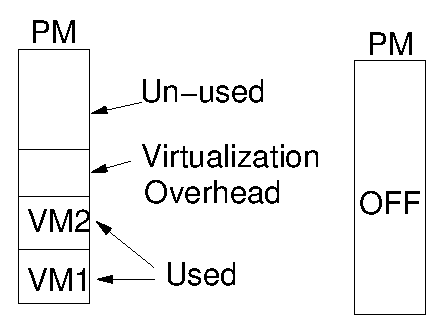
\includegraphics[scale=0.55]{presyn-figures/initially-consolidated.eps} & 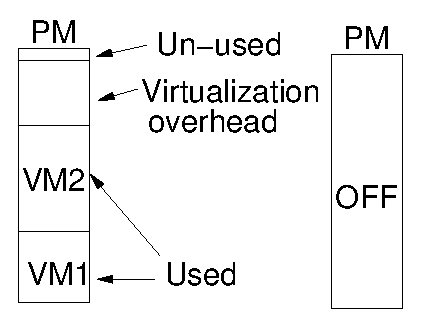
\includegraphics[scale=0.55]{presyn-figures/slight-load-increase.eps} \\
% (a) Initially VMs colocated on a single PM &  (b) Slight increase in load can be accommodated. \\
% 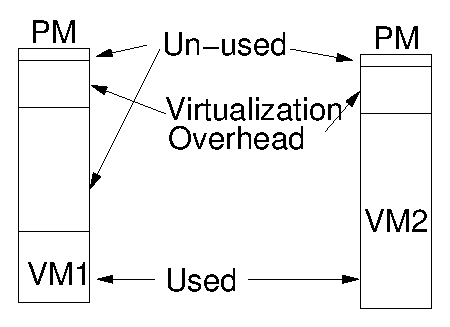
\includegraphics[scale=0.55]{presyn-figures/heavy-load-needs-migration.eps} & 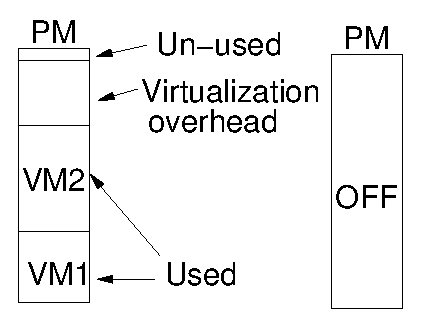
\includegraphics[scale=0.55]{presyn-figures/low-load-migrate-back.eps} \\
% (c) Heavy load requires migration of one VM. & (d) Migrate back when load falls. \\
% \end{tabular}}
% \caption{Server Consolidation and Migration for Dynamic Resource Provisioning.}
% \label{consolidation-migration}
% \end{center}
% \end{figure}

\begin{figure}[t]
\begin{center}
% \noindent\makebox[\textwidth]{% 
\subfloat[VMs colocated on single PM]{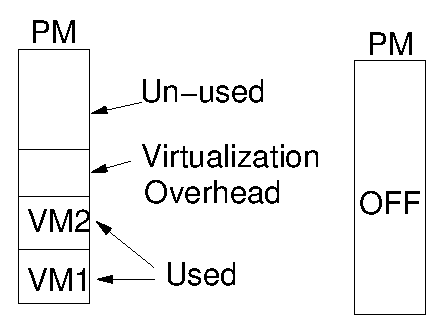
\includegraphics[scale=0.75]{presyn-figures/initially-consolidated.eps}} ~~~~~~~~~~~~~~~~~~~~~~~~
\subfloat[Slight load increase handled]{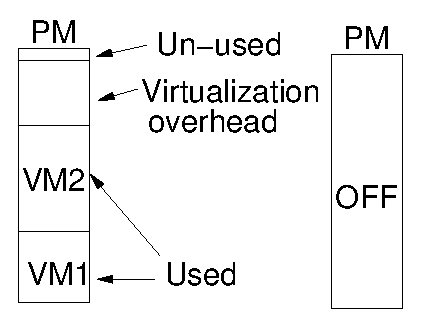
\includegraphics[scale=0.75]{presyn-figures/slight-load-increase.eps}} \\ \vspace{0.15in}
\subfloat[Heavy load requires VM migration]{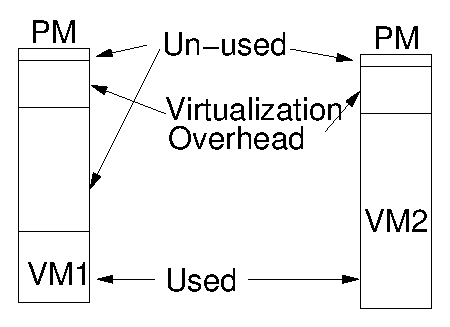
\includegraphics[scale=0.75]{presyn-figures/heavy-load-needs-migration.eps}} ~~~~~~~~~~~~~~~~~~~~~~~~
\subfloat[Migrate back when load falls]{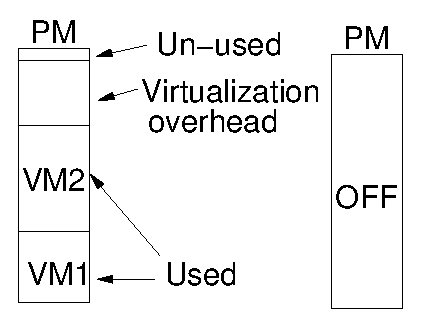
\includegraphics[scale=0.75]{presyn-figures/low-load-migrate-back.eps}}
\vspace{-0.1in}
\caption{Server consolidation and migration for dynamic resource provisioning}
\label{consolidation-migration}
\end{center}
\end{figure}



Most web-based applications are multi-tiered\index{Multi-tiered} and 
virtualization\index{Virtualization}
offers the possibility of hosting each of these tiers (e.g., the 
web-server tier,
the application logic tier and the database server) on separate
elastically provisionable virtual machines. Such differentiated hosting
for various tiers is preferable %to hosting the entire 
%application as a monolithic entity hosted on a single peak-provisioned 
%physical machine since 
as it enables independent resource management and
administration of the different tiers. Additionally, due to
elastic potential of resource allocation to virtual machines,
differentiated hosting on virtual machines can help avoid resource
wastage on under-utilized physical machines.


When applications are instantiated in a virtual
environment, the following major factors affect their 
performance\textemdash{}available network capacity, disk access bandwidth
and virtualization overheads. 
Multiple virtual machines\index{Virtual machine} 
colocated on a single physical machine\index{Physical machine},
compete for resources like CPU, memory, network and disk I/O
and interact in many conflicting ways. 
% Hence, given a set of physical
% machines, a bin-packing problem would need to be formulated to determine
% which subset of virtual machines need to be placed/co-hosted/consolidated
% on each physical machine, to obtain an optimal placement mapping.
In a virtualized environment, the resources available can 
be broadly categorized into two.

\paragraph{I. Resources allocated to the virtual machines.}
Every virtual machine has access to a set of resources, similar
to those available on physical machines.
For example, virtual CPU, VM page cache, virtual disk, etc.
These are
usually statically allocated in today's datacenters~\cite{ec2},
but can be better managed using dynamic provisioning\index{Provisioning}
techniques~\cite{sandpiper, google-live-migration}.

\paragraph{II. Resources in the virtualized host.} These are resources
at the disposal of the virtualized host to support and enable
the functioning of the hosted VMs. For example, apart from 
the virtual CPU allocated to the VMs, the hypervisor\index{Hypervisor} 
and/or Dom0\index{Dom0} 
also need certain CPU allocation to handle the virtualization
overheads~\cite{measuring-cpu-overhead}. 
Similarly, the virtualized host has a 
page cache\index{Page cache} which is used for managing the buffering of 
physical I/O access~\cite{my-cache-or-yours}. 
\\
\\
In this thesis, we address two
important issues related to the management of both
these types of resources more efficiently, towards the overall goal
of optimizing the performance of virtualized applications.

\section{Thesis contributions}
This thesis addresses problems related to improved resource provisioning
and utilization in virtualized environments. In this section, we concretely
state our contributions.

\paragraph{1. Affinity-aware Modeling of CPU usage for Virtualized Applications.}
The first component of this thesis deals with managing the network 
usage of virtual machines and estimating the resulting CPU 
requirement on both the virtual machine\index{Virtual machine} 
and its host physical machine.
Since different tiers of an application require network
communication with each other, placing communicating virtual
machines on the same physical machine\index{Physical machine} 
would reduce physical network 
usage. We define the presence of network traffic between a pair
of VMs as their \textit{network affinity}\index{Network affinity}, 
and state that the
nature of this network traffic is \textit{mutable}\index{mutable} 
(i.e., changing) based on
whether the VMs are colocated\index{Colocated} or 
dispersed\index{Dispersed}. Specifically, the
nature of the network traffic between a pair of VMs
can change between being
intra-PM\index{Intra-PM} and inter-PM\index{Inter-PM} 
depending on whether the VMs are hosted
on the same physical machine or on different physical machines.
We explore the effect of \textit{mutable}
network traffic on CPU usage of colocated and dispersed VMs. More
specifically, the question is, \textit{is the CPU utilization of mutually
communicating VMs dependent on whether the communication happens
intra-PM or inter-PM, and if so, 
how to estimate the target scenario's CPU utilization?}
We make the case that there is significant change in CPU resource
usage of communicating VMs when they are colocated versus when they are 
dispersed, and it is
essential to capture such changes via a model, to assist in
automated server consolidation\index{Server consolidation} 
and VM placement decisions.

We present benchmarking\index{Benchmarking} experiments
which demonstrate impact due to network affinity
on CPU usage of virtual machines and their hosts, when communicating
VMs are colocated as compared to
when they are dispersed. Motivated by these findings, we develop models
that can estimate the ``colocated'' CPU resource usage when VMs transition
from dispersed to colocated placements, and can estimate the ``dispersed''
CPU resource usage when VMs transition from colocated to dispersed
placements. These models predict CPU usage in target 
scenario (colocated/dispersed) based on resource usage profiles 
from source scenario (dispersed/colocated).

Initially, we built models to predict total CPU usage for target scenario,
based on all resource usage profiles like CPU, disk, mutable network
and immutable network usage. However, the maximum error with these 
predictions was found to be around 4 to 6\% absolute CPU usage. 
Consequently, based on our findings that CPU usage is affected only by
\textit{mutable} network traffic levels, we built models to 
predict the difference in (or differential) CPU usage based on only
the mutable network traffic profiles. These models were much more
accurate, with maximum error within 2\%. Finally, we applied these
pair-wise models to multi-VM scenarios using a multi-phase
prediction methodology. This demonstrated that simple models
built on the scale of two VMs could be successfully used to
predict for multi-VM scenarios as well.

\paragraph{2. Using Implicit Caching Hints for {D}isk I/O {R}eduction in Virtualized Environments.}\index{DRIVE}
This component deals with managing the cache resource
usage on a virtualized host machine so as to improve the disk access performance 
of virtual machines.
Due to increased permeation of virtualization-based systems, there is a lot of 
inherent content similarity in systems like email servers, web servers 
and file servers. All this data resides on disk and is fetched by corresponding
applications, as and when required. 
Typically, caches are addressed by block number (hence called 
\textit{location-addressed} caches)\index{Block-cache} and are not
equipped to recognize content similarity across multiple blocks.
Harnessing the content similarity can help 
avoid duplicate disk I/O requests that fetch the same content repeatedly.
In this work, we incorporate intelligent I/O redirection within the 
storage virtualization engine of the device to manage the underlying 
location-addressed cache like a \textit{content-deduplicated} cache.

We build a disk read-access optimization called DRIVE, that
identifies content similarity across multiple blocks in the disk I/O stream, 
and performs hint-based read I/O redirection to improve cache effectiveness,
thus reducing the number of disk reads further.
% than other systems.
A metadata store is maintained based on the VM's disk
accesses and implicit caching hints are collected
for future read I/O redirection\index{I/O redirection}.
The read I/O redirection is performed from within the virtual
block device in the virtualized system, to manipulate the entire
host-cache as a content-deduplicated cache implicitly.
Our trace-based evaluation using a custom simulator\index{Simulator}, 
reveals that
DRIVE always performs equal to or better than the Vanilla system,
achieving up to 20\% better cache-hit ratios and reducing the
number of disk reads by up to 80\%. The results also indicate that
our system is able to achieve up to 97\% content 
deduplication\index{Deduplication} in the host-cache.

\section{Tools and deliverables}
As part of the work in this thesis, we developed several tools and utilities,
that we report here as ``deliverables'' of this thesis. For each of these
tools, their motivation, requirements specification, design and 
implementation are discussed in the Appendix chapters.
\begin{enumerate}
	\item \texttt{LoadGen}: This is a multi-threaded workload generator, 
		that can be used to generate various types of worklaods like
		CPU, disk, network and mixed workloads at pre-specified levels.
		For details, refer to Appendix Chapter~\ref{chap:thesis-loadgen}.
	\item \texttt{SimReplay}: This is a custom cache simulator, with 
		extensions to look into content similarity while operating 
		the cache. For details, refer to Appendix 
		Chapter~\ref{chap:thesis-simreplay}.
	\item \texttt{Preadwritedump}: This is an I/O trace logging and
		collection toolkit, consisting of different tools to perform
		I/O tracing in the Linux kernel and for collecting the logs
		from the kernel datastructures and writing 
		into the persistent filesystem. For details, refer to Appendix 
        Chapter~\ref{chap:thesis-tracing}.
\end{enumerate}

\section{Thesis outline}
The rest of this thesis is organized as follows. 
Chapter~\ref{chap:thesis-litreview} presents brief background 
to cover the scope of this thesis.
In Chapter~\ref{chap:thesis-arescue}, we present our work
related to building network affinity-aware CPU estimation\index{Estimation} models 
for migratory VMs and their host PMs. In Chapter~\ref{chap:thesis-drive},
we present our I/O reduction system called DRIVE\index{DRIVE} which
improves the efficiency of host cache using deduplication-based
I/O redirection. For further evaluation of DRIVE, we 
performed a detailed literature survey comprising over 100+
publications and 350+ datasets. So, in 
Chapter~\ref{chap:thesis-architecting},
we present the findings of our survey, 
which shows that there are no realistic I/O workload datasets 
or benchmarks available that captures content representation.
In Chapter~\ref{chap:thesis-open-directions}, we present
some open directions and future work for this thesis,
and Chapter~\ref{chap:thesis-conclusions} concludes.



\newpage\leavevmode\thispagestyle{empty}\newpage	%for a blank page without page numbering
\chapter{Background \& Literature Review} 
\label{chap:thesis-litreview}

In this chapter, we present a brief background review to cover 
the entire thesis scope. We present the basics of cloud computing, 
usage of virtualization to provide Infrastructure as a Service cloud
computing, as well as the basic mechanisms of network and disk
I/O virtualization. 
% Add the basics of I/O virtualization here, and talk about how the 
% 2 parts of the thesis apply to various aspects of this virtualization
% framework.

\section{Overview of cloud computing and virtualization}
\label{sec:litreviewchap-cloud-virt}
An organization which needs to host multiple services like e-mail servers,
web servers, file downloading servers, e-commerce websites, etc may either opt
to own, maintain and manage their own 
infrastructure (i.e., private\index{Private cloud} 
clouds~\cite{ubuntu-private-cloud}), 
or alternatively, use the services provided by public hosting 
centers (i.e., public\index{Public cloud} clouds~\cite{ec2}). 
In traditional datacenters (before virtualization), multiple
servers would run as separate processes on the same machine and such
mapping would exist from subsets of processes to a set of physical machines.
Guaranteeing resource isolation could be possible only by hosting a single
server on a single physical machine, but would 
cause resource under-utilization
during periods of light loads.

For instance, an auction website may have
periods of heavy load during the day and be comparatively lightly-loaded
during the night. Hence, it may be profitable to the hosting center provider to
host multiple auction websites on the same machine during the night while
assigning them separate machines during the day. However, such adjustments
would need manual intervention or tedious automation to plan/set them up.
Typically, tedious automation and/or manual intervention to provision 
resources based on workload levels, would be well avoided and traditional
hosting centers would just provision the servers for peak load.
However, such static allocation of resources to each server is wasteful
and inefficient because
the server is not expected to be handling peak load at all 
times~\cite{capacity-planning, emerging-research-directions}. Also, with
such static allocation, initial deployment of a server in the data-center
will involve procurement and setup delays of the physical 
machines\index{Physical machine}~\cite{xen-art-of-virtualization}. 

Virtualization\index{Virtualization} helps to avoid
such pitfalls, by enabling dynamic resource allocation and 
quicker deployment
of services. Instead of installing new hardware for deploying/scaling a server
in the data-center, virtualization 
allows transparent, on-demand deployment on a few
processors in an existing multi-processor machine and avoids new machine
procurement delays~\cite{xen-art-of-virtualization}. 
Virtualization allows accommodation of varying load-levels by
on-demand resource allocation~\cite{xen-art-of-virtualization-revisited}
and also helps reduce application downtime~\cite{google-live-migration}. 
Due to above benefits of virtualization, 
many hosting centers have moved to providing 
Infrastructure as a Service (IaaS)\nomenclature{IaaS:}{Infrastructure as a 
Service}\index{IaaS}~\cite{ec2, azure} instead of
Hardware as a Service (HaaS)\nomenclature{HaaS:}{Hardware as a Service}\index{HaaS}.
The primary difference between HaaS and IaaS is that the 
former involves use or leasing of physical
hardware/machines whereas the latter involves 
leasing of virtual resources/machines\index{Virtual machine}.


\subsection{Virtualization}
Virtualization is a technology that allows abstraction of network, storage
and compute services, by providing a software middle-layer between the
physical hardware and the applications that run on it.
Hence, each physical machine (PM)\index{PM} 
can host multiple virtual machines (VMs)\index{VM},
such that each virtual machine sees an
abstraction of resources on which it executes. This makes it easy
to start, stop, move or increase the number of virtual machines hosted
on one or more physical machines.

To motivate the use of virtualization, let us consider a similar example.
Suppose an organization needs to host fifty software 
applications\textemdash{}webservers, email servers, file servers and so on.
Based on some back-of-the-envelope calculation of resource requirements,
suppose twenty physical machines are procured for this purpose.
In the absence of virtualization, a subset of servers each, would be hosted
on each physical machine and each might be typically
peak-provisioned~\cite{berkeley-view}. 
The selection of which subset of servers can/should
be hosted together on a single machine may be random or may depend on
considerations like
OS platform issues, licensing issues, hardware capacity, software/hardware
version compatibilities, etc. Some subset of servers may even be grouped
together if they have mutually exclusive resource requirements (say
CPU-bound webservers and 
IO-bound database servers 
hosted together~\cite{dynamic-provisioning-multi-tier}) 
because there is a perceived high-level guarantee that neither 
one will encroach on the resource
requirements of the other, 
thus providing approximate resource isolation.
However, guarantees of resource isolation can be provided only with kernel 
changes and/or real-time operating systems~\cite{enforcing-isolation}.

A user who invests in hosting services would prefer to get hard guarantees
on resource and performance isolation instead of being subject
to the vagaries of resource utilization of other colocated processes
or applications. 
Moreover, in case of \textit{public clouds}, 
the user would also prefer to be paying only for
utilized resources and not for unused resources~\cite{berkeley-view}. This is
where virtualization offers a good solution. A virtual machine gives
an entire machine-like resource environment with usability of any
operating system. And thus, the user need only be charged for the resources
being allocated to their virtual machine~\cite{ec2}.

Virtualization allows each server process to be provided with its own
resource environment and guarantees a fixed amount of resources such that
its resource availability and performance levels will not be affected by
any other colocated process's resource usage.
Such guarantees are possible owing to the
virtualization middle-layer, or the 
Virtual Machine Monitor (VMM)\index{VMM}, which
arbitrates communication back-and-forth between the applications and the
hardware. Basically, each application gets
its own (virtualized) environment, 
known as a \textit{Virtual Container} or a
\textit{Virtual Machine} and it may be even unaware that 
its container is not a
physical machine with access to real hardware i.e. virtualization is
transparent to the applications/services themselves. Each virtual machine
runs like a separate operating-system instance and has interfaces for
direct or indirect access to the physical hardware. The OS\footnote{OS stands
for Operating System} executing within the virtual machine is referred to
as a \textit{guest OS}\index{Guest OS} while the original 
operating system on the physical
machine which provides the virtualization support is referred to as
the \textit{host OS}\index{Host OS}.

Example instantiations of
virtualization-based solutions are, (i) users/clients hosting their
applications on a remote datacenter\index{Datacenter} 
and negotiating for service level agreements\index{SLA}
%(henceforth referred to as a \textit{Public Cloud}).
and (ii) enterprises hosting applications and services on a
private self-managed cluster of machines, for internal and external
access.
%(henceforth referred to as a \textit{Private Cloud}).
In the latter
example, both the user and the provider may be one and the same.
Virtualization offers benefits to both users and providers 
of the datacenter.
Traditionally, an end user would be burdened with planning, acquiring
and deployment of infrastructure, 
and also regular maintenance~\cite{berkeley-view}. The end-user
would require to plan software updates and hardware upgrades as the system
grows, and also manage low-level decisions to maintain performance
requirements. However, with virtualization, the end user is responsible only
to pay for the resources on-demand, while receiving guarantees on performance.
The end-user can be agnostic of physical hardware issues. At the back-end,
the service provider benefits by way of potential opportunities to
effectively multiplex available resources~\cite{vm-multiplexing}, 
provide on-demand \& scalable service~\cite{google-live-migration} 
that is centrally managed, and cut down on expenses.

\begin{figure}[t]
\begin{center}
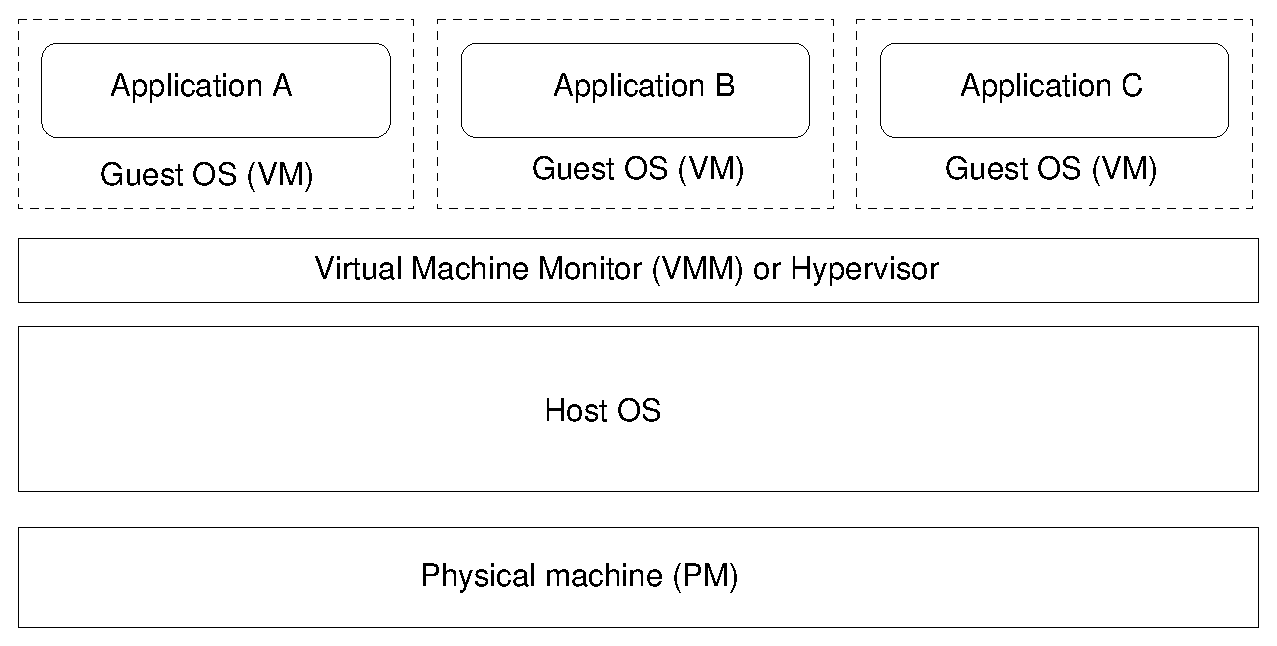
\includegraphics[height=7cm, width=14cm]{first-aps-figures/virtualization-arch.eps}
\caption{Virtualization framework architecture: \textit{A physical machine is 
virtualized using a VMM such that it is capable of hosting multiple virtual 
machines that have their own operating systems (OS) each. The VMM is thus, a
middleware that handles and delegates the responsibilities related to virtualization
of the physical machine.}} 
\label{virtualization-arch}
\end{center}
\end{figure}

\subsection{Virtualization techniques}
\label{virtualization-tech}
There are various virtualization techniques: \textit{full-virtualization}~\cite{vmware-paravirtualization},
\textit{para-virtualization}~\cite{xen}, \textit{OS-level
virtualization}~\cite{quantifying-the-performance-isolation-properties}
and \textit{hardware-assisted virtualization}~\cite{kvm}.
Fig.~\ref{virtualization-arch} shows the basic architecture of the
virtualization framework. As seen in the figure, a host operating
system, instrumented with the 
Virtual Machine Monitor (VMM)\index{VMM} or Hypervisor\index{Hypervisor},
executes on the physical machine, 
and one or more VMs, containing guest operating systems, execute on top 
of the virtualization layer.


\underline{Full-virtualization}\index{Full-virtualization}: In 
this technique, the guest 
OS can run unmodified within the virtual machine. This is made 
possible by the use of Binary translation and
Direct execution techniques~\cite{vmware-paravirtualization}. 
\textit{Binary translation} refers to ``on-the-fly substitution'' 
of traditional guest OS instructions with a virtual sequence of 
instructions and, \textit{Direct execution}
strategy is adopted for executing user-level code. So the
guest OS is completely decoupled from the underlying hardware by the
virtualization layer.
Binary translation is used in VMware's full-virtualization 
solution~\cite{vmware-paravirtualization} due to challenges
in virtualizing privileged operations, like I/O instructions. This is
because if a guest OS is directly allowed to execute the privileged I/O
instructions, it could alter the
state of other guest OSes and compromise security. 

\underline{Para-virtualization}\index{Para-virtualization} tries 
to address the concern of
I/O virtualization another way, by making changes to the guest
OS such that privileged I/O instructions cause traps to the hypervisor and are
executed by it on behalf of the guest OS. For example, request for an I/O
operation by the guest OS will
be made in the form of a function call that does not actually perform
the I/O operation, but merely requests the hypervisor to perform it.
The hypervisor will execute the I/O after checking for requisite permissions,
and will intimate the guest OS when task is over.

\underline{OS-assisted virtualization}\index{OS-assisted virtualization}: 
In this technique, guest operating systems\index{Guest OS} are processes 
that are allocated different namespaces such that
they seem to be separate machines altogether. However, in OS-level
virtualization, the same host OS\index{Host OS} kernel also supports 
the guest processes.
The advantage of full-virtualization and paravirtualization over OS-level
virtualization is that they can support heterogeneous operating system
distributions as guest OSes, like Linux, BSD and Windows
XP~\cite{xen-art-of-virtualization}. 
Although paravirtualization is also an OS-assisted form of virtualization 
requiring all privileged instructions to be executed by the virtualization
layer, the difference is that para-virtualization can support
different guest operating systems whereas OS-level virtualization cannot.

\underline{Hardware-assisted virtualization}\index{Hardware-assisted virtualization}: 
In this technique,
the hardware is enhanced with virtualization awareness such that
the CPU itself traps the privileged/sensitive instructions and emulates
the instructions in hardware instead of software, hence obviating the need
for binary translation or paravirtualization. Hardware-assisted virtualization
is also a form of full virtualization since the guest OS can remain ignorant
of the virtualization involved~\cite{hardware-assisted-wiki}.
% However, hardware assisted virtualization technique
% is still in its infancy and has not become much popular yet.

Based on the above
types, there are several virtualization technologies
like Xen~\cite{xen-art-of-virtualization}\index{Xen},
Vmware~\cite{vmware-paravirtualization}\index{Vmware},
KVM~\cite{kvm}\index{KVM} and OpenVZ~\cite{OpenVZ}\index{OpenVZ}. 
Xen is an
example of para-virtualization, KVM and VMware are examples of
full-virtualization and OpenVZ is an example of OS-level
virtualization.


\section{Basics of I/O virtualization}
\label{sec:litreviewchap-io-virtualization}
%Need another paragraph to begin the description of these basics.
All regular instructions involving CPU computation within the
virtual machines are executed similarly to the physical machine
case, since no
switch between kernel and user modes is required during execution of
CPU instructions. However, in case of I/O operations, not only are
context switches between kernel and user modes required,
but also permissions and security are of paramount importance.
Basically, I/O operations have a higher access level
than CPU operations, and hence it is necessary for the Hypervisor
to intercept and arbitrate the I/O operations requested 
by the virtual machines. In this section, we present 
a brief background on I/O virtualization techniques, towards
setting up the background for work done in this thesis.

\subsection{Network I/O virtualization}


\begin{figure}[t]
\centering
% 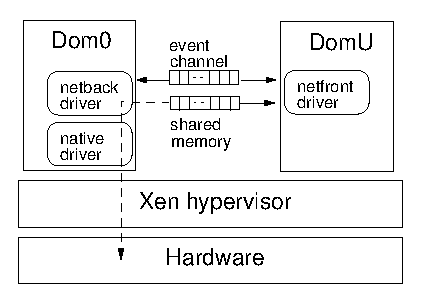
\includegraphics[height=1.75in]{jss-figures/xenarch.eps}
\hspace{-0.2in} \subfloat[Xen's driver domain model]{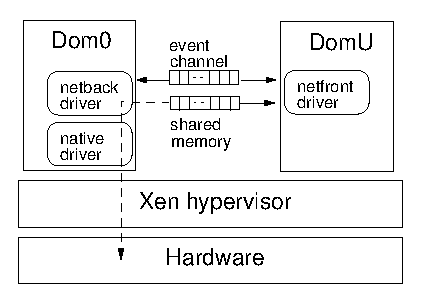
\includegraphics[scale=1]{jss-figures/xenarch.eps}} ~~~~~~~~~~~~~~~~~~~~
\subfloat[KVM's direct I/O model]{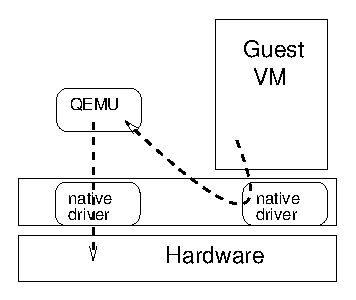
\includegraphics[scale=1]{jss-figures/kvmarch.eps}}
\caption{Different I/O virtualization architectures\textemdash{}Xen and KVM}
\label{fig:xen-vs-kvm}
\end{figure}

Xen~\cite{xen-art-of-virtualization} is a 
para-virtualization\index{Para-virtualization} 
based technology while KVM~\cite{kvm} is 
full-virtualization based\index{Full-virtualization}.
\nomenclature{KVM:}{Kernel Virtual Machine}\index{KVM}
Fig.~\ref{fig:xen-vs-kvm}(a) shows the Xen\index{Xen} 
virtualization architecture depicting 
Dom0\nomenclature{Dom0:}{Domain zero in Xen (driver domain)}\index{Dom0}\textemdash{}which 
is the privileged management/driver domain, and 
DomUs\nomenclature{DomU:}{User Domain in Xen (guest domain)}\index{DomU}\textemdash{}which 
are the guest virtual machines. 
All network I/O operations
of the guest VMs are arbitrated by Dom0 via a shared memory interface
termed Tx and Rx I/O rings. 
An event channel notification mechanism is used to notify events
to the domains, for example, notification to DomU regarding a 
received packet or notification to Dom0 for a packet to be
transmitted from DomU.
The \texttt{netfront}\index{Netfront} 
and \texttt{netback}\index{Netback} 
drivers, in DomU and Dom0 respectively,
coordinate the data exchange between the domains,
and the native driver in Dom0 coordinates exchange with
the physical network interface. 
%The above procedure is followed
%for both network operations as well as network-assisted disk I/O operations.

The I/O architecture used by Xen\index{Xen} with para-virtualization 
is referred to as the Driver domain I/O model. 
On the other hand, KVM\index{KVM}\cite{kvm-whitepaper} 
is an example of hardware-assisted virtualization (also full-virtualization),
and uses another model for I/O, wherein virtual machines are run as 
processes on the host and I/O
processing is done by the QEMU~\cite{qemu}\index{QEMU} emulator in userspace.
In this architecture, there is no separate driver domain to handle 
privileged instructions, hence it is called 
the Direct I/O model~\cite{net-fairness-visa-2010}.
% performs dynamic binary translation of all guest
%instructions and executes them directly on the physical host hardware.
%This is called the Direct I/O model~\cite{net-fairness-visa-2010} and has no 
%separate
%driver domain to handle privileged instructions. 

Due to arbitration of DomU's I/O access by Dom0,
network activity of guest VMs results in additional
CPU utilization at Dom0. However, since dispersed VMs communicate
by accessing the physical network interface as opposed to colocated VMs
that communicate ``locally'', network communication between
colocated and dispersed VMs results in different CPU overheads.
In the first component of our thesis, we study the Dom0 CPU overheads
with colocation and dispersion of virtual machines and
build resource estimation models based on these findings.
\\
\\
In the above description, both Xen and KVM technologies are shown to 
have different I/O architectures, and the first component of our 
thesis deals with both architectures to demonstrate the difference
in CPU overheads for communicating VMs.
However, subsequently in 2008, 
an I/O processing framework known as \texttt{virtio}\index{Virtio} was 
proposed in~\cite{virtio}, which is a generic, modular and pluggable 
platform that can be used transparently with 
any hypervisor. The motivation of this framework was to
make hypervisor development
independent from the development of virtualization-based 
I/O drivers~\cite{virtio}.
This new framework shaped the design of our disk I/O redirection system
in the second component of this thesis, as explained next.

\subsection{Disk I/O virtualization}
A virtual machine's storage is called a virtual disk, can be either
an image file or a block device~\cite{ip-networked-storage}, and can be 
located on either a local disk attached to the 
physical machine, or network-attached as well.
When the virtual disk is located on a locally attached disk on the 
physical machine, it is referred to as Direct-attached 
storage (DAS)\nomenclature{DAS:}{Direct-attached Storage}\index{DAS},
whereas Network-attached storage (NAS)\index{NAS} and Storage Area Networks (SAN)\index{SAN}
are examples of storage that are accessible over the network.
Moreover, the difference between the virtual disk being a file or a
block device is that in case of a file, the virtual machine's ``disk-access
requests'' are translated into file-access requests by the Hypervisor, 
and then once again converted into block layer requests at the host
physical machine. This double-indirection is avoided in the case
where the virtual disk is itself a block device, and accessible using
block layer semantics, for 
eg. iSCSI\nomenclature{iSCSI:}{Internet Small Computer Systems Interface}\index{iSCSI}
SAN device~\cite{iscsi} or 
LVM-configured\nomenclature{LVM:}{Logical Volume Manager}\index{LVM}
storage volumes~\cite{lvm} on the physical machine.


%This section covers
%background related to disk I/O virtualization, and implications
%on host cache management.


\begin{figure}[t]
   \centering
   \subfloat[KVM]{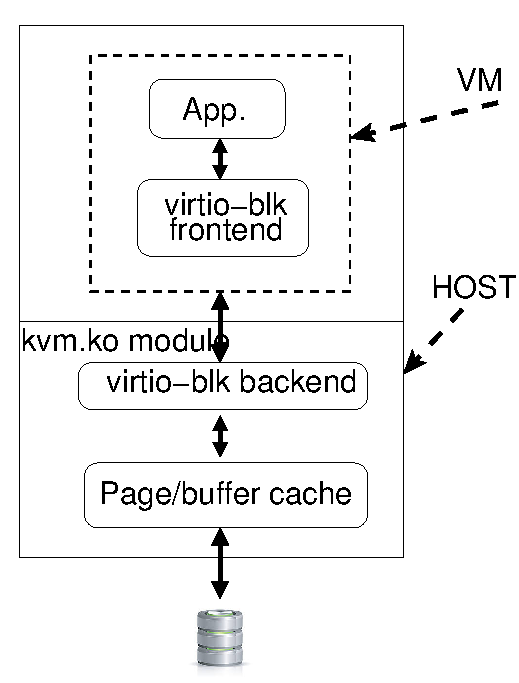
\includegraphics[scale=0.6]{confided-figures/main/kvm-disk-io.pdf}} ~~~~~~~~~~~~~~~
   \subfloat[Xen]{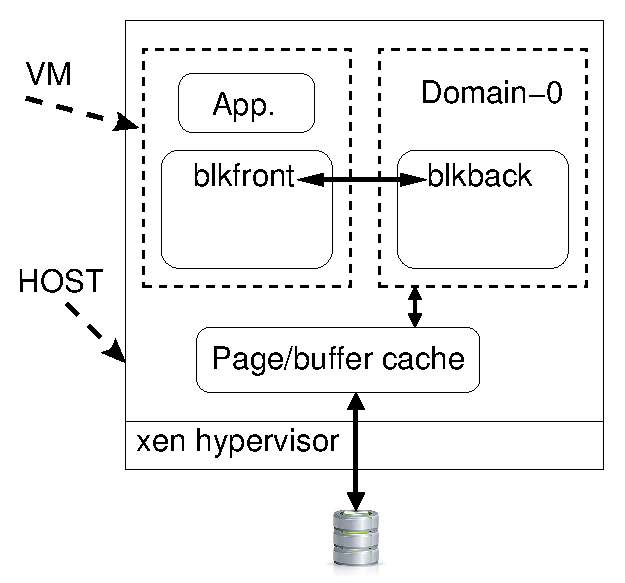
\includegraphics[scale=0.6]{confided-figures/main/xen-disk-io.pdf}} 
   \caption{Split-driver architecture for virtual block devices in KVM and Xen virtualization.}
   \label{fig:disk-io-arch}
%    \vspace{-0.2in}
\end{figure}

Irrespective of the type of storage used, the access to virtual disk is
performed via virtual block drivers within the VM. 
% In this sub-section, we 
% present background related to the paravirtualized virtual disk drivers,
% also referred as virtual block drivers.
As mentioned above, a new and emerging framework for 
virtual I/O device drivers is \texttt{virtio}~\cite{virtio}\index{virtio}. 
The basic concept of \texttt{virtio} is a split-driver
architecture, i.e., a pair of \texttt{frontend} 
and \texttt{backend} drivers that communicate with each other using
a ring-buffer mechanism.
The virtual machine hosts the \texttt{frontend} driver and forwards the
request to the corresponding \texttt{backend} driver hosted in the 
hypervisor or VMM\index{VMM}.
Virtio is developed in Hypervisor-agnostic fashion, with the only
constraint that Hypervisor and the guest OS are able to interact
with virtio using appropriate ring-buffer handling mechanisms.
Hence, virtio can be used
with a variety of Hypervisors like Xen, KVM and lguest virtualization 
solutions~\cite{virtio}.

The de-coupling of the virtual block device driver 
into \texttt{frontend}\index{Frontend} and \texttt{backend}\index{Backend} drivers
makes \texttt{virtio}
a generic virtual I/O mechanism, which can work on multiple hypervisors
and platforms. Currently, \texttt{virtio} is used as a high-performance
I/O mechanism in KVM~\cite{kvm}\index{KVM} virtualization technology. 
The paravirtualized block driver in Xen~\cite{xen} architecture also follows
the split-driver paradigm, wherein a privileged VM (Domain-0) hosts the 
\texttt{backend} driver. The split-driver architecture for virtual block devices
in Xen and KVM is illustrated in Fig.~\ref{fig:disk-io-arch}.
The communication between the \texttt{frontend} and \texttt{backend} block drivers is 
accomplished via a ring buffer transport mechanism, wherein each read
request is described in a descriptor placed into the ring buffers. Each
read request descriptor includes the block ID/address (to be read) and a 
buffer (into which the data is to be copied). 
In the second component of our thesis, we present a hint-based read
I/O redirection method positioned within the \texttt{frontend}
driver in a virtual machine, which can manipulate the downstream 
host cache in a content-deduplicated
fashion to improve its caching efficiency.

\\
\\
In this chapter, we presented a brief background review of the area of
cloud computing via virtualization, toward the scope of this thesis.
Specifically, the discussion of network 
I/O virtualization\index{I/O virtualization} is relevant
to the first component of this thesis 
while the discussion on disk I/O virtualization corresponds to 
the second component.
%addressed in Chapters~\ref{chap:thesis-drive} and \ref{chap:thesis-architecting}).
In the rest of this thesis, we present more detailed literature review 
and background details within each chapter as well, as appropriate.

%moved the following into introduction chapter.
%\\
%\\
%The rest of this thesis is organized as follows. In 
%Chapter~\ref{chap:thesis-arescue}, we present work
%related to building affinity-aware CPU estimation\index{Estimation} models 
%for migrating VMs and their hosts. In Chapter~\ref{chap:thesis-drive},
%we present our I/O reduction system called DRIVE\index{DRIVE} which
%improves the efficiency of host cache using deduplication-based
%I/O redirection. For further evaluation of DRIVE, we 
%performed a detailed literature survey comprising over 100+
%publications and 350+ datasets. So, in 
%Chapter~\ref{chap:thesis-architecting},
%we present the findings of our survey, 
%which shows that there are no realistic I/O workload datasets 
%or benchmarks available that captures content representation.
%In Chapter~\ref{chap:thesis-open-directions}, we present
%some open directions and future work for this thesis,
%and Chapter~\ref{chap:thesis-conclusions} concludes.


\newpage\leavevmode\thispagestyle{empty}\newpage	%for a blank page without page numbering
\chapter{Affinity-aware Modeling of CPU usage for Virtualized Applications}
\label{chap:thesis-arescue}

\section{Introduction}
\label{sec:arescue-intro}

In traditional datacenters, the practice is to either follow
a dedicated model and provision servers for peak loads, or share
resources in a best-effort manner that offers no
guarantees~\cite{resource-overbooking}.
For example, an auction website may be hosted on a single PM
in order to guarantee that it has enough resources to face peak loads.
However, this
results in under-utilization of resources and wastage of power during
low loads, say, when the auction website is idle during night.
Alternatively, co-hosting the auction website with another service 
in simply a
best-effort manner will be insufficient when either of the
co-hosted services is bombarded with heavy load.
Resource utilization can be maximized while still ensuring performance
guarantees through dynamic resource provisioning~\cite{sandpiper, 
vm-multiplexing}, by adopting virtualization
and consolidating/co-hosting multiple services (like
auction websites and email servers) as VMs on the same physical
machine~\cite{entropy}.

Several to-be-virtualized applications have data dependencies
between each other or among their components.
Example instantiations are, (i)~a multi-tier web-based application has
exchange of data
between its components\textemdash{}web-server, application logic server
and the database, and 
(ii)~heavily parallelized applications~\cite{high-consuming-parallel}
which have distributed computing tasks with mutual data dependencies.
\textit{Server consolidation} refers to mapping a set of applications/servers
to instances hosted within
virtual machines, in such a way as to maximize the utility of the
available infrastructure~\cite{load-balancing}.
Thus, server consolidation can facilitate sharing of available resources
among the tiers of a single application or 
across tiers of multiple applications,
using dynamic resource allocation and virtual machine
migration techniques~\cite{sandpiper, adaptation-engine}.


\begin{figure}[h]
	\centering
	\subfloat[Before Consolidation]{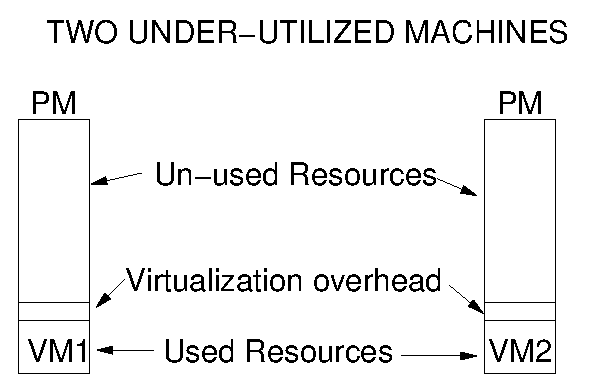
\includegraphics[height=4cm,width=5cm]{figures/before_consolidation.eps}}
	~~~~~~~~~~~~~~~~~~~~~~~~
	\subfloat[After Consolidation]{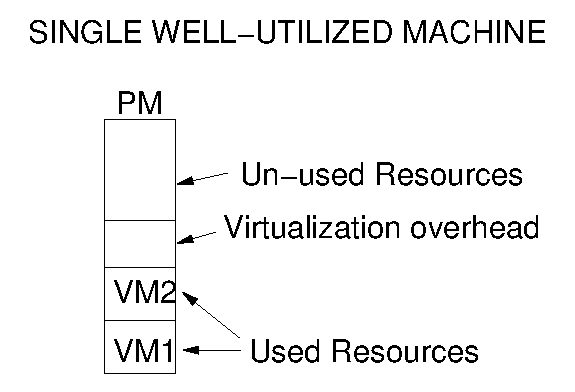
\includegraphics[height=4cm,width=5cm]{figures/after_consolidation.eps}}
\caption{Server Consolidation, via Virtualization, for efficient resource multiplexing.}
\label{virtualization-enables-consolidation}
\end{figure}

An example consolidation scenario is shown in Fig.~\ref{virtualization-enables-consolidation}, 
where two virtualized server instances are moved to or co-hosted on a single physical machine 
such that only one physical machine is sufficient to host both services and
the other machine which becomes idle can be powered off.
In the ``Before Consolidation'' case of Fig.~\ref{virtualization-enables-consolidation}(a), 
each physical machine is executing a single lightly-loaded virtual machine each. 
Here, power is being wasted in keeping both physical
machines ON though under-utilized. In the ``After Consolidation'' case,
both VMs have been moved to one of the physical machines. 
If both the VMs and the corresponding virtualization overheads can be accommodated
on a single PM,
the other resultant unused PM can be switched OFF. Such consolidation and
powering off of unnecessary resources results in better resource
utilization and saves copious amounts of power
(otherwise used for supplying power to machines as well as for cooling) in
the data-center.

\underline{Colocated and dispersed VMs:} When applications are 
instantiated in a virtual
environment, two major factors affect their performance\textemdash{}available
network capacity and virtualization-related CPU overhead,
and these factors vary based on whether the communicating VMs
are located on the same host or on different hosts~\cite{virtual-putty}.
\emph{Colocated}\index{Colocated} 
virtual machines (VMs\nomenclature{VM:}{Virtual machine}\index{VM} 
hosted on the same PM\nomenclature{PM:}{Physical machine}\index{PM}) incur 
different virtualization overheads for mutual network
communication as opposed to \emph{dispersed}\index{Dispersed} VMs 
(VMs placed on different PMs).
It is claimed in \cite{virtual-putty} that transitioning
between colocated and dispersed placements for communicating VMs
can result in a change in their CPU requirements. However, empirical
quantification is lacking.

\underline{Network affinity:} In general, VMs are said to have
\textit{network-affinity}
%\nomenclature{Network-affinity:}{Two VMs have 
%\textit{network-affinity} if they have network communication with each other.}
for each other if they have 
network communication between them~\cite{virtual-putty, starling}.
When VMs are colocated, the network traffic between them
is defined as being \textit{intra-PM}, whereas when they are dispersed,
it is \textit{inter-PM} network traffic.
Since migration of a VM can potentially change the nature of network
traffic between being \textit{intra-PM} and \textit{inter-PM}, depending 
on the source and destination hosts for migration, we define this
as the \textit{mutable} nature of network affinity, as explained next.

\underline{Mutable nature of network affinity:} Given a set of VMs, some 
of which may have network communication with one another, every 
``communicating pair'' of VMs is said to have network affinity for each other.
A migration of any one VM can, but need not necessarily, cause the nature of
network traffic between a VM pair to change from being \textit{intra-PM}
to \textit{inter-PM}, or from being \textit{inter-PM} to \textit{intra-PM}.
For example, suppose there are 4 VMs hosted on 4 PMs, as illustrated
in Fig.~\ref{fig:mutable}(a). The VM pairs that have
network affinity are, (i)VM1 $\leftrightarrow$ VM2,
(ii)VM2 $\leftrightarrow$ VM3 and,
(iii)VM3 $\leftrightarrow$ VM4. 

\begin{figure}[h]
\begin{center}
	\subfloat[Initial configuration]{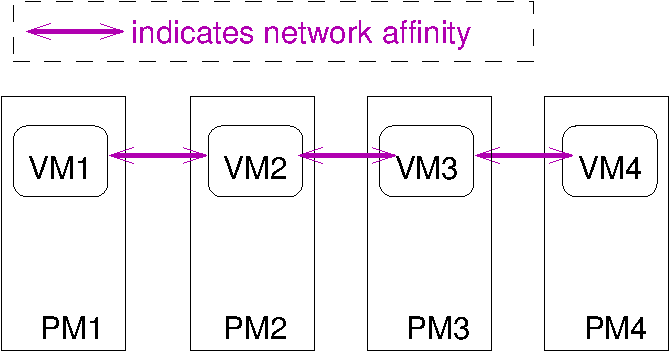
\includegraphics[scale=0.6]{arescue-figures/mutable-immutable.pdf}}
	~~~~~~~~~~~~~~~~~~~~~~~~~~
	\subfloat[VM3 migrates to PM2]{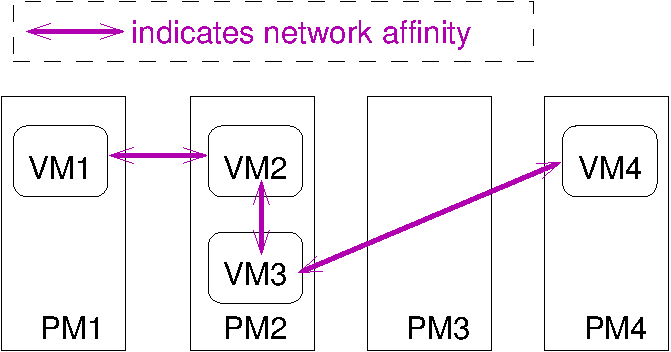
\includegraphics[scale=0.6]{arescue-figures/mutable-immutable-2.pdf}}
	\caption{Example to demonstrate \textit{mutable} and \textit{immutable} network affinity.}
\label{fig:mutable}
\end{center}
\end{figure}

In the initial state (refer Fig.~\ref{fig:mutable}(a)), all VMs are
hosted on different PMs (i.e. dispersed), hence the network traffic
in each case is \textit{inter-PM}. Suppose VM3 is now migrated from
PM3 to PM2, it gets colocated with VM2, resulting in the 
configuration shown in Fig.~\ref{fig:mutable}(b). 
After the migration, the nature of traffic between VM2 and VM3
has changed from \textit{inter-PM} to \textit{intra-PM}, whereas VM2
continues to have \textit{inter-PM} network affinity with VM1.
Thus, migration of VM2 caused its network traffic with VM3 to 
change nature, while its traffic with VM1 remained unchanged. We differentiate
these two types of network traffic as \textit{mutable} and \textit{immutable}
network traffic.
Basically, for a given VM migration, \textit{mutable} network traffic 
is that which changes nature between \textit{inter-PM} and \textit{intra-PM},
and \textit{immutable} network traffic is that whose nature does not change
due to migration.

We present benchmarking experiments
which demonstrate impact due to network affinity
on CPU usage of virtual machines and their hosts, when communicating
VMs are colocated as compared to when they are dispersed. 
Motivated by the benchmark findings, we develop models
that can estimate the ``colocated'' CPU resource usage when VMs transition
from dispersed placements to colocated, and can estimate the ``dispersed''
CPU resource usage when VMs transition from colocated placements to dispersed. 
These models predict CPU usage in target
scenario (colocated/dispersed) based on resource usage profiles
from source scenario (dispersed/colocated).

Initially we built models to predict total CPU usage for target scenario,
based on all resource usage profiles like CPU, disk, mutable network
and immutable network usage. However, the maximum error with these
predictions was found to be around 4 to 6\% absolute CPU usage.
Consequently, based on our findings that CPU usage is affected only by
\textit{mutable} network traffic levels, we built models to
predict the difference in CPU usage based on only
the mutable network traffic profiles. These models were much more
accurate, with maximum error within 2\%. Finally, we applied these
pair-wise models to multi-VM scenarios using a multi-phase
prediction methodology. This demonstrated that simple models
built on the scale of two VMs could be successfully used to
predict for multi-VM scenarios as well.
%In our work, we perform empirical quantification of 
%the CPU resource that Xen-based VMs would require if they were
%to be migrated for colocation or dispersion (splitting up of 
%previously-colocated VMs). 
%
%We are concerned with CPU utilization required to handle network
%In Xen virtualization environment, a
%privileged virtual machine (called Domain-0 or 
%Dom0\index{Dom0}\nomenclature{Dom0:}{Privileged domain or privileged virtual 
%machine or Domain-0}) manages network 
%traffic for the guests (called User Domain or 
%DomU\index{DomU}\nomenclature{DomU:}{User domain or Domain-U})
%and utilizes CPU proportional to network traffic volume.
%In this work, we explore the effect of
%network-affinity on CPU usage of colocated and dispersed VMs. More
%specifically, \textit{what is the effect on CPU utilization of mutually
%communicating VMs based on whether they are colocated or dispersed?}
%An important consideration for migration and consolidation related
%decisions is the expected resources required for the VM
%on the target machine. The consolidation of
%VMs into a colocated set and the migration of VMs to dispersed
%placements, can result in different CPU resource requirements.
%The focus of the first component of this thesis, is to build
%\emph{affinity-aware} models that can predict expected CPU
%resource requirements\textemdash{}upon colocation or dispersion of VMs.
Our contributions are,
\begin{enumerate}	
\item \emph{Event profiling} of intra-PM and inter-PM network
	communication paths in Xen, using \texttt{Xenoprof}~\cite{xenoprof}.
\item \emph{Benchmark} CPU resource requirements
of VMs with different levels of network-affinity
in colocated and dispersed configurations.
\item Perform the above benchmarking step for both Xen and KVM virtualization environments,
	showing that a linear relationship between network usage and the resulting CPU overhead
	exists in both.
\item Develop \emph{pair-wise affinity-aware} models to predict \textit{total}
	as well as \textit{differential} CPU usage, when a pair of VMs move between
	dispersed and colocated placements.
\item Apply above pair-wise models to \emph{multi-VM scenarios}, where
	a single migrating VM has more than one neighboring
	VMs with which it exhibits network-affinity, both on source \& target PMs.
\item Present a \emph{comprehensive evaluation} using synthetic 
	workloads \& benchmark applications,
	of the models as well as application to multi-VM scenarios.
\end{enumerate}

\noindent The rest of this chapter is structured as follows. 
Section~\ref{sec:arescue-background}
presents background regarding network virtualization in Xen and KVM, and
problem statement is presented in Section~\ref{sec:arescue-problem}.
Section~\ref{sec:arescue-benchmark}
presents empirical benchmarking of the effects of relative placement on
CPU usage of communicating VMs, in both Xen and KVM virtualization environments.
Section~\ref{sec:arescue-our-approach} presents our approach to
build affinity-aware models to predict CPU usage for Xen DomU and Dom0
and Section~\ref{sec:arescue-experimental-eval} presents evaluation 
of the models.
Section~\ref{sec:arescue-related-work} presents related work in juxtaposition
with our work and 
in Section~\ref{sec:arescue-open-directions}, we
present our ideas for future work.
%in the area of affinity-aware CPU usage modeling and 
Section~\ref{sec:arescue-conclusions} concludes the chapter.



\section{Background}
\label{sec:arescue-background} This section recalls the concept of network I/O
virtualization in Xen\index{Xen} and KVM\index{KVM} 
(previously presented in detail in
Section~\ref{sec:litreviewchap-io-virtualization}), and supplements it
with an event profiling study of network virtualization in Xen.

\subsection{Recalling the basics of network I/O virtualization}
As discussed in Chapter~\ref{chap:thesis-litreview}, network I/O 
virtualization technologies are:
\begin{enumerate}
\item Para-virtualization based driver domain I/O model,
\item Emulation-based direct I/O model and
\item Virtio-based split-driver I/O model
\end{enumerate}
Note that, both the driver domain I/O model and the virtio model 
have the concept of a split-driver, with the difference
that virtio can be used even in para-virtualization setups, eg Xen.
A split-driver architecture consists of
\texttt{frontend} and \texttt{backend} drivers, of which the 
\texttt{backend} driver is responsible to communicate with 
native network drivers and get the I/O performed on behalf of 
virtual machines. 

An in-depth survey of various shared-memory optimizations
for inter-virtual-machine (i.e. intra-PM) communication
is presented in \cite{shared-mem-optimizations}---and it
presents optimizations in both the para-virtualization
and emulation-based-virtualization setups.
In all above cases, for network communication between VMs 
colocated on a single PM, the native driver 
does not need to be invoked at all whereas
if VMs are hosted on different PMs, physical network
communication is essential. 
This difference manifests as different
CPU overheads for the VMs and the physical hosts 
concerned. In this section, 
we present an event profiling study of CPU overheads in both scenarios,
in the Xen paravirtualization setup.

\subsection{Profiling study of network I/O virtualization}
% Xen uses an inter-domain shared memory mechanism to share data between
% colocated VMs. 
To further motivate the study of differences in communication between
colocated and dispersed virtual machines, we performed a detailed 
profiling-based study of Xen's\index{Xen} 
networking architecture and 
implementation~\cite{xen-internals, xen-networking, linux-networking}. 
% The major difference between dispersed
% and colocated communication is that 

A common optimization in the network communication in colocated case is that 
packet check-summing
(both calculation and verification) is not performed since it is assumed 
that memory copying (performed in colocated case) is quite reliable as 
opposed to physical network transmission (corresponding to dispersed case). 
Additionally, when Xen-based VMs are colocated, they are
connected via a layer 2 software bridge and hence a packet 
transmitted from one VM to another colocated VM is locally delivered 
on the bridge itself. On the other hand, when communicating VMs 
are on different PMs, a packet transmission by one VM
is forwarded over the software bridge, 
DMA-copied\nomenclature{DMA:}{Direct Memory Access}\index{DMA}
into the network interface 
card's (NIC\nomenclature{NIC:}{Network Interface Card}\index{NIC}) 
buffer, and placed on the network link by the NIC. This
transmitted packet is then received on the destination host's NIC, 
copied into a kernel buffer for further processing
and interrupt sent to destination host's driver domain (Dom0). Upon
subsequent scheduling, the received packet is inspected by Dom0 to
determine the destination VM, packet delivery is scheduled and destination 
VM is notified of incoming packet. Thus, end-to-end communication
path in dispersed case is comparatively longer than in colocated case.

Using the tool \texttt{Xenoprof}~\cite{xenoprof}, we performed
event monitoring for network transmission between a pair of Xen-based 
VMs in both colocated and dispersed scenarios. 
\texttt{Xenoprof} performs statistical profiling of applications
using non-maskable interrupts when a performance counter overflows,
to sample the function under execution. Since it
performs statistical sampling, higher number of samples 
of a specific function call can imply either that a
single invocation of the function had a long execution 
time compared to other functions, 
or that the function call had higher
number of invocations as compared to others, or both.

To perform the profiling study, 
TCP\nomenclature{TCP:}{Transport Control Protocol}\index{TCP}
network traffic of
50Mbps was generated from one VM to the other,
%using application-level packet size (henceforth referred to as \textit{segment size}\index{segment size}) of 30KB 
wherein VM1 sent requests for a certain number of bytes, 
and VM2 served the requests
by transmitting back the requested number of bytes. 
It may be noted that neither of the VMs are pure transmitters
or pure receivers\textemdash{}because VM1 (i)~sends requests, (ii)~receives responses
and (iii)~sends TCP acknowledgements whereas VM2 (i)~receives requests and
(ii)~sends responses.
However, we define the VMs as being ``transmitting'' and ``receiving'' 
in terms of the direction of data traffic,
i.e., the VM sending requests receives data responses, 
hence is the \emph{receiver},
whereas the VM receiving requests sends data responses and 
is the \emph{transmitter}.
Thus, in our example, VM2 is the transmitter (of requested data) and 
VM1 the receiver (of requested data). 
We refer to Dom0 on VM2's host as the transmitting Dom0 
and the Dom0 on VM1's host as the receiving Dom0. 
%Since we wished to analyze TCP communication 
%overheads, such bi-directional communication flows were unavoidable. 

We perform monitoring on both the transmitting Dom0 (\textit{Disp-Tx})
and the receiving Dom0 (\textit{Disp-Rx}) in the dispersed case. 
Meanwhile in the colocated case, we perform monitoring on the 
sole Dom0\index{Dom0}
instance (\textit{Colo}) which performs both transmit and receive processing.
Our aim is to empirically observe the 
difference in CPU processing required in the three cases
\textemdash{}(i)~\textit{Disp-Tx} (short for Dispersed-Transmit), 
(ii)~\textit{Disp-Rx} (short for Dispersed-Receive) and 
(iii)~\textit{Colo} (short for Colocated).
We consider the 10 most sampled function calls in each case.
Since we are interested in the differences and not the similarities, hence
we discard those calls which are common to all three lists. 
We compute the union of all three lists and select those function
calls that exhibit some distinctive feature of network flow.
The sample counts of these calls are enumerated in Table 
\ref{tab:xenoprof-30KB-norm} for all the three
cases.
% present
% the number of samples reported by Xenoprof for those function
% calls which have distinctive behaviour in Table \ref{tab:xenoprof-30KB-norm}. 
% To make the numbers more coherent to understand, we present in
% Table \ref{tab:xenoprof-30KB-norm} 
The number of samples is represented in a
normalized format, wherein for every function call, the number
of calls in each of the three cases is normalized w.r.t the
case which
has the highest number of samples. For example, the function
\texttt{change\_page\_attr} has highest number of samples
in \textit{Disp-Rx} case and almost negligible numbers in the other
cases. The normalized number is shown correct to 2 decimal 
places, so very low numbers get automatically rounded off to 0,
thus further simplifying our analysis. Thus, the function calls
that are listed as having 0.0 samples are those which have very 
few samples in the \texttt{Xenoprof} output.


% \begin{table}[t]
% \centering
% % \noindent\makebox[\textwidth]{%
% \begin{tabular}{|c|c|c|c|} \hline
% \textbf{Function} & \multicolumn{3}{|c|}{\textbf{Number of samples}} \\ \cline{2-4}
% \textbf{Call} & \textbf{Disp-Tx} & \textbf{Disp-Rx}  & \textbf{Colo} \\ \hline  
% \texttt{/e1000} & 209997 & 242202 & 2311 \\
% \texttt{/bridge} &	130362 & 154456 & 114009 \\
% \texttt{change\_page\_attr} & 229 & 94889 & 384 \\
% \texttt{x86\_emulate} & 202 & 89053 & 372  \\
% \texttt{flush\_area\_local} & 25179 & 121486 & 21910 \\
% \texttt{\_\_copy\_from\_user\_ll} & 23449 & 116011 & 25519 \\
% \texttt{evtchn\_set\_pending} & 28233 & 63585 & 26638 \\
% \texttt{evtchn\_do\_upcall} & 26278 & 46489 & 23753 \\
% \texttt{nf\_iterate} & 35678 & 40846 & 32485 \\
% \texttt{\_spin\_unlock\_irqrestore} & 50895 & 60517 & 49261 \\
% \texttt{net\_rx\_action} & 42467 & 77225 & 54090 \\
% \texttt{do\_grant\_table\_op} & 35344 & 55089 & 65292 \\
% \texttt{get\_page} & 14742 & 35037 & 53635 \\
% \texttt{\_\_acquire\_grant\_for\_copy} & 9565 & 24982 & 38502  \\
% \texttt{gnttab\_copy} & 10446 & 90687 & 160845 \\
% \texttt{\_\_release\_grant\_for\_copy} & 7692 & 15693 & 42386 \\ \hline
% \end{tabular}
% % }
% \caption{Comparison of number of samples reported by Xenoprof monitoring}
% \label{tab:xenoprof-30KB}
% \end{table}

% \begin{table}[t]
% \centering
% % \noindent\makebox[\textwidth]{%
% \begin{tabular}{|c|c|c|c|} \hline
% \textbf{Function} & \multicolumn{3}{|c|}{\textbf{Normalized num of samples}} \\ \cline{2-4}
% \textbf{Call} & \textbf{Disp-Tx} & \textbf{Disp-Rx}  & \textbf{Colo} \\ \hline  
% \texttt{change\_page\_attr} & 0.00 & 1.00 & 0.00    \\
% \texttt{x86\_emulate} & 0.00 & 1.00 & 0.00 \\
% \texttt{flush\_area\_local} & 0.21 & 1.00 & 0.18   \\
% \texttt{\_\_copy\_from\_user\_ll} & 0.20 & 1.00 & 0.22 \\
% \texttt{evtchn\_set\_pending} & 0.44 & 1.00 & 0.42 \\
% \texttt{evtchn\_do\_upcall} & 0.57 & 1.00 & 0.51    \\
% % \texttt{nf\_iterate} & 0.87 & 1.00 & 0.80  \\
% % \texttt{\_spin\_unlock\_irqrestore} & 0.84 & 1.00 & 0.81 \\
% % \texttt{net\_rx\_action} & 0.46 & 0.71 & 0.85 \\
% % \texttt{do\_grant\_table\_op} & 0.54 & 0.84 & 1.00  \\
% \texttt{get\_page} & 0.27 & 0.65 & 1.00   \\
% \texttt{\_\_acquire\_grant\_for\_copy} & 0.25 & 0.65 & 1.00    \\
% \texttt{gnttab\_copy} & 0.06 & 0.56 & 1.00 \\
% \texttt{\_\_release\_grant\_for\_copy} & 0.18 & 0.37 & 1.00 \\ \hline
% \end{tabular}
% % }
% \caption{Normalized number of samples reported by Xenoprof monitoring}
% \label{tab:xenoprof-30KB-norm}
% \end{table}

\begin{table}[t]
\caption{Normalized number of samples reported by Xenoprof}
\label{tab:xenoprof-30KB-norm}
\centering
\vspace{0.1in}
% \noindent\makebox[\textwidth]{%
\begin{tabular}{|c|c|c|c|} \hline
\textbf{Function} & \multicolumn{3}{|c|}{\textbf{Normalized num of samples}} \\ \cline{2-4}
\textbf{Call} & \textbf{Disp-Tx} & \textbf{Disp-Rx}  & \textbf{Colo} \\ \hline  
\texttt{\/e1000} & 0.87 & 1.00 & 0.01 \\
\texttt{gnttab\_copy} & 0.06 & 0.56 & 1.00 \\
\texttt{\/bridge} & 0.84 & 1.00 & 0.74 \\
% \texttt{flush\_area\_local} & 0.21 & 1.00 & 0.18 \\
% \texttt{\_\_copy\_from\_user\_ll} & 0.20 & 1.00 & 0.22 \\
\texttt{change\_page\_attr} & 0.00 & 1.00 & 0.00 \\
\texttt{x86\_emulate} & 0.00 & 1.00 & 0.00 \\ 
\texttt{do\_mmuext\_op} & 0.00 & 1.00 & 0.01 \\
%\texttt{ptwr\_emulated\_update} &  0.00 & 1.00 & 0.00 \\
\texttt{ptwr\_do\_page\_fault} &  0.00 & 1.00 & 0.00 \\
\texttt{get\_page\_from\_l1e} &  0.00 & 1.00 & 0.00 \\
\texttt{xen\_tlb\_flush} &  0.00 & 1.00 & 0.00 \\ 
All & 0.44 & 1.00 & 0.49 \\ \hline
\end{tabular}
% }
\end{table}

\paragraph{Observations from profiling study.}
From Table \ref{tab:xenoprof-30KB-norm}, we make the following 
observations,
\begin{itemize}
\item \texttt{e1000} (the native network driver) is used only 
in the dispersed case whereas in the colocated case, network packets are passed 
from source to destination over the bridge without using the native driver.
\item \texttt{gnttab\_copy} is a page copy mechanism involving grant
tables. Hence, it is used significantly in \textit{Disp-Rx} for copying packets
from Dom0 memory to the receiving DomU and the highest in \textit{Colo}
case where Dom0 copies the packet from the transmitting DomU to 
the receiving DomU\index{DomU}. It is not used much in \textit{Disp-Tx} 
because of scatter/gather wherein the data to be transmitted is 
collected by DMA\index{DMA} device directly from DomU memory. 
\item \texttt{bridge} is used approximately equally in all three cases. 
This is because packet delivery in colocated case needs a one-shot
traversal of the bridge as compared to traversing the bridge on both
transmitting and receiving ends in the dispersed case.
\item \texttt{change}\_\texttt{page}\_\texttt{attr}, 
\texttt{ptwr\_do\_page\_fault}, \\
\texttt{get}\_\texttt{page}\_\texttt{from}\_\texttt{l1e},
\texttt{xen\_tlb\_flush},
\texttt{x86\_emulate}
\& \texttt{do\_mmuext\_op}
are related to the copying of
received packets from the network buffer to Dom0\index{Dom0}
memory, wherein Dom0 has to acquire free pages, request for copying
of packets to those free pages, and facilitate guest TLB updates.
%using writable page tables approach.
% (\texttt{ptwr\_*}). Thus, 
These calls, being specific to dispersed receive flow, are absent in
colocated case network flow.
\end{itemize}
Thus, depending on whether the VMs are colocated
(causing intra-PM network traffic), 
or dispersed (causing inter-PM network traffic), 
the network communication between them follows
different data-paths, in-turn incurring different overheads.
These differences in CPU overheads were observed empirically with both 
Xen and KVM environments (presented in Section~\ref{sec:arescue-benchmark}). 
%as presented in subsequent sections.

 

\section{Problem definition}
\label{sec:arescue-problem}

We are interested in the problem of estimating the %average
CPU utilization of a virtual machine, based on its location relative
to its communicating set of virtual machines.
% when being
% considered for consolidation or migration to a target PM. 
Additionally, the virtual machine should be
able to continue execution of its tasks to meet
specified service level objectives.
% As we demonstrate (in Section \ref{tnsm-benchmark}),
Since CPU is the primary resource affected due to handling network I/O
operations in colocated and dispersed scenarios, the scope of this work 
is restricted to predicting CPU resource usage.

We consider the following scenario for our problem.
A set of applications, each application having several mutually
communicating components or tiers, are
provisioned as VMs in a cluster of inter-connected PMs.
Thus, each VM has network activity, disk activity and CPU utilization. 
Since disk partitions may be 
network-attached (NFS-mounted\nomenclature{NFS:}{Network File System}\index{NFS} or 
SAN\nomenclature{SAN:}{Storage Area Network}\index{SAN} or
NAS\nomenclature{NAS:}{Network-attached Storage}\index{NAS} appliance), disk activity of
guest VMs\index{VM} may also manifest as network traffic at their host PM\index{PM}.
In this setting,
pro-actively or reactively, a decision process may decide
to move/migrate a subset of VMs to meet dynamic resource
requirements or to consolidate VMs on fewer PMs,
and a vital input to this decision process
is the resource requirements of the VM on the target machine
after migration.

Given a set of virtual machines and their current resource utilization 
levels, our aim is to predict CPU resource required by 
the virtual machine on target host after migration. Additionally,
the virtual machine should be able 
to support the \emph{same load level} as on the source physical machine.
Memory is assumed to be not a bottleneck in our placement configurations,
and the VMs are assumed to maintain their intrinsic resource
utilization levels towards maintaining the SLA guarantees.

In~\cite{virtual-putty}, there is allusion to the possibility 
of change in resource requirements upon a change in the
hosting scenario of two communicating VMs\textemdash{}however, 
empirical quantification is lacking. As part of our work,
we perform a detailed benchmarking exercise to empirically 
demonstrate that there is indeed a difference in CPU utilization of
communicating VMs when their hosting scenario changes between
\textit{colocated} and \textit{dispersed}. The difference in CPU usage for
intra-PM (due to VM colocation) and inter-PM (due to VM dispersion)
network communication forms the motivation for
affinity-aware CPU usage modeling.
% estimating the CPU requirement upon migration. 
Benchmarking for both Xen and KVM virtualization environments is presented 
in the next section and 
% when the current CPU usage and other resource usage
% profiles are known, is that intra-PM (due to colocation) and 
% inter-PM (due to dispersion) network
% communication incur different overheads (as already discussed
% in Section \ref{tnsm-intro}).
% Each VM's CPU utilization is characterized by its
% own CPU usage (CPU utilized by DomU), its affine and non-affine
% network traffic, and its disk read/write activity.
% Dom0 CPU utilization occurs on account of the guest or application
% VM's disk and network
% I/O, and is characterized by the hosted VMs' resource usages.
% Based on whether the VMs are being consolidated or separated
% out, the net CPU usage will decrease or increase.
towards CPU requirement prediction, we build models for both the 
colocation and dispersion scenarios, which we describe in detail 
in the following sections.


\section{Benchmarking with colocated and dispersed provisioning}
\label{sec:arescue-benchmark}
In this section, we study the implications of 
communication among VMs in colocated and dispersed 
placement scenarios. 
Although the study reveals that there are differences in CPU
utilization based on the placement scenarios, however the exact
CPU utilization levels are incidental to (i) the operating system
versions, (ii) the virtualization technology used and its version,
(iii) the physical machines used and their configurations.
%, and hence
%we do not claim generality in terms of their quantifications.


\subsection{Experimental setup}
\label{sec:arescue-setup}

\begin{figure}[t]
\centering
\subfloat[Xen setup]{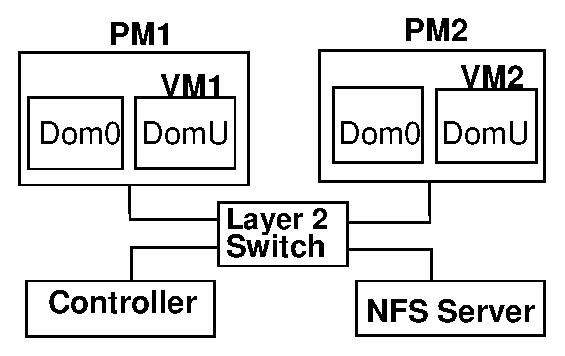
\includegraphics[scale=0.695]{jss-figures/benchmark}} 
~~~~~~~~~~~~~~~~~~~~
\subfloat[KVM setup]{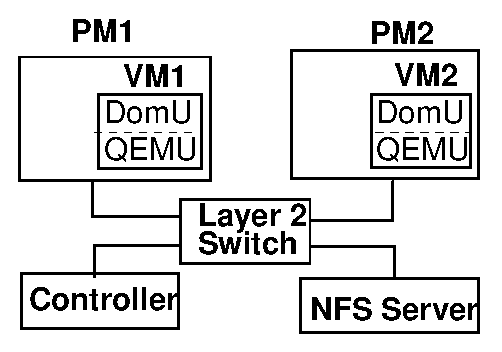
\includegraphics[scale=0.695]{jss-figures/kvmbenchmark}}
\caption{Setup for benchmarking, profiling and model evaluation.}
\label{fig:setup}
\end{figure}
Fig.~\ref{fig:setup} shows the experimental setup that we used. 
The setup used for benchmarking with Xen virtualization technology
is as shown in Fig.\ref{fig:setup}(a) wherein Dom0 is the privileged
domain as described earlier in Section~\ref{sec:litreviewchap-io-virtualization}. 
In case of KVM platform, 
there is no management domain since it
does not follow the driver domain I/O model. Hence, the setup
for KVM benchmarking is a slightly modified version, as
depicted in Fig.~\ref{fig:setup}(b).

As shown in the setup of Fig.~\ref{fig:setup}, two PMs (both with same 
configurations) host the VMs. Each PM
is connected via a Layer-2 Switch to an NFS server which hosts
disk images associated with the VMs. Thus, all disk read/write
operations are NFS-read/write operations which generate network traffic
at the host. The Controller is responsible
for coordination of load generation and resource-usage measurements 
on the VMs.
Load generation is done using an automated script residing at the Controller,
that invokes a custom application program (called \texttt{LoadGen})
at each VM.
For logging of resource utilization, we adopt the ``black-box''
approach~\cite{sandpiper}, i.e, we monitor VM's resource usage by measuring 
only at the hosts (PMs) and not inside the VMs.
% and not within the VMs themselves.
Resource utilization logging is done on the host, using utilities like
\texttt{sar}~\cite{sar}, \texttt{Xentop}~\cite{xentop} (for Xen), 
\texttt{top}~\cite{top} (for KVM) and 
\texttt{iptables}~\cite{iptables}.

The two physical machines hosting the VMs are Intel Core 2
Quad (Q9550) machines with 2.83 GHz cores. Xen version is
3.2 with Linux kernel 2.6.24-26 and KVM version is kvm-62
having QEMU PC emulator version 0.9.1.
%  and are dual-booting
% with Xen 3.2 virtualization environment and KVM module installed in Linux
% kernel version 2.6.24-26.
Both Controller and NFS server (not virtualized, hence common to 
both Xen and KVM setups) are Intel Core 2 (E7400) machines with 
2.60 GHz cores.
The Layer-2 Switch and all network links of the
machines operate at 100 Mbps.


\subsection{Workload generation}
\label{sec:arescue-workloadgen}
As part of our experimental evaluation, we generate 
different types of workloads for benchmarking and
model building.
Workloads are generated using a generic client-server setup,
wherein a \textit{client}
(the controller machine) remotely connects to 
the \textit{servers} (each PM or Dom0,
and VM or DomU). % where workload is to be generated. 
The workload generation
tool resides on each such ``server'' and complies with the 
load generation
requests received from the ``client'' machine. 
Referring to Fig.~\ref{fig:setup}, the 
workload generation requests are sent by the ``Controller''
and VM1/VM2 execute benchmarks to generate the 
requested resource utilization levels. 

Though more detail regarding the design, implementation
and usage of the load generation tool (called \texttt{LoadGen})
is presented in Appendix~\ref{chap:thesis-loadgen}, here 
we mention the different workloads briefly.
The different types of workloads generated by \texttt{LoadGen} are,
% 
% \textbf{SSS:Write up about micro-benchmarks. Also, mention
% the exponential number of cases to consider for combinational loads, and hence
% the randomized choice of combinational load cases.}
\begin{itemize}
\item \textbf{CPU-intensive workloads.}
CPU intensive workloads are generated by having a worker
thread calculate a Fibonacci series with varying periodicity.
If $T$ is the average time for a round of Fibonacci series calculation,
CPU load of $X\%$ is generated by having the worker thread perform
computations for $X \times T$ milliseconds (\emph{active period}) and
sleep for ($100-X) \times T$ milliseconds (\emph{sleep period}).
\item \textbf{Mutable and immutable network-intensive workloads.} 
We generate various levels of network traffic between a pair of VMs by using
a TCP-based custom application that sends a string of bytes on a
TCP socket with different periodicity.
For network workloads, we assume the maximum available capacity 
to be $100$ Mbps and vary the load on each VM by steps 
of $10$ Mbps, from $10$ to $90$ Mbps.
\item \textbf{Disk read \& write workloads.}
We generate disk read (or write) workload by reading (or writing) files  
of $4 kB$ size, with varying intervals to achieve different read access
rates ranging from 0 to 1280 blocks/second. Translating into Kbps, these
rates range from 0 to 5120 Kbps.
\item \textbf{Combination workloads.}
Combination or mixed workloads are generated using 
the same procedures as described above, with a 
multi-threaded process executing different workloads 
simultaneously.
\end{itemize}
As part of the experimental setup, we ensured that for each 
experiment, all combinations of workloads over all VMs do not 
saturate capacity of any resource, i.e., CPU utilization and 
I/O utilization levels are always less than 100\% in all experiments.

\subsection{Effect of colocation on CPU usage}
In this section, we empirically observe the effect of colocation
on CPU resource usages of both Dom0 and DomU. 
By design, we generate the ``same'' load (type and 
amount) for each experiment in both the configurations\textemdash{}dispersed and 
colocated\textemdash{}and observe the differences in actual resource utilization
levels. 
We are interested in addressing the following questions,
(i) For mutable network workloads, is there a decrease in CPU usage when
VMs are colocated, as compared to when they are dispersed? 
(ii) For pure CPU-intensive workloads, is the colocated Dom0 CPU usage
a simple summation of the individual (or dispersed) Dom0 usages, (iii) For
disk read \& write workloads, and immutable network workloads, is
the resultant colocated CPU usage a summation of usages in dispersed
scenarios?

%\begin{figure}%
%\hspace{-0.3in}
%\subfloat[DomU CPU utilization for Rx]{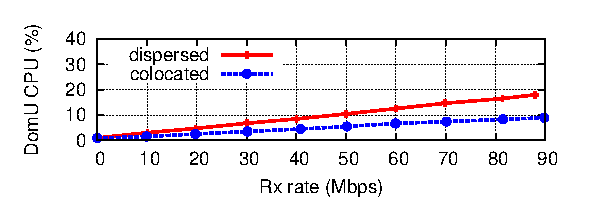
\includegraphics[scale=0.9]{arescue-figures/aff-benchmark/domU-cpu-vs-affine-rx-curve.eps}}
%\subfloat[DomU CPU utilization for Tx]{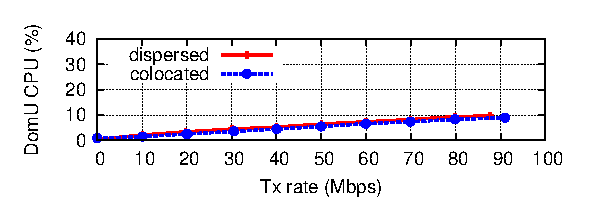
\includegraphics[scale=0.9]{arescue-figures/aff-benchmark/domU-cpu-vs-affine-tx-curve.eps}} \\
%\centering
%\subfloat[Dom0 CPU utilization for Rx/Tx]{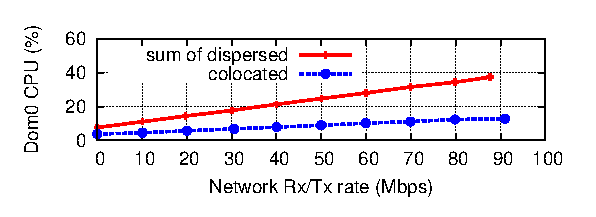
\includegraphics[scale=0.9]{arescue-figures/aff-benchmark/dom0-cpu-vs-affine-curve.eps}}%
%\caption{CPU utilization due to intra-PM network traffic (in Xen setup).}
%\label{fig:cpuovhd-rxtx}
%\end{figure}

%from 2ndchap-benchmark.tex
\begin{figure}[t]%
	% \centering
	\hspace{-0.3in}
	\subfloat[Dispersed DomU CPU utilization for Tx]{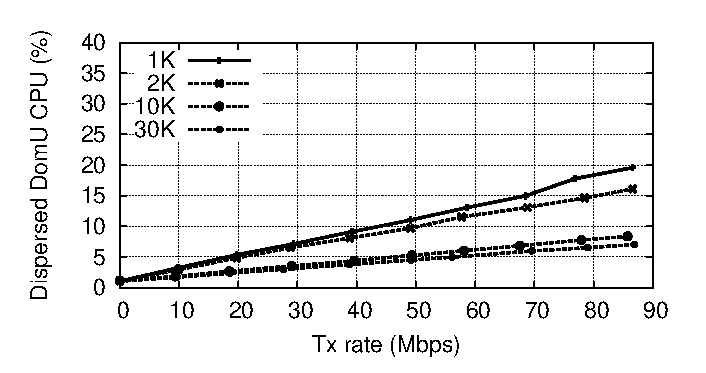
\includegraphics[scale=0.75]{jss-figures/new-aff-benchmark/domu-disp-cpu-for-tx-diff-file-sizes-notsoboth.eps}} ~~
	\subfloat[Colocated DomU CPU utilization for Tx]{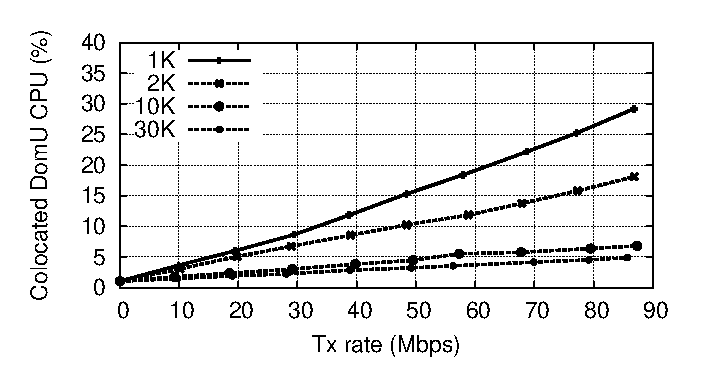
\includegraphics[scale=0.75]{jss-figures/new-aff-benchmark/domu-colo-cpu-for-tx-diff-file-sizes-notsoboth.eps}}
	\caption{CPU utilization due to mutable transmit traffic in dispersed and colocated scenarios with different segment sizes (in Xen setup).}
	\label{fig:xendomutx-chunks}
\end{figure}

\begin{figure}%
	% \centering
	\hspace{-0.3in}
	\subfloat[Dispersed DomU CPU utilization for Rx]{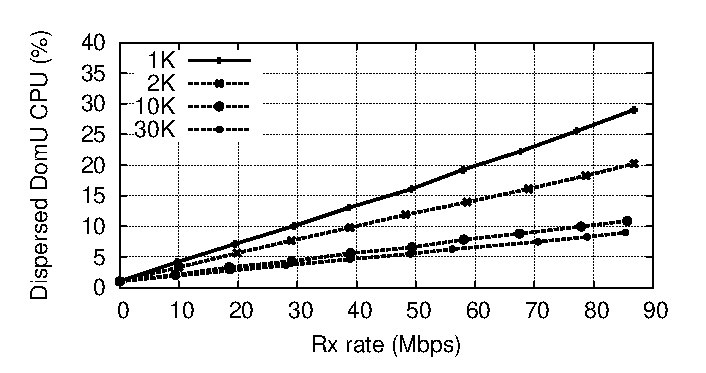
\includegraphics[scale=0.75]{jss-figures/new-aff-benchmark/domu-disp-cpu-for-rx-diff-file-sizes-notsoboth.eps}} ~~
	\subfloat[Colocated DomU CPU utilization for Rx]{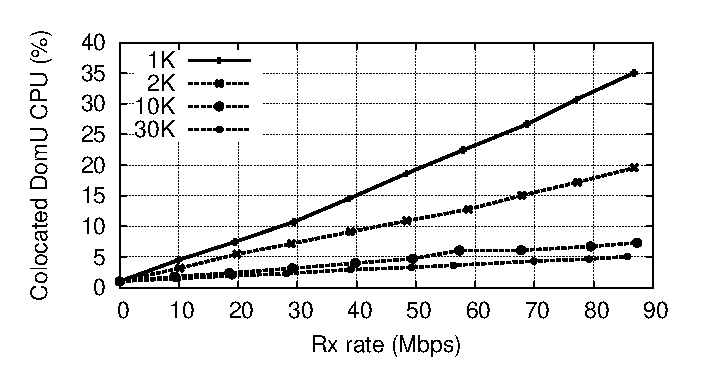
\includegraphics[scale=0.75]{jss-figures/new-aff-benchmark/domu-colo-cpu-for-rx-diff-file-sizes-notsoboth.eps}}
	\caption{CPU utilization due to mutable receive traffic in dispersed and colocated scenarios with different segment sizes (in Xen setup).}
	\label{fig:xendomurx-chunks}
\end{figure}

\begin{figure}[t]
	% \centering
	\hspace{-0.3in}
	\subfloat[Dispersed summation Dom0 CPU utilization for Rx/Tx]{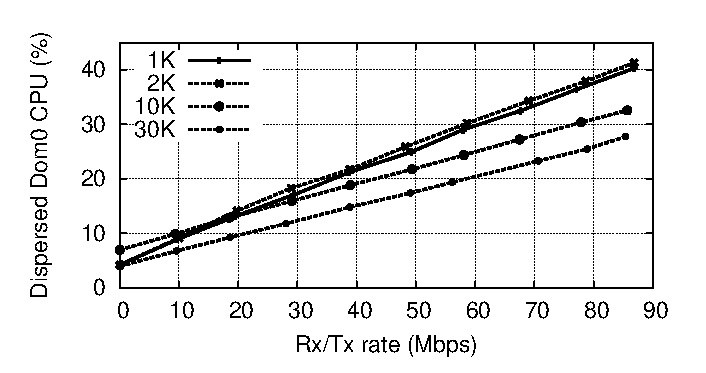
\includegraphics[scale=0.75]{jss-figures/new-aff-benchmark/dom0-dispsum-cpu-for-rxtx-diff-file-sizes-notsoboth.eps}} ~~
	\subfloat[Colocated Dom0 CPU utilization for Rx/Tx]{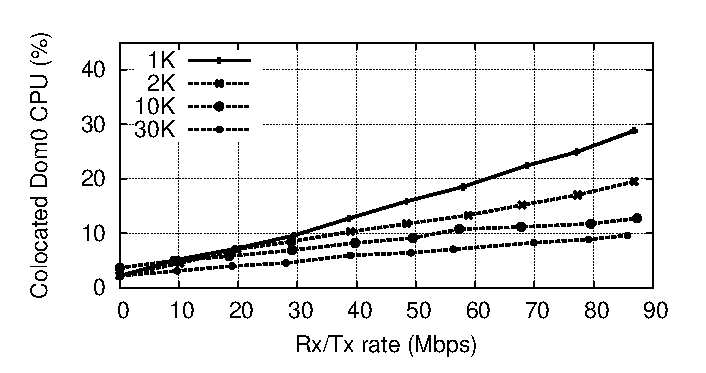
\includegraphics[scale=0.75]{jss-figures/new-aff-benchmark/dom0-colo-cpu-for-rxtx-diff-file-sizes-notsoboth.eps}}
	\caption{CPU utilization for mutable network traffic with different segment sizes (in Xen setup).}
	\label{fig:dom0rxtx}
\end{figure}

\paragraph{I. Impact of mutable network traffic in Xen.} 
One of our claims (and as also discussed 
in~\cite{virtual-putty}, \cite{starling}),
is that colocated provisioning can result in changes in
resource usage for mutually communicating VMs. % and availability. 
% `Affine' traffic refers to the network communication
% within the VM pair under consideration.
In this experiment, VM1
and VM2 act as a Tx/Rx pair to transmit and receive data
at different rates, such that
VM1 is the transmitting DomU\index{DomU}
and VM2 is the receiving DomU.
To study the implications of mutable network-affinity
between VMs, the experiment is conducted in both 
colocated and dispersed scenarios, and CPU utilization for
DomU (and Dom0 in Xen) is measured.
In our setup, we observed that TSO (TCP Segmentation
Offload)\nomenclature{TSO:}{TCP Segmentation Offload}\index{TSO} feature was
enabled whereas the complementary feature LRO (Large
Receive Offload)\nomenclature{LRO:}{Large Receive Offload}\index{LRO} at
receiving end
was not functional. For the sake of
uniformity at both transmitting and receiving ends, we disabled
TSO for our experiments.

Fig.~\ref{fig:xendomutx-chunks}(a) and \ref{fig:xendomutx-chunks}(b)
plot the transmitting DomU's CPU utilization for varying usage
of network bandwidth in Xen\index{Xen} setup. Each line represents
the use of a different application-level segment size
(sizes are mentioned in the legend).
As described in Section~\ref{sec:arescue-background}, inter-PM and
intra-PM communication have different execution paths,
hence resulting in different CPU utilization.
As can be seen, for higher segment sizes, increase
in network bandwidth usage results in higher CPU savings upon
colocation. However, the opposite result is
observed for smaller segment sizes.
The bold lines in the graph represent those
segment sizes for which colocated CPU usage is higher than
dispersed whereas the dotted lines indicate those having
colocated CPU usage as lower than dispersed. For example,
for the segment size of 30KB at 80Mbps network utilization,
CPU utilization is 8\% for dispersed and 4.8\% for colocated,
thus indicating a drop of approximately 3\% absolute CPU
when transitioning into colocated. On the other other hand,
for the segment size of 1KB at 85Mbps, CPU utilization
is 29\% for dispersed and 35\% for the colocated scenario,
which indicates a 6\% increase while moving into colocated placement.
A similar result was observed for the receiving DomU as well,
as depicted in Fig.~\ref{fig:xendomurx-chunks}.

Fig.~\ref{fig:dom0rxtx} shows Dom0 CPU utilization
levels for two communicating VMs,
with
\ref{fig:dom0rxtx}(a)
showing the summation of the two dispersed Dom0 CPU utilization
and
\ref{fig:dom0rxtx}(b)
showing the colocated Dom0 utilization.
We can see that in all cases,
the summation utilization is significantly greater than the
colocated Dom0 utilization. For example,
for the segment size of 30KB at 80Mbps network utilization,
the difference in absolute Dom0 CPU usage between
dispersed (summation of utilization at both Dom0's in the
dispersed scenario) and colocated (single
Dom0 CPU) scenarios is 16\% and similarly for 2KB segment size,
this difference is around 20\% absolute CPU.
The above observations suggest that not only the bit-rate of
transmission, but also the segment size affects CPU utilization
in both colocated and dispersed scenarios, and we need to consider
both these factors while modeling CPU usage. Further, we also
observe that in all above experiments, CPU usage varies linearly
with respect to network utilization.


% This implies that there is definitely
% no increase in CPU utilization due to colocation of two 
% communicating VMs.
%Further, the absolute usage by Rx-network traffic is more
%than Tx-traffic for the same bandwidth\textemdash{}CPU utilization
%of 17\% and 9\% respectively, at 90 Mbps network bandwidth
%utilization.
%Fig.~\ref{fig:cpuovhd-rxtx}(c) shows the Dom0 CPU utilization
%levels for two communicating VMs.
%Comparing network rates of 40 Mbps and 90 Mbps,
%the difference in absolute Dom0 CPU usage between
%dispersed (summation of utilization levels at both PMs in the
%dispersed scenario) and colocated (single
%Dom0 CPU) scenarios is 14\% and 25\%, respectively.

%when both the Rx/Tx network traffic is between colocated VMs.
%Considering network utilization of 85 Mbps, Dom0's CPU
%requirements is about 12\%.
%{\bf Dom0 plot should have dom0-non-co-hosted-rx as well. 
%the colocated scenario is plotting dom0-cpu-rxtx ... ?}

\begin{figure*}[t]%
	\centering
	\subfloat[Dispersed Guest VM CPU utilization for Rx]{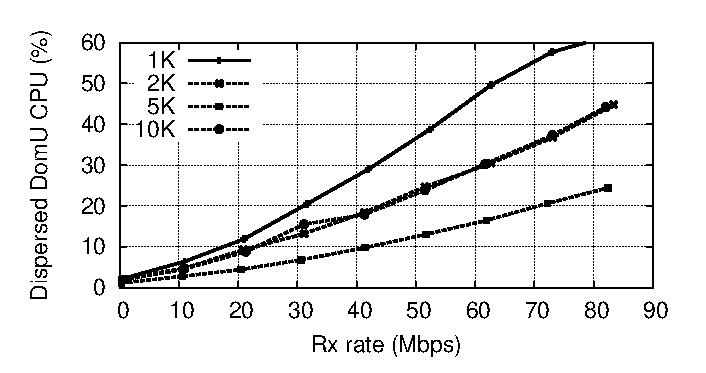
\includegraphics[scale=0.75]{jss-figures/kvm-aff-benchmark/domu-disp-cpu-for-rx-diff-file-sizes-notsoboth-kvm.eps}} ~~
	\subfloat[Colocated Guest VM CPU utilization for Rx]{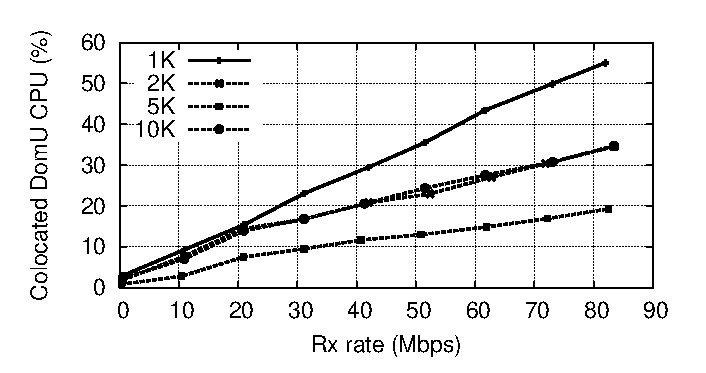
\includegraphics[scale=0.75]{jss-figures/kvm-aff-benchmark/domu-colo-cpu-for-rx-diff-file-sizes-notsoboth-kvm.eps}}
	\caption{CPU utilization for mutable receive traffic with different segment sizes (in KVM setup).}
	\label{fig:kvmdomurx-chunks}
\end{figure*}

\begin{figure*}[t]%
	\centering
	\subfloat[Dispersed Guest VM CPU utilization for Tx]{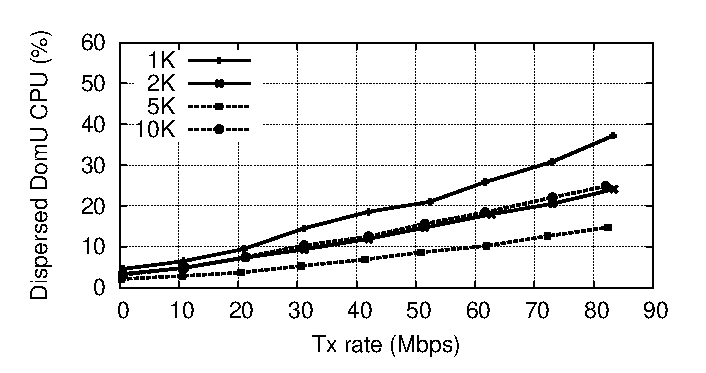
\includegraphics[scale=0.75]{jss-figures/kvm-aff-benchmark/domu-disp-cpu-for-tx-diff-file-sizes-notsoboth-kvm.eps}} ~~
	\subfloat[Colocated Guest VM CPU utilization for Tx]{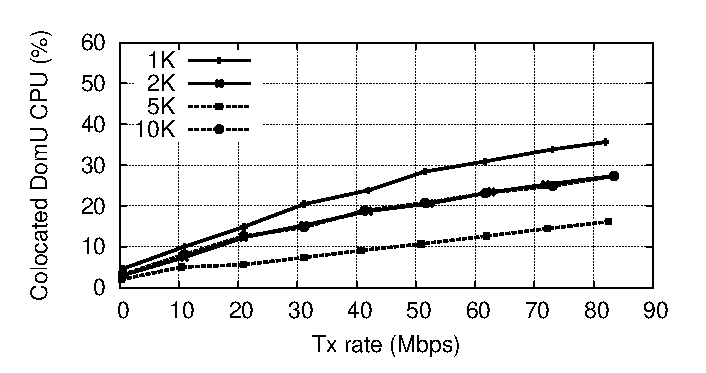
\includegraphics[scale=0.75]{jss-figures/kvm-aff-benchmark/domu-colo-cpu-for-tx-diff-file-sizes-notsoboth-kvm.eps}}
	\caption{CPU utilization for mutable transmit traffic with different segment sizes (in KVM setup).}
	\label{fig:kvmdomutx-chunks}
\end{figure*}

\paragraph{II. Impact of mutable network traffic in KVM.}
\label{sec:2ndchap-kvm-benchmark}
Similar to the benchmarking for Xen presented above, we performed
an empirical study of colocation effects in KVM as well.
As mentioned earlier, KVM does not have the concept of a privileged
domain to arbitrate I/O access amongst the VMs. Instead, each VM
is similar to a process and invokes the QEMU\index{QEMU} emulator to
access the
I/O devices. Thus, the overhead related to I/O processing (and the
resulting effects due to dispersed and colocated network
communication) would be reflected in the VM (DomU) CPU usage itself.
Fig.~\ref{fig:kvmdomurx-chunks} and Fig.~\ref{fig:kvmdomutx-chunks}
show CPU utilization
of the DomUs in dispersed and colocated scenarios in KVM\index{KVM}
setup. The experiment setting is such that VM1 requests varying
network rates in the range 10 to 80Mbps for
% (when VM1 requests, it plays
% the receiving domain role and VM2 is the transmitting domain) 
each segment size while VM2 requests a fixed rate of 10Mbps.
Thus, though both VMs are transmitting and
receiving data, the variations in network rate at a given
segment size setting are caused only by VM1's request-rate.

Fig.~\ref{fig:kvmdomurx-chunks} shows that when receive traffic
at VM1 is 80Mbps for a segment size of 10KB, DomU CPU usage is
44\% absolute CPU in dispersed case and drops to 35\% in colocated case
whereas for segment size of 1KB, CPU usage drops from 62\% in
dispersed case to 55\% in colocated case. Similarly,
Fig.~\ref{fig:kvmdomutx-chunks}
shows CPU usage plots for VM2 transmitting 80Mbps using
%the transmitting domain for 
various
segment sizes. Thus, we observe that CPU usage of transmitting
and receiving DomUs change between colocated \& dispersed scenarios.
Additionally, we also observe that CPU utilization
is approximately linear with respect to network utilization in
above experiments.


%%%%%%%%%%%%%%%%%%%%%%%%% nonaff-rx
\begin{table}
\caption{Percentage CPU usage for \textit{immutable} Rx.}
\centering
% \noindent\makebox[\textwidth]{% 
\begin{tabular}{|c|c|c|} \hline
\textbf{Immutable} & \multicolumn{2}{|c|}{\textbf{Percentage CPU utilization}} \\ \cline{2-3} \cline{2-3}
\textbf{Receive} & \textbf{Dispersed case} & \textbf{Colocated case} \\
(Mbps) & $VM_1,VM_2, \sum Dom0_i$ & $VM_1,VM_2,Dom0$ \\ \hline
% $<$20, 10$>$ & 3, 2, 12 & 3, 2, ~8 \\ \hline
% $<$20, 30$>$ & 4, 5, 14 & 3, 5, 11 \\ \hline
$<$20, 50$>$ & 4, 7, 18 & 4, 7, 14 \\ \hline
$<$20, 70$>$ & 4, 9, 21 & 4, 9, 17 \\ \hline
$<$40, 10$>$ & 6, 2, 15 & 6, 2, 11 \\ \hline
$<$40, 30$>$ & 7, 5, 18 & 7, 5, 15 \\ \hline
$<$40, 50$>$ & 7, 7, 21 & 7, 7, 18 \\ \hline
$<$60, 10$>$ & 8, 2, 18 & 8, 2, 14 \\ \hline
% $<$60, 30$>$ & 8, 5, 21 & 8, 5, 18 \\ \hline
\end{tabular}
% }
%\caption{Non-affine receive benchmarking results for colocated provisioning}
\label{nonaff-rx-benchmark}
%\vspace{-0.3in}
\end{table}

\paragraph{III. Other workloads.}
Table~\ref{nonaff-rx-benchmark} shows colocated benchmarking
results for immutable \textit{receive} traffic\textemdash{}VMs receiving 
network packets from ``dispersed'' (i.e. hosted on different PMs) transmitters. 
The table shows CPU usage of VMs in
dispersed and colocated cases for Dom0 and DomU.
The left most column shows tuples of the form $<x,y>$ where
$x$ is the the receive rate at VM1 and $y$ is the receive
rate at VM2. The second column shows the CPU utilization of 
VM1, VM2 and the summation of the CPU utilization of the two 
Dom0 instances in dispersed scenario. The third column shows
the CPU utilization of VM1, VM2 and the single Dom0 instance
in the colocated scenario.
Observe that
DomU CPU utilization stay similar in both dispersed \& colocated
cases.
The colocated Dom0
CPU utilization is consistently (4\%) less than 
the summation of the Dom0 utilization
levels in the dispersed case.

Similar observation was made for other workloads\textemdash{}immutable
transmit traffic, CPU workloads, disk read and disk write workloads. 
The Dom0 utilization of 4\% is the same as its utilization
under idle load, hence the above observation implies that for all
other workloads except mutable traffic, colocation results in saving
the CPU overhead related to an extra Dom0 instance.
%More detailed results can be found in the related technical report 
%at \cite{affine-modeling-tech-report}.

\paragraph{IV. Summary of benchmarking}
From the benchmarking phase, we have following take-aways,
\begin{itemize}
  \item When the nature of mutable network traffic changes between intra-PM
				  and inter-PM, there
				  is a change in guest VM CPU utilization in both Xen
				  and KVM environments. 
				  %, and this change is dependent on not only the
%				  network rate but also the application segment size.
  \item In case of Xen Dom0, change in nature of network-affinity results
				  in significant change (up to 25\% absolute CPU) when comparing
				  colocated Dom0 against the summation of dispersed Dom0 utilization.
  \item With increase in network utilization, 
	  the increase in CPU utilization is linear
			 in both Xen and KVM environments.
	\item For all workloads, other than mutable network traffic, colocation results
		in similar DomU CPU usages in both colocated and dispersed cases.
	\item For all workloads, other than mutable network traffic, the summation of CPU 
		usage of the two Dom0 instances in dispersed case differs from the 
		colocated CPU usage by a constant amount (say 4\% absolute CPU). 
\end{itemize}
		  
\textit{Based on the results of benchmarking, we
			  conclude that the relation between increase in network utilization
		  and CPU utilization is linear for both Xen and KVM environments.}
		  \footnote{These results are applicable only when both the network
			  and CPU resources have spare capacity, e.g., if CPU utilization is
			  already close to 100\%, increasing the network rate is either not
			  possible or results in no corresponding change in CPU utilization.
			  All further observations, modeling and inferences are based on this
		  premise.} As a result, both the ``total'' as well as 
		  the ``differences'' in CPU utilization can be
		  captured using linear estimation models.


%\paragraph{III. Summary of Xen benchmarking with colocation.}
%From the above set of benchmarking experiments, 
%we conclude that 
%For mutable network traffic, there is
%marginal reduction in DomU CPU utilization after colocation and
%significant savings (up to 25\%) in Dom0 CPU utilization.

%clipped 10feb
\subsection{Feasibility of Generic models}
In order to build a model that can be generically used to
predict CPU utilization of DomUs, 
even though it is trained on only one or couple of VMs,
it is necessary that VMs behave similarly under
similar loading conditions. 
For example, suppose a CPU load of
$x\%$ is requested, but creates $x+5\%$ CPU load on one VM.
%As mentioned before, this accuracy is enough for our benchmark
%profiling, however, 
It is essential that the same load when
requested on another homogeneous VM, results in similar
resource utilization levels. 
% This is a very basic expectation
% % and we present some sample results to demonstrate that this
% % does indeed hold. 
Thus, we are interested in verifying the 
following two hypotheses\textemdash{}(i) Given similar 
configurations, CPU utilization for similar load levels on 
different VMs match up, (ii) Given similar platforms, CPU 
utilization for similar loads on same VM but different PMs match up.
 
To this end, we performed several repeatable experiments 
on two VMs that were placed in a dispersed manner and compared whether 
similar loads result in similar CPU utilization levels on both VMs
and their Dom0s. We performed such experiments for all load 
types\textemdash{}CPU intensive, mutable traffic, immutable traffic
and disk-intensive\textemdash{}and as expected, we observed that both the
above hypotheses about CPU utilization on different VMs 
and PMs held true.
\\
\\
In this section, we established the basic benchmarking results that
will be applied to develop a generic CPU estimation model. By generic,
we imply that a single model would be able to estimate CPU utilization
for any given application, without requiring re-training on the specific
application itself.
In the next section, we present our approach to develop the generic
model and use it to estimate the CPU usage when a pair
of VMs are colocated or dispersed.



%\section{Our Approach: A-RESCUE}
\section{Linear regression modeling for CPU requirement estimation}
\label{sec:arescue-our-approach}


This section presents the core idea of our model generation and usage methodology.
%As mentioned earlier, our interest is to build a model that can capture the
%relationship between the resource utilization profiles and resultant CPU
%utilization when a pair of VMs transition from being dispersed to colocated,
%or vice versa.
We run a set of benchmarks, also referred to as micro-benchmarks, in both 
scenarios\textemdash{}dispersed and colocated\textemdash{}which exercise the utilization 
levels of VMs along different
axes\textemdash{}CPU, mutable and immutable network traffic, disk read and
write operations.


 \begin{table}
 \caption{Metrics considered per load type on each DomU (for predicting total CPU).}
%  \hspace{-0.2in}
 \begin{center}
 \begin{tabular}{|l|c|c|l|} \hline
  \bf{Disk} & \bf{Mutable} & \bf{Immutable} & \bf{CPU} \\ 
 & \bf{network} & \bf{network} & \\
  & \bf{traffic} & \bf{traffic} & \\ \hline
  Read (bytes/s) & Rx (Kbps) & Rx (Kbps) & User (\%) \\
  Write (bytes/s) & Tx (Kbps) & Tx (Kbps) & System (\%) \\
  Read (blocks/s) &  &  & Iowait (\%) \\
  Write (blocks/s) & &  & \\ \hline
 % Write blocks/sec & (NA) Tx Kbps & (A) Tx Kbps & System CPU\% \\
 %  &  &  & Iowait \\ \hline
 \end{tabular}
 \label{metrics-table}
 \end{center}
 \end{table}

\underline{Colocation and Dispersion models}: We wish to 
develop pair-wise CPU estimation models
that can predict total CPU requirement in target scenario
based on source scenario's resource usages.
Specifically, using resource usage measurements in
dispersed scenario, the ``colocation''
model predicts CPU utilization for VMs in the colocated scenario,
while the ``dispersion''
model uses resource usage measurements in the colocated scenario and 
predicts CPU utilization of VMs in the dispersed scenario.

Our benchmarking revealed that only the mutable network usage
causes change in CPU usage, upon change in VM placement.
Hence, we employ \underline{two approaches of prediction}:-
(i)~Predict \textit{total} CPU requirement based on multiple
resource usage profiles\textemdash{}CPU, disk and network,
(ii)~Predict \textit{differential} CPU requirement based only on
mutable network traffic metrics\textemdash{}later, take summation
of prediction with the source scenario's CPU usage to estimate
the total CPU requirement.
Next, we explain both approaches in detail.

\subsection{Approach 1: Prediction of total CPU requirement}

\paragraph{Core Idea: } Using the profiling data from 
execution of micro-benchmarks and strengthened
by our conclusions in Section~\ref{sec:arescue-benchmark}, we 
believe that a generic linear model to estimate 
\textit{total} (dispersed or colocated) CPU resource usage
is realizable. 
The total CPU requirement of a virtual machine accounts for all its
activities, including usage of all other resources. Hence, the model
for predicting total CPU requirement has all resource metrics as its
parameters: (i)~$4$ metrics for mutable and
immutable transmit and receive network rates (in Kbps),
(ii)~$3$ CPU metrics of \texttt{iowait}, \texttt{system}
and \texttt{user} CPU (in \%), and
(iii)~$4$ metrics among disk read/write rates in
blocks/second and bytes/second. These metrics are
tabulated in Table~\ref{metrics-table}.
Since the correlation of all resource usages to CPU usage is linear, we employ
linear regression methods to build the models for CPU estimation.

\paragraph{Micro-benchmark Profiling: } The idea is to capture 
behaviour of resource usage in all possible conditions
for both dispersed and colocated scenarios. So, the micro-benchmarks
should span the full range of resource utilization levels. 
The workload micro-benchmarks are generated using the workload
generation procedures described in Section~\ref{sec:arescue-workloadgen}.
For CPU micro-benchmarking, we split the CPU load on each VM
into $nine$ different intensities
ranging from $10\%$ to $90\%$. 
For network loads, we vary the load on each VM by steps 
of 10 Mbps, from 10 to 90 Mbps.
For disk read and write
micro-benchmarking, we vary the disk read/write rate from 
0 to 1280 blocks/second on each VM.

% Next, we describe briefly
% the approach adopted to ensure that we representatively
% cover the full range of resource utilization levels.

%For our profiling step, we use a generic client-server setup (described
%in more detail in Section~\ref{fig:setup}), wherein a \textit{client}
%(the controller machine) remotely connects to 
%the \textit{servers} (each PM or Dom0,
%and VM or DomU). % where workload is to be generated. 
%The workload generation
%tool resides on each such ``server'' and complies with the 
%load generation
%requests received from the ``client'' machine.
% 
% \textbf{SSS:Write up about micro-benchmarks. Also, mention
% the exponential number of cases to consider for combinational loads, and hence
% the randomized choice of combinational load cases.}

%clipped 10 feb
% \begin{itemize}
% \item \textbf{CPU micro-benchmark.}
% For CPU micro-benchmarking, we split the CPU load 
% into $nine$ different intensities
% ranging from $10\%$ to $90\%$. At each of the two VMs, 
% we vary the CPU load from $10\%$ to $90\%$, thus 
% resulting in $9 \times 9 = 81$ CPU workload
% combinations, as input for the modeling process.
% 
% \item \textbf{Network micro-benchmark.} 
% For network loads, we assume the maximum available capacity 
% to be $100Mbps$ and vary the load on each VM by steps 
% of $10Mbps$, from $10$ to $90 Mbps$.
% 
% \item \textbf{Disk read \& write micro-benchmarks.}
% For disk read and write
% micro-benchmarking, we vary the disk read/write rate from 
% 0 - 1280 blocks/second on each VM.
% For all files read and written, the block size is retained as $4 KB$.
% \end{itemize}


The set of inputs to train/build the models also includes 
combination workload benchmarks, which have CPU, network and disk
loads executed simultaneously, with different combinations of 
utilization levels.
However, to conduct exhaustive experiments that cover the
entire combination input set is not possible, since there is an
exponential number of cases in the input space of combinational load.
Thus, we adopted a workaround of choosing a set of random input 
workload levels. 
For each combination benchmark, we sample a target utilization level, for 
each workload type, from a pre-defined range\textemdash{}CPU utilization from $10\%$ to 
$90\%$, network rate from 10 Mbps to 90 Mbps and disk read/write rate
of $0$ - $1280$ blocks/second. Each sample for a workload type is chosen
uniformly at random. 
This is intended to keep the sample points
uniformly distributed throughout the available sample space. 

Overall, for the model building, we used 956 sample points in total, consisting
of 200 points for CPU workload, 96 points for mutable network usage, 182 points
for immutable network usage, 162 points for disk read workload, 158 points for disk write 
workload and 158 combinational workloads.
% Thus, a combinational load input to a single VM would
% be a 6-tuple of the form,
% $<$\textit{c}$\%$, $a$ Mbps, $nrx$ Mbps, $ntx$ Mbps, $r$, \textit{w}$>$ \\ 
% where,
% $c$ is a random number in [1-100] for generating $c$\% CPU load,
% $a$ is a random number in [1-90] for generating $a~Mbps$ affine network
% receive traffic (correspondingly $a~Mbps$ transmit
% traffic at the other VM),
% $nrx$ is similarly random in [1-90] for generating non-affine network
% transmit traffic, 
% $ntx$ is random in [1-90] for generating non-affine network
% transmit traffic, 
% $r$ and $w$ are randomly chosen file read/write
% rates between 0 - 1280 blocks/second. Note that given a pair of VMs,
% the affine network traffic transmitted by one VM is the affine network
% traffic received by the other.



% \paragraph{Profiling Resource Usage:}
% We use the same setup as shown in Section~\ref{initial-benchmarking} (refer Fig.~\ref{f14})
% for the load generation and logging, described in this section. 

% \begin{table*}[t]
% \begin{center}
% \begin{tabular}{|l|l|l|l|} \hline
% Disk & Non-affine(NA) network & Affine(A) network & CPU \\ \hline
% Read req/sec & (NA) Rx Kbps & (A) Rx Kbps & CPU\% \\
% Write req/sec & (NA) Tx Kbps & (A) Tx Kbps & \\ \hline
% \end{tabular}
% \caption{Tabulation of metrics for black-box approach considered per load type on each DomU.}
% \label{blackbox-metrics-table}
% \end{center}
% \end{table*}

\paragraph{Multi-Linear Regression Modeling: }
Since the correlation of various resource usage metrics 
in the dispersed (colocated)
case to CPU utilization level in the colocated (dispersed) 
case emerged as approximately linear, we employ 
linear regression methods to build the models for CPU estimation.
Using values from the collected profiling data,
%a set of equations which represent the colocated CPU usage
the colocated CPU usage is represented as 
a linear function of the individually profiled resource metrics
in the corresponding dispersed scenario (i.e. dispersed scenario
stressed with the same workload),
and similarly dispersed CPU usage is represented as a linear function of 
the colocated resource usage metrics.
% Each such equation will be of the form as shown in Eqn. (\ref{mlr-eqn})
The relation between estimated CPU and resource parameters is shown
in Eqn. (\ref{mlr-eqn}).
\begin{equation}
\mbox{CPU}^{i}_{estimated} = C_{0} + C_{1} \times M^{i}_{1} + C_{2} \times M^{i}_{2} + ... + C_{m} \times M^{i}_{m}
\label{mlr-eqn}
\end{equation}
where, $i$ is an iterator over each experiment or sample point
to be considered in the modeling, $m$ is
the number of parameters being considered, $M^{i}_{j}$ is
the value of parameter $M_{j}$ collected in the benchmark experiment number
$i$, and $\mbox{CPU}^{i}_{estimated}$ is the CPU usage 
either after dispersion or after colocation of VMs.
% The models that estimate the colocated CPU usage are referred 
% to as \textit{forward} models while 
% those that estimate the dispersed CPU utilization from the 
% colocated resource usage metrics are referred to as 
% \textit{reverse} models.
% In a \textit{forward} model, Dom0 %and DomU CPU usages
% CPU savings
% with colocated provisioning are predicted based on
% resource usages of VMs in the dispersed placements.
% In case of a
% black-box model (both forward and reverse), $m = 11$, and 
%The parameters considered per VM are, (i) $4$ metrics for mutable and 
%immutable transmit and receive network rates (in Kbps), 
%(ii) $3$ CPU metrics of \texttt{iowait}, \texttt{system} 
%and \texttt{user} CPU (in \%), and 
%(iii) $4$ metrics among disk read/write rates in 
%blocks/second and bytes/second. 
There are $11$ metrics in all to be considered, as discussed 
earlier in Table~\ref{metrics-table}. 
Both the colocation and dispersion DomU models have all these $11$ parameters.
The Dom0 \textit{colocation} model is built
with the metrics of both DomUs, and hence has $22$ parameters. 
The Dom0 \textit{dispersion} model 
depends on only one DomU's metrics at a time, and hence has only $11$
parameters.
% just like the DomU model. 
This is because the dispersed Dom0's CPU usage intuitively
depends on the resource usage of only its own hosted DomU and 
not on the other DomU of the VM pair.

\subsection{Approach 2: Prediction of differential CPU requirement}
\paragraph{Core idea: }
The difference in CPU usage upon transition between
colocated and dispersed placements of a VM pair, depends only on the mutable
network affinity between them. Hence, the idea here is to predict only
the difference, and sum it with the original scenario's CPU usage, to
obtain the total CPU requirement.
Note that differential Dom0 CPU is the difference in CPU 
usage between that incurred for the single (colocated) Dom0 and
the summation of both (dispersed) Dom0.
The model parameters are bit-rates (in Kbps) and packet-rates (in packets 
per second) for both transmission (Tx) and reception (Rx), thus four parameters
in all: (i) Rx Kbps, (ii) Rx pkts/s, (iii) Tx Kbps, and (iv) Tx pkts/s. 

\paragraph{Modeling of differential CPU utilization: }
Since we predict only the difference in CPU usage, the total
CPU requirement of the migrating VM on the target can be computed
as the sum of the predicted value and the observed CPU usage on
the source PM. Formally, Eqn. (\ref{cpu-diff-eqn}) captures the
general notion of change in CPU usage ($\Delta\mbox{CPU}$)
while transitioning between colocated and dispersed scenarios.
\begin{equation}
	% \hspace{-0.3in}
	\Delta\mbox{CPU} = \mbox{CPU}^{scenario1} - \mbox{CPU}^{scenario2}
	\label{cpu-diff-eqn}
\end{equation}
where, scenario$\{1|2\}$ = $\{colocated|dispersed\}$.
In case of \textbf{Dom0's CPU usage}, colocated Dom0 CPU usage is incurred
for hosting both VMs whereas dispersed Dom0 usage levels are
on behalf of a single VM each. During transition from dispersed
(\textit{disp} in short) to colocated (\textit{colo} in short),
the change in Dom0 CPU is defined as the difference in CPU usage
between that incurred for the single (colocated) Dom0 and the
summation of both (dispersed) Dom0, as illustrated in
Eqn. (\ref{dom0-diff-eqn-fwd}).
%\hspace{-0.2in}
\begin{equation}
	% \hspace{-0.3in} \mbox{CPU}^{dom0}_{diff} = \mbox{CPU}^{{dom0}_{1}}_{dispersed} + \mbox{CPU}^{{dom0}_{2}}_{dispersed} - \mbox{CPU}^{dom0}_{colocated}
	% \hspace{-0.3in} 
	%\delta\mbox{Dom0CPU}^{colo} = \mbox{Dom0CPU}^{colo} - \displaystyle\sum\limits_{i=1,2}\mbox{Dom0CPU}^{disp}
	\Delta\mbox{CPU}^{colo}_{Dom0} = \mbox{CPU}^{colo}_{Dom0} - \displaystyle\sum\limits_{i=1,2}\mbox{CPU}^{disp}_{Dom0}
	\label{dom0-diff-eqn-fwd}
\end{equation}
Similarly, during transition from colocated to dispersed, change in
CPU usage for each Dom0 instance is,
\begin{equation}
	% \hspace{-0.2in} 
	\Delta\mbox{CPU}^{disp}_{Dom0} = \mbox{CPU}^{disp}_{Dom0} - \frac{\mbox{CPU}^{colo}_{Dom0}}{2} %\frac{{CPU}^{dom0}_{colocated}}{2} 
	\label{dom0-diff-eqn-rev}
\end{equation}
% where i = 1,2.
Here we use %$\frac{{CPU}^{dom0}_{colocated}}{2}$ 
$\mbox{CPU}^{colo}_{Dom0}$/2
% as an approximation of CPU usage incurred
% for a single VM within the colocated scenario. Intuitively, the Dom0
% CPU usage incurred per VM in a colocated setting is different than
% that incurred in a dispersed setting, when intra-PM traffic is involved.
% This is % in Eqn. (\ref{dom0-diff-eqn-rev}) 
since colocated Dom0 CPU usage
is incurred on behalf of both VMs whereas we wish to predict
dispersed Dom0 CPU usage incurred on behalf of only a single VM each.
So, we use $\mbox{CPU}^{colo}_{Dom0}$/2 as an approximation of CPU usage
incurred for a single VM within the colocated scenario.
% so that the difference between Dom0
% usage on behalf of each VM in colocated and dispersed cases can be computed.
In case of \textbf{DomU's CPU usage}, we define change
in CPU as shown in Eqn. (\ref{domu-diff-eqn}).
\begin{equation}
	\Delta\mbox{CPU}_{DomU} = \mbox{CPU}^{disp}_{DomU} - \mbox{CPU}^{colo}_{DomU}
	\label{domu-diff-eqn}
\end{equation}
Based on Eqn. (\ref{domu-diff-eqn}), the difference needs to
be added to or subtracted from the observed CPU usage depending upon
whether the VM's migration results in dispersion or colocation, respectively. 
Thus, DomU's
colocation and dispersion models are one and the same, since the
\textit{magnitude} of the difference in CPU usage is the same in both
directions.

Using values from the collected profiling data,
%a set of equations which represent the colocated CPU usage
difference in CPU usage is represented as a linear function of the
individually profiled network usage metrics in dispersed
scenario (i.e. dispersed scenario stressed with the same workload).
The relation between estimated CPU and resource parameters is the
same as shown earlier in Eqn.~\ref{mlr-eqn}, except that
the value being estimated is the difference in CPU usage
and not the total.
In case of DomU model, the CPU usage estimate is expectedly a
function of its own network usage rates and uses all these four
metrics in its model. Similarly, in the case of Dom0 colocation model,
colocated Dom0 CPU usage accounts for both the colocated DomUs
and hence should intuitively depend on four metrics each of
both the DomUs, i.e. eight metrics in total. However, given a VM pair
with only mutual network communication, the received traffic by one
VM is the transmitted
traffic by the other, hence metrics of one VM are in fact
duplicates of metrics of the other, albeit in a different
order. We discard the redundant columns, therefore even Dom0
model has only four parameters. Thus, each model can be represented as
\begin{equation}
	% \mbox{CPU}_{est} = C_{0} + C_{1} \times Aff^{Rx}_{MBps} + C_{2} \times Aff^{Tx}_{MBps} + Aff^{Rx}_{pps} + Aff^{Tx}_{pps}
	% \hspace{-0.3in} \mbox{CPU}_{est} = C_{0} + C_{1} Aff^{R}_{K} + C_{2} Aff^{T}_{K} + C_{3} Aff^{R}_{P} + C_{4} Aff^{T}_{P}
	%\begin{split}
	\hspace{-0.3in} \Delta\mbox{CPU}_{est} = C_{0} + C_{1} \mbox{MutRx}_{Kbps} + C_{2} \mbox{MutRx}_{p/s} \\ 
	+ C_{3} \mbox{MutTx}_{Kbps}  + C_{4} \mbox{MutTx}_{p/s}
	%\end{split}
	\label{mlr-eqn-2}
\end{equation}
 where, ``Mut'' represents mutable network traffic,
  superscripts Rx \& Tx represent receive \& transmit, and
  subscript p/s represents the units packets/second.
\\
\\
To solve for the $m+1$ coefficients $C_{k}$, a stepwise linear
regression approach can help to select the ``best'' set of parameters.
%, in a stepwise manner.
% that would result in the most optimal prediction for the given learning dataset. 
% Thus, a model is learnt based only on these selected set of metrics. 
The stepwise approach ensures that only significant parameters that influence 
the predicted value are part of the model~\cite{applied-regression-analysis}.
For our implementation, we use the
% LARS~\cite{lars} package %present in Python~\cite{python} 
Robustbase package~\cite{robustbase}, part of the R statistical computing
environment, for robust and stepwise linear regression.
The linear regression solver, takes as input $M^{i}_{j}$ values for the 
various workloads and outputs values of $C_{k}$ that 
best predict CPU utilization. The set of coefficients thus
derived is the model that describes the relation between the $k$ parameters
and the total or differential CPU usage.

\subsection{Applying the pair-wise models to multi-VM scenarios}
\label{sec:multi-vm}
In order to apply the pair-wise models to situations with multiple
VMs hosting different applications
that may have different number of communicating tiers, the
first step needed is to consider that in a multi-VM scenario,
a single VM migration step
can result in not only dispersion w.r.t one (or a few) VM(s), but
also in colocation w.r.t other VM(s).
%To be more specific, the models that we have constructed so far
%apply to a single pair of VMs at a time i.e., in a single VM
%migration step, either two dispersed
%VMs can get colocated or two colocated VMs can get dispersed.
%In order to apply this CPU usage model to a real multi-VM 
%scenario, we need to be able to predict the CPU utilization 
%even in a combined scenario, wherein 
Fig.~\ref{fig:forward-plus-reverse} illustrates the case where
a single VM is being dispersed from one VM and colocated with another.
%Note that the terms DomU and VM are used interchangeably
%in this description and figure. 
Suppose $VM1$, $VM2$ and $VM3$ host different tiers of a 3-tier application.
As can be seen, one VM migration can result in that VM ($VM2$ in
Fig.~\ref{fig:forward-plus-reverse}) being dispersed from one VM ($VM1$)
on the source PM and being colocated with another VM ($VM3$) on
the target PM.

%Further, a VM that is communicating with multiple
%colocated VMs would get dispersed from all of them due to a single
%migration step. 
In the general multi-VM scenario, any particular VM (say $VM_{x}$)
may have multiple communicating neighbors, each of them belonging to
exactly one of three sets, (i) \textit{affinity-at-source}
(ii) \textit{affinity-at-target}, and (iii) \textit{affinity-at-other}.
Migration of $VM_{x}$ will cause it to become dispersed from
its \textit{affinity-at-source} set and colocated with its
\textit{affinity-at-target} set.
We refer to this dual step of being dispersed from
\textit{affinity-at-source} set and being colocated with
\textit{affinity-at-target} set, as a \textit{combined transition}.
In this case, the CPU utilization of all VMs in the
\textit{affinity-at-source} \& \textit{affinity-at-target} sets and
the migrating VM itself are expected to change.
In fact, the \textit{colocation}
and the \textit{dispersion} transitions can be viewed as
special cases of the \textit{combined} transition, starring only 
two VMs, with the dispersion transition being the case where 
dispersion set on source PM is empty while the dispersion transition 
is the case with an empty set on target PM.
Our aim is to predict the resource usage of all affected VMs and PMs.

\begin{figure}[t]
	\centering
	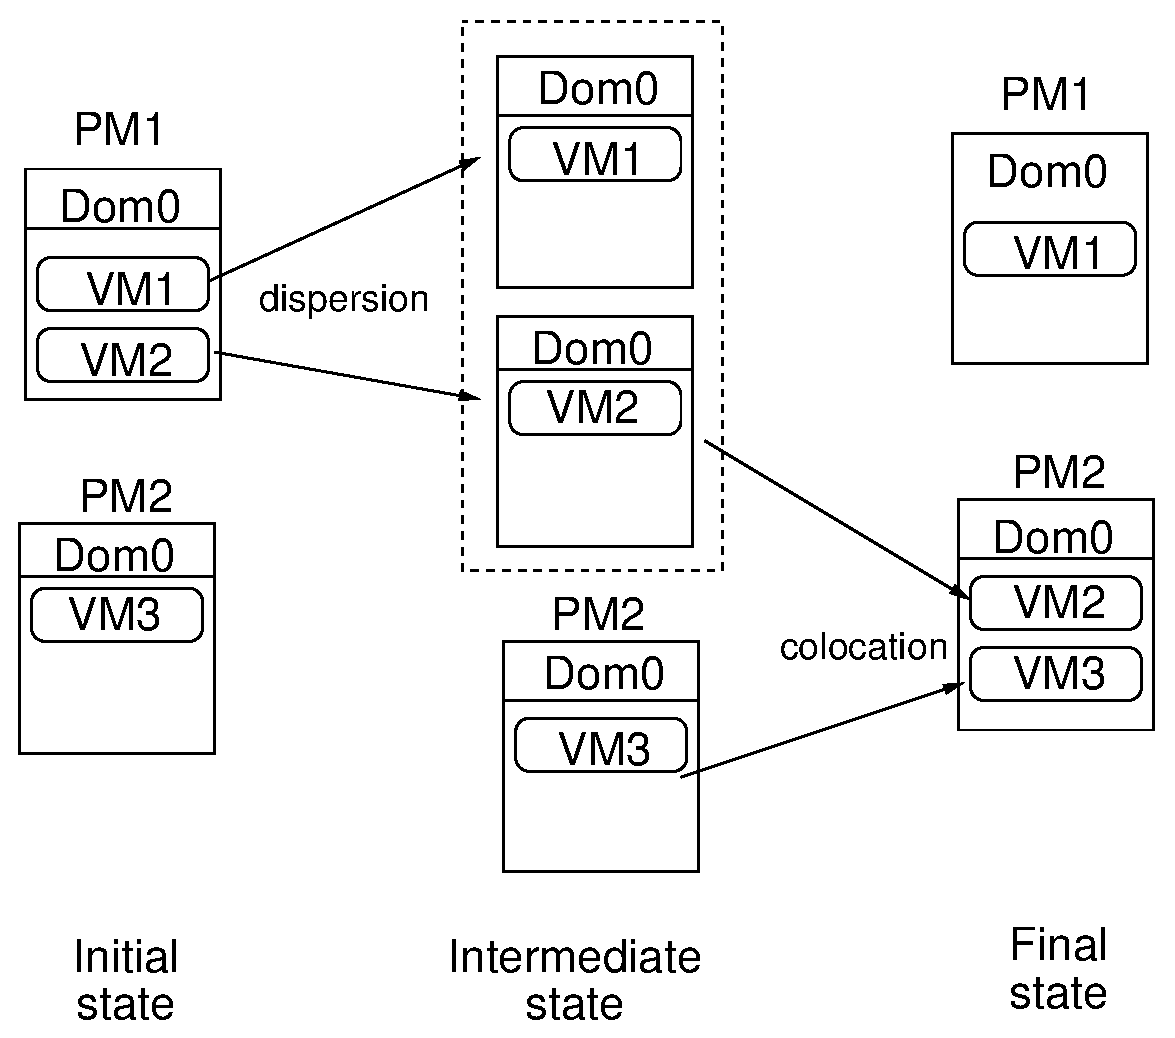
\includegraphics[scale=0.45]{jss-figures/new-forward-plus-rev.eps}
	\caption{Combined transition for $VM2$}
	\label{fig:forward-plus-reverse}
\end{figure}
% Our aim is to predict the CPU utilization when $VM2$'s migration
% causes a change in placement from \textit{Configuration1} to \textit{Configuration2}
% or vice versa. 

Consider the combined transition illustrated in Fig.~\ref{fig:forward-plus-reverse}.
It is straight-forward
to apply the DomU \textit{colocation} and \textit{dispersion} models to
$VM1$ and $VM3$ to predict their resultant CPU usages. Similarly, $PM1$'s
Dom0 CPU usage can also be predicted by applying Dom0 dispersion model.
However, prediction of $VM2$'s and $PM2$'s resultant CPU usage after this
combined transition needs a multi-phase prediction methodology.
The basic idea is to first apply the \textit{dispersion model} to the
measured metrics corresponding to network-affinity level between $VM2$
to/fro the \textit{affinity-at-source} set, and then use this
intermediate estimate
%This is an intermediate estimate and is used 
to make final prediction based upon network-affinity level
between $VM2$ to/fro the \textit{affinity-at-target} set. Incidentally,
VMs in the \textit{affinity-at-other} set do not affect $VM2$'s CPU
requirement because the nature of network-affinity
between them and $VM2$ is \textit{immutable} w.r.t its migration.
\\
\\
In this section, we described our model-building process and described
the synthetic training datasets used to learn this model.
We also described the process of applying the pair-wise prediction
models to multi-VM scenarios.
Though the models are built with synthetic datasets in which
TCP data-rates are generated by manipulating the application level
segment size and the periodicity of transmission, the application
scenarios for the models are not expected to have such controlled
behaviour. In particular, though the applications are
expected to use TCP for communication, the application-level
segment sizes and the inter-request times (also called think-times)
would be significantly more random. In the next section, we experimentally
evaluate the models on randomized synthetic data as well as on
benchmark application data. We also apply the model to multi-VM
scenarios and evaluate prediction effectiveness.


\section{Experimental evaluation}
\label{sec:arescue-experimental-eval}

%latest commented and above added for camera-ready
%\begin{figure}[t]
%\centering
%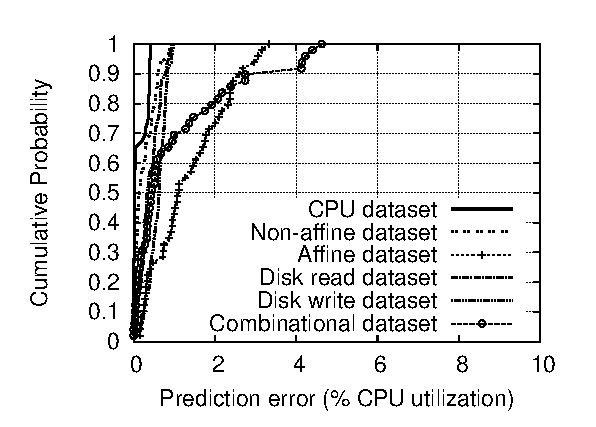
\includegraphics[scale=0.8]{synthetic-cdf-plots/dom0-forward-unseen-cdf.robust.eps}
%\caption{Prediction error CDF for \textit{colocated} Dom0 CPU estimation.}
%\label{fig:forward-unseen-cdf}
%\vspace{-0.25in}
%\end{figure}


In the previous section, we described the motivation and methodology
of developing models to predict colocated and 
dispersed CPU utilization.
After the models are built, we recompute or ``predict'' the colocated
CPU value for the training set itself, using the generated model 
coefficients. This is a sanity check to validate model correctness.
The results showed that well-fitting models 
were built, with less than 1\% to 2\% error for all workloads. However, the real test
is whether the models are able to successfully
predict the average CPU usage well, when applied to unseen data.
We present model evaluation on both synthetic data-sets and benchmark
application data in this section.


% 
% \begin{figure*}[t]
% \centering
% \noindent\makebox[\textwidth]{% 
% \begin{tabular} {cc}
% 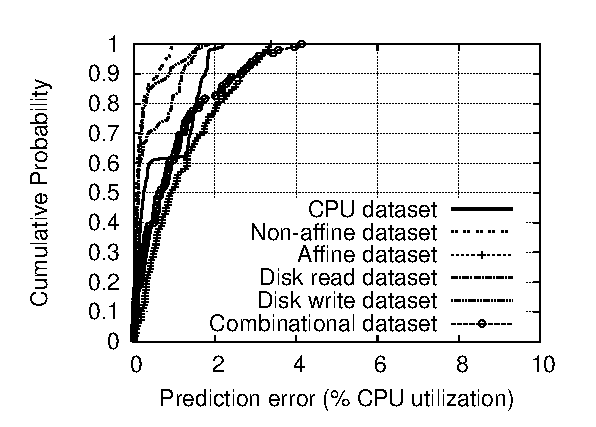
\includegraphics[scale=0.85]{synthetic-cdf-plots/domu-forward-unseen-cdf.robust.eps} & 
% 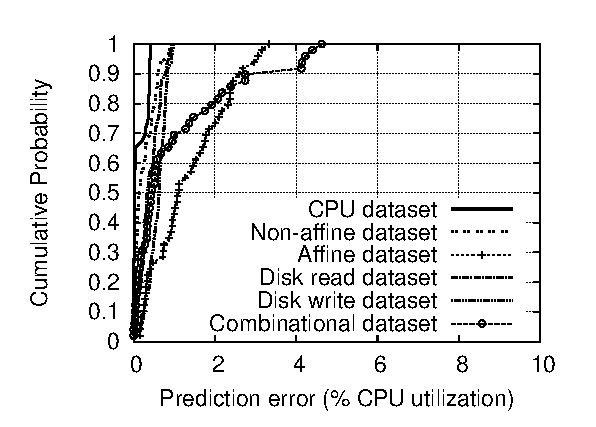
\includegraphics[scale=0.85]{synthetic-cdf-plots/dom0-forward-unseen-cdf.robust.eps} \\
% (a) DomU forward model & (b) Dom0 forward model 
% \end{tabular}
% }
% \caption{Prediction error CDF for \textit{colocated} CPU usage estimation.}
% \label{fig:reverse-unseen-cdf}
% \end{figure*}
% 
% 
% \begin{figure*}[t]
% \centering
% \noindent\makebox[\textwidth]{% 
% \begin{tabular} {cc}
% 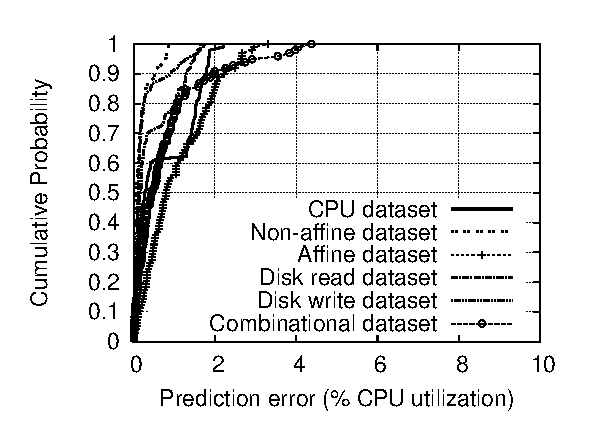
\includegraphics[scale=0.85]{synthetic-cdf-plots/domu-reverse-unseen-cdf.robust.eps} & 
% 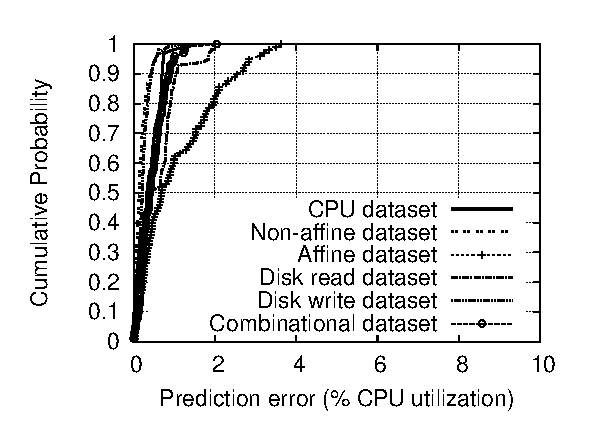
\includegraphics[scale=0.85]{synthetic-cdf-plots/dom0-reverse-unseen-cdf.robust.eps} \\
% (a) DomU reverse model & (b) Dom0 reverse model
% \end{tabular}
% }
% \caption{Prediction error CDF for \textit{dispersed} CPU usage estimation.}
% \label{fig:reverse-unseen-cdf}
% \end{figure*}

% \begin{figure*}[t]
% \centering
% \noindent\makebox[\textwidth]{% 
% \begin{tabular} {ccc}
% 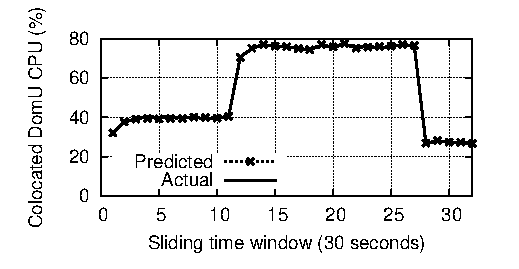
\includegraphics[scale=0.7]{aff-apps/rubis-co-domu1.eps} & 
% \includegraphics[scale=0.7]{aff-apps/rubis-co-domu2.eps} &
% 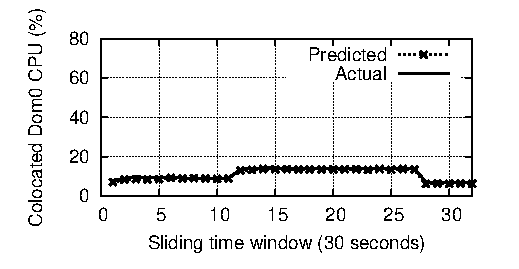
\includegraphics[scale=0.7]{aff-apps/rubis-co-dom0.eps} \\
% (a) Web tier VM & (b) DB tier VM &  (c) Colocated Dom0 \\
% \end{tabular}
% }
% \caption{Estimating colocated CPU utilization for RUBiS using \textit{forward} models.}
% \label{fig:rubis-forward}
% \end{figure*}



% \begin{figure*}[t]
% \centering
% \noindent\makebox[\textwidth]{% 
% \begin{tabular} {rccl}
% \includegraphics[scale=0.65]{aff-apps/rubis-dis-domu1.eps} &
% \includegraphics[scale=0.65]{aff-apps/rubis-dis-domu2.eps} &
% \includegraphics[scale=0.65]{aff-apps/rubis-dis-dom01.eps} &
% \includegraphics[scale=0.65]{aff-apps/rubis-dis-dom02.eps} \\
% (a) Web tier VM & (b) DB tier VM &
% (c) Dom0 of Web tier VM & (d) Dom0 of DB tier VM \\ 
% \end{tabular}
% }
% \caption{Estimating dispersed CPU utilization for RUBiS using \textit{reverse} models.}
% \label{fig:rubis-reverse}
% \end{figure*}


% \begin{figure*}[t]
% \centering
% \noindent\makebox[\textwidth]{% 
% \begin{tabular} {cc}
% \includegraphics[scale=0.65]{aff-apps/rubis-dis-domu1.eps} &
% \includegraphics[scale=0.65]{aff-apps/rubis-dis-domu2.eps} \\
% (a) Web tier VM & (b) DB tier VM \\ 
% \includegraphics[scale=0.65]{aff-apps/rubis-dis-dom01.eps} &
% \includegraphics[scale=0.65]{aff-apps/rubis-dis-dom02.eps} \\
% (c) Dom0 of Web tier VM & (d) Dom0 of DB tier VM \\ 
% \end{tabular}
% }
% \caption{Estimating dispersed CPU utilization for RUBiS using \textit{reverse} models.}
% \label{fig:rubis-reverse}
% \end{figure*}



\subsection{Model evaluation with synthetic data-sets}
In this sub-section, we present our findings when the generated
models were applied to ``unseen'' datasets. 
By unseen, we mean that these datasets are not a part of the
input set for model creation.
The setup used for evaluation with synthetic\index{Synthetic benchmarks} 
data-sets is the same 
as the one that was presented in Section \ref{sec:arescue-setup}, 
for the benchmarking experiments.
We present the evaluation of the two approaches separately\textemdash{}predicting
total CPU usage, and predicting differential CPU usage.

\begin{figure}[t]
% \centering
\hspace{-0.2in}
\subfloat[Dom0 CPU in colocated scenario (colocation model)]{\includegraphics[scale=0.9]{arescue-figures/synthetic-cdf-plots/dom0-forward-unseen-cdf-robust.eps}}
\subfloat[Dom0 CPU in dispersed scenario (dispersion model)]{\includegraphics[scale=0.9]{arescue-figures/synthetic-cdf-plots/dom0-reverse-unseen-cdf-robust.eps}}
\caption{Prediction error CDF for Dom0 CPU estimation.}
\label{fig:dom0-unseen-cdf}
% \vspace{-0.25in}
\end{figure}

% We test the models on the following workload types \textemdash{} CPU,
% intra-PM traffic, inter-PM traffic, disk read, disk
% write and also on combinational workloads.
\underline{For models predicting total CPU usage:}
The training data input for the models was generated
by generating resource utilization at pre-defined discrete 
levels, however, the derived models
need to be applied to ``unseen'' resource usage profiles
in order to judge their adequacy. For this reason, the
CPU workload for testing consists of $100$ randomly
picked values in the range $1\%$
to $100\%$, the mutable\index{Mutable} and immutable\index{Immutable} 
Rx/Tx test workloads
are chosen randomly from the range 10 Mbps to 90 Mbps, the
disk read/write rates are randomly chosen from the range
0 to 1280 blocks/second, and the combinational workloads 
had randomly chosen values for each parameter (CPU, mutable
network traffic, immutable network traffic,
and disk) from these same ranges.

Fig. \ref{fig:dom0-unseen-cdf} plots the CDFs of error when
Dom0 \emph{colocation} and \emph{dispersion} models were applied to all the
six unseen datasets\textemdash{}cpu, mutable \& immutable network traffic, disk read,
disk write and combinational loads. It can be observed that
all the CDFs seem to stick to the left end of the graph, however,
the 90th percentile
error is around 3\% absolute CPU and maximum error is around 4\%. 
We plotted similar error
CDFs for colocated and dispersed DomU CPU estimation. In 
all cases, we found that
the 90th percentile absolute error was within 3\%. We do
not present all the CDFs here, for sake of brevity; they can
be found in the technical report at \cite{affine-modeling-tech-report}.
In case of Dom0 models\index{Dom0 model}, 
since the savings due to co-location
is significant (as concluded from the benchmarking results), an
accuracy with 3\%error might suffice for a good prediction. However, in
case of DomU models\index{DomU model}, 
the savings themselves being marginally 
lower (between 0 to 10\%), a 3\% error could imply higher 
relative error in comparison. 
% With further increase in affine 
% network rate, increased CPU utilization (and hence increased 
% savings) may still benefit from this model's accuracy.
% \begin{figure*}[t]
% \centering
% \noindent\makebox[\textwidth]{% 
% \begin{tabular} {ccc}
% \includegraphics[scale=0.65]{figures/unseen-cpu-cdf.eps} & 
% \includegraphics[scale=0.65]{figures/unseen-aff-cdf.eps} &
% \includegraphics[scale=0.65]{figures/unseen-nonaff-cdf.eps} \\
% (a) CPU dataset & (b) Affine dataset &  (c) Non-affine dataset \\
% \end{tabular}
% }
% \caption{Prediction error CDF for different datasets.}
% \label{fig:forward-unseen-cdf}
% \end{figure*}

\begin{figure}[t]
	\hspace{-0.6in}
	\centering
	\subfloat[DomU-1]{\includegraphics[scale=0.95]{jss-figures/aff-synth/synth-co-domu1.eps}}
	\subfloat[DomU-2]{\includegraphics[scale=0.95]{jss-figures/aff-synth/synth-co-domu2.eps}} \\
	\subfloat[Colocated Dom0]{\includegraphics[scale=0.95]{jss-figures/aff-synth/synth-co-dom0.eps}}
\caption{Estimating colocated CPU utilization for synthetic data-set}% on Xen.}
\label{xensynth}
\end{figure}


\begin{figure}[t]
	\hspace{-0.6in}
	\centering
	\subfloat[Web tier VM]{\includegraphics[scale=0.95]{jss-figures/aff-apps/rubis-3way-co-domu1.eps}}
	\subfloat[DB tier VM]{\includegraphics[scale=0.95]{jss-figures/aff-apps/rubis-3way-co-domu2.eps}}
	\\
	\subfloat[Colocated Dom0]{\includegraphics[scale=0.95]{jss-figures/aff-apps/rubis-3way-co-dom0.eps}}
\caption{Estimating colocated CPU utilization for RUBiS} % using \textit{forward} models.}
\label{fig:2ndchap-rubis-forward}
\end{figure}

\underline{For models predicting differential CPU usage:}
In order to generate
synthetic workload which closely emulates a real application
scenario, we spawn multiple client processes, each sleeping
for fixed intervals of time (emulating average think-time)
and generating request for transmission of varying number
of bytes or segment sizes. Thus, the artificial constraint
of each client process requesting only a single segment size
has been discarded. We generate randomly different load levels
using different number of client threads every minute, each
generating requests for different segment sizes
and monitor resource usage utilization
over a period of 18 minutes. As expected,
the resultant network traffic rates and
CPU utilization also vary.

Fig.~\ref{xensynth} shows colocated\index{Colocated}
CPU usage, predicted versus actual, for both DomUs and Dom0.
We can see that as dispersed CPU utilization
changes due to change in network usage, predicted colocated
utilization also varies similarly.
% Fig.~\ref{xensynth-cdf} shows
% the prediction error CDFs for DomU and Dom0 forward and reverse models
% when applied to this synthetic data-set. 
The maximum error in DomU prediction is within 1\% absolute
CPU usage for both DomUs (VM1 and VM2) and the maximum
error in colocated Dom0 prediction is within 2.4\% absolute CPU.
Since difference in CPU utilization for DomU is
quite low and therefore less interesting, we focus on Dom0
models here onwards.


\subsection{Model evaluation with application benchmarks}
The above evaluation with synthetic workloads demonstrated
that predicting the differential CPU usage, which considers
only the mutable network usage metrics (including both network rate
and segment size metrics) give higher accuracy predictions.
Hence, we use that approach for the rest of the evaluation
in this chapter.


%\begin{figure}[t]
%\centering
%\subfloat[Web tier VM]{\includegraphics[scale=1]{../ieeecloud2011/savefigures/aff-apps/rubis-co-domu1.eps}} 
%\subfloat[DB tier VM]{\includegraphics[scale=1]{../ieeecloud2011/savefigures/aff-apps/rubis-co-domu2.eps}}  \\
%\subfloat[Colocated Dom0]{\includegraphics[scale=1]{../ieeecloud2011/savefigures/aff-apps/rubis-co-dom0.eps}}
%\caption{Estimating colocated CPU utilization for RUBiS using \textit{colocation} models.}
%\label{fig:rubis-forward}
%% \vspace{-0.25in}
%\end{figure}


For evaluating our prediction models with an application benchmark, we 
chose RUBiS~\cite{rubis}\index{RUBiS}.
RUBiS emulates an auction 
website like eBay, and allows simulation of various users/clients who engage
in different tasks like user registration, item registration, browsing items,
bidding for \& buying items and so on. 
RUBiS is a two-tier application, consisting of a web tier and a database tier
that communicate with each other for servicing each user request. Each tier
is hosted in a separate VM. 
We generate repeatable RUBiS workloads in both dispersed and colocated cases,
and compare average resource utilization levels (predicted versus measured)
over 30-second intervals. The RUBiS workload consisted of 800 clients
generating site browsing load simultaneously, and requests being fired
at determined times.
As done in~\cite{profiling-and-modeling}, we also consider open-loop
applications, where the inter-arrival times of the sequence of requests 
is the same across the dispersed and colocated scenarios. 
This is the case when response times are far lesser than the minimum
think-time. The think-times are randomly chosen from a negative 
exponential distribution with a mean of 7 seconds, and minimum think-time
of 5 seconds.

Fig.~\ref{fig:2ndchap-rubis-forward} plots predicted and measured CPU
utilization for the web tier VM (Fig. \ref{fig:2ndchap-rubis-forward}(a)),
the DB tier VM (Fig.~\ref{fig:2ndchap-rubis-forward}(b)) and the
Dom0 CPU utilization (Fig.~\ref{fig:2ndchap-rubis-forward}(c)) after colocation.
As seen in the figure, the RUBiS workload consists of 3 phases. It starts
with an
up-ramp phase which lasts till the 10th interval and then starts climbing
to steady state. Prediction is able to follow the climb well. The
steady state lasts till the 27th interval and then begins the ramp-down
phase. Prediction follows the drop also pretty accurately.
The maximum error in CPU
usage prediction is less than $2\%$ for both Dom0 and DomU models.
% When the VMs were moved from colocated to dispersed, the 90th percentile error
% in prediction was $3\%$ and $4\%$ for Dom0 and DomU models respectively.
Similar graphs were plotted for \emph{dispersion} model as well and
maximum error is within 2\% absolute CPU utilization.
Thus, prediction accuracies for both Dom0 and DomU models are equally high.
indicating that the models
can be successfully applied to an application without training on that
specific application's resource utilization profiles themselves.

\begin{table}[t]
	\centering
	\caption{Model accuracy with varying load}
	% \noindent\makebox[\textwidth]{%
	\begin{tabular}{|c|c|c|c|c|} \hline
		\textbf{No. of} & \textbf{Maximum}  & \multicolumn{3}{|c|}{\textbf{Max error (\% CPU)}} \\  \cline{3-5}
	\textbf{clients} & \textbf{net-affinity} & \textbf{DomU} &  \textbf{Dom0} & \textbf{Dom0} \\
		 & \textbf{(Mbps)} &  &  \textbf{colo} & \textbf{disp} \\ \hline  %\cline{2-9}
  500 & 6.8 & 1.73 & 1.33 & 0.90 \\
	1000 & 13.4 & 1.50 & 0.98 & 0.82 \\
	1500 & 19.8 & 1.42 & 0.69 & 0.90 \\
	2000 & 26.4 & 0.90 & 1.08  & 1.21 \\
	2500 & 32.6 & 1.03 & 1.29 & 1.27 \\
	3000 & 39.4 & 1.36 & 1.50 & 1.54 \\ \hline
	\end{tabular}
	% }
	\label{tab:xennumclients}
\end{table}


To demonstrate the extent of applicability of these models,
we conducted extensive experiments with various number of clients
in RUBiS and measured maximum error
in each case. This is tabulated in Table~\ref{tab:xennumclients},
where number of clients is increased
from 500 to 3000. We can see that in each case, maximum error
is within 2\% absolute CPU utilization.

\begin{table}
	\centering
	\caption{Model accuracy with varying network-affinity levels}
	% \noindent\makebox[\textwidth]{%
	\begin{tabular}{ |c|c|c|c|c|} \hline
		\textbf{No. of} & \textbf{Maximum} & \multicolumn{3}{|c|}{\textbf{Max error (\% CPU)}} \\ \cline{3-5}
		 \textbf{items} & \textbf{net-affinity} & \textbf{DomU} &  \textbf{Dom0 } & \textbf{Dom0 } \\
\textbf{per page} & \textbf{(Mbps)} &  & \textbf{colo} & \textbf{disp} \\ \hline
   5 & 4.8 & 1.51 & 1.55  & 1.06 \\
	 10 & 7.7 & 0.64 & 1.00 & 0.81 \\
	15 & 10.5 & 1.47 & 1.44  & 0.86 \\
	   20 & 13.4 & 1.5 & 0.98 & 0.82 \\
	   25 & 16.2 & 1.51 & 0.98  & 0.82 \\
	   35 & 21.5 & 1.27 & 1.02  & 0.87 \\
	   45 & 28 & 0.62 & 1.11  & 1.00 \\ \hline
	\end{tabular}
	% }
	\label{tab:xennumitems}
\end{table}

Another configurable parameter in RUBiS setup is the ``number
of items to be displayed per page'' %(\textit{NumItems}) 
for any
given browse or search request.
Within the RUBiS implementation, this parameter dictates the
network-affinity level between the web tier and the database tier.
At an abstract level, the amount of network data being sent per request
is similar to the concept of segment size considered earlier.
Thus, this parameter indirectly influences the range of
segment sizes that would be requested. The default value for
this parameter in RUBiS was 20, and though
this parameter would change very infrequently (or not at all) in a
production web service, we use this parameter as a knob to simulate
other web services which may have different network-affinity levels
with different segment sizes, flowing amongst its various tiers.
For the Xen-based RUBiS setup, we fixed number of clients to
2000 for this experiment and varied \textit{NumItems} from 5 to 45.
% We measured the 90 percentile error and the maximum error,
% listed in 
Table~\ref{tab:xennumitems} lists maximum prediction error
observed in each case\textemdash{}all within 2\%. %absolute CPU utilization.

\subsection{Estimating CPU usage for ``combined'' transitions}
\begin{figure}
	\centering
	\includegraphics[scale=0.425]{jss-figures/rubis-3tier-layout.eps}
	\caption{RUBiS 3-tier setup with proxy, webserver and database}
	\label{fig:threetier}
\end{figure}

In order to evaluate our prediction models on this combined transition,
we setup a three-tier application. Instead of using an existing three-tier
application, we use a simpler alternative of having an extra proxy
tier in the previous setup such that all client requests are
sent to this redirecting proxy, which forwards them on to the
web-server and also relays back the responses received from the
web-server back to the client. Fig.~\ref{fig:threetier}
is a pictorial representation of our
three-tier setup, where we use Muffin\cite{muffin} proxy
as the first tier of our test application.

\begin{figure}[h]
	\centering
	\includegraphics[scale=0.8]{jss-figures/aff-3tier/fwd_3tier_dom0_cdf.eps}
	\caption{Error CDF of Dom0 CPU estimation for C1 to C2 transitions}
	\label{fig:combined}
\end{figure}

\underline{Prediction for two configurations:} The RUBiS\index{RUBiS} 
application run is then performed in
two configurations\textemdash{}(i) \textit{C1}: with proxy server (VM1)
and web-server (VM2) colocated
on PM1 while database server (VM3) hosted alone on PM2, and
(ii) \textit{C2}: with VM1
hosted alone on PM1 while VM2 and VM3 are colocated on PM2.
Resource usage monitoring is performed on both PMs, as before.
Fig.\ref{fig:combined} shows the CDF of prediction error
considering error in prediction for all three PMs, during transition
from \textit{C1} to \textit{C2} and vice-versa.
Maximum error is within 1\% absolute CPU usage for both transitions.

\begin{figure}
	\centering
	\subfloat[\textit{C0}]{\includegraphics[scale=0.475]{jss-figures/rubis-3tier-alone.eps}} ~~~~~~~~~
	\subfloat[\textit{C1}]{\includegraphics[scale=0.475]{jss-figures/rubis-3tier-diff.eps}} \\
	\subfloat[\textit{C2}]{\includegraphics[scale=0.475]{jss-figures/rubis-3tier-same.eps}} ~~~~~~~~~
	\subfloat[\textit{C3}]{\includegraphics[scale=0.475]{jss-figures/rubis-3tier-alone.eps}}
	\caption{Different placements due to series of VM migration steps.}
	\label{fig:migration-steps}
\end{figure}



\underline{Prediction over series of migration steps:}
The above experiment demonstrated that \textit{colocation} and
\textit{dispersion} models can be used as building blocks to do multi-phase
CPU usage prediction for combined transitions. To extend this
further, we consider a series of VM migration steps for this three-tier
application such that each VM migration step results in a different
VM placement and we apply \emph{colocation}\index{Colocation model} and
\emph{dispersion}\index{Dispersion model} prediction models
appropriately to derive CPU usage prediction for each step. The series
of VM migration steps being considered are (Fig.\ref{fig:migration-steps}
shows configurations): (a) \textit{C0}: all 3 VMs on different PMs each
(b) \textit{C1}: VM2 migrates into PM1 and is colocated with VM1
(c) \textit{C2}: VM2 migrates into PM3 and is colocated with VM2
(d) \textit{C3}: VM2 migrates into PM2, same as initial configuration.
For each of the above configurations, we measure CPU utilization
incurred for a RUBiS run with 1000 clients. To test our models, we perform
prediction of CPU usage for the three Dom0 instances (corresponding to
PM1, PM2 and PM3) upon transition from one configuration to the next (e.g.,
\textit{C0}$\rightarrow$\textit{C1},
\textit{C1}$\rightarrow$\textit{C2} and
\textit{C2}$\rightarrow$\textit{C3}).
Maximum error in prediction for each step is listed in
Table \ref{tab:vm-steps-error}.

\begin{table}[h]
	\centering
	\caption{Error in Dom0 prediction over series of VM migrations.}
	% \noindent\makebox[\textwidth]{%
	\begin{tabular}{ |c|c|c|c|} \hline
		\textbf{Transition} & \multicolumn{3}{|c|}{\textbf{Maximum error}} \\
		 & \multicolumn{3}{|c|}{\textbf{in Dom0 prediction}} \\
		 & \multicolumn{3}{|c|}{\textbf{(\% absolute CPU)}} \\ \cline{2-4}
		 & \textbf{PM1} & \textbf{PM2}  & \textbf{PM3} \\ \hline  %\cline{2-9}
		\textit{C0}$\rightarrow$\textit{C1} & 0.75 & NA & NA \\
		\textit{C1}$\rightarrow$\textit{C2} & 1.99 & NA & 0.85 \\
		\textit{C2}$\rightarrow$\textit{C3} & NA & 0.51 & 0.43  \\ \hline
	\end{tabular}
	% }
	\label{tab:vm-steps-error}
\end{table}



Table \ref{tab:vm-steps-error} shows that for every transition step,
Dom0 CPU prediction models perform good prediction and maximum
error is within 2\% absolute CPU utilization. The entry NA in any
particular column implies that prediction is not performed for that
PM during that step. This could be due to one of two reasons: (i) Due to
the VM migration step, the PM has become idle, or (ii) During the
VM migration step, the PM is not the source or destination of
migration.
Thus, we have demonstrated that simple CPU usage prediction models built
on the scale of two VMs can be extended to apply to multi-VM
scenarios as well.


%Though our empirical study is based on Xen virtual machine 
%monitor (VMM\index{VMM}), the approach
%is general enough to be applicable to other virtualization technologies as
%well. For example, in case of KVM\index{KVM} where there is no concept 
%of a privileged
%domain, we expect that the affinity related benefits will be more
%prominently visible in the VM's CPU usage itself, and the above-mentioned modeling will
%prove valuable for CPU usage prediction on colocation/dispersal. We set this
%aside for future work.






%Move related work into 2ndchap, since this chapter already has a background
%\section{Related Work}
%
The work in this paper is focused on effects of relative location
(colocation or dispersion) on the CPU utilization of communicating virtual
machines. 
% The effect of network-affinity on CPU usage has been 
% alluded to in past research. For example, in \cite{virtual-putty}, the authors
% claim that the decrease in physical network usage due to colocation will 
% eventually translate to an increase in another resource dimension, say CPU.
% However, no empirical studies have been presented to quantify it so far.
%Additionally, 
Though most server consolidation and load balancing algorithms 
\cite{capacity-management, sandpiper, autonomic-vm-placement} acknowledge
that VMs may have elastic resource requirements to satisfy dynamically
varying load levels, it is generally accepted that resource requirement
to support a single load level is the same on all homogeneous physical 
machines. In this work, we present an empirical study to quantify the effect 
of colocation on CPU utilization of mutually communicating VMs, and 
demonstrate that a single resource configuration to handle a certain 
load level is at-best not efficient and at-worst short of requirements.
Thus, our work is supplementary to many server consolidation and load 
balancing approaches proposed in literature so far, and hence we use 
this section to chronicle the related work in these areas.

\subsection{Server consolidation and load balancing} 
During periods of under-utilization, multiple virtual machines can
be migrated onto a single physical machine, such a step is referred
as \textit{Server Consolidation}. On the other hand, when load
experienced on a single physical machine increases such that resource
requirements exceed resource capacity, \textit{Hotspot Mitigation} is
performed by migrating out some of the virtual machines.
Thus, both the problems of server consolidation and hotspot mitigation are
enabled by virtual machine migration.
Given a set of VM configurations, the general problems of server consolidation
and hotspot mitigation are viewed as bin-packing problems, which are NP-Hard. 
Trace-based approaches \cite{capacity-management} have been adopted to 
predict workload and perform consolidation, whereas online monitoring
and reactive approaches \cite{sandpiper, autonomic-vm-placement} are used
to address problems of load balancing and hotspot mitigation. 

In all above efforts, 
VM configurations per load-level are assumed 
to be constant, implying that 
it is considered that a VM that requires $x$ \% of a resource
on a PM would need the same amount of that resource on another
homogeneous PM. Also, in most cases, CPU resource utilization 
levels determine whether the PM is heavily or under-loaded.
If the VMs under consideration are
mutually communicating, then this ``network affinity'' causes changes
in the CPU usage profiles depending on the neighborhood set of
colocated VMs and their communication patterns. Thus, in case of 
communicating VMs (or application tiers), it is essential to be
``affinity-aware'' while determining VM configurations, and the configurations
need to be recomputed each time, instead of being assumed constant.

\subsection{Affinity-aware provisioning}
% This section presents the recent work done in the area of affinity-aware VM placement.
% For communicating tiers of an application that are placed on dispersed VMs,
It has been demonstrated in \cite{virtual-putty} that
transfer time between two communicating VMs can be 
reduced drastically
(as much as 90\%) by placing both on the same host.
This points to opportunities for
server consolidation based on \textit{network affinity}. 
%Server consolidation based on network affinity 
This may not only
improve response or transfer times but also reduce the load on network
resources, since the inter-VM communication between VMs co-hosted on a
single physical machine is more akin to IPC rather than a network transfer.
% The authors suggest that co-location of VMs would reduce the network
% usage while increasing the CPU usage. This is contrary to our observations,
% presented in this paper, which show that for our $100Mbps$ network links,
% colocation need not always result in increased CPU usage.
The effect of network-affinity on CPU usage has been 
alluded to in past research. In \cite{virtual-putty}, the authors
claim that decrease in physical network usage due to colocation will 
eventually translate to an increase in another resource dimension, say CPU.
However, no empirical studies have been presented to quantify it so far,
and hence the benchmarking study presented in this thesis is especially relevant.

A non-intrusive black-box approach for identifying mutually communicating
groups of VMs or \emph{VM ensembles}, called Net-Cohort, is presented
in \cite{net-cohort}. 
This work advocates monitoring only guest-level network statistics 
using hypervisor-tools and building an N$\times$N correlation matrix
to ``infer'' network communication rather than ``observe'' it by 
explicit monitoring of network traffic between all VM pairs.
Using hierarchical clustering algorithm, VMs are grouped into 
ensembles based on correlation in their resource usage.
% using hierarchical clustering.
After this initial identification of potential mutually communicating VMs,
packet sniffing is performed only on those VMs to identify
the actual communication dependencies. This work is complementary to
our work, in that, it can provide the affinity relations 
between various VMs which are required for 
affinity-aware CPU utilization estimation at datacenter scale.
% requires affinity relations 
% between various VMs to be known/identified, which can be provided
% using the solutions proposed in \cite{net-cohort}.
%if it is more efficient than the 

% In a follow-up paper~\cite{starling}, the authors have 
% presented 
A decentralized affinity-aware migration technique, which
takes into consideration the network transmission traffic between
each VM pair and tries to minimize communication overhead in 
the entire cluster of VMs, is presented in \cite{starling}. 
The \textit{bartering algorithm} presented
in \cite{starling} reflects the basic assumption of similar
CPU requirements irrespective of VM placement. However, our work
suggests that this assumption may not hold in real scenarios and
network affinity-aware CPU requirement estimation is essential.

\subsection{Estimation of virtualized CPU usage}
\label{cpu-estimation-refs}
A set of micro-benchmarks are used to profile the CPU 
usage on a given hardware
platform, using regression modeling techniques 
in \thinspace\cite{profiling-and-modeling}. The aim is to 
determine the virtualization overheads of an
application before it is placed in a virtualization environment,
so that it is not accidentally deployed to a physical machine with
insufficient resources. This is useful during initial placement of
applications into the virtualized domain, also referred to as VM Sizing.

% Hussam Mousa et al.\thinspace\cite{characterizing-performance}
% also use a regression modeling approach to identify the cause of performance
% overhead in both physical and virtualized machine instances. Profiling
% is done per execution interval and each interval is a defined number
% of executed instructions. During each interval, events are collected from
% hardware performance monitoring counters (PMC), guest kernels and the
% Hypervisor. The work in \cite{characterizing-performance} lays stress on
% the importance of synchronizing and aligning the measurement intervals, so
% that linear regression models will be applicable to the collected data.

We borrow the idea of micro-benchmark profiling from this paper, however,
we apply it to solve the problem of estimating colocated (virtualized)
CPU usage given two dispersed (virtualized) resource usage profiles.
Additionally, consider the scenario that the VMs to be transitioned from 
physical to virtual are mutually
communicating VMs or form various tiers of a single application. 
Depending on whether communicating VMs are colocated or dispersed upon
transition from physical to virtual domain, their virtualized CPU overhead
and CPU usages would be different, and thus our work can help extend 
the work in \cite{profiling-and-modeling}.
% \\ \\
% In this Section, we presented a brief overview of related literature. In the
% next Sections, we define our problem statement and describe our solution
% approach.

\subsection{Note about applicability of linear regression models to other virtualization solutions}
Recently, there has been work on fast network virtualization 
stack (eg. Click OS~\cite{clickos}). 
ClickOS is basically a minimal VM based on Xen’s MiniOS. The network path is 
redesigned to achieve higher network rates, using strategies like a higher 
speed switch, directly mapped packets between the switch and network front-end 
driver inside the VM, and mapping of ring buffers into memory space of network 
front-end driver inside the VM. In such cases, CPU utilization of guest VMs 
will be proportional to the L2/L3 processing, which is traditionally handled 
by Dom0 (referring to Xen paravirtualization setup). 

Most of the evaluation in \cite{clickos} is related to throughput for 
different packet sizes, and doesn’t mention the CPU overheads related to 
I/O processing. In our work, we explicitly consider paravirtualization 
setups and observe linear correlation between network and CPU usage, whereas 
in other scenarios like HVMs and pass-through setups, some of the CPU 
overheads will need to be recalculated and implications may change. 
In general, benchmarking of CPU usage to network throughput relationship 
should be done before making any conclusions regarding whether the 
relationship is linear or not. 

However, as long as the optimization is such that it applies proportionally 
for various network throughput levels for a single packet size, a linear 
dependence between CPU utilization and network throughput may continue to 
hold. On the other hand, if the inter-VM path is optimized such that the 
CPU usage in inter-PM scenario is not much greater than in intra-PM scenario, 
then the difference in CPU usage between co-located and dispersed scenarios 
maybe insignificant and hence not need any modeling.

%\label{sec:arescue-related-work}

% %Keep related work here instead of in 2nd chapter
\section{Implications of affinity-aware CPU estimation}
\label{sec:arescue-related-work} 

The work in this paper is focused on effects of relative location
(colocation or dispersion) on the CPU utilization of communicating virtual
machines. 
% The effect of network-affinity on CPU usage has been 
% alluded to in past research. For example, in \cite{virtual-putty}, the authors
% claim that the decrease in physical network usage due to colocation will 
% eventually translate to an increase in another resource dimension, say CPU.
% However, no empirical studies have been presented to quantify it so far.
%Additionally, 
Though most server consolidation and load balancing algorithms 
\cite{capacity-management, sandpiper, autonomic-vm-placement} acknowledge
that VMs may have elastic resource requirements to satisfy dynamically
varying load levels, it is generally accepted that resource requirement
to support a single load level is the same on all homogeneous physical 
machines. In this work, we present an empirical study to quantify the effect 
of colocation on CPU utilization of mutually communicating VMs, and 
demonstrate that a single resource configuration to handle a certain 
load level is at-best not efficient and at-worst short of requirements.
Thus, our work is supplementary to many server consolidation and load 
balancing approaches proposed in literature so far, and hence we use 
this section to chronicle the related work in these areas.

\subsection{Server consolidation and load balancing} 
During periods of under-utilization, multiple virtual machines can
be migrated onto a single physical machine, such a step is referred
as \textit{Server Consolidation}. On the other hand, when load
experienced on a single physical machine increases such that resource
requirements exceed resource capacity, \textit{Hotspot Mitigation} is
performed by migrating out some of the virtual machines.
Thus, both the problems of server consolidation and hotspot mitigation are
enabled by virtual machine migration.
Given a set of VM configurations, the general problems of server consolidation
and hotspot mitigation are viewed as bin-packing problems, which are NP-Hard. 
Trace-based approaches \cite{capacity-management} have been adopted to 
predict workload and perform consolidation, whereas online monitoring
and reactive approaches \cite{sandpiper, autonomic-vm-placement} are used
to address problems of load balancing and hotspot mitigation. 

In all above efforts, 
VM configurations per load-level are assumed 
to be constant, implying that 
it is considered that a VM that requires $x$ \% of a resource
on a PM would need the same amount of that resource on another
homogeneous PM. Also, in most cases, CPU resource utilization 
levels determine whether the PM is heavily or under-loaded.
If the VMs under consideration are
mutually communicating, then this ``network affinity'' causes changes
in the CPU usage profiles depending on the neighborhood set of
colocated VMs and their communication patterns. Thus, in case of 
communicating VMs (or application tiers), it is essential to be
``affinity-aware'' while determining VM configurations, and the configurations
need to be recomputed each time, instead of being assumed constant.

\subsection{Affinity-aware provisioning}
% This section presents the recent work done in the area of affinity-aware VM placement.
% For communicating tiers of an application that are placed on dispersed VMs,
It has been demonstrated in \cite{virtual-putty} that
transfer time between two communicating VMs can be 
reduced drastically
(as much as 90\%) by placing both on the same host.
This points to opportunities for
server consolidation based on \textit{network affinity}. 
%Server consolidation based on network affinity 
This may not only
improve response or transfer times but also reduce the load on network
resources, since the inter-VM communication between VMs co-hosted on a
single physical machine is more akin to IPC rather than a network transfer.
% The authors suggest that co-location of VMs would reduce the network
% usage while increasing the CPU usage. This is contrary to our observations,
% presented in this paper, which show that for our $100Mbps$ network links,
% colocation need not always result in increased CPU usage.
The effect of network-affinity on CPU usage has been 
alluded to in past research. In \cite{virtual-putty}, the authors
claim that decrease in physical network usage due to colocation will 
eventually translate to an increase in another resource dimension, say CPU.
However, no empirical studies have been presented to quantify it so far,
and hence the benchmarking study presented in this thesis is especially relevant.

A non-intrusive black-box approach for identifying mutually communicating
groups of VMs or \emph{VM ensembles}, called Net-Cohort, is presented
in \cite{net-cohort}. 
This work advocates monitoring only guest-level network statistics 
using hypervisor-tools and building an N$\times$N correlation matrix
to ``infer'' network communication rather than ``observe'' it by 
explicit monitoring of network traffic between all VM pairs.
Using hierarchical clustering algorithm, VMs are grouped into 
ensembles based on correlation in their resource usage.
% using hierarchical clustering.
After this initial identification of potential mutually communicating VMs,
packet sniffing is performed only on those VMs to identify
the actual communication dependencies. This work is complementary to
our work, in that, it can provide the affinity relations 
between various VMs which are required for 
affinity-aware CPU utilization estimation at datacenter scale.
% requires affinity relations 
% between various VMs to be known/identified, which can be provided
% using the solutions proposed in \cite{net-cohort}.
%if it is more efficient than the 

% In a follow-up paper~\cite{starling}, the authors have 
% presented 
A decentralized affinity-aware migration technique, which
takes into consideration the network transmission traffic between
each VM pair and tries to minimize communication overhead in 
the entire cluster of VMs, is presented in \cite{starling}. 
The \textit{bartering algorithm} presented
in \cite{starling} reflects the basic assumption of similar
CPU requirements irrespective of VM placement. However, our work
suggests that this assumption may not hold in real scenarios and
network affinity-aware CPU requirement estimation is essential.

\subsection{Estimation of virtualized CPU usage}
\label{cpu-estimation-refs}
A set of micro-benchmarks are used to profile the CPU 
usage on a given hardware
platform, using regression modeling techniques 
in \thinspace\cite{profiling-and-modeling}. The aim is to 
determine the virtualization overheads of an
application before it is placed in a virtualization environment,
so that it is not accidentally deployed to a physical machine with
insufficient resources. This is useful during initial placement of
applications into the virtualized domain, also referred to as VM Sizing.

% Hussam Mousa et al.\thinspace\cite{characterizing-performance}
% also use a regression modeling approach to identify the cause of performance
% overhead in both physical and virtualized machine instances. Profiling
% is done per execution interval and each interval is a defined number
% of executed instructions. During each interval, events are collected from
% hardware performance monitoring counters (PMC), guest kernels and the
% Hypervisor. The work in \cite{characterizing-performance} lays stress on
% the importance of synchronizing and aligning the measurement intervals, so
% that linear regression models will be applicable to the collected data.

We borrow the idea of micro-benchmark profiling from this paper, however,
we apply it to solve the problem of estimating colocated (virtualized)
CPU usage given two dispersed (virtualized) resource usage profiles.
Additionally, consider the scenario that the VMs to be transitioned from 
physical to virtual are mutually
communicating VMs or form various tiers of a single application. 
Depending on whether communicating VMs are colocated or dispersed upon
transition from physical to virtual domain, their virtualized CPU overhead
and CPU usages would be different, and thus our work can help extend 
the work in \cite{profiling-and-modeling}.
% \\ \\
% In this Section, we presented a brief overview of related literature. In the
% next Sections, we define our problem statement and describe our solution
% approach.

\subsection{Note about applicability of linear regression models to other virtualization solutions}
Recently, there has been work on fast network virtualization 
stack (eg. Click OS~\cite{clickos}). 
ClickOS is basically a minimal VM based on Xen’s MiniOS. The network path is 
redesigned to achieve higher network rates, using strategies like a higher 
speed switch, directly mapped packets between the switch and network front-end 
driver inside the VM, and mapping of ring buffers into memory space of network 
front-end driver inside the VM. In such cases, CPU utilization of guest VMs 
will be proportional to the L2/L3 processing, which is traditionally handled 
by Dom0 (referring to Xen paravirtualization setup). 

Most of the evaluation in \cite{clickos} is related to throughput for 
different packet sizes, and doesn’t mention the CPU overheads related to 
I/O processing. In our work, we explicitly consider paravirtualization 
setups and observe linear correlation between network and CPU usage, whereas 
in other scenarios like HVMs and pass-through setups, some of the CPU 
overheads will need to be recalculated and implications may change. 
In general, benchmarking of CPU usage to network throughput relationship 
should be done before making any conclusions regarding whether the 
relationship is linear or not. 

However, as long as the optimization is such that it applies proportionally 
for various network throughput levels for a single packet size, a linear 
dependence between CPU utilization and network throughput may continue to 
hold. On the other hand, if the inter-VM path is optimized such that the 
CPU usage in inter-PM scenario is not much greater than in intra-PM scenario, 
then the difference in CPU usage between co-located and dispersed scenarios 
maybe insignificant and hence not need any modeling.



\section{Open directions}
\label{sec:arescue-open-directions}

% \subsection{Bench-marking CPU Utilization for UDP Affine Traffic}
% In this paper, we have focussed on server-type multi-tier applications
% which employ TCP communication across tiers. Our benchmarking experiments
% also spawned processes that opened TCP sockets and performed connection
% oriented communication. Here, we perform a brief experiment to observe
% the difference in CPU usage when UDP connectionless traffic is present 
% instead of TCP. Intuitively, the CPU usage would be higher due to the
% necessity of having to set up UDP socket for every datagram being sent
% across. In our custom UDP application, we use the same segment sizes
% as before, ranging from 1KB to 70KB and Fig.~\ref{udprx} presents the
% CPU utilization incurred at the receiving DomU in dispersed and
% colocated scenarios, respectively.


\subsection{Benchmarking of 1 Gbps link network usage}
\label{ref:1gbps}
In our experiments, we used network links with capacity 100 Mbps 
for network traffic
and found that CPU usage had a linear correlation with network usage.
This was the basis for using a linear regression modeling technique
for CPU estimation. However, in order for our approach to be valid
for 1 Gbps links, this linear correlation should hold in a setup with
traffic up to 1 Gbps as well. To this end, we performed a benchmarking
exercise as before (with Xen), but with a 1 Gbps link, to answer
the following questions:
%We perform this study for the Xen virtualization environment here.
%The motivations of this study are two-fold:-
(i) Does the linear correlation of CPU to network usage still hold 
with 1 Gbps links?
(ii) Does using different capacity links between communicating VMs 
result in different CPU utilization at the VMs (and Dom0 for Xen)?

\begin{figure}[t]
\centering
\includegraphics[scale=0.75]{jss-figures/new-aff-1G-benchmark/multi-bytetcp-1Gbps-nogsotsoboth-0iptabs-5120-dom0-cpu-vs-affine-curve.eps}
\caption{Dom0 Utilization over a 1Gbps link}
\label{fig:link1gbps}
\end{figure}



Fig.~\ref{fig:link1gbps} shows CPU utilization at Dom0
for network-affinity levels ranging from 100 to 900 Mbps, in 
both dispersed and colocated scenarios for segment size of
5KB. As can be seen, the CPU utilization is linearly correlated with
network rate in both the cases. 
% We made similar observations at the transmitting DomU as well. 
Thus, we conclude that 
linear regression modeling approach can be applied for affinity-aware
CPU estimation even in deployments with 1 Gbps links. However, 
the CPU utilization
incurred for network rates $\le$ 100 Mbps over a 1 Gbps link are not the 
same as those observed during benchmarking with 100 Mbps links. 
%More
%specifically, CPU required to transmit or receive 50Mbps traffic 
%over a 100Mbps link is not the same as that required over a 1Gbps link.
This implies that network link bandwidth is an important
determinant of CPU utilization incurred at the transmitter and
receiver. So, if the cloud deployment has networks links or switches 
of heterogeneous capacities,
different CPU estimation models would have to be
developed for each link type.

\subsection{Effect of colocation for data-centric applications}
The work in this paper is targeted towards multi-tiered service-oriented
applications such that the user issues a request and waits 
for a certain time (think-time) before firing the next request.
In such a scenario, where think-time intervals are relatively large
(as compared to response transmission time),
requests are issued at long enough intervals
such that observed network-affinity levels
in colocated and dispersed scenarios are the same. 
However, for data-centric applications 
where tiers exchange large amounts of data, the transmission
durations are significant and hence 
observed network-affinity levels in colocated
and dispersed placements are not same (for observation intervals
smaller than data transmission durations).
%Hence, performance of
%such applications would experience significant difference
%in colocated and dispersed scenarios. 
%For example, an 18 minute
%run of RUBiS workload would finish in 18 minutes in both 
%dispersed and colocated scenario. 
For example, with an application
that sends bulk data in an as-soon-as-possible manner, the 
completion time may be sooner or later depending
on whether the participating VMs are colocated or dispersed
and hence the network bandwidth available in each scenario. 
An enhanced model that estimates the network-affinity level 
and resulting CPU utilization based on placement scenarios would
be required.
%This 
%implies that 
%change in relative placement for VMs of a data-centric application
%would result in change in affine network traffic rates as well,
%and CPU utilization on the target would be a function
%of the network rate in the new placement scenario. Thus, an
%extra step of predicting the resultant affine network rate
%is also needed in this case.

\subsection{Capacity planning for virtualized services}
An important aspect of migration of services from physical to virtual
environments (P2V) is estimation of resources needed to meet SLA
requirements
\cite{migrating-n-tier-apps, migrating-service-oriented, 
legacy-app-migration}.
%A capacity planning exercise is needed the estimation of total 
%resources needed
%to migrate a set of applications from physical to virtual (P2V transition)
As shown in our work, colocation
and dispersion of communicating tiers of an application can
result in differing CPU utilization for both DomUs and Dom0.
Thus, estimating CPU usage of two tiers individually
for the P2V transition will neglect the effects of affinity 
on their CPU usage.

Resource requirement in virtualized
environment depends on type of application being migrated
from physical to virtual. 
In \cite{profiling-and-modeling}, linear regression models
have been built to estimate virtual CPU usage from given
physical resource usage profiles. However, this has been 
done only for one tier (web server tier) of the application
and not for the other (database tier). Thus, it 
does not
consider both cases\textemdash{}colocation and dispersion\textemdash{}of 
location of the two tiers, and instead addresses only the
dispersed placement by default. In our work, we have demonstrated that 
virtualized CPU usage of both communicating tiers are
dependent on their relative placement also. Thus, during
the P2V transition, virtual CPU usage estimation should
also consider whether or not the communicating VMs are intended
to be colocated. Our idea is that for every VM that has
network communication with any other VM, the P2V CPU estimation
models presented in \cite{profiling-and-modeling} can be
used to predict its dispersed virtual CPU usage, and then
our \textit{colocation} model can be applied to this estimation
to predict the final virtual CPU usage. 


% Note that, this
% transitive approach to P2V CPU usage prediction closely
% couples the VM's CPU usage and its placement.

% In \cite{migrating-n-tier-apps},
% change in performance upon migration of n-tier applications 
% to different clouds is addressed and the causes identified, 
% whereas \cite{migrating-service-oriented, legacy-app-migration} focus
% on the processes, methods and tools needed for this P2V transition.


\section{Conclusions}
\label{sec:arescue-conclusions}
In this work, we performed benchmarking, to
quantify the effects of network affinity on CPU usage when communicating VMs
are colocated versus dispersed.
Next, we developed VM \textit{pair-wise} models
that can estimate ``colocated'' CPU usage, on being
input their individual dispersed-case resource usages,
and to estimate ``dispersed'' CPU
usage based on colocated-case resource usages.
For the ``colocation'' and ``dispersion'' models, we first
built models that predicted the total CPU usage
upon migration\textemdash{}these CPU models used all resource (CPU, disk, mutable
and immutable network) usage profiles as their input. However, these models
had an error of around 4\%. So, next we built enhanced models
to predict only the differential CPU usage\textemdash{}these
models use only the \textit{mutable} network traffic metrics as input,
and have maximum error within 2\%. Finally, we demonstrated the
application of \textit{pair-wise} models to predict for multi-VM
scenarios, with high accuracy.
%We tried two approaches
%of modeling and found that predicting differential CPU usage provided
%better accuracy\textemdash{}with maximum error within 2\% absolute CPU usage.
%We also demonstrated that simple 
This proves that CPU usage prediction models built
on the scale of two VMs can be used for prediction in multi-VM
scenarios as well.


%In this work, we have empirically profiled different kinds of workloads and
%presented the effect of colocation on the DomU and Dom0 CPU utilization for Xen.
%We also presented models for estimation of the CPU usage when dispersed VMs
%are moved to colocated placement and vice-versa. 
%Experiments showed the 90 percentile error to
%be less than 3\% absolute of CPU utilization, over both synthetic and real
%application workloads.
%
%Though our empirical study is based on Xen virtual machine monitor, the approach
%is general enough to be applicable to other virtualization technologies as 
%well. For example, in case of KVM where there is no concept of a privileged
%domain, we expect that the affinity related benefits will be more 
%prominently visible in the VM's CPU usage itself, and the above-mentioned modeling will 
%prove valuable for CPU usage prediction on colocation/dispersal.
%
%In our work, we have made the assumption of homogeneity of PMs,
%both in terms of capacity as well as the architecture. 
%The assumption of homogeneity of capacity can be withdrawn provided the higher 
%level consolidation or placement algorithm accounts for the differing capacities
%and makes placement decisions accordingly. However, the assumption of homogeneity
%of architecture may be non-trivial to dispense with, because on such differing
%architectures, the Dom0 and DomU CPU usage may also
%be different and not directly mapped~\cite{profiling-and-modeling}. It would be of 
%interest to
%develop mappings from one architecture to another, so that our model can
%be extended to apply to machines with heterogeneous architectures as well.




%\part*{Network Communication aware CPU Usage Estimation for Virtualized Applications}
%\chapter{Affinity-aware Modeling of CPU usage for Provisioning Virtualized Services}\label{current-work-v2v}
%\chapter{A-RESCUE v1.0: \underline{A}ffinity-aware \underline{res}ource-based \underline{C}PU \underline{u}tilization \underline{e}stimation} 
%\chapter{Affinity-aware Modeling of CPU usage for Virtualized Applications}
%\label{chap:thesis-v2v-1}
%
\section{Introduction}

In traditional datacenters, the practice is to either follow
a dedicated model and provision servers for peak loads, or share
resources in a best-effort manner that offers no
guarantees~\cite{resource-overbooking}.
For example, an auction website may be hosted on a single PM
in order to guarantee that it has enough resources to face peak loads.
However, this
results in under-utilization of resources and wastage of power during
low loads, say, when the auction website is idle during night.
Alternatively, co-hosting the auction website with another service 
in simply a
best-effort manner will be insufficient when either of the
co-hosted services is bombarded with heavy load.
Resource utilization can be maximized while still ensuring performance
guarantees through dynamic resource provisioning~\cite{sandpiper, 
vm-multiplexing}, by adopting virtualization
and consolidating/co-hosting multiple services (like
auction websites and email servers) as VMs on the same physical
machine~\cite{entropy}.

Several to-be-virtualized applications have data dependencies
between each other or among their components.
Example instantiations are, (i)~a multi-tier web-based application has
exchange of data
between its components\textemdash{}web-server, application logic server
and the database, and 
(ii)~heavily parallelized applications~\cite{high-consuming-parallel}
which have distributed computing tasks with mutual data dependencies.
\textit{Server consolidation} refers to mapping a set of applications/servers
to instances hosted within
virtual machines, in such a way as to maximize the utility of the
available infrastructure~\cite{load-balancing}.
Thus, server consolidation can facilitate sharing of available resources
among the tiers of a single application or 
across tiers of multiple applications,
using dynamic resource allocation and virtual machine
migration techniques~\cite{sandpiper, adaptation-engine}.


\begin{figure}[h]
	\centering
	\subfloat[Before Consolidation]{\includegraphics[height=4cm,width=5cm]{figures/before_consolidation.eps}}
	~~~~~~~~~~~~~~~~~~~~~~~~
	\subfloat[After Consolidation]{\includegraphics[height=4cm,width=5cm]{figures/after_consolidation.eps}}
\caption{Server Consolidation, via Virtualization, for efficient resource multiplexing.}
\label{virtualization-enables-consolidation}
\end{figure}

An example consolidation scenario is shown in Fig.~\ref{virtualization-enables-consolidation}, 
where two virtualized server instances are moved to or co-hosted on a single physical machine 
such that only one physical machine is sufficient to host both services and
the other machine which becomes idle can be powered off.
In the ``Before Consolidation'' case of Fig.~\ref{virtualization-enables-consolidation}(a), 
each physical machine is executing a single lightly-loaded virtual machine each. 
Here, power is being wasted in keeping both physical
machines ON though under-utilized. In the ``After Consolidation'' case,
both VMs have been moved to one of the physical machines. 
If both the VMs and the corresponding virtualization overheads can be accommodated
on a single PM,
the other resultant unused PM can be switched OFF. Such consolidation and
powering off of unnecessary resources results in better resource
utilization and saves copious amounts of power
(otherwise used for supplying power to machines as well as for cooling) in
the data-center.

\underline{Colocated and dispersed VMs:} When applications are 
instantiated in a virtual
environment, two major factors affect their performance\textemdash{}available
network capacity and virtualization-related CPU overhead,
and these factors vary based on whether the communicating VMs
are located on the same host or on different hosts~\cite{virtual-putty}.
\emph{Colocated}\index{Colocated} 
virtual machines (VMs\nomenclature{VM:}{Virtual machine}\index{VM} 
hosted on the same PM\nomenclature{PM:}{Physical machine}\index{PM}) incur 
different virtualization overheads for mutual network
communication as opposed to \emph{dispersed}\index{Dispersed} VMs 
(VMs placed on different PMs).
It is claimed in \cite{virtual-putty} that transitioning
between colocated and dispersed placements for communicating VMs
can result in a change in their CPU requirements. However, empirical
quantification is lacking.

\underline{Network affinity:} In general, VMs are said to have
\textit{network-affinity}
%\nomenclature{Network-affinity:}{Two VMs have 
%\textit{network-affinity} if they have network communication with each other.}
for each other if they have 
network communication between them~\cite{virtual-putty, starling}.
When VMs are colocated, the network traffic between them
is defined as being \textit{intra-PM}, whereas when they are dispersed,
it is \textit{inter-PM} network traffic.
Since migration of a VM can potentially change the nature of network
traffic between being \textit{intra-PM} and \textit{inter-PM}, depending 
on the source and destination hosts for migration, we define this
as the \textit{mutable} nature of network affinity, as explained next.

\underline{Mutable nature of network affinity:} Given a set of VMs, some 
of which may have network communication with one another, every 
``communicating pair'' of VMs is said to have network affinity for each other.
A migration of any one VM can, but need not necessarily, cause the nature of
network traffic between a VM pair to change from being \textit{intra-PM}
to \textit{inter-PM}, or from being \textit{inter-PM} to \textit{intra-PM}.
For example, suppose there are 4 VMs hosted on 4 PMs, as illustrated
in Fig.~\ref{fig:mutable}(a). The VM pairs that have
network affinity are, (i)VM1 $\leftrightarrow$ VM2,
(ii)VM2 $\leftrightarrow$ VM3 and,
(iii)VM3 $\leftrightarrow$ VM4. 

\begin{figure}[h]
\begin{center}
	\subfloat[Initial configuration]{\includegraphics[scale=0.6]{arescue-figures/mutable-immutable.pdf}}
	~~~~~~~~~~~~~~~~~~~~~~~~~~
	\subfloat[VM3 migrates to PM2]{\includegraphics[scale=0.6]{arescue-figures/mutable-immutable-2.pdf}}
	\caption{Example to demonstrate \textit{mutable} and \textit{immutable} network affinity.}
\label{fig:mutable}
\end{center}
\end{figure}

In the initial state (refer Fig.~\ref{fig:mutable}(a)), all VMs are
hosted on different PMs (i.e. dispersed), hence the network traffic
in each case is \textit{inter-PM}. Suppose VM3 is now migrated from
PM3 to PM2, it gets colocated with VM2, resulting in the 
configuration shown in Fig.~\ref{fig:mutable}(b). 
After the migration, the nature of traffic between VM2 and VM3
has changed from \textit{inter-PM} to \textit{intra-PM}, whereas VM2
continues to have \textit{inter-PM} network affinity with VM1.
Thus, migration of VM2 caused its network traffic with VM3 to 
change nature, while its traffic with VM1 remained unchanged. We differentiate
these two types of network traffic as \textit{mutable} and \textit{immutable}
network traffic.
Basically, for a given VM migration, \textit{mutable} network traffic 
is that which changes nature between \textit{inter-PM} and \textit{intra-PM},
and \textit{immutable} network traffic is that whose nature does not change
due to migration.

We present benchmarking experiments
which demonstrate impact due to network affinity
on CPU usage of virtual machines and their hosts, when communicating
VMs are colocated as compared to when they are dispersed. 
Motivated by the benchmark findings, we develop models
that can estimate the ``colocated'' CPU resource usage when VMs transition
from dispersed placements to colocated, and can estimate the ``dispersed''
CPU resource usage when VMs transition from colocated placements to dispersed. 
These models predict CPU usage in target
scenario (colocated/dispersed) based on resource usage profiles
from source scenario (dispersed/colocated).

Initially we built models to predict total CPU usage for target scenario,
based on all resource usage profiles like CPU, disk, mutable network
and immutable network usage. However, the maximum error with these
predictions was found to be around 4 to 6\% absolute CPU usage.
Consequently, based on our findings that CPU usage is affected only by
\textit{mutable} network traffic levels, we built models to
predict the difference in CPU usage based on only
the mutable network traffic profiles. These models were much more
accurate, with maximum error within 2\%. Finally, we applied these
pair-wise models to multi-VM scenarios using a multi-phase
prediction methodology. This demonstrated that simple models
built on the scale of two VMs could be successfully used to
predict for multi-VM scenarios as well.
%In our work, we perform empirical quantification of 
%the CPU resource that Xen-based VMs would require if they were
%to be migrated for colocation or dispersion (splitting up of 
%previously-colocated VMs). 
%
%We are concerned with CPU utilization required to handle network
%In Xen virtualization environment, a
%privileged virtual machine (called Domain-0 or 
%Dom0\index{Dom0}\nomenclature{Dom0:}{Privileged domain or privileged virtual 
%machine or Domain-0}) manages network 
%traffic for the guests (called User Domain or 
%DomU\index{DomU}\nomenclature{DomU:}{User domain or Domain-U})
%and utilizes CPU proportional to network traffic volume.
%In this work, we explore the effect of
%network-affinity on CPU usage of colocated and dispersed VMs. More
%specifically, \textit{what is the effect on CPU utilization of mutually
%communicating VMs based on whether they are colocated or dispersed?}
%An important consideration for migration and consolidation related
%decisions is the expected resources required for the VM
%on the target machine. The consolidation of
%VMs into a colocated set and the migration of VMs to dispersed
%placements, can result in different CPU resource requirements.
%The focus of the first component of this thesis, is to build
%\emph{affinity-aware} models that can predict expected CPU
%resource requirements\textemdash{}upon colocation or dispersion of VMs.
Our contributions are,
\begin{enumerate}	
\item \emph{Event profiling} of intra-PM and inter-PM network
	communication paths in Xen, using \texttt{Xenoprof}~\cite{xenoprof}.
\item \emph{Benchmark} CPU resource requirements
of VMs with different levels of network-affinity
in colocated and dispersed configurations.
\item Perform the above benchmarking step for both Xen and KVM virtualization environments,
	showing that a linear relationship between network usage and the resulting CPU overhead
	exists in both.
\item Develop \emph{pair-wise affinity-aware} models to predict \textit{total}
	as well as \textit{differential} CPU usage, when a pair of VMs move between
	dispersed and colocated placements.
\item Apply above pair-wise models to \emph{multi-VM scenarios}, where
	a single migrating VM has more than one neighboring
	VMs with which it exhibits network-affinity, both on source \& target PMs.
\item Present a \emph{comprehensive evaluation} using synthetic 
	workloads \& benchmark applications,
	of the models as well as application to multi-VM scenarios.
\end{enumerate}

\noindent The rest of this chapter is structured as follows. 
Section~\ref{sec:arescue-background}
presents background regarding network virtualization in Xen and KVM, and
problem statement is presented in Section~\ref{sec:arescue-problem}.
Section~\ref{sec:arescue-benchmark}
presents empirical benchmarking of the effects of relative placement on
CPU usage of communicating VMs, in both Xen and KVM virtualization environments.
Section~\ref{sec:arescue-our-approach} presents our approach to
build affinity-aware models to predict CPU usage for Xen DomU and Dom0
and Section~\ref{sec:arescue-experimental-eval} presents evaluation 
of the models.
Section~\ref{sec:arescue-related-work} presents related work in juxtaposition
with our work and 
in Section~\ref{sec:arescue-open-directions}, we
present our ideas for future work.
%in the area of affinity-aware CPU usage modeling and 
Section~\ref{sec:arescue-conclusions} concludes the chapter.


\label{sec:arescue-intro}

\section{Background}
\label{sec:arescue-background} This section recalls the concept of network I/O
virtualization in Xen\index{Xen} and KVM\index{KVM} 
(previously presented in detail in
Section~\ref{sec:litreviewchap-io-virtualization}), and supplements it
with an event profiling study of network virtualization in Xen.

\subsection{Recalling the basics of network I/O virtualization}
As discussed in Chapter~\ref{chap:thesis-litreview}, network I/O 
virtualization technologies are:
\begin{enumerate}
\item Para-virtualization based driver domain I/O model,
\item Emulation-based direct I/O model and
\item Virtio-based split-driver I/O model
\end{enumerate}
Note that, both the driver domain I/O model and the virtio model 
have the concept of a split-driver, with the difference
that virtio can be used even in para-virtualization setups, eg Xen.
A split-driver architecture consists of
\texttt{frontend} and \texttt{backend} drivers, of which the 
\texttt{backend} driver is responsible to communicate with 
native network drivers and get the I/O performed on behalf of 
virtual machines. 

An in-depth survey of various shared-memory optimizations
for inter-virtual-machine (i.e. intra-PM) communication
is presented in \cite{shared-mem-optimizations}---and it
presents optimizations in both the para-virtualization
and emulation-based-virtualization setups.
In all above cases, for network communication between VMs 
colocated on a single PM, the native driver 
does not need to be invoked at all whereas
if VMs are hosted on different PMs, physical network
communication is essential. 
This difference manifests as different
CPU overheads for the VMs and the physical hosts 
concerned. In this section, 
we present an event profiling study of CPU overheads in both scenarios,
in the Xen paravirtualization setup.

\subsection{Profiling study of network I/O virtualization}
% Xen uses an inter-domain shared memory mechanism to share data between
% colocated VMs. 
To further motivate the study of differences in communication between
colocated and dispersed virtual machines, we performed a detailed 
profiling-based study of Xen's\index{Xen} 
networking architecture and 
implementation~\cite{xen-internals, xen-networking, linux-networking}. 
% The major difference between dispersed
% and colocated communication is that 

A common optimization in the network communication in colocated case is that 
packet check-summing
(both calculation and verification) is not performed since it is assumed 
that memory copying (performed in colocated case) is quite reliable as 
opposed to physical network transmission (corresponding to dispersed case). 
Additionally, when Xen-based VMs are colocated, they are
connected via a layer 2 software bridge and hence a packet 
transmitted from one VM to another colocated VM is locally delivered 
on the bridge itself. On the other hand, when communicating VMs 
are on different PMs, a packet transmission by one VM
is forwarded over the software bridge, 
DMA-copied\nomenclature{DMA:}{Direct Memory Access}\index{DMA}
into the network interface 
card's (NIC\nomenclature{NIC:}{Network Interface Card}\index{NIC}) 
buffer, and placed on the network link by the NIC. This
transmitted packet is then received on the destination host's NIC, 
copied into a kernel buffer for further processing
and interrupt sent to destination host's driver domain (Dom0). Upon
subsequent scheduling, the received packet is inspected by Dom0 to
determine the destination VM, packet delivery is scheduled and destination 
VM is notified of incoming packet. Thus, end-to-end communication
path in dispersed case is comparatively longer than in colocated case.

Using the tool \texttt{Xenoprof}~\cite{xenoprof}, we performed
event monitoring for network transmission between a pair of Xen-based 
VMs in both colocated and dispersed scenarios. 
\texttt{Xenoprof} performs statistical profiling of applications
using non-maskable interrupts when a performance counter overflows,
to sample the function under execution. Since it
performs statistical sampling, higher number of samples 
of a specific function call can imply either that a
single invocation of the function had a long execution 
time compared to other functions, 
or that the function call had higher
number of invocations as compared to others, or both.

To perform the profiling study, 
TCP\nomenclature{TCP:}{Transport Control Protocol}\index{TCP}
network traffic of
50Mbps was generated from one VM to the other,
%using application-level packet size (henceforth referred to as \textit{segment size}\index{segment size}) of 30KB 
wherein VM1 sent requests for a certain number of bytes, 
and VM2 served the requests
by transmitting back the requested number of bytes. 
It may be noted that neither of the VMs are pure transmitters
or pure receivers\textemdash{}because VM1 (i)~sends requests, (ii)~receives responses
and (iii)~sends TCP acknowledgements whereas VM2 (i)~receives requests and
(ii)~sends responses.
However, we define the VMs as being ``transmitting'' and ``receiving'' 
in terms of the direction of data traffic,
i.e., the VM sending requests receives data responses, 
hence is the \emph{receiver},
whereas the VM receiving requests sends data responses and 
is the \emph{transmitter}.
Thus, in our example, VM2 is the transmitter (of requested data) and 
VM1 the receiver (of requested data). 
We refer to Dom0 on VM2's host as the transmitting Dom0 
and the Dom0 on VM1's host as the receiving Dom0. 
%Since we wished to analyze TCP communication 
%overheads, such bi-directional communication flows were unavoidable. 

We perform monitoring on both the transmitting Dom0 (\textit{Disp-Tx})
and the receiving Dom0 (\textit{Disp-Rx}) in the dispersed case. 
Meanwhile in the colocated case, we perform monitoring on the 
sole Dom0\index{Dom0}
instance (\textit{Colo}) which performs both transmit and receive processing.
Our aim is to empirically observe the 
difference in CPU processing required in the three cases
\textemdash{}(i)~\textit{Disp-Tx} (short for Dispersed-Transmit), 
(ii)~\textit{Disp-Rx} (short for Dispersed-Receive) and 
(iii)~\textit{Colo} (short for Colocated).
We consider the 10 most sampled function calls in each case.
Since we are interested in the differences and not the similarities, hence
we discard those calls which are common to all three lists. 
We compute the union of all three lists and select those function
calls that exhibit some distinctive feature of network flow.
The sample counts of these calls are enumerated in Table 
\ref{tab:xenoprof-30KB-norm} for all the three
cases.
% present
% the number of samples reported by Xenoprof for those function
% calls which have distinctive behaviour in Table \ref{tab:xenoprof-30KB-norm}. 
% To make the numbers more coherent to understand, we present in
% Table \ref{tab:xenoprof-30KB-norm} 
The number of samples is represented in a
normalized format, wherein for every function call, the number
of calls in each of the three cases is normalized w.r.t the
case which
has the highest number of samples. For example, the function
\texttt{change\_page\_attr} has highest number of samples
in \textit{Disp-Rx} case and almost negligible numbers in the other
cases. The normalized number is shown correct to 2 decimal 
places, so very low numbers get automatically rounded off to 0,
thus further simplifying our analysis. Thus, the function calls
that are listed as having 0.0 samples are those which have very 
few samples in the \texttt{Xenoprof} output.


% \begin{table}[t]
% \centering
% % \noindent\makebox[\textwidth]{%
% \begin{tabular}{|c|c|c|c|} \hline
% \textbf{Function} & \multicolumn{3}{|c|}{\textbf{Number of samples}} \\ \cline{2-4}
% \textbf{Call} & \textbf{Disp-Tx} & \textbf{Disp-Rx}  & \textbf{Colo} \\ \hline  
% \texttt{/e1000} & 209997 & 242202 & 2311 \\
% \texttt{/bridge} &	130362 & 154456 & 114009 \\
% \texttt{change\_page\_attr} & 229 & 94889 & 384 \\
% \texttt{x86\_emulate} & 202 & 89053 & 372  \\
% \texttt{flush\_area\_local} & 25179 & 121486 & 21910 \\
% \texttt{\_\_copy\_from\_user\_ll} & 23449 & 116011 & 25519 \\
% \texttt{evtchn\_set\_pending} & 28233 & 63585 & 26638 \\
% \texttt{evtchn\_do\_upcall} & 26278 & 46489 & 23753 \\
% \texttt{nf\_iterate} & 35678 & 40846 & 32485 \\
% \texttt{\_spin\_unlock\_irqrestore} & 50895 & 60517 & 49261 \\
% \texttt{net\_rx\_action} & 42467 & 77225 & 54090 \\
% \texttt{do\_grant\_table\_op} & 35344 & 55089 & 65292 \\
% \texttt{get\_page} & 14742 & 35037 & 53635 \\
% \texttt{\_\_acquire\_grant\_for\_copy} & 9565 & 24982 & 38502  \\
% \texttt{gnttab\_copy} & 10446 & 90687 & 160845 \\
% \texttt{\_\_release\_grant\_for\_copy} & 7692 & 15693 & 42386 \\ \hline
% \end{tabular}
% % }
% \caption{Comparison of number of samples reported by Xenoprof monitoring}
% \label{tab:xenoprof-30KB}
% \end{table}

% \begin{table}[t]
% \centering
% % \noindent\makebox[\textwidth]{%
% \begin{tabular}{|c|c|c|c|} \hline
% \textbf{Function} & \multicolumn{3}{|c|}{\textbf{Normalized num of samples}} \\ \cline{2-4}
% \textbf{Call} & \textbf{Disp-Tx} & \textbf{Disp-Rx}  & \textbf{Colo} \\ \hline  
% \texttt{change\_page\_attr} & 0.00 & 1.00 & 0.00    \\
% \texttt{x86\_emulate} & 0.00 & 1.00 & 0.00 \\
% \texttt{flush\_area\_local} & 0.21 & 1.00 & 0.18   \\
% \texttt{\_\_copy\_from\_user\_ll} & 0.20 & 1.00 & 0.22 \\
% \texttt{evtchn\_set\_pending} & 0.44 & 1.00 & 0.42 \\
% \texttt{evtchn\_do\_upcall} & 0.57 & 1.00 & 0.51    \\
% % \texttt{nf\_iterate} & 0.87 & 1.00 & 0.80  \\
% % \texttt{\_spin\_unlock\_irqrestore} & 0.84 & 1.00 & 0.81 \\
% % \texttt{net\_rx\_action} & 0.46 & 0.71 & 0.85 \\
% % \texttt{do\_grant\_table\_op} & 0.54 & 0.84 & 1.00  \\
% \texttt{get\_page} & 0.27 & 0.65 & 1.00   \\
% \texttt{\_\_acquire\_grant\_for\_copy} & 0.25 & 0.65 & 1.00    \\
% \texttt{gnttab\_copy} & 0.06 & 0.56 & 1.00 \\
% \texttt{\_\_release\_grant\_for\_copy} & 0.18 & 0.37 & 1.00 \\ \hline
% \end{tabular}
% % }
% \caption{Normalized number of samples reported by Xenoprof monitoring}
% \label{tab:xenoprof-30KB-norm}
% \end{table}

\begin{table}[t]
\caption{Normalized number of samples reported by Xenoprof}
\label{tab:xenoprof-30KB-norm}
\centering
\vspace{0.1in}
% \noindent\makebox[\textwidth]{%
\begin{tabular}{|c|c|c|c|} \hline
\textbf{Function} & \multicolumn{3}{|c|}{\textbf{Normalized num of samples}} \\ \cline{2-4}
\textbf{Call} & \textbf{Disp-Tx} & \textbf{Disp-Rx}  & \textbf{Colo} \\ \hline  
\texttt{\/e1000} & 0.87 & 1.00 & 0.01 \\
\texttt{gnttab\_copy} & 0.06 & 0.56 & 1.00 \\
\texttt{\/bridge} & 0.84 & 1.00 & 0.74 \\
% \texttt{flush\_area\_local} & 0.21 & 1.00 & 0.18 \\
% \texttt{\_\_copy\_from\_user\_ll} & 0.20 & 1.00 & 0.22 \\
\texttt{change\_page\_attr} & 0.00 & 1.00 & 0.00 \\
\texttt{x86\_emulate} & 0.00 & 1.00 & 0.00 \\ 
\texttt{do\_mmuext\_op} & 0.00 & 1.00 & 0.01 \\
%\texttt{ptwr\_emulated\_update} &  0.00 & 1.00 & 0.00 \\
\texttt{ptwr\_do\_page\_fault} &  0.00 & 1.00 & 0.00 \\
\texttt{get\_page\_from\_l1e} &  0.00 & 1.00 & 0.00 \\
\texttt{xen\_tlb\_flush} &  0.00 & 1.00 & 0.00 \\ 
All & 0.44 & 1.00 & 0.49 \\ \hline
\end{tabular}
% }
\end{table}

\paragraph{Observations from profiling study.}
From Table \ref{tab:xenoprof-30KB-norm}, we make the following 
observations,
\begin{itemize}
\item \texttt{e1000} (the native network driver) is used only 
in the dispersed case whereas in the colocated case, network packets are passed 
from source to destination over the bridge without using the native driver.
\item \texttt{gnttab\_copy} is a page copy mechanism involving grant
tables. Hence, it is used significantly in \textit{Disp-Rx} for copying packets
from Dom0 memory to the receiving DomU and the highest in \textit{Colo}
case where Dom0 copies the packet from the transmitting DomU to 
the receiving DomU\index{DomU}. It is not used much in \textit{Disp-Tx} 
because of scatter/gather wherein the data to be transmitted is 
collected by DMA\index{DMA} device directly from DomU memory. 
\item \texttt{bridge} is used approximately equally in all three cases. 
This is because packet delivery in colocated case needs a one-shot
traversal of the bridge as compared to traversing the bridge on both
transmitting and receiving ends in the dispersed case.
\item \texttt{change}\_\texttt{page}\_\texttt{attr}, 
\texttt{ptwr\_do\_page\_fault}, \\
\texttt{get}\_\texttt{page}\_\texttt{from}\_\texttt{l1e},
\texttt{xen\_tlb\_flush},
\texttt{x86\_emulate}
\& \texttt{do\_mmuext\_op}
are related to the copying of
received packets from the network buffer to Dom0\index{Dom0}
memory, wherein Dom0 has to acquire free pages, request for copying
of packets to those free pages, and facilitate guest TLB updates.
%using writable page tables approach.
% (\texttt{ptwr\_*}). Thus, 
These calls, being specific to dispersed receive flow, are absent in
colocated case network flow.
\end{itemize}
Thus, depending on whether the VMs are colocated
(causing intra-PM network traffic), 
or dispersed (causing inter-PM network traffic), 
the network communication between them follows
different data-paths, in-turn incurring different overheads.
These differences in CPU overheads were observed empirically with both 
Xen and KVM environments (presented in Section~\ref{sec:arescue-benchmark}). 
%as presented in subsequent sections.

 

\section{Problem definition}

We are interested in the problem of estimating the %average
CPU utilization of a virtual machine, based on its location relative
to its communicating set of virtual machines.
% when being
% considered for consolidation or migration to a target PM. 
Additionally, the virtual machine should be
able to continue execution of its tasks to meet
specified service level objectives.
% As we demonstrate (in Section \ref{tnsm-benchmark}),
Since CPU is the primary resource affected due to handling network I/O
operations in colocated and dispersed scenarios, the scope of this work 
is restricted to predicting CPU resource usage.

We consider the following scenario for our problem.
A set of applications, each application having several mutually
communicating components or tiers, are
provisioned as VMs in a cluster of inter-connected PMs.
Thus, each VM has network activity, disk activity and CPU utilization. 
Since disk partitions may be 
network-attached (NFS-mounted\nomenclature{NFS:}{Network File System}\index{NFS} or 
SAN\nomenclature{SAN:}{Storage Area Network}\index{SAN} or
NAS\nomenclature{NAS:}{Network-attached Storage}\index{NAS} appliance), disk activity of
guest VMs\index{VM} may also manifest as network traffic at their host PM\index{PM}.
In this setting,
pro-actively or reactively, a decision process may decide
to move/migrate a subset of VMs to meet dynamic resource
requirements or to consolidate VMs on fewer PMs,
and a vital input to this decision process
is the resource requirements of the VM on the target machine
after migration.

Given a set of virtual machines and their current resource utilization 
levels, our aim is to predict CPU resource required by 
the virtual machine on target host after migration. Additionally,
the virtual machine should be able 
to support the \emph{same load level} as on the source physical machine.
Memory is assumed to be not a bottleneck in our placement configurations,
and the VMs are assumed to maintain their intrinsic resource
utilization levels towards maintaining the SLA guarantees.

In~\cite{virtual-putty}, there is allusion to the possibility 
of change in resource requirements upon a change in the
hosting scenario of two communicating VMs\textemdash{}however, 
empirical quantification is lacking. As part of our work,
we perform a detailed benchmarking exercise to empirically 
demonstrate that there is indeed a difference in CPU utilization of
communicating VMs when their hosting scenario changes between
\textit{colocated} and \textit{dispersed}. The difference in CPU usage for
intra-PM (due to VM colocation) and inter-PM (due to VM dispersion)
network communication forms the motivation for
affinity-aware CPU usage modeling.
% estimating the CPU requirement upon migration. 
Benchmarking for both Xen and KVM virtualization environments is presented 
in the next section and 
% when the current CPU usage and other resource usage
% profiles are known, is that intra-PM (due to colocation) and 
% inter-PM (due to dispersion) network
% communication incur different overheads (as already discussed
% in Section \ref{tnsm-intro}).
% Each VM's CPU utilization is characterized by its
% own CPU usage (CPU utilized by DomU), its affine and non-affine
% network traffic, and its disk read/write activity.
% Dom0 CPU utilization occurs on account of the guest or application
% VM's disk and network
% I/O, and is characterized by the hosted VMs' resource usages.
% Based on whether the VMs are being consolidated or separated
% out, the net CPU usage will decrease or increase.
towards CPU requirement prediction, we build models for both the 
colocation and dispersion scenarios, which we describe in detail 
in the following sections.

\label{sec:arescue-problem}

\section{Benchmarking with colocated and dispersed provisioning}
In this section, we study the implications of 
communication among VMs in colocated and dispersed 
placement scenarios. 
Although the study reveals that there are differences in CPU
utilization based on the placement scenarios, however the exact
CPU utilization levels are incidental to (i) the operating system
versions, (ii) the virtualization technology used and its version,
(iii) the physical machines used and their configurations.
%, and hence
%we do not claim generality in terms of their quantifications.


\subsection{Experimental setup}
\label{sec:arescue-setup}

\begin{figure}[t]
\centering
\subfloat[Xen setup]{\includegraphics[scale=0.695]{jss-figures/benchmark}} 
~~~~~~~~~~~~~~~~~~~~
\subfloat[KVM setup]{\includegraphics[scale=0.695]{jss-figures/kvmbenchmark}}
\caption{Setup for benchmarking, profiling and model evaluation.}
\label{fig:setup}
\end{figure}
Fig.~\ref{fig:setup} shows the experimental setup that we used. 
The setup used for benchmarking with Xen virtualization technology
is as shown in Fig.\ref{fig:setup}(a) wherein Dom0 is the privileged
domain as described earlier in Section~\ref{sec:litreviewchap-io-virtualization}. 
In case of KVM platform, 
there is no management domain since it
does not follow the driver domain I/O model. Hence, the setup
for KVM benchmarking is a slightly modified version, as
depicted in Fig.~\ref{fig:setup}(b).

As shown in the setup of Fig.~\ref{fig:setup}, two PMs (both with same 
configurations) host the VMs. Each PM
is connected via a Layer-2 Switch to an NFS server which hosts
disk images associated with the VMs. Thus, all disk read/write
operations are NFS-read/write operations which generate network traffic
at the host. The Controller is responsible
for coordination of load generation and resource-usage measurements 
on the VMs.
Load generation is done using an automated script residing at the Controller,
that invokes a custom application program (called \texttt{LoadGen})
at each VM.
For logging of resource utilization, we adopt the ``black-box''
approach~\cite{sandpiper}, i.e, we monitor VM's resource usage by measuring 
only at the hosts (PMs) and not inside the VMs.
% and not within the VMs themselves.
Resource utilization logging is done on the host, using utilities like
\texttt{sar}~\cite{sar}, \texttt{Xentop}~\cite{xentop} (for Xen), 
\texttt{top}~\cite{top} (for KVM) and 
\texttt{iptables}~\cite{iptables}.

The two physical machines hosting the VMs are Intel Core 2
Quad (Q9550) machines with 2.83 GHz cores. Xen version is
3.2 with Linux kernel 2.6.24-26 and KVM version is kvm-62
having QEMU PC emulator version 0.9.1.
%  and are dual-booting
% with Xen 3.2 virtualization environment and KVM module installed in Linux
% kernel version 2.6.24-26.
Both Controller and NFS server (not virtualized, hence common to 
both Xen and KVM setups) are Intel Core 2 (E7400) machines with 
2.60 GHz cores.
The Layer-2 Switch and all network links of the
machines operate at 100 Mbps.


\subsection{Workload generation}
\label{sec:arescue-workloadgen}
As part of our experimental evaluation, we generate 
different types of workloads for benchmarking and
model building.
Workloads are generated using a generic client-server setup,
wherein a \textit{client}
(the controller machine) remotely connects to 
the \textit{servers} (each PM or Dom0,
and VM or DomU). % where workload is to be generated. 
The workload generation
tool resides on each such ``server'' and complies with the 
load generation
requests received from the ``client'' machine. 
Referring to Fig.~\ref{fig:setup}, the 
workload generation requests are sent by the ``Controller''
and VM1/VM2 execute benchmarks to generate the 
requested resource utilization levels. 

Though more detail regarding the design, implementation
and usage of the load generation tool (called \texttt{LoadGen})
is presented in Appendix~\ref{chap:thesis-loadgen}, here 
we mention the different workloads briefly.
The different types of workloads generated by \texttt{LoadGen} are,
% 
% \textbf{SSS:Write up about micro-benchmarks. Also, mention
% the exponential number of cases to consider for combinational loads, and hence
% the randomized choice of combinational load cases.}
\begin{itemize}
\item \textbf{CPU-intensive workloads.}
CPU intensive workloads are generated by having a worker
thread calculate a Fibonacci series with varying periodicity.
If $T$ is the average time for a round of Fibonacci series calculation,
CPU load of $X\%$ is generated by having the worker thread perform
computations for $X \times T$ milliseconds (\emph{active period}) and
sleep for ($100-X) \times T$ milliseconds (\emph{sleep period}).
\item \textbf{Mutable and immutable network-intensive workloads.} 
We generate various levels of network traffic between a pair of VMs by using
a TCP-based custom application that sends a string of bytes on a
TCP socket with different periodicity.
For network workloads, we assume the maximum available capacity 
to be $100$ Mbps and vary the load on each VM by steps 
of $10$ Mbps, from $10$ to $90$ Mbps.
\item \textbf{Disk read \& write workloads.}
We generate disk read (or write) workload by reading (or writing) files  
of $4 kB$ size, with varying intervals to achieve different read access
rates ranging from 0 to 1280 blocks/second. Translating into Kbps, these
rates range from 0 to 5120 Kbps.
\item \textbf{Combination workloads.}
Combination or mixed workloads are generated using 
the same procedures as described above, with a 
multi-threaded process executing different workloads 
simultaneously.
\end{itemize}
As part of the experimental setup, we ensured that for each 
experiment, all combinations of workloads over all VMs do not 
saturate capacity of any resource, i.e., CPU utilization and 
I/O utilization levels are always less than 100\% in all experiments.

\subsection{Effect of colocation on CPU usage}
In this section, we empirically observe the effect of colocation
on CPU resource usages of both Dom0 and DomU. 
By design, we generate the ``same'' load (type and 
amount) for each experiment in both the configurations\textemdash{}dispersed and 
colocated\textemdash{}and observe the differences in actual resource utilization
levels. 
We are interested in addressing the following questions,
(i) For mutable network workloads, is there a decrease in CPU usage when
VMs are colocated, as compared to when they are dispersed? 
(ii) For pure CPU-intensive workloads, is the colocated Dom0 CPU usage
a simple summation of the individual (or dispersed) Dom0 usages, (iii) For
disk read \& write workloads, and immutable network workloads, is
the resultant colocated CPU usage a summation of usages in dispersed
scenarios?

%\begin{figure}%
%\hspace{-0.3in}
%\subfloat[DomU CPU utilization for Rx]{\includegraphics[scale=0.9]{arescue-figures/aff-benchmark/domU-cpu-vs-affine-rx-curve.eps}}
%\subfloat[DomU CPU utilization for Tx]{\includegraphics[scale=0.9]{arescue-figures/aff-benchmark/domU-cpu-vs-affine-tx-curve.eps}} \\
%\centering
%\subfloat[Dom0 CPU utilization for Rx/Tx]{\includegraphics[scale=0.9]{arescue-figures/aff-benchmark/dom0-cpu-vs-affine-curve.eps}}%
%\caption{CPU utilization due to intra-PM network traffic (in Xen setup).}
%\label{fig:cpuovhd-rxtx}
%\end{figure}

%from 2ndchap-benchmark.tex
\begin{figure}[t]%
	% \centering
	\hspace{-0.3in}
	\subfloat[Dispersed DomU CPU utilization for Tx]{\includegraphics[scale=0.75]{jss-figures/new-aff-benchmark/domu-disp-cpu-for-tx-diff-file-sizes-notsoboth.eps}} ~~
	\subfloat[Colocated DomU CPU utilization for Tx]{\includegraphics[scale=0.75]{jss-figures/new-aff-benchmark/domu-colo-cpu-for-tx-diff-file-sizes-notsoboth.eps}}
	\caption{CPU utilization due to mutable transmit traffic in dispersed and colocated scenarios with different segment sizes (in Xen setup).}
	\label{fig:xendomutx-chunks}
\end{figure}

\begin{figure}%
	% \centering
	\hspace{-0.3in}
	\subfloat[Dispersed DomU CPU utilization for Rx]{\includegraphics[scale=0.75]{jss-figures/new-aff-benchmark/domu-disp-cpu-for-rx-diff-file-sizes-notsoboth.eps}} ~~
	\subfloat[Colocated DomU CPU utilization for Rx]{\includegraphics[scale=0.75]{jss-figures/new-aff-benchmark/domu-colo-cpu-for-rx-diff-file-sizes-notsoboth.eps}}
	\caption{CPU utilization due to mutable receive traffic in dispersed and colocated scenarios with different segment sizes (in Xen setup).}
	\label{fig:xendomurx-chunks}
\end{figure}

\begin{figure}[t]
	% \centering
	\hspace{-0.3in}
	\subfloat[Dispersed summation Dom0 CPU utilization for Rx/Tx]{\includegraphics[scale=0.75]{jss-figures/new-aff-benchmark/dom0-dispsum-cpu-for-rxtx-diff-file-sizes-notsoboth.eps}} ~~
	\subfloat[Colocated Dom0 CPU utilization for Rx/Tx]{\includegraphics[scale=0.75]{jss-figures/new-aff-benchmark/dom0-colo-cpu-for-rxtx-diff-file-sizes-notsoboth.eps}}
	\caption{CPU utilization for mutable network traffic with different segment sizes (in Xen setup).}
	\label{fig:dom0rxtx}
\end{figure}

\paragraph{I. Impact of mutable network traffic in Xen.} 
One of our claims (and as also discussed 
in~\cite{virtual-putty}, \cite{starling}),
is that colocated provisioning can result in changes in
resource usage for mutually communicating VMs. % and availability. 
% `Affine' traffic refers to the network communication
% within the VM pair under consideration.
In this experiment, VM1
and VM2 act as a Tx/Rx pair to transmit and receive data
at different rates, such that
VM1 is the transmitting DomU\index{DomU}
and VM2 is the receiving DomU.
To study the implications of mutable network-affinity
between VMs, the experiment is conducted in both 
colocated and dispersed scenarios, and CPU utilization for
DomU (and Dom0 in Xen) is measured.
In our setup, we observed that TSO (TCP Segmentation
Offload)\nomenclature{TSO:}{TCP Segmentation Offload}\index{TSO} feature was
enabled whereas the complementary feature LRO (Large
Receive Offload)\nomenclature{LRO:}{Large Receive Offload}\index{LRO} at
receiving end
was not functional. For the sake of
uniformity at both transmitting and receiving ends, we disabled
TSO for our experiments.

Fig.~\ref{fig:xendomutx-chunks}(a) and \ref{fig:xendomutx-chunks}(b)
plot the transmitting DomU's CPU utilization for varying usage
of network bandwidth in Xen\index{Xen} setup. Each line represents
the use of a different application-level segment size
(sizes are mentioned in the legend).
As described in Section~\ref{sec:arescue-background}, inter-PM and
intra-PM communication have different execution paths,
hence resulting in different CPU utilization.
As can be seen, for higher segment sizes, increase
in network bandwidth usage results in higher CPU savings upon
colocation. However, the opposite result is
observed for smaller segment sizes.
The bold lines in the graph represent those
segment sizes for which colocated CPU usage is higher than
dispersed whereas the dotted lines indicate those having
colocated CPU usage as lower than dispersed. For example,
for the segment size of 30KB at 80Mbps network utilization,
CPU utilization is 8\% for dispersed and 4.8\% for colocated,
thus indicating a drop of approximately 3\% absolute CPU
when transitioning into colocated. On the other other hand,
for the segment size of 1KB at 85Mbps, CPU utilization
is 29\% for dispersed and 35\% for the colocated scenario,
which indicates a 6\% increase while moving into colocated placement.
A similar result was observed for the receiving DomU as well,
as depicted in Fig.~\ref{fig:xendomurx-chunks}.

Fig.~\ref{fig:dom0rxtx} shows Dom0 CPU utilization
levels for two communicating VMs,
with
\ref{fig:dom0rxtx}(a)
showing the summation of the two dispersed Dom0 CPU utilization
and
\ref{fig:dom0rxtx}(b)
showing the colocated Dom0 utilization.
We can see that in all cases,
the summation utilization is significantly greater than the
colocated Dom0 utilization. For example,
for the segment size of 30KB at 80Mbps network utilization,
the difference in absolute Dom0 CPU usage between
dispersed (summation of utilization at both Dom0's in the
dispersed scenario) and colocated (single
Dom0 CPU) scenarios is 16\% and similarly for 2KB segment size,
this difference is around 20\% absolute CPU.
The above observations suggest that not only the bit-rate of
transmission, but also the segment size affects CPU utilization
in both colocated and dispersed scenarios, and we need to consider
both these factors while modeling CPU usage. Further, we also
observe that in all above experiments, CPU usage varies linearly
with respect to network utilization.


% This implies that there is definitely
% no increase in CPU utilization due to colocation of two 
% communicating VMs.
%Further, the absolute usage by Rx-network traffic is more
%than Tx-traffic for the same bandwidth\textemdash{}CPU utilization
%of 17\% and 9\% respectively, at 90 Mbps network bandwidth
%utilization.
%Fig.~\ref{fig:cpuovhd-rxtx}(c) shows the Dom0 CPU utilization
%levels for two communicating VMs.
%Comparing network rates of 40 Mbps and 90 Mbps,
%the difference in absolute Dom0 CPU usage between
%dispersed (summation of utilization levels at both PMs in the
%dispersed scenario) and colocated (single
%Dom0 CPU) scenarios is 14\% and 25\%, respectively.

%when both the Rx/Tx network traffic is between colocated VMs.
%Considering network utilization of 85 Mbps, Dom0's CPU
%requirements is about 12\%.
%{\bf Dom0 plot should have dom0-non-co-hosted-rx as well. 
%the colocated scenario is plotting dom0-cpu-rxtx ... ?}

\begin{figure*}[t]%
	\centering
	\subfloat[Dispersed Guest VM CPU utilization for Rx]{\includegraphics[scale=0.75]{jss-figures/kvm-aff-benchmark/domu-disp-cpu-for-rx-diff-file-sizes-notsoboth-kvm.eps}} ~~
	\subfloat[Colocated Guest VM CPU utilization for Rx]{\includegraphics[scale=0.75]{jss-figures/kvm-aff-benchmark/domu-colo-cpu-for-rx-diff-file-sizes-notsoboth-kvm.eps}}
	\caption{CPU utilization for mutable receive traffic with different segment sizes (in KVM setup).}
	\label{fig:kvmdomurx-chunks}
\end{figure*}

\begin{figure*}[t]%
	\centering
	\subfloat[Dispersed Guest VM CPU utilization for Tx]{\includegraphics[scale=0.75]{jss-figures/kvm-aff-benchmark/domu-disp-cpu-for-tx-diff-file-sizes-notsoboth-kvm.eps}} ~~
	\subfloat[Colocated Guest VM CPU utilization for Tx]{\includegraphics[scale=0.75]{jss-figures/kvm-aff-benchmark/domu-colo-cpu-for-tx-diff-file-sizes-notsoboth-kvm.eps}}
	\caption{CPU utilization for mutable transmit traffic with different segment sizes (in KVM setup).}
	\label{fig:kvmdomutx-chunks}
\end{figure*}

\paragraph{II. Impact of mutable network traffic in KVM.}
\label{sec:2ndchap-kvm-benchmark}
Similar to the benchmarking for Xen presented above, we performed
an empirical study of colocation effects in KVM as well.
As mentioned earlier, KVM does not have the concept of a privileged
domain to arbitrate I/O access amongst the VMs. Instead, each VM
is similar to a process and invokes the QEMU\index{QEMU} emulator to
access the
I/O devices. Thus, the overhead related to I/O processing (and the
resulting effects due to dispersed and colocated network
communication) would be reflected in the VM (DomU) CPU usage itself.
Fig.~\ref{fig:kvmdomurx-chunks} and Fig.~\ref{fig:kvmdomutx-chunks}
show CPU utilization
of the DomUs in dispersed and colocated scenarios in KVM\index{KVM}
setup. The experiment setting is such that VM1 requests varying
network rates in the range 10 to 80Mbps for
% (when VM1 requests, it plays
% the receiving domain role and VM2 is the transmitting domain) 
each segment size while VM2 requests a fixed rate of 10Mbps.
Thus, though both VMs are transmitting and
receiving data, the variations in network rate at a given
segment size setting are caused only by VM1's request-rate.

Fig.~\ref{fig:kvmdomurx-chunks} shows that when receive traffic
at VM1 is 80Mbps for a segment size of 10KB, DomU CPU usage is
44\% absolute CPU in dispersed case and drops to 35\% in colocated case
whereas for segment size of 1KB, CPU usage drops from 62\% in
dispersed case to 55\% in colocated case. Similarly,
Fig.~\ref{fig:kvmdomutx-chunks}
shows CPU usage plots for VM2 transmitting 80Mbps using
%the transmitting domain for 
various
segment sizes. Thus, we observe that CPU usage of transmitting
and receiving DomUs change between colocated \& dispersed scenarios.
Additionally, we also observe that CPU utilization
is approximately linear with respect to network utilization in
above experiments.


%%%%%%%%%%%%%%%%%%%%%%%%% nonaff-rx
\begin{table}
\caption{Percentage CPU usage for \textit{immutable} Rx.}
\centering
% \noindent\makebox[\textwidth]{% 
\begin{tabular}{|c|c|c|} \hline
\textbf{Immutable} & \multicolumn{2}{|c|}{\textbf{Percentage CPU utilization}} \\ \cline{2-3} \cline{2-3}
\textbf{Receive} & \textbf{Dispersed case} & \textbf{Colocated case} \\
(Mbps) & $VM_1,VM_2, \sum Dom0_i$ & $VM_1,VM_2,Dom0$ \\ \hline
% $<$20, 10$>$ & 3, 2, 12 & 3, 2, ~8 \\ \hline
% $<$20, 30$>$ & 4, 5, 14 & 3, 5, 11 \\ \hline
$<$20, 50$>$ & 4, 7, 18 & 4, 7, 14 \\ \hline
$<$20, 70$>$ & 4, 9, 21 & 4, 9, 17 \\ \hline
$<$40, 10$>$ & 6, 2, 15 & 6, 2, 11 \\ \hline
$<$40, 30$>$ & 7, 5, 18 & 7, 5, 15 \\ \hline
$<$40, 50$>$ & 7, 7, 21 & 7, 7, 18 \\ \hline
$<$60, 10$>$ & 8, 2, 18 & 8, 2, 14 \\ \hline
% $<$60, 30$>$ & 8, 5, 21 & 8, 5, 18 \\ \hline
\end{tabular}
% }
%\caption{Non-affine receive benchmarking results for colocated provisioning}
\label{nonaff-rx-benchmark}
%\vspace{-0.3in}
\end{table}

\paragraph{III. Other workloads.}
Table~\ref{nonaff-rx-benchmark} shows colocated benchmarking
results for immutable \textit{receive} traffic\textemdash{}VMs receiving 
network packets from ``dispersed'' (i.e. hosted on different PMs) transmitters. 
The table shows CPU usage of VMs in
dispersed and colocated cases for Dom0 and DomU.
The left most column shows tuples of the form $<x,y>$ where
$x$ is the the receive rate at VM1 and $y$ is the receive
rate at VM2. The second column shows the CPU utilization of 
VM1, VM2 and the summation of the CPU utilization of the two 
Dom0 instances in dispersed scenario. The third column shows
the CPU utilization of VM1, VM2 and the single Dom0 instance
in the colocated scenario.
Observe that
DomU CPU utilization stay similar in both dispersed \& colocated
cases.
The colocated Dom0
CPU utilization is consistently (4\%) less than 
the summation of the Dom0 utilization
levels in the dispersed case.

Similar observation was made for other workloads\textemdash{}immutable
transmit traffic, CPU workloads, disk read and disk write workloads. 
The Dom0 utilization of 4\% is the same as its utilization
under idle load, hence the above observation implies that for all
other workloads except mutable traffic, colocation results in saving
the CPU overhead related to an extra Dom0 instance.
%More detailed results can be found in the related technical report 
%at \cite{affine-modeling-tech-report}.

\paragraph{IV. Summary of benchmarking}
From the benchmarking phase, we have following take-aways,
\begin{itemize}
  \item When the nature of mutable network traffic changes between intra-PM
				  and inter-PM, there
				  is a change in guest VM CPU utilization in both Xen
				  and KVM environments. 
				  %, and this change is dependent on not only the
%				  network rate but also the application segment size.
  \item In case of Xen Dom0, change in nature of network-affinity results
				  in significant change (up to 25\% absolute CPU) when comparing
				  colocated Dom0 against the summation of dispersed Dom0 utilization.
  \item With increase in network utilization, 
	  the increase in CPU utilization is linear
			 in both Xen and KVM environments.
	\item For all workloads, other than mutable network traffic, colocation results
		in similar DomU CPU usages in both colocated and dispersed cases.
	\item For all workloads, other than mutable network traffic, the summation of CPU 
		usage of the two Dom0 instances in dispersed case differs from the 
		colocated CPU usage by a constant amount (say 4\% absolute CPU). 
\end{itemize}
		  
\textit{Based on the results of benchmarking, we
			  conclude that the relation between increase in network utilization
		  and CPU utilization is linear for both Xen and KVM environments.}
		  \footnote{These results are applicable only when both the network
			  and CPU resources have spare capacity, e.g., if CPU utilization is
			  already close to 100\%, increasing the network rate is either not
			  possible or results in no corresponding change in CPU utilization.
			  All further observations, modeling and inferences are based on this
		  premise.} As a result, both the ``total'' as well as 
		  the ``differences'' in CPU utilization can be
		  captured using linear estimation models.


%\paragraph{III. Summary of Xen benchmarking with colocation.}
%From the above set of benchmarking experiments, 
%we conclude that 
%For mutable network traffic, there is
%marginal reduction in DomU CPU utilization after colocation and
%significant savings (up to 25\%) in Dom0 CPU utilization.

%clipped 10feb
\subsection{Feasibility of Generic models}
In order to build a model that can be generically used to
predict CPU utilization of DomUs, 
even though it is trained on only one or couple of VMs,
it is necessary that VMs behave similarly under
similar loading conditions. 
For example, suppose a CPU load of
$x\%$ is requested, but creates $x+5\%$ CPU load on one VM.
%As mentioned before, this accuracy is enough for our benchmark
%profiling, however, 
It is essential that the same load when
requested on another homogeneous VM, results in similar
resource utilization levels. 
% This is a very basic expectation
% % and we present some sample results to demonstrate that this
% % does indeed hold. 
Thus, we are interested in verifying the 
following two hypotheses\textemdash{}(i) Given similar 
configurations, CPU utilization for similar load levels on 
different VMs match up, (ii) Given similar platforms, CPU 
utilization for similar loads on same VM but different PMs match up.
 
To this end, we performed several repeatable experiments 
on two VMs that were placed in a dispersed manner and compared whether 
similar loads result in similar CPU utilization levels on both VMs
and their Dom0s. We performed such experiments for all load 
types\textemdash{}CPU intensive, mutable traffic, immutable traffic
and disk-intensive\textemdash{}and as expected, we observed that both the
above hypotheses about CPU utilization on different VMs 
and PMs held true.
\\
\\
In this section, we established the basic benchmarking results that
will be applied to develop a generic CPU estimation model. By generic,
we imply that a single model would be able to estimate CPU utilization
for any given application, without requiring re-training on the specific
application itself.
In the next section, we present our approach to develop the generic
model and use it to estimate the CPU usage when a pair
of VMs are colocated or dispersed.


\label{sec:arescue-benchmark}

%\section{Our Approach: A-RESCUE}
\section{Linear regression modeling for absolute CPU requirement estimation}


This section presents the core idea of our model generation and usage methodology.
%As mentioned earlier, our interest is to build a model that can capture the
%relationship between the resource utilization profiles and resultant CPU
%utilization when a pair of VMs transition from being dispersed to colocated,
%or vice versa.
We run a set of benchmarks, also referred to as micro-benchmarks, in both 
scenarios\textemdash{}dispersed and colocated\textemdash{}which exercise the utilization 
levels of VMs along different
axes\textemdash{}CPU, mutable and immutable network traffic, disk read and
write operations.


 \begin{table}
 \caption{Metrics considered per load type on each DomU (for predicting total CPU).}
%  \hspace{-0.2in}
 \begin{center}
 \begin{tabular}{|l|c|c|l|} \hline
  \bf{Disk} & \bf{Mutable} & \bf{Immutable} & \bf{CPU} \\ 
 & \bf{network} & \bf{network} & \\
  & \bf{traffic} & \bf{traffic} & \\ \hline
  Read (bytes/s) & Rx (Kbps) & Rx (Kbps) & User (\%) \\
  Write (bytes/s) & Tx (Kbps) & Tx (Kbps) & System (\%) \\
  Read (blocks/s) &  &  & Iowait (\%) \\
  Write (blocks/s) & &  & \\ \hline
 % Write blocks/sec & (NA) Tx Kbps & (A) Tx Kbps & System CPU\% \\
 %  &  &  & Iowait \\ \hline
 \end{tabular}
 \label{metrics-table}
 \end{center}
 \end{table}

\underline{Colocation and Dispersion models}: We wish to 
develop pair-wise CPU estimation models
that can predict total CPU requirement in target scenario
based on source scenario's resource usages.
Specifically, using resource usage measurements in
dispersed scenario, the ``colocation''
model predicts CPU utilization for VMs in the colocated scenario,
while the ``dispersion''
model uses resource usage measurements in the colocated scenario and 
predicts CPU utilization of VMs in the dispersed scenario.

Our benchmarking revealed that only the mutable network usage
causes change in CPU usage, upon change in VM placement.
Hence, we employ \underline{two approaches of prediction}:-
(i)~Predict \textit{total} CPU requirement based on multiple
resource usage profiles\textemdash{}CPU, disk and network,
(ii)~Predict \textit{differential} CPU requirement based only on
mutable network traffic metrics\textemdash{}later, take summation
of prediction with the source scenario's CPU usage to estimate
the total CPU requirement.
Next, we explain both approaches in detail.

\subsection{Approach 1: Prediction of total CPU requirement}

\paragraph{Core Idea: } Using the profiling data from 
execution of micro-benchmarks and strengthened
by our conclusions in Section~\ref{sec:arescue-benchmark}, we 
believe that a generic linear model to estimate 
\textit{total} (dispersed or colocated) CPU resource usage
is realizable. 
The total CPU requirement of a virtual machine accounts for all its
activities, including usage of all other resources. Hence, the model
for predicting total CPU requirement has all resource metrics as its
parameters: (i)~$4$ metrics for mutable and
immutable transmit and receive network rates (in Kbps),
(ii)~$3$ CPU metrics of \texttt{iowait}, \texttt{system}
and \texttt{user} CPU (in \%), and
(iii)~$4$ metrics among disk read/write rates in
blocks/second and bytes/second. These metrics are
tabulated in Table~\ref{metrics-table}.
Since the correlation of all resource usages to CPU usage is linear, we employ
linear regression methods to build the models for CPU estimation.

\paragraph{Micro-benchmark Profiling: } The idea is to capture 
behaviour of resource usage in all possible conditions
for both dispersed and colocated scenarios. So, the micro-benchmarks
should span the full range of resource utilization levels. 
The workload micro-benchmarks are generated using the workload
generation procedures described in Section~\ref{sec:arescue-workloadgen}.
For CPU micro-benchmarking, we split the CPU load on each VM
into $nine$ different intensities
ranging from $10\%$ to $90\%$. 
For network loads, we vary the load on each VM by steps 
of 10 Mbps, from 10 to 90 Mbps.
For disk read and write
micro-benchmarking, we vary the disk read/write rate from 
0 to 1280 blocks/second on each VM.

% Next, we describe briefly
% the approach adopted to ensure that we representatively
% cover the full range of resource utilization levels.

%For our profiling step, we use a generic client-server setup (described
%in more detail in Section~\ref{fig:setup}), wherein a \textit{client}
%(the controller machine) remotely connects to 
%the \textit{servers} (each PM or Dom0,
%and VM or DomU). % where workload is to be generated. 
%The workload generation
%tool resides on each such ``server'' and complies with the 
%load generation
%requests received from the ``client'' machine.
% 
% \textbf{SSS:Write up about micro-benchmarks. Also, mention
% the exponential number of cases to consider for combinational loads, and hence
% the randomized choice of combinational load cases.}

%clipped 10 feb
% \begin{itemize}
% \item \textbf{CPU micro-benchmark.}
% For CPU micro-benchmarking, we split the CPU load 
% into $nine$ different intensities
% ranging from $10\%$ to $90\%$. At each of the two VMs, 
% we vary the CPU load from $10\%$ to $90\%$, thus 
% resulting in $9 \times 9 = 81$ CPU workload
% combinations, as input for the modeling process.
% 
% \item \textbf{Network micro-benchmark.} 
% For network loads, we assume the maximum available capacity 
% to be $100Mbps$ and vary the load on each VM by steps 
% of $10Mbps$, from $10$ to $90 Mbps$.
% 
% \item \textbf{Disk read \& write micro-benchmarks.}
% For disk read and write
% micro-benchmarking, we vary the disk read/write rate from 
% 0 - 1280 blocks/second on each VM.
% For all files read and written, the block size is retained as $4 KB$.
% \end{itemize}


The set of inputs to train/build the models also includes 
combination workload benchmarks, which have CPU, network and disk
loads executed simultaneously, with different combinations of 
utilization levels.
However, to conduct exhaustive experiments that cover the
entire combination input set is not possible, since there is an
exponential number of cases in the input space of combinational load.
Thus, we adopted a workaround of choosing a set of random input 
workload levels. 
For each combination benchmark, we sample a target utilization level, for 
each workload type, from a pre-defined range\textemdash{}CPU utilization from $10\%$ to 
$90\%$, network rate from 10 Mbps to 90 Mbps and disk read/write rate
of $0$ - $1280$ blocks/second. Each sample for a workload type is chosen
uniformly at random. 
This is intended to keep the sample points
uniformly distributed throughout the available sample space. 

Overall, for the model building, we used 956 sample points in total, consisting
of 200 points for CPU workload, 96 points for mutable network usage, 182 points
for immutable network usage, 162 points for disk read workload, 158 points for disk write 
workload and 158 combinational workloads.
% Thus, a combinational load input to a single VM would
% be a 6-tuple of the form,
% $<$\textit{c}$\%$, $a$ Mbps, $nrx$ Mbps, $ntx$ Mbps, $r$, \textit{w}$>$ \\ 
% where,
% $c$ is a random number in [1-100] for generating $c$\% CPU load,
% $a$ is a random number in [1-90] for generating $a~Mbps$ affine network
% receive traffic (correspondingly $a~Mbps$ transmit
% traffic at the other VM),
% $nrx$ is similarly random in [1-90] for generating non-affine network
% transmit traffic, 
% $ntx$ is random in [1-90] for generating non-affine network
% transmit traffic, 
% $r$ and $w$ are randomly chosen file read/write
% rates between 0 - 1280 blocks/second. Note that given a pair of VMs,
% the affine network traffic transmitted by one VM is the affine network
% traffic received by the other.



% \paragraph{Profiling Resource Usage:}
% We use the same setup as shown in Section~\ref{initial-benchmarking} (refer Fig.~\ref{f14})
% for the load generation and logging, described in this section. 

% \begin{table*}[t]
% \begin{center}
% \begin{tabular}{|l|l|l|l|} \hline
% Disk & Non-affine(NA) network & Affine(A) network & CPU \\ \hline
% Read req/sec & (NA) Rx Kbps & (A) Rx Kbps & CPU\% \\
% Write req/sec & (NA) Tx Kbps & (A) Tx Kbps & \\ \hline
% \end{tabular}
% \caption{Tabulation of metrics for black-box approach considered per load type on each DomU.}
% \label{blackbox-metrics-table}
% \end{center}
% \end{table*}

\paragraph{Multi-Linear Regression Modeling: }
Since the correlation of various resource usage metrics 
in the dispersed (colocated)
case to CPU utilization level in the colocated (dispersed) 
case emerged as approximately linear, we employ 
linear regression methods to build the models for CPU estimation.
Using values from the collected profiling data,
%a set of equations which represent the colocated CPU usage
the colocated CPU usage is represented as 
a linear function of the individually profiled resource metrics
in the corresponding dispersed scenario (i.e. dispersed scenario
stressed with the same workload),
and similarly dispersed CPU usage is represented as a linear function of 
the colocated resource usage metrics.
% Each such equation will be of the form as shown in Eqn. (\ref{mlr-eqn})
The relation between estimated CPU and resource parameters is shown
in Eqn. (\ref{mlr-eqn}).
\begin{equation}
\mbox{CPU}^{i}_{estimated} = C_{0} + C_{1} \times M^{i}_{1} + C_{2} \times M^{i}_{2} + ... + C_{m} \times M^{i}_{m}
\label{mlr-eqn}
\end{equation}
where, $i$ is an iterator over each experiment or sample point
to be considered in the modeling, $m$ is
the number of parameters being considered, $M^{i}_{j}$ is
the value of parameter $M_{j}$ collected in the benchmark experiment number
$i$, and $\mbox{CPU}^{i}_{estimated}$ is the CPU usage 
either after dispersion or after colocation of VMs.
% The models that estimate the colocated CPU usage are referred 
% to as \textit{forward} models while 
% those that estimate the dispersed CPU utilization from the 
% colocated resource usage metrics are referred to as 
% \textit{reverse} models.
% In a \textit{forward} model, Dom0 %and DomU CPU usages
% CPU savings
% with colocated provisioning are predicted based on
% resource usages of VMs in the dispersed placements.
% In case of a
% black-box model (both forward and reverse), $m = 11$, and 
%The parameters considered per VM are, (i) $4$ metrics for mutable and 
%immutable transmit and receive network rates (in Kbps), 
%(ii) $3$ CPU metrics of \texttt{iowait}, \texttt{system} 
%and \texttt{user} CPU (in \%), and 
%(iii) $4$ metrics among disk read/write rates in 
%blocks/second and bytes/second. 
There are $11$ metrics in all to be considered, as discussed 
earlier in Table~\ref{metrics-table}. 
Both the colocation and dispersion DomU models have all these $11$ parameters.
The Dom0 \textit{colocation} model is built
with the metrics of both DomUs, and hence has $22$ parameters. 
The Dom0 \textit{dispersion} model 
depends on only one DomU's metrics at a time, and hence has only $11$
parameters.
% just like the DomU model. 
This is because the dispersed Dom0's CPU usage intuitively
depends on the resource usage of only its own hosted DomU and 
not on the other DomU of the VM pair.

\subsection{Approach 2: Prediction of differential CPU requirement}
\paragraph{Core idea: }
The difference in CPU usage upon transition between
colocated and dispersed placements of a VM pair, depends only on the mutable
network affinity between them. Hence, the idea here is to predict only
the difference, and sum it with the original scenario's CPU usage, to
obtain the total CPU requirement.
Note that differential Dom0 CPU is the difference in CPU 
usage between that incurred for the single (colocated) Dom0 and
the summation of both (dispersed) Dom0.
The model parameters are bit-rates (in Kbps) and packet-rates (in packets 
per second) for both transmission (Tx) and reception (Rx), thus four parameters
in all: (i) Rx Kbps, (ii) Rx pkts/s, (iii) Tx Kbps, and (iv) Tx pkts/s. 

\paragraph{Modeling of differential CPU utilization: }
Since we predict only the difference in CPU usage, the total
CPU requirement of the migrating VM on the target can be computed
as the sum of the predicted value and the observed CPU usage on
the source PM. Formally, Eqn. (\ref{cpu-diff-eqn}) captures the
general notion of change in CPU usage ($\Delta\mbox{CPU}$)
while transitioning between colocated and dispersed scenarios.
\begin{equation}
	% \hspace{-0.3in}
	\Delta\mbox{CPU} = \mbox{CPU}^{scenario1} - \mbox{CPU}^{scenario2}
	\label{cpu-diff-eqn}
\end{equation}
where, scenario$\{1|2\}$ = $\{colocated|dispersed\}$.
In case of \textbf{Dom0's CPU usage}, colocated Dom0 CPU usage is incurred
for hosting both VMs whereas dispersed Dom0 usage levels are
on behalf of a single VM each. During transition from dispersed
(\textit{disp} in short) to colocated (\textit{colo} in short),
the change in Dom0 CPU is defined as the difference in CPU usage
between that incurred for the single (colocated) Dom0 and the
summation of both (dispersed) Dom0, as illustrated in
Eqn. (\ref{dom0-diff-eqn-fwd}).
%\hspace{-0.2in}
\begin{equation}
	% \hspace{-0.3in} \mbox{CPU}^{dom0}_{diff} = \mbox{CPU}^{{dom0}_{1}}_{dispersed} + \mbox{CPU}^{{dom0}_{2}}_{dispersed} - \mbox{CPU}^{dom0}_{colocated}
	% \hspace{-0.3in} 
	%\delta\mbox{Dom0CPU}^{colo} = \mbox{Dom0CPU}^{colo} - \displaystyle\sum\limits_{i=1,2}\mbox{Dom0CPU}^{disp}
	\Delta\mbox{CPU}^{colo}_{Dom0} = \mbox{CPU}^{colo}_{Dom0} - \displaystyle\sum\limits_{i=1,2}\mbox{CPU}^{disp}_{Dom0}
	\label{dom0-diff-eqn-fwd}
\end{equation}
Similarly, during transition from colocated to dispersed, change in
CPU usage for each Dom0 instance is,
\begin{equation}
	% \hspace{-0.2in} 
	\Delta\mbox{CPU}^{disp}_{Dom0} = \mbox{CPU}^{disp}_{Dom0} - \frac{\mbox{CPU}^{colo}_{Dom0}}{2} %\frac{{CPU}^{dom0}_{colocated}}{2} 
	\label{dom0-diff-eqn-rev}
\end{equation}
% where i = 1,2.
Here we use %$\frac{{CPU}^{dom0}_{colocated}}{2}$ 
$\mbox{CPU}^{colo}_{Dom0}$/2
% as an approximation of CPU usage incurred
% for a single VM within the colocated scenario. Intuitively, the Dom0
% CPU usage incurred per VM in a colocated setting is different than
% that incurred in a dispersed setting, when intra-PM traffic is involved.
% This is % in Eqn. (\ref{dom0-diff-eqn-rev}) 
since colocated Dom0 CPU usage
is incurred on behalf of both VMs whereas we wish to predict
dispersed Dom0 CPU usage incurred on behalf of only a single VM each.
So, we use $\mbox{CPU}^{colo}_{Dom0}$/2 as an approximation of CPU usage
incurred for a single VM within the colocated scenario.
% so that the difference between Dom0
% usage on behalf of each VM in colocated and dispersed cases can be computed.
In case of \textbf{DomU's CPU usage}, we define change
in CPU as shown in Eqn. (\ref{domu-diff-eqn}).
\begin{equation}
	\Delta\mbox{CPU}_{DomU} = \mbox{CPU}^{disp}_{DomU} - \mbox{CPU}^{colo}_{DomU}
	\label{domu-diff-eqn}
\end{equation}
Based on Eqn. (\ref{domu-diff-eqn}), the difference needs to
be added to or subtracted from the observed CPU usage depending upon
whether the VM's migration results in dispersion or colocation, respectively. 
Thus, DomU's
colocation and dispersion models are one and the same, since the
\textit{magnitude} of the difference in CPU usage is the same in both
directions.

Using values from the collected profiling data,
%a set of equations which represent the colocated CPU usage
difference in CPU usage is represented as a linear function of the
individually profiled network usage metrics in dispersed
scenario (i.e. dispersed scenario stressed with the same workload).
The relation between estimated CPU and resource parameters is the
same as shown earlier in Eqn.~\ref{mlr-eqn}, except that
the value being estimated is the difference in CPU usage
and not the total.
In case of DomU model, the CPU usage estimate is expectedly a
function of its own network usage rates and uses all these four
metrics in its model. Similarly, in the case of Dom0 colocation model,
colocated Dom0 CPU usage accounts for both the colocated DomUs
and hence should intuitively depend on four metrics each of
both the DomUs, i.e. eight metrics in total. However, given a VM pair
with only mutual network communication, the received traffic by one
VM is the transmitted
traffic by the other, hence metrics of one VM are in fact
duplicates of metrics of the other, albeit in a different
order. We discard the redundant columns, therefore even Dom0
model has only four parameters. Thus, each model can be represented as
\begin{equation}
	% \mbox{CPU}_{est} = C_{0} + C_{1} \times Aff^{Rx}_{MBps} + C_{2} \times Aff^{Tx}_{MBps} + Aff^{Rx}_{pps} + Aff^{Tx}_{pps}
	% \hspace{-0.3in} \mbox{CPU}_{est} = C_{0} + C_{1} Aff^{R}_{K} + C_{2} Aff^{T}_{K} + C_{3} Aff^{R}_{P} + C_{4} Aff^{T}_{P}
	%\begin{split}
	\hspace{-0.3in} \Delta\mbox{CPU}_{est} = C_{0} + C_{1} \mbox{MutRx}_{Kbps} + C_{2} \mbox{MutRx}_{p/s} \\ 
	+ C_{3} \mbox{MutTx}_{Kbps}  + C_{4} \mbox{MutTx}_{p/s}
	%\end{split}
	\label{mlr-eqn-2}
\end{equation}
 where, ``Mut'' represents mutable network traffic,
  superscripts Rx \& Tx represent receive \& transmit, and
  subscript p/s represents the units packets/second.
\\
\\
To solve for the $m+1$ coefficients $C_{k}$, a stepwise linear
regression approach can help to select the ``best'' set of parameters.
%, in a stepwise manner.
% that would result in the most optimal prediction for the given learning dataset. 
% Thus, a model is learnt based only on these selected set of metrics. 
The stepwise approach ensures that only significant parameters that influence 
the predicted value are part of the model~\cite{applied-regression-analysis}.
For our implementation, we use the
% LARS~\cite{lars} package %present in Python~\cite{python} 
Robustbase package~\cite{robustbase}, part of the R statistical computing
environment, for robust and stepwise linear regression.
The linear regression solver, takes as input $M^{i}_{j}$ values for the 
various workloads and outputs values of $C_{k}$ that 
best predict CPU utilization. The set of coefficients thus
derived is the model that describes the relation between the $k$ parameters
and the total or differential CPU usage.

\subsection{Applying the pair-wise models to multi-VM scenarios}
\label{sec:multi-vm}
In order to apply the pair-wise models to situations with multiple
VMs hosting different applications
that may have different number of communicating tiers, the
first step needed is to consider that in a multi-VM scenario,
a single VM migration step
can result in not only dispersion w.r.t one (or a few) VM(s), but
also in colocation w.r.t other VM(s).
%To be more specific, the models that we have constructed so far
%apply to a single pair of VMs at a time i.e., in a single VM
%migration step, either two dispersed
%VMs can get colocated or two colocated VMs can get dispersed.
%In order to apply this CPU usage model to a real multi-VM 
%scenario, we need to be able to predict the CPU utilization 
%even in a combined scenario, wherein 
Fig.~\ref{fig:forward-plus-reverse} illustrates the case where
a single VM is being dispersed from one VM and colocated with another.
%Note that the terms DomU and VM are used interchangeably
%in this description and figure. 
Suppose $VM1$, $VM2$ and $VM3$ host different tiers of a 3-tier application.
As can be seen, one VM migration can result in that VM ($VM2$ in
Fig.~\ref{fig:forward-plus-reverse}) being dispersed from one VM ($VM1$)
on the source PM and being colocated with another VM ($VM3$) on
the target PM.

%Further, a VM that is communicating with multiple
%colocated VMs would get dispersed from all of them due to a single
%migration step. 
In the general multi-VM scenario, any particular VM (say $VM_{x}$)
may have multiple communicating neighbors, each of them belonging to
exactly one of three sets, (i) \textit{affinity-at-source}
(ii) \textit{affinity-at-target}, and (iii) \textit{affinity-at-other}.
Migration of $VM_{x}$ will cause it to become dispersed from
its \textit{affinity-at-source} set and colocated with its
\textit{affinity-at-target} set.
We refer to this dual step of being dispersed from
\textit{affinity-at-source} set and being colocated with
\textit{affinity-at-target} set, as a \textit{combined transition}.
In this case, the CPU utilization of all VMs in the
\textit{affinity-at-source} \& \textit{affinity-at-target} sets and
the migrating VM itself are expected to change.
In fact, the \textit{colocation}
and the \textit{dispersion} transitions can be viewed as
special cases of the \textit{combined} transition, starring only 
two VMs, with the dispersion transition being the case where 
dispersion set on source PM is empty while the dispersion transition 
is the case with an empty set on target PM.
Our aim is to predict the resource usage of all affected VMs and PMs.

\begin{figure}[t]
	\centering
	\includegraphics[scale=0.45]{jss-figures/new-forward-plus-rev.eps}
	\caption{Combined transition for $VM2$}
	\label{fig:forward-plus-reverse}
\end{figure}
% Our aim is to predict the CPU utilization when $VM2$'s migration
% causes a change in placement from \textit{Configuration1} to \textit{Configuration2}
% or vice versa. 

Consider the combined transition illustrated in Fig.~\ref{fig:forward-plus-reverse}.
It is straight-forward
to apply the DomU \textit{colocation} and \textit{dispersion} models to
$VM1$ and $VM3$ to predict their resultant CPU usages. Similarly, $PM1$'s
Dom0 CPU usage can also be predicted by applying Dom0 dispersion model.
However, prediction of $VM2$'s and $PM2$'s resultant CPU usage after this
combined transition needs a multi-phase prediction methodology.
The basic idea is to first apply the \textit{dispersion model} to the
measured metrics corresponding to network-affinity level between $VM2$
to/fro the \textit{affinity-at-source} set, and then use this
intermediate estimate
%This is an intermediate estimate and is used 
to make final prediction based upon network-affinity level
between $VM2$ to/fro the \textit{affinity-at-target} set. Incidentally,
VMs in the \textit{affinity-at-other} set do not affect $VM2$'s CPU
requirement because the nature of network-affinity
between them and $VM2$ is \textit{immutable} w.r.t its migration.
\\
\\
In this section, we described our model-building process and described
the synthetic training datasets used to learn this model.
We also described the process of applying the pair-wise prediction
models to multi-VM scenarios.
Though the models are built with synthetic datasets in which
TCP data-rates are generated by manipulating the application level
segment size and the periodicity of transmission, the application
scenarios for the models are not expected to have such controlled
behaviour. In particular, though the applications are
expected to use TCP for communication, the application-level
segment sizes and the inter-request times (also called think-times)
would be significantly more random. In the next section, we experimentally
evaluate the models on randomized synthetic data as well as on
benchmark application data. We also apply the model to multi-VM
scenarios and evaluate prediction effectiveness.

\label{sec:arescue-our-approach}

\section{Results and discussion}

%latest commented and above added for camera-ready
%\begin{figure}[t]
%\centering
%\includegraphics[scale=0.8]{synthetic-cdf-plots/dom0-forward-unseen-cdf.robust.eps}
%\caption{Prediction error CDF for \textit{colocated} Dom0 CPU estimation.}
%\label{fig:forward-unseen-cdf}
%\vspace{-0.25in}
%\end{figure}


In the previous section, we described the motivation and methodology
of developing models to predict colocated and 
dispersed CPU utilization.
After the models are built, we recompute or ``predict'' the colocated
CPU value for the training set itself, using the generated model 
coefficients. This is a sanity check to validate model correctness.
The results showed that well-fitting models 
were built, with less than 1\% to 2\% error for all workloads. However, the real test
is whether the models are able to successfully
predict the average CPU usage well, when applied to unseen data.
We present model evaluation on both synthetic data-sets and benchmark
application data in this section.


% 
% \begin{figure*}[t]
% \centering
% \noindent\makebox[\textwidth]{% 
% \begin{tabular} {cc}
% \includegraphics[scale=0.85]{synthetic-cdf-plots/domu-forward-unseen-cdf.robust.eps} & 
% \includegraphics[scale=0.85]{synthetic-cdf-plots/dom0-forward-unseen-cdf.robust.eps} \\
% (a) DomU forward model & (b) Dom0 forward model 
% \end{tabular}
% }
% \caption{Prediction error CDF for \textit{colocated} CPU usage estimation.}
% \label{fig:reverse-unseen-cdf}
% \end{figure*}
% 
% 
% \begin{figure*}[t]
% \centering
% \noindent\makebox[\textwidth]{% 
% \begin{tabular} {cc}
% \includegraphics[scale=0.85]{synthetic-cdf-plots/domu-reverse-unseen-cdf.robust.eps} & 
% \includegraphics[scale=0.85]{synthetic-cdf-plots/dom0-reverse-unseen-cdf.robust.eps} \\
% (a) DomU reverse model & (b) Dom0 reverse model
% \end{tabular}
% }
% \caption{Prediction error CDF for \textit{dispersed} CPU usage estimation.}
% \label{fig:reverse-unseen-cdf}
% \end{figure*}

% \begin{figure*}[t]
% \centering
% \noindent\makebox[\textwidth]{% 
% \begin{tabular} {ccc}
% \includegraphics[scale=0.7]{aff-apps/rubis-co-domu1.eps} & 
% \includegraphics[scale=0.7]{aff-apps/rubis-co-domu2.eps} &
% \includegraphics[scale=0.7]{aff-apps/rubis-co-dom0.eps} \\
% (a) Web tier VM & (b) DB tier VM &  (c) Colocated Dom0 \\
% \end{tabular}
% }
% \caption{Estimating colocated CPU utilization for RUBiS using \textit{forward} models.}
% \label{fig:rubis-forward}
% \end{figure*}



% \begin{figure*}[t]
% \centering
% \noindent\makebox[\textwidth]{% 
% \begin{tabular} {rccl}
% \includegraphics[scale=0.65]{aff-apps/rubis-dis-domu1.eps} &
% \includegraphics[scale=0.65]{aff-apps/rubis-dis-domu2.eps} &
% \includegraphics[scale=0.65]{aff-apps/rubis-dis-dom01.eps} &
% \includegraphics[scale=0.65]{aff-apps/rubis-dis-dom02.eps} \\
% (a) Web tier VM & (b) DB tier VM &
% (c) Dom0 of Web tier VM & (d) Dom0 of DB tier VM \\ 
% \end{tabular}
% }
% \caption{Estimating dispersed CPU utilization for RUBiS using \textit{reverse} models.}
% \label{fig:rubis-reverse}
% \end{figure*}


% \begin{figure*}[t]
% \centering
% \noindent\makebox[\textwidth]{% 
% \begin{tabular} {cc}
% \includegraphics[scale=0.65]{aff-apps/rubis-dis-domu1.eps} &
% \includegraphics[scale=0.65]{aff-apps/rubis-dis-domu2.eps} \\
% (a) Web tier VM & (b) DB tier VM \\ 
% \includegraphics[scale=0.65]{aff-apps/rubis-dis-dom01.eps} &
% \includegraphics[scale=0.65]{aff-apps/rubis-dis-dom02.eps} \\
% (c) Dom0 of Web tier VM & (d) Dom0 of DB tier VM \\ 
% \end{tabular}
% }
% \caption{Estimating dispersed CPU utilization for RUBiS using \textit{reverse} models.}
% \label{fig:rubis-reverse}
% \end{figure*}



\subsection{Model evaluation with synthetic data-sets}
In this sub-section, we present our findings when the generated
models were applied to ``unseen'' datasets. 
By unseen, we mean that these datasets are not a part of the
input set for model creation.
The setup used for evaluation with synthetic\index{Synthetic benchmarks} 
data-sets is the same 
as the one that was presented in Section \ref{sec:arescue-setup}, 
for the benchmarking experiments.
We present the evaluation of the two approaches separately\textemdash{}predicting
total CPU usage, and predicting differential CPU usage.

\begin{figure}[t]
% \centering
\hspace{-0.2in}
\subfloat[Dom0 CPU in colocated scenario (colocation model)]{\includegraphics[scale=0.9]{arescue-figures/synthetic-cdf-plots/dom0-forward-unseen-cdf-robust.eps}}
\subfloat[Dom0 CPU in dispersed scenario (dispersion model)]{\includegraphics[scale=0.9]{arescue-figures/synthetic-cdf-plots/dom0-reverse-unseen-cdf-robust.eps}}
\caption{Prediction error CDF for Dom0 CPU estimation.}
\label{fig:dom0-unseen-cdf}
% \vspace{-0.25in}
\end{figure}

% We test the models on the following workload types \textemdash{} CPU,
% intra-PM traffic, inter-PM traffic, disk read, disk
% write and also on combinational workloads.
\underline{For models predicting total CPU usage:}
The training data input for the models was generated
by generating resource utilization at pre-defined discrete 
levels, however, the derived models
need to be applied to ``unseen'' resource usage profiles
in order to judge their adequacy. For this reason, the
CPU workload for testing consists of $100$ randomly
picked values in the range $1\%$
to $100\%$, the mutable\index{Mutable} and immutable\index{Immutable} 
Rx/Tx test workloads
are chosen randomly from the range 10 Mbps to 90 Mbps, the
disk read/write rates are randomly chosen from the range
0 to 1280 blocks/second, and the combinational workloads 
had randomly chosen values for each parameter (CPU, mutable
network traffic, immutable network traffic,
and disk) from these same ranges.

Fig. \ref{fig:dom0-unseen-cdf} plots the CDFs of error when
Dom0 \emph{colocation} and \emph{dispersion} models were applied to all the
six unseen datasets\textemdash{}cpu, mutable \& immutable network traffic, disk read,
disk write and combinational loads. It can be observed that
all the CDFs seem to stick to the left end of the graph, however,
the 90th percentile
error is around 3\% absolute CPU and maximum error is around 4\%. 
We plotted similar error
CDFs for colocated and dispersed DomU CPU estimation. In 
all cases, we found that
the 90th percentile absolute error was within 3\%. We do
not present all the CDFs here, for sake of brevity; they can
be found in the technical report at \cite{affine-modeling-tech-report}.
In case of Dom0 models\index{Dom0 model}, 
since the savings due to co-location
is significant (as concluded from the benchmarking results), an
accuracy with 3\%error might suffice for a good prediction. However, in
case of DomU models\index{DomU model}, 
the savings themselves being marginally 
lower (between 0 to 10\%), a 3\% error could imply higher 
relative error in comparison. 
% With further increase in affine 
% network rate, increased CPU utilization (and hence increased 
% savings) may still benefit from this model's accuracy.
% \begin{figure*}[t]
% \centering
% \noindent\makebox[\textwidth]{% 
% \begin{tabular} {ccc}
% \includegraphics[scale=0.65]{figures/unseen-cpu-cdf.eps} & 
% \includegraphics[scale=0.65]{figures/unseen-aff-cdf.eps} &
% \includegraphics[scale=0.65]{figures/unseen-nonaff-cdf.eps} \\
% (a) CPU dataset & (b) Affine dataset &  (c) Non-affine dataset \\
% \end{tabular}
% }
% \caption{Prediction error CDF for different datasets.}
% \label{fig:forward-unseen-cdf}
% \end{figure*}

\begin{figure}[t]
	\hspace{-0.6in}
	\centering
	\subfloat[DomU-1]{\includegraphics[scale=0.95]{jss-figures/aff-synth/synth-co-domu1.eps}}
	\subfloat[DomU-2]{\includegraphics[scale=0.95]{jss-figures/aff-synth/synth-co-domu2.eps}} \\
	\subfloat[Colocated Dom0]{\includegraphics[scale=0.95]{jss-figures/aff-synth/synth-co-dom0.eps}}
\caption{Estimating colocated CPU utilization for synthetic data-set}% on Xen.}
\label{xensynth}
\end{figure}


\begin{figure}[t]
	\hspace{-0.6in}
	\centering
	\subfloat[Web tier VM]{\includegraphics[scale=0.95]{jss-figures/aff-apps/rubis-3way-co-domu1.eps}}
	\subfloat[DB tier VM]{\includegraphics[scale=0.95]{jss-figures/aff-apps/rubis-3way-co-domu2.eps}}
	\\
	\subfloat[Colocated Dom0]{\includegraphics[scale=0.95]{jss-figures/aff-apps/rubis-3way-co-dom0.eps}}
\caption{Estimating colocated CPU utilization for RUBiS} % using \textit{forward} models.}
\label{fig:2ndchap-rubis-forward}
\end{figure}

\underline{For models predicting differential CPU usage:}
In order to generate
synthetic workload which closely emulates a real application
scenario, we spawn multiple client processes, each sleeping
for fixed intervals of time (emulating average think-time)
and generating request for transmission of varying number
of bytes or segment sizes. Thus, the artificial constraint
of each client process requesting only a single segment size
has been discarded. We generate randomly different load levels
using different number of client threads every minute, each
generating requests for different segment sizes
and monitor resource usage utilization
over a period of 18 minutes. As expected,
the resultant network traffic rates and
CPU utilization also vary.

Fig.~\ref{xensynth} shows colocated\index{Colocated}
CPU usage, predicted versus actual, for both DomUs and Dom0.
We can see that as dispersed CPU utilization
changes due to change in network usage, predicted colocated
utilization also varies similarly.
% Fig.~\ref{xensynth-cdf} shows
% the prediction error CDFs for DomU and Dom0 forward and reverse models
% when applied to this synthetic data-set. 
The maximum error in DomU prediction is within 1\% absolute
CPU usage for both DomUs (VM1 and VM2) and the maximum
error in colocated Dom0 prediction is within 2.4\% absolute CPU.
Since difference in CPU utilization for DomU is
quite low and therefore less interesting, we focus on Dom0
models here onwards.


\subsection{Model evaluation with application benchmarks}
The above evaluation with synthetic workloads demonstrated
that predicting the differential CPU usage, which considers
only the mutable network usage metrics (including both network rate
and segment size metrics) give higher accuracy predictions.
Hence, we use that approach for the rest of the evaluation
in this chapter.


%\begin{figure}[t]
%\centering
%\subfloat[Web tier VM]{\includegraphics[scale=1]{../ieeecloud2011/savefigures/aff-apps/rubis-co-domu1.eps}} 
%\subfloat[DB tier VM]{\includegraphics[scale=1]{../ieeecloud2011/savefigures/aff-apps/rubis-co-domu2.eps}}  \\
%\subfloat[Colocated Dom0]{\includegraphics[scale=1]{../ieeecloud2011/savefigures/aff-apps/rubis-co-dom0.eps}}
%\caption{Estimating colocated CPU utilization for RUBiS using \textit{colocation} models.}
%\label{fig:rubis-forward}
%% \vspace{-0.25in}
%\end{figure}


For evaluating our prediction models with an application benchmark, we 
chose RUBiS~\cite{rubis}\index{RUBiS}.
RUBiS emulates an auction 
website like eBay, and allows simulation of various users/clients who engage
in different tasks like user registration, item registration, browsing items,
bidding for \& buying items and so on. 
RUBiS is a two-tier application, consisting of a web tier and a database tier
that communicate with each other for servicing each user request. Each tier
is hosted in a separate VM. 
We generate repeatable RUBiS workloads in both dispersed and colocated cases,
and compare average resource utilization levels (predicted versus measured)
over 30-second intervals. The RUBiS workload consisted of 800 clients
generating site browsing load simultaneously, and requests being fired
at determined times.
As done in~\cite{profiling-and-modeling}, we also consider open-loop
applications, where the inter-arrival times of the sequence of requests 
is the same across the dispersed and colocated scenarios. 
This is the case when response times are far lesser than the minimum
think-time. The think-times are randomly chosen from a negative 
exponential distribution with a mean of 7 seconds, and minimum think-time
of 5 seconds.

Fig.~\ref{fig:2ndchap-rubis-forward} plots predicted and measured CPU
utilization for the web tier VM (Fig. \ref{fig:2ndchap-rubis-forward}(a)),
the DB tier VM (Fig.~\ref{fig:2ndchap-rubis-forward}(b)) and the
Dom0 CPU utilization (Fig.~\ref{fig:2ndchap-rubis-forward}(c)) after colocation.
As seen in the figure, the RUBiS workload consists of 3 phases. It starts
with an
up-ramp phase which lasts till the 10th interval and then starts climbing
to steady state. Prediction is able to follow the climb well. The
steady state lasts till the 27th interval and then begins the ramp-down
phase. Prediction follows the drop also pretty accurately.
The maximum error in CPU
usage prediction is less than $2\%$ for both Dom0 and DomU models.
% When the VMs were moved from colocated to dispersed, the 90th percentile error
% in prediction was $3\%$ and $4\%$ for Dom0 and DomU models respectively.
Similar graphs were plotted for \emph{dispersion} model as well and
maximum error is within 2\% absolute CPU utilization.
Thus, prediction accuracies for both Dom0 and DomU models are equally high.
indicating that the models
can be successfully applied to an application without training on that
specific application's resource utilization profiles themselves.

\begin{table}[t]
	\centering
	\caption{Model accuracy with varying load}
	% \noindent\makebox[\textwidth]{%
	\begin{tabular}{|c|c|c|c|c|} \hline
		\textbf{No. of} & \textbf{Maximum}  & \multicolumn{3}{|c|}{\textbf{Max error (\% CPU)}} \\  \cline{3-5}
	\textbf{clients} & \textbf{net-affinity} & \textbf{DomU} &  \textbf{Dom0} & \textbf{Dom0} \\
		 & \textbf{(Mbps)} &  &  \textbf{colo} & \textbf{disp} \\ \hline  %\cline{2-9}
  500 & 6.8 & 1.73 & 1.33 & 0.90 \\
	1000 & 13.4 & 1.50 & 0.98 & 0.82 \\
	1500 & 19.8 & 1.42 & 0.69 & 0.90 \\
	2000 & 26.4 & 0.90 & 1.08  & 1.21 \\
	2500 & 32.6 & 1.03 & 1.29 & 1.27 \\
	3000 & 39.4 & 1.36 & 1.50 & 1.54 \\ \hline
	\end{tabular}
	% }
	\label{tab:xennumclients}
\end{table}


To demonstrate the extent of applicability of these models,
we conducted extensive experiments with various number of clients
in RUBiS and measured maximum error
in each case. This is tabulated in Table~\ref{tab:xennumclients},
where number of clients is increased
from 500 to 3000. We can see that in each case, maximum error
is within 2\% absolute CPU utilization.

\begin{table}
	\centering
	\caption{Model accuracy with varying network-affinity levels}
	% \noindent\makebox[\textwidth]{%
	\begin{tabular}{ |c|c|c|c|c|} \hline
		\textbf{No. of} & \textbf{Maximum} & \multicolumn{3}{|c|}{\textbf{Max error (\% CPU)}} \\ \cline{3-5}
		 \textbf{items} & \textbf{net-affinity} & \textbf{DomU} &  \textbf{Dom0 } & \textbf{Dom0 } \\
\textbf{per page} & \textbf{(Mbps)} &  & \textbf{colo} & \textbf{disp} \\ \hline
   5 & 4.8 & 1.51 & 1.55  & 1.06 \\
	 10 & 7.7 & 0.64 & 1.00 & 0.81 \\
	15 & 10.5 & 1.47 & 1.44  & 0.86 \\
	   20 & 13.4 & 1.5 & 0.98 & 0.82 \\
	   25 & 16.2 & 1.51 & 0.98  & 0.82 \\
	   35 & 21.5 & 1.27 & 1.02  & 0.87 \\
	   45 & 28 & 0.62 & 1.11  & 1.00 \\ \hline
	\end{tabular}
	% }
	\label{tab:xennumitems}
\end{table}

Another configurable parameter in RUBiS setup is the ``number
of items to be displayed per page'' %(\textit{NumItems}) 
for any
given browse or search request.
Within the RUBiS implementation, this parameter dictates the
network-affinity level between the web tier and the database tier.
At an abstract level, the amount of network data being sent per request
is similar to the concept of segment size considered earlier.
Thus, this parameter indirectly influences the range of
segment sizes that would be requested. The default value for
this parameter in RUBiS was 20, and though
this parameter would change very infrequently (or not at all) in a
production web service, we use this parameter as a knob to simulate
other web services which may have different network-affinity levels
with different segment sizes, flowing amongst its various tiers.
For the Xen-based RUBiS setup, we fixed number of clients to
2000 for this experiment and varied \textit{NumItems} from 5 to 45.
% We measured the 90 percentile error and the maximum error,
% listed in 
Table~\ref{tab:xennumitems} lists maximum prediction error
observed in each case\textemdash{}all within 2\%. %absolute CPU utilization.

\subsection{Estimating CPU usage for ``combined'' transitions}
\begin{figure}
	\centering
	\includegraphics[scale=0.425]{jss-figures/rubis-3tier-layout.eps}
	\caption{RUBiS 3-tier setup with proxy, webserver and database}
	\label{fig:threetier}
\end{figure}

In order to evaluate our prediction models on this combined transition,
we setup a three-tier application. Instead of using an existing three-tier
application, we use a simpler alternative of having an extra proxy
tier in the previous setup such that all client requests are
sent to this redirecting proxy, which forwards them on to the
web-server and also relays back the responses received from the
web-server back to the client. Fig.~\ref{fig:threetier}
is a pictorial representation of our
three-tier setup, where we use Muffin\cite{muffin} proxy
as the first tier of our test application.

\begin{figure}[h]
	\centering
	\includegraphics[scale=0.8]{jss-figures/aff-3tier/fwd_3tier_dom0_cdf.eps}
	\caption{Error CDF of Dom0 CPU estimation for C1 to C2 transitions}
	\label{fig:combined}
\end{figure}

\underline{Prediction for two configurations:} The RUBiS\index{RUBiS} 
application run is then performed in
two configurations\textemdash{}(i) \textit{C1}: with proxy server (VM1)
and web-server (VM2) colocated
on PM1 while database server (VM3) hosted alone on PM2, and
(ii) \textit{C2}: with VM1
hosted alone on PM1 while VM2 and VM3 are colocated on PM2.
Resource usage monitoring is performed on both PMs, as before.
Fig.\ref{fig:combined} shows the CDF of prediction error
considering error in prediction for all three PMs, during transition
from \textit{C1} to \textit{C2} and vice-versa.
Maximum error is within 1\% absolute CPU usage for both transitions.

\begin{figure}
	\centering
	\subfloat[\textit{C0}]{\includegraphics[scale=0.475]{jss-figures/rubis-3tier-alone.eps}} ~~~~~~~~~
	\subfloat[\textit{C1}]{\includegraphics[scale=0.475]{jss-figures/rubis-3tier-diff.eps}} \\
	\subfloat[\textit{C2}]{\includegraphics[scale=0.475]{jss-figures/rubis-3tier-same.eps}} ~~~~~~~~~
	\subfloat[\textit{C3}]{\includegraphics[scale=0.475]{jss-figures/rubis-3tier-alone.eps}}
	\caption{Different placements due to series of VM migration steps.}
	\label{fig:migration-steps}
\end{figure}



\underline{Prediction over series of migration steps:}
The above experiment demonstrated that \textit{colocation} and
\textit{dispersion} models can be used as building blocks to do multi-phase
CPU usage prediction for combined transitions. To extend this
further, we consider a series of VM migration steps for this three-tier
application such that each VM migration step results in a different
VM placement and we apply \emph{colocation}\index{Colocation model} and
\emph{dispersion}\index{Dispersion model} prediction models
appropriately to derive CPU usage prediction for each step. The series
of VM migration steps being considered are (Fig.\ref{fig:migration-steps}
shows configurations): (a) \textit{C0}: all 3 VMs on different PMs each
(b) \textit{C1}: VM2 migrates into PM1 and is colocated with VM1
(c) \textit{C2}: VM2 migrates into PM3 and is colocated with VM2
(d) \textit{C3}: VM2 migrates into PM2, same as initial configuration.
For each of the above configurations, we measure CPU utilization
incurred for a RUBiS run with 1000 clients. To test our models, we perform
prediction of CPU usage for the three Dom0 instances (corresponding to
PM1, PM2 and PM3) upon transition from one configuration to the next (e.g.,
\textit{C0}$\rightarrow$\textit{C1},
\textit{C1}$\rightarrow$\textit{C2} and
\textit{C2}$\rightarrow$\textit{C3}).
Maximum error in prediction for each step is listed in
Table \ref{tab:vm-steps-error}.

\begin{table}[h]
	\centering
	\caption{Error in Dom0 prediction over series of VM migrations.}
	% \noindent\makebox[\textwidth]{%
	\begin{tabular}{ |c|c|c|c|} \hline
		\textbf{Transition} & \multicolumn{3}{|c|}{\textbf{Maximum error}} \\
		 & \multicolumn{3}{|c|}{\textbf{in Dom0 prediction}} \\
		 & \multicolumn{3}{|c|}{\textbf{(\% absolute CPU)}} \\ \cline{2-4}
		 & \textbf{PM1} & \textbf{PM2}  & \textbf{PM3} \\ \hline  %\cline{2-9}
		\textit{C0}$\rightarrow$\textit{C1} & 0.75 & NA & NA \\
		\textit{C1}$\rightarrow$\textit{C2} & 1.99 & NA & 0.85 \\
		\textit{C2}$\rightarrow$\textit{C3} & NA & 0.51 & 0.43  \\ \hline
	\end{tabular}
	% }
	\label{tab:vm-steps-error}
\end{table}



Table \ref{tab:vm-steps-error} shows that for every transition step,
Dom0 CPU prediction models perform good prediction and maximum
error is within 2\% absolute CPU utilization. The entry NA in any
particular column implies that prediction is not performed for that
PM during that step. This could be due to one of two reasons: (i) Due to
the VM migration step, the PM has become idle, or (ii) During the
VM migration step, the PM is not the source or destination of
migration.
Thus, we have demonstrated that simple CPU usage prediction models built
on the scale of two VMs can be extended to apply to multi-VM
scenarios as well.


%Though our empirical study is based on Xen virtual machine 
%monitor (VMM\index{VMM}), the approach
%is general enough to be applicable to other virtualization technologies as
%well. For example, in case of KVM\index{KVM} where there is no concept 
%of a privileged
%domain, we expect that the affinity related benefits will be more
%prominently visible in the VM's CPU usage itself, and the above-mentioned modeling will
%prove valuable for CPU usage prediction on colocation/dispersal. We set this
%aside for future work.





\label{sec:arescue-experimental-eval}

%Move related work into 2ndchap, since this chapter already has a background
%\section{Related Work}
%
The work in this paper is focused on effects of relative location
(colocation or dispersion) on the CPU utilization of communicating virtual
machines. 
% The effect of network-affinity on CPU usage has been 
% alluded to in past research. For example, in \cite{virtual-putty}, the authors
% claim that the decrease in physical network usage due to colocation will 
% eventually translate to an increase in another resource dimension, say CPU.
% However, no empirical studies have been presented to quantify it so far.
%Additionally, 
Though most server consolidation and load balancing algorithms 
\cite{capacity-management, sandpiper, autonomic-vm-placement} acknowledge
that VMs may have elastic resource requirements to satisfy dynamically
varying load levels, it is generally accepted that resource requirement
to support a single load level is the same on all homogeneous physical 
machines. In this work, we present an empirical study to quantify the effect 
of colocation on CPU utilization of mutually communicating VMs, and 
demonstrate that a single resource configuration to handle a certain 
load level is at-best not efficient and at-worst short of requirements.
Thus, our work is supplementary to many server consolidation and load 
balancing approaches proposed in literature so far, and hence we use 
this section to chronicle the related work in these areas.

\subsection{Server consolidation and load balancing} 
During periods of under-utilization, multiple virtual machines can
be migrated onto a single physical machine, such a step is referred
as \textit{Server Consolidation}. On the other hand, when load
experienced on a single physical machine increases such that resource
requirements exceed resource capacity, \textit{Hotspot Mitigation} is
performed by migrating out some of the virtual machines.
Thus, both the problems of server consolidation and hotspot mitigation are
enabled by virtual machine migration.
Given a set of VM configurations, the general problems of server consolidation
and hotspot mitigation are viewed as bin-packing problems, which are NP-Hard. 
Trace-based approaches \cite{capacity-management} have been adopted to 
predict workload and perform consolidation, whereas online monitoring
and reactive approaches \cite{sandpiper, autonomic-vm-placement} are used
to address problems of load balancing and hotspot mitigation. 

In all above efforts, 
VM configurations per load-level are assumed 
to be constant, implying that 
it is considered that a VM that requires $x$ \% of a resource
on a PM would need the same amount of that resource on another
homogeneous PM. Also, in most cases, CPU resource utilization 
levels determine whether the PM is heavily or under-loaded.
If the VMs under consideration are
mutually communicating, then this ``network affinity'' causes changes
in the CPU usage profiles depending on the neighborhood set of
colocated VMs and their communication patterns. Thus, in case of 
communicating VMs (or application tiers), it is essential to be
``affinity-aware'' while determining VM configurations, and the configurations
need to be recomputed each time, instead of being assumed constant.

\subsection{Affinity-aware provisioning}
% This section presents the recent work done in the area of affinity-aware VM placement.
% For communicating tiers of an application that are placed on dispersed VMs,
It has been demonstrated in \cite{virtual-putty} that
transfer time between two communicating VMs can be 
reduced drastically
(as much as 90\%) by placing both on the same host.
This points to opportunities for
server consolidation based on \textit{network affinity}. 
%Server consolidation based on network affinity 
This may not only
improve response or transfer times but also reduce the load on network
resources, since the inter-VM communication between VMs co-hosted on a
single physical machine is more akin to IPC rather than a network transfer.
% The authors suggest that co-location of VMs would reduce the network
% usage while increasing the CPU usage. This is contrary to our observations,
% presented in this paper, which show that for our $100Mbps$ network links,
% colocation need not always result in increased CPU usage.
The effect of network-affinity on CPU usage has been 
alluded to in past research. In \cite{virtual-putty}, the authors
claim that decrease in physical network usage due to colocation will 
eventually translate to an increase in another resource dimension, say CPU.
However, no empirical studies have been presented to quantify it so far,
and hence the benchmarking study presented in this thesis is especially relevant.

A non-intrusive black-box approach for identifying mutually communicating
groups of VMs or \emph{VM ensembles}, called Net-Cohort, is presented
in \cite{net-cohort}. 
This work advocates monitoring only guest-level network statistics 
using hypervisor-tools and building an N$\times$N correlation matrix
to ``infer'' network communication rather than ``observe'' it by 
explicit monitoring of network traffic between all VM pairs.
Using hierarchical clustering algorithm, VMs are grouped into 
ensembles based on correlation in their resource usage.
% using hierarchical clustering.
After this initial identification of potential mutually communicating VMs,
packet sniffing is performed only on those VMs to identify
the actual communication dependencies. This work is complementary to
our work, in that, it can provide the affinity relations 
between various VMs which are required for 
affinity-aware CPU utilization estimation at datacenter scale.
% requires affinity relations 
% between various VMs to be known/identified, which can be provided
% using the solutions proposed in \cite{net-cohort}.
%if it is more efficient than the 

% In a follow-up paper~\cite{starling}, the authors have 
% presented 
A decentralized affinity-aware migration technique, which
takes into consideration the network transmission traffic between
each VM pair and tries to minimize communication overhead in 
the entire cluster of VMs, is presented in \cite{starling}. 
The \textit{bartering algorithm} presented
in \cite{starling} reflects the basic assumption of similar
CPU requirements irrespective of VM placement. However, our work
suggests that this assumption may not hold in real scenarios and
network affinity-aware CPU requirement estimation is essential.

\subsection{Estimation of virtualized CPU usage}
\label{cpu-estimation-refs}
A set of micro-benchmarks are used to profile the CPU 
usage on a given hardware
platform, using regression modeling techniques 
in \thinspace\cite{profiling-and-modeling}. The aim is to 
determine the virtualization overheads of an
application before it is placed in a virtualization environment,
so that it is not accidentally deployed to a physical machine with
insufficient resources. This is useful during initial placement of
applications into the virtualized domain, also referred to as VM Sizing.

% Hussam Mousa et al.\thinspace\cite{characterizing-performance}
% also use a regression modeling approach to identify the cause of performance
% overhead in both physical and virtualized machine instances. Profiling
% is done per execution interval and each interval is a defined number
% of executed instructions. During each interval, events are collected from
% hardware performance monitoring counters (PMC), guest kernels and the
% Hypervisor. The work in \cite{characterizing-performance} lays stress on
% the importance of synchronizing and aligning the measurement intervals, so
% that linear regression models will be applicable to the collected data.

We borrow the idea of micro-benchmark profiling from this paper, however,
we apply it to solve the problem of estimating colocated (virtualized)
CPU usage given two dispersed (virtualized) resource usage profiles.
Additionally, consider the scenario that the VMs to be transitioned from 
physical to virtual are mutually
communicating VMs or form various tiers of a single application. 
Depending on whether communicating VMs are colocated or dispersed upon
transition from physical to virtual domain, their virtualized CPU overhead
and CPU usages would be different, and thus our work can help extend 
the work in \cite{profiling-and-modeling}.
% \\ \\
% In this Section, we presented a brief overview of related literature. In the
% next Sections, we define our problem statement and describe our solution
% approach.

\subsection{Note about applicability of linear regression models to other virtualization solutions}
Recently, there has been work on fast network virtualization 
stack (eg. Click OS~\cite{clickos}). 
ClickOS is basically a minimal VM based on Xen’s MiniOS. The network path is 
redesigned to achieve higher network rates, using strategies like a higher 
speed switch, directly mapped packets between the switch and network front-end 
driver inside the VM, and mapping of ring buffers into memory space of network 
front-end driver inside the VM. In such cases, CPU utilization of guest VMs 
will be proportional to the L2/L3 processing, which is traditionally handled 
by Dom0 (referring to Xen paravirtualization setup). 

Most of the evaluation in \cite{clickos} is related to throughput for 
different packet sizes, and doesn’t mention the CPU overheads related to 
I/O processing. In our work, we explicitly consider paravirtualization 
setups and observe linear correlation between network and CPU usage, whereas 
in other scenarios like HVMs and pass-through setups, some of the CPU 
overheads will need to be recalculated and implications may change. 
In general, benchmarking of CPU usage to network throughput relationship 
should be done before making any conclusions regarding whether the 
relationship is linear or not. 

However, as long as the optimization is such that it applies proportionally 
for various network throughput levels for a single packet size, a linear 
dependence between CPU utilization and network throughput may continue to 
hold. On the other hand, if the inter-VM path is optimized such that the 
CPU usage in inter-PM scenario is not much greater than in intra-PM scenario, 
then the difference in CPU usage between co-located and dispersed scenarios 
maybe insignificant and hence not need any modeling.

%\label{sec:arescue-related-work}

% %Keep related work here instead of in 2nd chapter
\section{Related work}
\label{sec:2ndchap-related-work} 
\input{2ndchap-related-work}


\section{Open directions}

% \subsection{Bench-marking CPU Utilization for UDP Affine Traffic}
% In this paper, we have focussed on server-type multi-tier applications
% which employ TCP communication across tiers. Our benchmarking experiments
% also spawned processes that opened TCP sockets and performed connection
% oriented communication. Here, we perform a brief experiment to observe
% the difference in CPU usage when UDP connectionless traffic is present 
% instead of TCP. Intuitively, the CPU usage would be higher due to the
% necessity of having to set up UDP socket for every datagram being sent
% across. In our custom UDP application, we use the same segment sizes
% as before, ranging from 1KB to 70KB and Fig.~\ref{udprx} presents the
% CPU utilization incurred at the receiving DomU in dispersed and
% colocated scenarios, respectively.


\subsection{Benchmarking of 1 Gbps link network usage}
\label{ref:1gbps}
In our experiments, we used network links with capacity 100 Mbps 
for network traffic
and found that CPU usage had a linear correlation with network usage.
This was the basis for using a linear regression modeling technique
for CPU estimation. However, in order for our approach to be valid
for 1 Gbps links, this linear correlation should hold in a setup with
traffic up to 1 Gbps as well. To this end, we performed a benchmarking
exercise as before (with Xen), but with a 1 Gbps link, to answer
the following questions:
%We perform this study for the Xen virtualization environment here.
%The motivations of this study are two-fold:-
(i) Does the linear correlation of CPU to network usage still hold 
with 1 Gbps links?
(ii) Does using different capacity links between communicating VMs 
result in different CPU utilization at the VMs (and Dom0 for Xen)?

\begin{figure}[t]
\centering
\includegraphics[scale=0.75]{jss-figures/new-aff-1G-benchmark/multi-bytetcp-1Gbps-nogsotsoboth-0iptabs-5120-dom0-cpu-vs-affine-curve.eps}
\caption{Dom0 Utilization over a 1Gbps link}
\label{fig:link1gbps}
\end{figure}



Fig.~\ref{fig:link1gbps} shows CPU utilization at Dom0
for network-affinity levels ranging from 100 to 900 Mbps, in 
both dispersed and colocated scenarios for segment size of
5KB. As can be seen, the CPU utilization is linearly correlated with
network rate in both the cases. 
% We made similar observations at the transmitting DomU as well. 
Thus, we conclude that 
linear regression modeling approach can be applied for affinity-aware
CPU estimation even in deployments with 1 Gbps links. However, 
the CPU utilization
incurred for network rates $\le$ 100 Mbps over a 1 Gbps link are not the 
same as those observed during benchmarking with 100 Mbps links. 
%More
%specifically, CPU required to transmit or receive 50Mbps traffic 
%over a 100Mbps link is not the same as that required over a 1Gbps link.
This implies that network link bandwidth is an important
determinant of CPU utilization incurred at the transmitter and
receiver. So, if the cloud deployment has networks links or switches 
of heterogeneous capacities,
different CPU estimation models would have to be
developed for each link type.

\subsection{Effect of colocation for data-centric applications}
The work in this paper is targeted towards multi-tiered service-oriented
applications such that the user issues a request and waits 
for a certain time (think-time) before firing the next request.
In such a scenario, where think-time intervals are relatively large
(as compared to response transmission time),
requests are issued at long enough intervals
such that observed network-affinity levels
in colocated and dispersed scenarios are the same. 
However, for data-centric applications 
where tiers exchange large amounts of data, the transmission
durations are significant and hence 
observed network-affinity levels in colocated
and dispersed placements are not same (for observation intervals
smaller than data transmission durations).
%Hence, performance of
%such applications would experience significant difference
%in colocated and dispersed scenarios. 
%For example, an 18 minute
%run of RUBiS workload would finish in 18 minutes in both 
%dispersed and colocated scenario. 
For example, with an application
that sends bulk data in an as-soon-as-possible manner, the 
completion time may be sooner or later depending
on whether the participating VMs are colocated or dispersed
and hence the network bandwidth available in each scenario. 
An enhanced model that estimates the network-affinity level 
and resulting CPU utilization based on placement scenarios would
be required.
%This 
%implies that 
%change in relative placement for VMs of a data-centric application
%would result in change in affine network traffic rates as well,
%and CPU utilization on the target would be a function
%of the network rate in the new placement scenario. Thus, an
%extra step of predicting the resultant affine network rate
%is also needed in this case.

\subsection{Capacity planning for virtualized services}
An important aspect of migration of services from physical to virtual
environments (P2V) is estimation of resources needed to meet SLA
requirements
\cite{migrating-n-tier-apps, migrating-service-oriented, 
legacy-app-migration}.
%A capacity planning exercise is needed the estimation of total 
%resources needed
%to migrate a set of applications from physical to virtual (P2V transition)
As shown in our work, colocation
and dispersion of communicating tiers of an application can
result in differing CPU utilization for both DomUs and Dom0.
Thus, estimating CPU usage of two tiers individually
for the P2V transition will neglect the effects of affinity 
on their CPU usage.

Resource requirement in virtualized
environment depends on type of application being migrated
from physical to virtual. 
In \cite{profiling-and-modeling}, linear regression models
have been built to estimate virtual CPU usage from given
physical resource usage profiles. However, this has been 
done only for one tier (web server tier) of the application
and not for the other (database tier). Thus, it 
does not
consider both cases\textemdash{}colocation and dispersion\textemdash{}of 
location of the two tiers, and instead addresses only the
dispersed placement by default. In our work, we have demonstrated that 
virtualized CPU usage of both communicating tiers are
dependent on their relative placement also. Thus, during
the P2V transition, virtual CPU usage estimation should
also consider whether or not the communicating VMs are intended
to be colocated. Our idea is that for every VM that has
network communication with any other VM, the P2V CPU estimation
models presented in \cite{profiling-and-modeling} can be
used to predict its dispersed virtual CPU usage, and then
our \textit{colocation} model can be applied to this estimation
to predict the final virtual CPU usage. 


% Note that, this
% transitive approach to P2V CPU usage prediction closely
% couples the VM's CPU usage and its placement.

% In \cite{migrating-n-tier-apps},
% change in performance upon migration of n-tier applications 
% to different clouds is addressed and the causes identified, 
% whereas \cite{migrating-service-oriented, legacy-app-migration} focus
% on the processes, methods and tools needed for this P2V transition.

\label{sec:arescue-open-directions}

\section{Conclusions}
In this work, we performed benchmarking, to
quantify the effects of network affinity on CPU usage when communicating VMs
are colocated versus dispersed.
Next, we developed VM \textit{pair-wise} models
that can estimate ``colocated'' CPU usage, on being
input their individual dispersed-case resource usages,
and to estimate ``dispersed'' CPU
usage based on colocated-case resource usages.
For the ``colocation'' and ``dispersion'' models, we first
built models that predicted the total CPU usage
upon migration\textemdash{}these CPU models used all resource (CPU, disk, mutable
and immutable network) usage profiles as their input. However, these models
had an error of around 4\%. So, next we built enhanced models
to predict only the differential CPU usage\textemdash{}these
models use only the \textit{mutable} network traffic metrics as input,
and have maximum error within 2\%. Finally, we demonstrated the
application of \textit{pair-wise} models to predict for multi-VM
scenarios, with high accuracy.
%We tried two approaches
%of modeling and found that predicting differential CPU usage provided
%better accuracy\textemdash{}with maximum error within 2\% absolute CPU usage.
%We also demonstrated that simple 
This proves that CPU usage prediction models built
on the scale of two VMs can be used for prediction in multi-VM
scenarios as well.


%In this work, we have empirically profiled different kinds of workloads and
%presented the effect of colocation on the DomU and Dom0 CPU utilization for Xen.
%We also presented models for estimation of the CPU usage when dispersed VMs
%are moved to colocated placement and vice-versa. 
%Experiments showed the 90 percentile error to
%be less than 3\% absolute of CPU utilization, over both synthetic and real
%application workloads.
%
%Though our empirical study is based on Xen virtual machine monitor, the approach
%is general enough to be applicable to other virtualization technologies as 
%well. For example, in case of KVM where there is no concept of a privileged
%domain, we expect that the affinity related benefits will be more 
%prominently visible in the VM's CPU usage itself, and the above-mentioned modeling will 
%prove valuable for CPU usage prediction on colocation/dispersal.
%
%In our work, we have made the assumption of homogeneity of PMs,
%both in terms of capacity as well as the architecture. 
%The assumption of homogeneity of capacity can be withdrawn provided the higher 
%level consolidation or placement algorithm accounts for the differing capacities
%and makes placement decisions accordingly. However, the assumption of homogeneity
%of architecture may be non-trivial to dispense with, because on such differing
%architectures, the Dom0 and DomU CPU usage may also
%be different and not directly mapped~\cite{profiling-and-modeling}. It would be of 
%interest to
%develop mappings from one architecture to another, so that our model can
%be extended to apply to machines with heterogeneous architectures as well.


\label{sec:arescue-conclusions}


%%\chapter{A-RESCUE v2.0: \underline{A}ffinity-aware \underline{res}ource-based \underline{C}PU \underline{u}tilization \underline{e}stimation} 
%\chapter{Enhanced Affinity-aware Modeling of CPU usage for Virtualized Applications} 
%\label{chap:thesis-v2v-2}
%As mentioned earlier, the first component of
this thesis addresses the need for affinity-awareness for predicting CPU
usage in colocated and dispersed placements of mutually communicating
VMs. 
In the previous chapter (Chapter~\ref{chap:thesis-v2v-1}), we presented benchmarking results for
the Xen virtualization environment as well as developed a linear
regression model for predicting the CPU usage upon a change in placement
of a pair of virtual machines (i.e., colocated or dispersed).
In the network benchmarking presented therein, different 
network rates were generated by transmitting packets / segments of
a single size with varying time intervals.
However, we subsequently hypothesized that the
application ``segment size'' of network transmission also has an impact 
on the resulting virtualized CPU usage, and hence in this chapter,
we undertake the task of performing further benchmarking to
prove our claim. Moreover, we develop better (and simpler) models for predicting
the CPU usage, as explained in the following sections.


\section{Motivation} 
\label{sec:2ndchap-intro} 
\input{2ndchap-intro} 

% %Keep related work here instead of in 1st chapter
% \section{Related work}
% \label{sec:2ndchap-related-work} 
% \input{2ndchap-related-work}

%Move background and profiling study into 1st chapter
%\section{Background}
%\label{sec:2ndchap-background} \input{2ndchap-background} 

%\section{Problem Statement}
%\label{sec:2ndchap-problem} \input{2ndchap-problem} 

\section{Network benchmarking with different segment sizes}
\label{sec:2ndchap-benchmark} 
\input{2ndchap-benchmark}

\section{Linear regression modeling for differential CPU usage estimation}
\label{sec:2ndchap-our-approach} 
\input{2ndchap-our-approach} 

\section{Experimental evaluation}
\label{sec:2ndchap-experimental-eval} 
\input{2ndchap-experimental-eval}


\section{Open directions}
\label{sec:2ndchap-open-directions} 
\input{2ndchap-open-directions}
%\input{2ndchap-conclusions}



% \chapter{Affinity-aware Modeling of CPU usage for P2V Transitioning Services}\label{current-work-p2v}
% \input{third-aps-current-work-p2v}

%\part*{Disk I/O Reduction via Deduplication for Virtualized Applications}

%included within DRIVE chapter as drivechap-survey.tex
%\chapter{Survey and analysis of existing I/O reduction \& deduplication techniques}
%\label{chap:thesis-iodedup}
%% \subsection{Motivation for I/O reduction by deduplication}
% \label{sec:iodedupchap-motivation}
% 
Duplicate content\textemdash{}memory pages and disk blocks\textemdash{}is a common
occurrence in virtualization-based hosting of applications, where
virtual machines (VMs) are instantiated from the same image 
template~\cite{effectiveness} or execute similar software environments. 
A study of content similarity amongst 525
virtual images from a production remote desktop environment~\cite{similarity}, 
reported that
30\% blocks were found to repeat at least twice and 12\% blocks were
found to repeat 5 times. A follow-up study\cite{vdn}
reported median of pairwise similarity across
virtual machine images to be around 48\%.

Content similarity within a single virtual machine image is referred
as \textit{intra-VM} similarity, whereas across multiple images, it is
referred as \textit{inter-VM} similarity.
A study in \cite{intra-higherthan-inter} has reported that, in general,
intra-VM similarity is significant, with up to 90\% of total similarity 
observed among VM disk content being intra-VM.
The work in \cite{iodedup} studied the degree of content similarity
in application workloads (web, mail and file system) hosted in 
individual virtual machines,
and reported that the amount of unique content accessed is lesser
than the unique number of blocks accessed, implying that there are multiple 
blocks having identical content within each application workload.

\begin{figure}[t]
\centering
\includegraphics[scale=0.65]{confided-figures/main/system-under-considerat.pdf}
\vspace{-0.15in}
\caption{Typical Virtualized System Under Consideration}
\label{fig:system-under-considerat}
%%\vspace{-0.2in}
\end{figure}

Consider the system illustrated in Fig.\ref{fig:system-under-considerat}.
When an application or service (example, mail server or web server) is deployed 
within a VM instantiated on a host,
the virtual disk corresponding to the VM is present on the host's storage.
The storage may be a \textit{local} disk or a network-attached
\textit{remote} disk.
As discussed above, virtualized systems have inherent content similarity
among the data content that resides on disk, and this data is fetched 
from disk by corresponding applications. 
Disk access times are usually in the order of a few 
milliseconds\cite{google, data-domain}, whereas in comparison, 
host cache access timings are orders of magnitudes lower\cite{pagecache}. 
Hence, improving caching
effectiveness can, in general, help improve storage access performance
and overall application performance.


Harnessing content similarity 
to avoid duplicate disk I/O requests %that fetch the same content
is referred as I/O deduplication.
To harness content similarity across different blocks,~\cite{iodedup} 
suggests the use of a 
\textit{content-addressed cache} which can be looked up by content.
Work in \cite{iodedup} demonstrates that a 
given limited size cache can be better utilized if used based on
content, rather than blocks.
However, by introducing a new content-cache, it introduces
cache inclusiveness concerns among the two caches. Also, the
split-cache design of reserving a part of existing block-cache as
a content-cache implies that content-cache performance is
achieved at the cost of precious block-cache space, as studied later
in this chapter.


%\subsection{Existing I/O Reduction Techniques}
%\label{sec:iodedupchap-background}
%
This section presents an overview
of existing techniques for I/O reduction in virtualized data centers,
then presents other page cache management techniques and their
shortcomings in virtualized environment.

\subsection{Virtualization-based I/O Reduction Techniques}
Reduction of disk read accesses can be achieved by 
better host cache usage (for example, use as a content-cache~\cite{iodedup}),
better cache management 
(insertion and eviction) policies~\cite{outperforming-LRU}, 
and content-based deduplication techniques.
Prior work~\cite{cooperative, VMAR, capo} to achieve I/O reduction in 
virtualized data centers focusses on content-based deduplication techniques.
SeaCache\cite{cooperative} deploys a de-duplication
system on the shared storage server in a virtualized data center, and
designs efficient cache eviction algorithms to aggregate distributed
host caches as a unified cache. Thus, it can be used
complementarily with host cache management techniques.

VMAR\cite{VMAR} builds a deduplication map at VM instantiation
time, and redirects read requests for I/O reduction.
Since a long-running application will write many blocks and subsequently
read them again, the deduplication map should ideally be updated for
higher efficiency. However, VMAR's choice to not gather the deduplication 
map dynamically, implies that many
%write requests by
%VMs are not captured on-the-fly,
% for deduplication, hence 
deduplication opportunities may be lost in a long-running application.
Capo\cite{capo} expoits the fact that all VMs are instantiated
from a relatively small number of ``golden images'' and generates a bitmap,
which is then used to eliminate duplicate read requests. However, it
can not detect duplicate requests for data outside of golden images,
for example, customized VMs and workloads of
virtualized applications.
In our work, we build metadata regarding virtual disk data while
the virtual machine (and its hosted application) is executing, and hence
the resulting I/O deduplication can detect duplicates in customized
VM workloads as well.

\subsection{Host Cache Management Techniques}
Memory deduplication~\cite{satori, memorybuddies, difference-engine, singleton}
refers to storing only one copy of duplicate content in memory to 
save memory space and improve cache effectiveness. 
In I/O deduplication~\cite{iodedup}, the aim is to avoid disk I/O requests
that fetch duplicate content into cache. Hence, though both
memory deduplication and I/O deduplication are basically host cache
management techniques\cite{cooperative}, the difference is that
memory deduplication is performed after multiple blocks with duplicate
content have been fetched into memory, whereas I/O deduplication seeks to
avoid block fetches altogether if the same content is already present
in memory. In our work, we seek to improve host cache management via
I/O redirection \& deduplication strategies.

%\subsubsection{Memory Deduplication}
The work in \cite{iodedup} demonstrates that a content-cache 
is better than a block-cache for read-only workloads,
due to the inherent content similarity.
However, it does not present any study of the effects of the above
split-cache approach on overall cache effectiveness.
Specifically,
write requests attain a higher number of cache hits in a block-cache rather
than a content-cache~\cite{iodedup} whereas read requests attain more 
cache hits in a content-cache. 
Since IODEDUP has both a \textit{block-cache} and a \textit{content-cache}, 
it is essential to explore the holistic effects of reserving a fraction of the
block-cache to be used as a content-cache. This is especially
crucial because content-cache benefits may be read/write 
request-mix dependent, as explained next.

The split-cache approach of \cite{iodedup} introduces two problems:
(i)~cache inclusiveness problem, i.e.,
same block present in both the block-cache and the content-cache, and
(ii)~content-cache sizing problem, i.e., determining what portion of 
the host's cache should be maintained as a content-cache
for maximum performance benefits.

To demonstrate these problems, we present results from a simulation experiment
using the traces from two virtualized web-servers hosting 
webmail proxy and course management system (called \textit{webvm}),
available at~\cite{iodedup-online}. This study is presented in the next 
section.



% \subsection{Performance analysis of IODEDUP via simulation}
% \label{sec:iodedupchap-analysis}
In the area of I/O deduplication for a host operating system's block
device, the sole prior work so far is~\cite{iodedup}.
The work in \cite{iodedup} demonstrates that a content-based cache is
strictly better than a block-based cache for most real workloads, due to
the inherent content similarity present in them.
%This motivates the
%construction of the I/O Deduplication system with an
%additional content-based cache.
Three mechanisms are used to achieve 
host-based I/O deduplication\index{I/O deduplication}
and I/O latency reduction in \cite{iodedup}\textemdash{}(i)~A
content-based cache, to store deduplicated content and respond to read
requests directly instead of fetching from disk,
(ii)~A dynamic replica retriever, to optionally
redirect the remaining read requests such that overall disk access
latencies are lowered, (iii)~A selective duplicator, to track frequently
accessed content and dynamically create more replicas for use
by dynamic replica retriever.
Fig.~\ref{fig:iodedup-arch}
presents the system architecture of the I/O Deduplication system
(henceforth referred as IODEDUP), wherein
the storage stack's block layer is shown as being augmented with the
above-listed additional functionality, 
labeled as the I/O Deduplication layer in totality.
% for tracking and serving duplicate content
%from the cache itself, wherever possible. 
Although the work in \cite{iodedup} implements three mechanisms as
described above, only the content-cache mechanism eliminates duplicate
I/O requests, and hence performs I/O deduplication.
%we use the term \textit{I/O deduplication} to refer 
%only to the technique of eliminating duplicate I/O requests.
Thus, we regard only the \textit{content-cache}\index{Content-cache} 
mechanism of IODEDUP as ``prior art'' in the area of I/O 
deduplication.

\begin{figure}[t]
\centering
\includegraphics[scale=0.65]{confided-figures/main/sys-arch-iodedup-host.pdf}
\vspace{-0.15in}
\caption{System Architecture of IODEDUP}
\label{fig:iodedup-arch}
%\vspace{-0.2in}
\end{figure}

\subsection{Motivation for in-depth analysis}
Our work is motivated by a few observations from the work
presented in \cite{iodedup}.
First, it demonstrates that a content-based cache
is strictly better than a block-based cache of the same size. However, since
IODEDUP has both a \textit{block-cache} (i.e., page/buffer cache)
and a \textit{content-cache}, it is
essential to explore the holistic effects of subtracting from the existing
block-cache size while creating the new content-cache.
%For example, 
%within a total cache size of 1 GB, reserving 200MB as a content-based
%cache leaves only 800MB as the regular block-based cache.
%Fig.~\ref{fig:iodedup-arch}(b) shows some of the various configurations of
%block-cache and content-cache sizes within a total cache size (say 1 GB).
%We create a simulation module to study the effects of using different
%content-cache sizes upon the cache-hits incurred.
Second, since the \textit{content-based}\index{Content-cache} cache
basically takes away a finite amount of memory space available
to the buffer/page cache, a study is needed to learn the
optimal content-cache size per workload. This is especially important
because content cache usage/benefits may be application/workload
or request-mix specific.
%understand how the split of cache space should be done between the 
%buffer cache (referred henceforth as \textit{block-cache}) and the 
%\textit{content-cache} so as to achieve maximum benefits, and also to know
%whether such an optimal split is application or workload-specific.
%We study these effects in our work using the traces provided in \cite{iodedup}.
%Third, it is noted in \cite{iodedup} that an integrated sector and content
%cache would be the ideal, but complexity of implementation makes it infeasible.
%In the next section, we present our experiments to
%address the first and second points mentioned above, and later we present 
%the design of our I/O deduplication system called CONFIDE.
%In the next section, we present our experiments to study the performance 
%effects of 
%using different content-cache sizes.
Based on above observations, we claim
that a split-cache approach of sub-dividing available
memory space into block-based and content-based caches, is inefficient.
More specifically, our claims are the following.
\begin{itemize}
    \item As the evaluation of IODEDUP shows~\cite{iodedup}, a content-based cache
        succeeds in improving cache hit ratio for a read-only request
        stream, but does not perform as well with a read/write request stream.
        This was attributed~\cite{iodedup} to the journaling process writing varying
        content to same numbered sectors repeatedly.
        %Thus, block-cache is also needed
        %and it is not desirable to increase the size of content-cache
        %too much.
    \item The split-cache approach has a sweetspot-finding dilemma, wherein
        the content-cache needs to be correctly-sized to allow better cache
        utilization.
        %Finding the sweetspot is an exercise in itself, and
        %would be workload dependent.
%   \item This points to the necessity
%       for an I/O deduplication solution that can perform effectively 
%       even with write-intensive workloads.
\end{itemize}

\subsection{Simulation setup and workloads}
To support our claims, we built a custom simulator\index{Simulator} 
(refer Appendix chapter \ref{chap:thesis-simreplay} for 
simulator details) with prototype implementations of the Vanilla and 
IODEDUP~\cite{iodedup} systems.
%that uses a fixed-size
%block-based page/buffer cache, and of the I/O Deduplication
%system.
% that reserves part of the buffer cache above as a content-based
%cache. 
%As usual, t
The block-cache\index{Block-cache} is looked up 
based on block numbers as usual, whereas
the content-cache can be looked up based on both block number
and content.
IODEDUP maintains metadata containing MD5~\cite{md5}
hashes of content, to identify similarity.

A high-level overview of the working of Vanilla and IODEDUP~\cite{iodedup}
systems is as follows.
In Vanilla system, a read request's block number is first looked up
into block-cache. Upon hit, content is served whereas upon miss,
the block is fetched from disk. In I/O Deduplication system, the
original disk fetch path due to block-cache miss, is
intercepted and metadata is used to lookup the block in
the content-based cache.
Upon a hit in content-cache, the content is returned straight-away to callee
and thus, the disk fetch is \textit{averted}.
However, upon a content-cache miss, a
disk fetch becomes inevitable, and the fetched content is finger-printed
by a hash function like MD5 and metadata is updated.
For our exploration of IODEDUP system's effectiveness,
we chose six content-cache size settings as 10\%,
20\%, 30\%, 50\%, 70\% and 90\% of the total memory size, and
remaining as the size of block-cache. We replay each trace
with a total memory size of 1 GB or 512 MB, as specified in each
experiment respectively.

Evaluation in~\cite{iodedup} is performed with 
traces\index{Workload traces} over 21 days from three production systems
%that were in active use 
at FIU Computer Science Department:
(i)~\textit{webvm}, traces from two virtualized web-servers hosting webmail
proxy and course management system, (ii)~\textit{mail}, traces from an
email server, and (iii)~\textit{homes}, traces from a file server.
From the above,
we consider the entire available \textit{webvm}
and \textit{homes} trace, and one day's trace for \textit{mail} workload,
for our evaluation.

\begin{figure}[t]
    \subfloat[]{\includegraphics[scale=0.6]{confided-figures/sharing-distrib-from-hashes/reads-writes/cdf-perc-sharing-distrib.pdf}}	\hfill
    \subfloat[]{\includegraphics[scale=0.6]{confided-figures/occurrence-distrib/reads-writes/cdf-perc-occurrence-distrib.pdf}} \\
	\null\hfill
\subfloat[]{\includegraphics[scale=0.6]{confided-figures/degree-sharing-vs-num-occur-from-hashes/reads-writes/deg-sharing-vs-num-occur.pdf}}
	\hfill\null
    \caption{Study of content similarity in \textit{webvm}, \textit{homes} and \textit{mail} trace workloads.} %online at \cite{iodedup-online}}
\vspace{-0.1in}
\label{fig:similarity-distrib}
\end{figure}

\begin{table}
%\vspace{0.1in}
\centering
\caption{Summary statistics of traces used for evaluation}
%\noindent\makebox[\textwidth]{% 
\begin{tabular}{|l|c|c|c|c|c|} \hline
\textbf{Trace} & \textbf{Num of} & \textbf{Num of} & \textbf{Max} & \textbf{Max} & \textbf{Write} \\
\textbf{Name} & \textbf{read} & \textbf{write} & \textbf{sharing} & \textbf{occurrence} & \textbf{intensivity} \\
\textbf{} & \textbf{requests} & \textbf{requests} & \textbf{factor} & \textbf{factor} & \textbf{factor}  \\ \hline
\textit{homes} & 4,052,176 & 17,110,222 & 5904 & 5905 & 4.2 \\ \hline
\textit{mail} & 2,375,409 & 18,007,471 & 57015 & 57015 & 7.6 \\ \hline
\textit{webvm} & 3,116,456 & 11,177,702 & 124 & 125 & 3.6 \\ \hline
\end{tabular}
%}
%\vspace{-0.3in}
\label{tab:stat-summary}
\end{table}

\subsection{Study of similarity in workloads under consideration}
\label{sec:similarity-study}

To study the content similarity in the workloads under consideration,
we identify the two factors that contribute to the similarity: 
(i) content similarity in the data on disk (irrespective of workload), 
and (ii) access pattern of these similar blocks in the workload.
Basically, even if all blocks on disk have duplicates, the I/O workload
may still not have any duplicates if the access is such that identical
content blocks are never accessed in the same workload. On the other
hand, even if only a small percentage (say 10\%) of blocks have duplicates, 
the I/O workload can still have a high deduplication potential if
most of the blocks being accessed in the workload are from this
small set of duplicated blocks. To distinguish these two factors,
we define the following:-

\begin{enumerate}
\item \textit{Sharing factor} refers to different
blocks (i.e. block addresses) ``sharing'' identical content\index{Content similarity}.
\item \textit{Occurrence factor} refers to occurrences of identical content
in the workload, % (due to same or different blocks),
where ``occurrence'' of identical content can be due to the
same block or due to different blocks having identical content. 
\end{enumerate}

Since we do not have access to the actual underlying data for these traces, 
the block addresses present in the traces are our only clue to the content similarity 
present in the dataset. Thus, we compute \textit{sharing factor} as an approximation 
of the static content similarity in the data. 
Further, although presence of static content similarity is necessary for I/O 
deduplication efforts to be useful, it is not a sufficient condition. This is 
because no I/O deduplication can occur if those identical blocks are not actually 
accessed by any workloads. Thus, we compute \textit{occurrence factor} as an indicator 
of identical content access in the workloads.
The difference between sharing factor and occurrence factor is that, 
when a single block address occurs multiple times in the trace, it is counted as 
only one when computing the ``sharing'' factor of that block’s content whereas 
every occurrence contributes to the ``occurrence'' factor of that content. 


Fig.~\ref{fig:similarity-distrib}(a) plots a CDF of the percentage of \textit{sharing}.
We can see that in \textit{homes} and
\textit{mail} traces, more than 95\% content is present in only one block, whereas
in \textit{webvm} trace, around 35\% content is present in two blocks.
Fig.~\ref{fig:similarity-distrib}(b) plots a CDF of the percentage of \textit{occurrence}.
It is observed that,
in \textit{webvm} workload, 45\% content occur twice,
whereas \textit{homes} and \textit{mail} workloads have only 6-10\% content
occurring twice.

In Fig.~\ref{fig:similarity-distrib}(c), we present a scatter-plot depicting
the sharing factor versus occurrence factor, for every observed block of content.
In other words, for every observed block of content, 
what is its sharing factor\index{Sharing factor} (plotted on x-axis), 
versus its various number of occurrences\index{Occurrence factor} (plotted on y-axis).
Thus, each point in the scatter-plot represents one or more chunks of unique
content with sharing factor as depicted on x-axis and corresponding
number of occurrences on y-axis. For example, in Fig.~\ref{fig:similarity-distrib}(c),
the triangle appearing with value of x=2 and y=5 implies that in the 
\textit{webvm} trace, there are one or more pieces of content having
sharing factor of 2 and occurrence factor of 5. This alludes to the possibility
that for each such piece of content, both the blocks containing it 
were accessed multiple times in the workload---thus
indicating a significant overall potential for I/O deduplication.

Although the x-axis in
%these graphs 
Fig.~\ref{fig:similarity-distrib}(a) and \ref{fig:similarity-distrib}(b)
is cropped to
value of 4, the maximum sharing and occurrence factors
are much higher, and are listed in Table \ref{tab:stat-summary}.
The table presents an overall summary of the traces,
listing number of read and write requests, and
maximum \textit{sharing}, \textit{occurrence} and
\textit{write-intensivity} factors of each trace.
We define \textit{write-intensivity}
factor as the ratio of number of blocks written to number of blocks read. Since
we perform read I/O redirection\index{I/O redirection} 
and do not optimize writes, this factor
will impact effectiveness of cache, as explored later.
\\
\\
The above study indicates that \textit{webvm} workload is a better candidate to
benefit from I/O redirection \& deduplication techniques. However,
%the other two traces
%also have small amounts of duplication, and hence 
we use all three workloads
to perform our experiments. We wish to demonstrate that if a workload has
``any'' significant level of duplication, I/O deduplication can be beneficial
\textit{if and only if} performed effectively. By this, we intend to emphasize
that I/O deduplication is best suited for read-only workloads and its benefits 
keep proportionately decreasing/changing with ratio of read-write requests 
in workloads. Thus, benefits of IODEDUP approach can be less under realistic 
workloads like read-write workload and under practical conditions where a 
block cache is irreplaceable/unavoidable. In such realistic scenarios, we 
claim that our algorithm works far better as demonstrated in following sections.

\begin{figure}
	\begin{minipage}{0.9\textwidth}
\vspace{-1in}
\hspace{-1.5in}
\includegraphics[scale=1.95]{drivechap-figures/sweetspot/sweetspot-multiplot-revised.pdf}
	\vspace{-0.5in}
	\caption{Cache-hit ratios for IODEDUP upon \textit{webvm}, \textit{homes} and \textit{mail} workloads. The total cache size is 1 GB.}
%, and content-cache size as the specified \% of the total.}
\label{fig:sweetspot}
% \vspace{-0.25in}
	\end{minipage}
\end{figure}



\subsection{Comparison of cache-hit ratios}

Fig.~\ref{fig:sweetspot}(a) shows the cache hit ratio for read-only
request traces.
For the \textit{homes} and \textit{mail} workload,
at all settings of content-cache size,
IODEDUP has higher cache-hit ratio than Vanilla. Also, the cache-hit
ratio increases as the \% of content-cache size increases.
However, for the \textit{webvm} trace,
IODEDUP performs worse than Vanilla at all settings. This
is concluded to be because
1 GB total cache size is
already sufficient enough for Vanilla system to cache all relevant
blocks, hence achieving a high cache-hit ratio of almost 90\%.
%Also note that, the number of cache hits does not follow a monotonously 
%increasing or decreasing function.
%This effect is caused due to the interplay of the following
%factors: (i)~the amount of duplicate content in different locations, 
%(ii)~the degree of duplicate content in unique locations accessed, and
%(iii)~the size of the reserved content-based cache within total space.
%For example, when block-cache already achieves a high cache-hit ratio, 
%an extra content-cache may be unable to add any extra 
%value and instead the duplication of blocks between the block-cache and
%content-cache only results in wasted space. 

Fig.~\ref{fig:sweetspot}(b) shows the cache hit ratio for write-only
request traces. Disk accesses with Vanilla block-cache has
a higher number of cache hits than IODEDUP\index{IODEDUP} split-cache. 
This is due to varying content being written repeatedly to the same
locations by journalling processes.
For example, non-identical content written to the same block location
intermittently,
results in cache-hit in the vanilla block-cache (due to block number match)
but causes cache-miss in the IODEDUP content-cache (due to content mismatch).
This is also the reason why,
as the content-cache size increases and block-cache size decreases, the
cache hit ratio for write request streams decreases. This is true for
all three workloads considered, and the sweetspot for highest cache-hit
ratios can be considered to be at 100 MB for all three.



Fig.~\ref{fig:sweetspot}(c) shows the cache hit ratios
for traces considering both reads and writes. As can be seen,
the read-only and write-only curves seem to merge in an additive fashion
to form the curves for the read/write traces for all three workloads.
For example, in spite of very low cache-hit ratio in the read-only case,
the \textit{homes} and \textit{mail} workloads have significantly improved
cache-hit ratios in the read/write replay. This is attributed to the
higher number of cache-hits incurred by the write requests (as seen in
Fig.~\ref{fig:sweetspot}(b)).
%On the contrary, the \textit{webvm} 
%workload performed very well for both read-only and write-only
%traces, but shows a slight drop in cache-hit ratios for the read/write 
%trace.

From above experiments, we see that for each request-mix type, IODEDUP has a
different optimal setting for content-cache size---
90\% (900MB) for read-only,
10\% (100 MB) for write-only, and
10\% (100 MB) for read/write.
These settings result in the highest cache hit
ratios for the three workloads using IODEDUP system. Since real
workloads would be read/write workloads, we consider 10\% (100 MB) as
the sweetspot setting for the rest of the evaluation in this thesis.

\subsection{Comparison of number of disk reads averted}
Next, let us take
a look at the metric of ``disk reads averted'', i.e., disk reads avoided owing
to cache hits. 
The difference between the two metrics of \textit{cache hit
ratio}\index{Cache hit ratio} and 
\textit{disk reads averted}\index{Disk reads averted} 
is that even though the cache
experiences churn due to both read and write requests, the former metric
captures all cache-hits whereas the latter captures the cache-hits
occuring on account of read requests only.
%Trivially, both metrics 
%are equivalent for a read-only trace, and a write-only trace contains no 
%read requests needing aversion. Thus, we study this metric especially
%for the trace replay of both reads and writes.

\begin{figure}
    \centering
    \includegraphics[scale=0.65]{confided-figures/sweetspot/reads-writes/sweetspotaverted-reads-n-writes.pdf}
\caption{Disk reads averted for IODEDUP upon \textit{webvm}, \textit{homes} and \textit{mail} workloads. The total cache size used is 1 GB.}
\label{fig:sweetspot-averted}
%\vspace{-.2in}
\end{figure}

Fig.~\ref{fig:sweetspot-averted} shows the number of disk reads averted
in each of the traces in presence of both reads and writes.
In all three workloads, when content-cache size increases from 10\% to
90\% of the total size, the number of disk reads averted almost doubles
for all three workloads.
%If we judge the number of disk reads averted as 
%a measure of performance since our aim is only read I/O deduplication, 
Judging by ``number of disk reads averted'' as a measure of performance,
a setting of 90\% for content-cache size seems to be the sweetspot
for all three read/write traces. However, this is contrary to our earlier
conclusion that 10\% is the sweetspot setting, which had been based
on ``cache-hit ratio'' as a measure of performance.

The above discrepancy can be explained as follows. When the same block
is written repeatedly with varying content, they all count as cache misses
in content-cache though they will be counted as cache hits if that
block is present in sector-cache too. Thus, in presence of write
requests, total cache hits would be higher when the sector-cache is big
at 90\%, i.e. content-cache is small like 10\%. However, when we
consider the metric of ``disk reads averted'', we see that more number
of disk reads are averted when the content cache size is
bigger, i.e. a content cache size of 90\% results in highest deduplication.

Thus, when we consider the metric of ``disk reads averted'' (which is
basically what I/O deduplication is intended to achieve), we see that
more number of disk reads are averted when the content cache size is
bigger, i.e. a content cache size of 90\% results in highest deduplication.
In other words, when read/write traces are considered, simply sizing the
content cache to improve the overall cache hit ratio does not guarantee the
highest achievable deduplication---this is a major drawback of the
I/O deduplication implementation of~\cite{iodedup}.


\subsection{Effect of excess memory pressure}
\begin{figure}
    \centering
    \includegraphics[scale=0.80]{confided-figures/sweetspot-512MB/sweetspot-512MB.pdf}
\vspace{-0.5in}
\caption{Cache-hit ratios for IODEDUP upon \textit{webvm} workload. 
Total cache size 512 MB.}
\vspace{-0.05in}
%, and content-cache size as the specified \% of the total.}
\label{fig:sweetspot-512MB}
\end{figure}

We claimed above that if the total memory
size is already enough to sustain most block requests,
an explicit content-based cache does not add much value
and instead degrades the performance (refer
\textit{webvm} workload in Fig.~\ref{fig:sweetspot}(a)).
To substantiate this claim, we performed trace replay for \textit{webvm}
workload with a total memory size setting of only 512 MB. The cache-hit
ratios for read-only, write-only
and read/write replays are illustrated in Fig.~\ref{fig:sweetspot-512MB}.
We can see that the read-only trace exhibits
lowest performance at a content-cache setting of 10\% and the highest
at 90\%. However, the performance of write-only trace and read/write trace
varies inversely as compared to read-only trace, achieving the lowest
performance at a content-cache setting of 90\% and the highest
at 10\%.
Since Vanilla does not perform as well here as with the 1 GB
setting, IODEDUP succeeds in improving the performance by
almost 4$\times$ for the read-only trace
at a content-cache setting of 90\%. However, note that performance of
IODEDUP for both write-only and read/write traces still remain below par,
up to 55\% and 42\% worse than Vanilla, respectively.
\\
\\
The above analysis shows that the dual metrics of \textit{cache-hit
ratios} and \textit{disk reads averted} have different behaviour in relation to the
content-cache sizing of IODEDUP system. Specifically,
for a total memory size of 1 GB,
highest cache-hit
ratios are achieved at a setting of 10\% (refer Fig.~\ref{fig:sweetspot})
and highest number of disk reads
are averted at a setting of 90\% (refer Fig.~\ref{fig:sweetspot-averted}).
Moreover,
the split-cache approach of IODEDUP results in duplicate content across the
block-cache and content-cache, hence degrading the overall performance
(refer Fig.~\ref{fig:sweetspot}).
We conclude that the split-cache approach is inefficient, 
and establish the necessity
%especially in presence of write requests.
%This points to the necessity
for an I/O deduplication solution that can perform effectively
even in presence of write-intensive workloads.



%\section{Space-usage Analysis of I/O Deduplication for Metadata store}
%\label{sec:iodedupchap-spaceusage}
%
In this section, we analyze the space usage incurred for the metadata
store as presented in the work done in \cite{iodedup}. We demonstrate that
the implementation is inefficient, and further present our design of
data structures to use precious metadata space more efficiently.

Fig. \ref{fig:iodedup-suboptimalspace}



%included within Appendix below
%\chapter{SimReplay: A custom simulator to study cache management effectiveness}
%\label{chap:thesis-simreplay}
%In the evaluation section for DRIVE system, we briefly mentioned the custom 
simulator that
we built to perform the quantitative analysis of IODEDUP system's efficiency,
as well as to evaluate the performance of the DRIVE system in comparison
with the Vanilla and IODEDUP systems. In this Appendix, we describe the
design and implementation of the simulator, called \texttt{SimReplay},
in more detail.

The main requirement from the simulator is that it capture the functionality of
the Vanilla, IODEDUP and DRIVE systems and demonstrate the effect of
each of these I/O access mechanisms on the cache efficiency and read
access performance. 
We have built the simulator to be modular so that it could be used to
develop and test new I/O deduplicate \& redirection strategies as well.

\begin{figure}[h]
    \centering
    %\includegraphics[scale=0.6]{simreplaychap-figures/simreplay-requirements.pdf}
    \includegraphics[scale=0.55]{simreplaychap-figures/simreplay-drive-extension.pdf}
    \caption{High-level functioning and requirements: \textit{The simulator should perform 
			simulation of I/O replay by simulation of a per-VM address space 
			and a host address space. It should accept an input 
			virtual-to-physical (V2P) mapping for these two address spaces. 
			It should also simulate a block-cache as well as storage for
			Vanilla, IODEDUP and DRIVE invocations, 
			and a content-cache especially for IODEDUP invocation.}}
    \label{fig:simreplay-requirements}
\end{figure}

\section{High-level functioning and requirements}
The simulator basically accepts virtual disk requests from multiple VMs
hosted on a single physical machine, and simulates its I/O execution
on the physical machine. The I/O execution in the standard case is referred 
to as Vanilla, while the augmented execution scenario presented
in \cite{iodedup} is referred to as IODEDUP. A third execution 
scenario in this simulator is our system called DRIVE.
Since the simulation is of virtual disk requests sent by VMs, an input 
mapping needs to specify which virtual disk block of a VM maps to which
corresponding physical disk block on the physical host's storage.
Two main components of the simulator are the simulation of two 
caches on the physical host: 
(i)~a location-addressed cache using LRU and 
(ii)~a content-addressed cache using ARC, both
of configurable sizes and using write-through policy. 
Additionally, the physical host's disk or storage also needs to be simulated. 

Fig. \ref{fig:simreplay-requirements} depicts the functioning 
of the custom simulator.
As shown, a virtual disk request is mapped from the virtual address space to
the host physical address space, and then looked-up in host's block-cache.
In case of Vanilla flow, the requests flow from the block-cache straight
to the host storage. On the other hand, in case of IODEDUP flow, 
metadata is looked up for every request that is not satisfied by the
block-cache, and content is searched in the content-cache, before hitting
the host storage. In case of DRIVE flow, the requests are redirected
within the virtual machine address space itself, so that the flow path
within the physical machine address space remains unchanged (i.e., same
as Vanilla path on physical machine).

The input to the simulator is a single trace file which contains multiple
disk read/write requests. 
Each request in the trace should contain information regarding
(i)~whether it is a read or write request,
(ii)~block number to be read or written,
(iii)~data to be read or written, and its size.
The output from the simulator involves the collection of metrics like
number of cache-hits and cache-misses incurred over the execution of
all requests in the trace file.

In our simulator, we use a single-threaded model for all the
systems---Vanilla, IODEDUP and DRIVE for the sake of simplicity of
implementation and validation. Making the DRIVE/IODEDUP design
multithreaded would basically involve using synchronization mechanisms
when accessing the metadata, to ensure consistent view of metadata
for every read/write request. Specifically, when a request looks for
a specific block in the metadata, the associated metadata should be
locked and all subsequent requests for that block should wait until
the lock release is signaled. The requirement of consistent metadata
holds for both DRIVE and IODEDUP approaches, hence any overheads
arising from additional metadata lookups due to multithreading
would apply comparably to both approaches.

Next, we present the high-level and low-level design descriptions 
for the custom simulator. Finally, we present details regarding the
implemented input options and demonstrate the usage of the simulator.

\section{High-level design}
\label{sec:simreplaychap-design}

\begin{figure}[t]
    \centering
    \includegraphics[scale=0.6]{simreplaychap-figures/simreplay-interaction.pdf}
%    \vspace{-0.1in}
    \caption{Modules of the simulator: \textit{The IODEDUP execution logic 
		needs to maintain deduplication metadata, and hence requires a 
		content finger-printing module as well (eg. MD5, SHA). Additionally,
		modules to measure number of cache-hits \& misses, as well as
		to measure content deduplication ratio achieved in total cache space,
		are shown.}}
    \label{fig:simreplay-interaction}
%    \vspace{-0.2in}
\end{figure}

Fig. \ref{fig:simreplay-interaction} depicts the different modules 
of the custom simulator, and the interaction among them. For each of
the above modules, a brief description is given next.

%\subsubsection{Mapping from virtual disk space to physical disk space}
\subsection{Virtual-to-physical address mapping}
\label{sec:simreplaychap-v2p}
The input Virtual-to-physical (V2P) address mapping
indicates the range of physical blocks (i.e. blocks on host storage)
that map to the address space of each VM (i.e. blocks of virtual disk)
for simulation. This input applies to all the three invocations
of the simulator\textemdash{}Vanilla, IODEDUP and DRIVE.

%\lstset{language=bash,
%	caption={Output of command \texttt{df -h} on test machine.},
%	label=lst:df-h
%}
%\begin{snippet}
%root@PM5:~# df -h
%Filesystem            Size  Used Avail Use% Mounted on
%/dev/sda1             230G  208G  9.9G  96% /
%none                  3.0G  240K  3.0G   1% /dev
%none                  3.0G     0  3.0G   0% /dev/shm
%none                  3.0G  132K  3.0G   1% /var/run
%none                  3.0G     0  3.0G   0% /var/lock
%none                  3.0G     0  3.0G   0% /lib/init/rw
%/dev/sdb1             917G  388G  483G  45% /NFSDIR3
%\end{snippet}

\paragraph{Assumptions.} The assumptions made regarding the V2P map are
the following:
(i)~All blocks belonging to a single virtual disk are contiguous blocks on
the host storage, and
(ii)~Block requests are aligned at 4KB (i.e. 8 sectors) boundaries.
%Next, we explain the significance and implications of each of these
%assumptions.
The first assumption is a simplifying assumption
for ease of implementation of the simulator, and discarding this assumption
should not have any significant impact on the results presented in this thesis.
The second assumption holds true if the 
starting sector number of the host storage partition is a multiple of eight (8),
which should be the case in efficiently configured storage systems.
However, if this is not the case, 
the performance of the system/applications would be affected in general~\cite{virt-alignment-scan},
and an administrative fix during configuration is recommended to avoid
such inefficiency~\cite{netapp-alignment, oracle-alignment}.

\lstset{language=bash,
	caption={Output of command \texttt{fdisk -l} on test machine.},
	label=lst:fdisk-l
}
\begin{snippet}
root@PM5:~# fdisk -l

Disk /dev/sda: 500.1 GB, 500107862016 bytes
255 heads, 63 sectors/track, 60801 cylinders
Units = cylinders of 16065 * 512 = 8225280 bytes
Sector size (logical/physical): 512 bytes / 512 bytes
I/O size (minimum/optimal): 512 bytes / 512 bytes
Disk identifier: 0x0003741c

   Device Boot      Start         End      Blocks   Id  System
/dev/sda1   *           1       30395   244140032   83  Linux
/dev/sda2           60055       60802     5995521    5  Extended
/dev/sda3           30395       60055   238247936   83  Linux
/dev/sda5           60055       60802     5995520   82  Linux swap

Partition table entries are not in disk order

Disk /dev/sdb: 1000.2 GB, 1000204886016 bytes
255 heads, 63 sectors/track, 121601 cylinders
Units = cylinders of 16065 * 512 = 8225280 bytes
Sector size (logical/physical): 512 bytes / 4096 bytes
I/O size (minimum/optimal): 4096 bytes / 4096 bytes
Disk identifier: 0x000aff6c

   Device Boot      Start         End      Blocks   Id  System
/dev/sdb1               1      121601   976760001   83  Linux
Partition 1 does not start on physical sector boundary.
\end{snippet}

\paragraph{Example Partition Layout.} 
The list of partitions and the starting sector of all 
partitions on a linux host can be viewed using the commands 
\texttt{df -h} and \texttt{fdisk -l}, respectively. 
The sample output from one of our test machines is shown below in 
%Listings \ref{lst:df-h} and \ref{lst:fdisk-l}.
Listing \ref{lst:fdisk-l}.
%The Listing \ref{lst:df-h} shows that there are two hard-disks (sda \& sdb)
%mounted on the test machine, of which sda is the booting partition, and
The listing \ref{lst:fdisk-l} shows the ``Start'' sector number, 
``End'' sector number and the total number of ``Blocks'' for each partition,
for each hard-disk present.
% (The extra entries sda2, sda3, sda5 in 
%output of \texttt{fdisk -l} indicate swap partitions as well as 
%partitions installed with other operating systems, and hence do not seem to
%show up in output of \texttt{df -h}).
It can be seen that none of the ``Start'' sector numbers are aligned at
4K boundaries. This is the case because the system was installed for
test usage only, and not for performance-optimized usage. 
However, in
production servers and cloud usage, it is expected that the disk would
be formatted and partitioned correctly for optimized performance.

\paragraph{Effect of non-aligned block requests.}
The block-cache operates at 4KB page granularity, and if a block write
request is received for a \textit{whole} 4KB block, the block is directly 
written to cache without needing to first fetch it from disk. However,
if the block write request is only for a \textit{partial} block, the 
block needs to be first fetched from disk, and then the partial write
is performed to it so that when the resulting buffer is flushed to disk,
the unwritten portion of the block remains unchanged.
Given the above, if a block being written to the block-cache is not 
aligned (i.e. one block write request results in two partial block writes), 
two blocks would need to be first fetched from disk into cache, and 
then both would need to be partially over-written. 
Similarly, a single block read request would also necessitate the read of two
blocks from disk.
In our simulation, we have done away with such complexities by assuming 
that all block requests are block-aligned. As specified earlier, this can be
achieved in a straight-forward manner by correct configuration of
the physical storage.

%\begin{figure}[t]
%    \centering
%    \includegraphics[scale=0.6]{simreplaychap-figures/simreplay-v2pexample.pdf}
%%    \vspace{-0.1in}
%    \caption{Example V2P map input file. Each 3-tuple specifies the range
%			of block addresses for a single VM. There should be no
%			overlap between the ranges specified for different VMs.}
%    \label{fig:simreplay-v2pexample}
%%    \vspace{-0.2in}
%\end{figure}

\paragraph{Example V2P map input.}
Since all blocks of a single VM are assumed to be in a contiguous chunk on
host storage, the representation of the resulting V2P map is simplified.
Suppose there are three VMs, each having a virtual disk of 1000 blocks each.
Thus, on the host storage, these three VMs can be assumed to be laid out
such that the first VM's (VM1) blocks map to physical blocks 0-999, 
the second VM's (VM2) blocks map to physical blocks 1000-1999, and the
third VM's (VM3) blocks map to physical blocks 2000-2999. 
In our simulator, the above information is input in terms 
of a 3-tuple per VM like 
$<$\textit{vmname}, \textit{capacity}, \textit{base-address}$>$.
In the 3-tuple representation, \textit{capacity} refers to the number of
blocks in the VM (i.e., 1000 in above example) and \textit{base-address}
refers to the starting address in the host storage (0, 1000, 2000 
for each VM respectively, in above example). 
%Fig. \ref{fig:simreploay-v2pexample} shows the same example pictorially. 
Note that the \textit{base-address} can be any value, provided that the
range of addresses for none of the VMs overlap with each other.

\subsection{Block-cache \& Content-cache simulation}
The block-cache is simulated with the Least Recently Used (LRU) policy
for cache eviction as well as the write-through policy for handling
block writes. The size of the block-cache is configured by default 
to be 1GB, and can be tuned according to requirement using input options.
The block-cache size specification applies to Vanilla, IODEDUP and DRIVE
invocations of the simulator. 
%Note that, for IODEDUP, the size of the
%block-cache includes the size to be allocated for content-cache as well.

%\subsubsection{Content-cache simulation}
To prototype the IODEDUP system within the simulator, we implement a 
content-addressed cache with Adaptive Replacement Cache (ARC) policy.
%\subsubsection{Configuring the size}
The size of the content-cache can be configured, and this configuration
option is valid only if IODEDUP replay is requested. Also, since
the content-cache basically occupies part of the space that is available
for the block-cache, so the block-cache size is reduced accordingly.
Thus, if IODEDUP replay is requested, the block-cache size specified earlier
is assumed to include the content-cache's size as well.
For example, with a block-cache size specification of 1 GB (i.e., 1024 MB) and 
a content-cache size specification of 100 MB, only 
924 MB (i.e., 1024 \textit{minus} 100) is used
for simulating the block-cache while the remaining 100 MB forms the
content-cache, as requested.

\subsection{Storage simulation}
When a block read request execution is to be simulated, the data of the
block needs to be read from the disk. In our simulator, an
actual disk read should not have been necessary since the traces already 
contain the read block content for every request. However, during our
experience with the online traces at \cite{iodedup-online}, we found that
there appeared to be some missing trace records from the files, resulting
in some inconsistencies. For example, a write request 
to block 1 with data A, was subsequently followed by a read request to the
same block 1 (and hence should ideally contain same data A) but with
another data B instead of A. To address such inconsistency issues,
we chose to simulate the storage as well, wherein we could explicitly track
the content of each block that has been read or requested so far and hence
catch these inconsistencies during replay. More details regarding 
inconsistencies and how the approach of simulated storage helped to address 
them, are presented in Section \ref{sec:simreplay-simdisk}.

\subsection{Vanilla execution logic}
As mentioned earlier, Vanilla invocation of the simulator implies that
the I/O execution replay for requests is performed as would happen
in a standard linux host. Thus, for every write request, content of
the block is written into cache, and flushed to (simulated) storage. 
Moreover, for every read request, the block address is looked up in 
block-cache and returned, if cache hit. In case of a cache miss for a
read request, the block is read from storage.

\subsection{IODEDUP execution logic}
The IODEDUP execution begins in a similar way as Vanilla, i.e. 
performs virtual-to-physical address mapping, and then block-cache lookup.
However, the IODEDUP module intercepts the path between the block-cache
and the storage, where it performs content-deduplication based on 
fingerprint comparison. Thus, implementation of the IODEDUP prototype requires 
a content-addressed cache and a fingerprinting mechanism as well.
Additionally, IODEDUP maintains a metadata store, containing 
information regarding the duplicates identified, which can be used 
to intercept block read requests and serve content directly from the
content-addressed cache, if available.
%\subsubsection{Metadata store \& maintenance for IODEDUP}
%\subsubsection{Fingerprinting}

\subsection{DRIVE execution logic}
The DRIVE execution logic in the physical address space (i.e. for redirected
block) is the same as the Vanilla execution, although DRIVE performs block-level
redirection within the virtual address space. Similar to IODEDUP, the
DRIVE system also maintains a metadata store and requires a fingerprinting
mechanism. The metadata store is held within the virtual disk driver in
the virtual address space and metadata lookups are done to perform
disk I/O redirection. %therein.


\subsection{Measuring cache-hits \& cache-deduplication}
For all read \& write requests, whether the block is found in cache or 
not, contributes to incrementing the cache-hit and cache-miss counters,
respectively. Also, for every new block inserted in the cache, 
it is compared with existing blocks to measure the amount of deduplicated
content in the cache. 
For Vanilla and DRIVE invocations, these measurements apply
to block-cache only, whereas for IODEDUP invocation, these measurements
are performed across both the block-cache and the content-cache.

Note that the ``measurement of deduplication factor'' is not to be confused with
``performing deduplication''\textemdash{}the measurement of deduplication merely
produces a number that determines the amount of unique content present 
in cache(s)\textemdash{}this may or may not be due to deduplication being performed. 
Thus, the measurement of deduplication can be done for Vanilla system also,
though it does not actively perform any deduplication.
For example, if a cache of capacity 10 blocks has 8 unique blocks and 2 blocks that
are duplicates of the others, the cache can be said to have 8 
\textit{deduplicated} blocks and hence, its content deduplication factor 
evaluates to 80\%.


\section{Low-level design \& implementation}
\label{sec:simreplaychap-implementation}

\begin{figure}[t]
    \centering
    \includegraphics[scale=0.6]{simreplaychap-figures/simreplay-lowlevel.pdf}
%    \vspace{-0.1in}
    \caption{Low-level design of simulator: \textit{The left-most and the 
		right-most columns are the high-level components presented in 
		Fig.~\ref{fig:simreplay-interaction} and the center column contains
		the lower-level design components which underlie the
		higher-level design (as indicated by the unidirectional arrows).}}
    \label{fig:simreplay-lowlevel}
%    \vspace{-0.2in}
\end{figure}

Fig.~\ref{fig:simreplay-lowlevel} depicts the lower-level design for
each module specified in the earlier design diagram of 
Fig.~\ref{fig:simreplay-interaction}. In this section, we describe the
details of implementation of each of these modules in our simulator.

\subsection{Trace input \& parsing} 
\label{sec:simreplay-parsing}
%\subsection{Per-VM block requests}
%\paragraph{Input trace file format.} 
The trace files present at \cite{iodedup-online} has the following
format for every request:-
\begin{verbatim}
    [ts in ns] [pid] [process] [lba] [size in 512 Bytes blocks] [Write or 
	Read] [major device number] [minor device number] [MD5 per 4096 Bytes]
\end{verbatim}
The last column of the above format is in terms of the hexadecimal 
representation of the MD5 of the content. Hence, all above fields have
content in deterministic range, and parsing of the trace file can
be performed in a straight-forward line-by-line fashion. 

The above trace files represent a single workload each\textemdash{}\textit{webvm},
\textit{homes} or \textit{mail}, as mentioned earlier. However, our 
simulator is meant to simulate the replay of block requests of multiple
VMs on a single host. Hence, we accommodate an additional attribute, a VM
identifier, within each record in the trace. Accordingly, the 
data-structure representing a single request within the simulator is
as shown in Listing \ref{lst:vmreq}.

%\subsection{Parsing the input trace file}

\lstset{language=C,
	caption={Data-structure representing a single request.},
	label=lst:vmreq
}
\begin{snippet}
/* @vmname:  VM identifier
 * @time:    Time stamp when trace was emitted
 * @block:   VM I/O block identifier
 * @bytes:   Number of bytes transferred
 * @content: Content to be transferred
 * @rw:      Read (1) or write (0) 
 */
struct vmreq_spec {
    char vmname[HOSTNAME_LEN];
    __u64 time;
    __u32 block;
    __u32 bytes;
    __u8 *content;
    unsigned char rw:1;
};
\end{snippet}

\subsection{Addressing trace file inconsistencies by storage simulation}
\label{sec:simreplay-simdisk}
The trace files present at \cite{iodedup-online} have
the content (or rather, MD5 hash representation of content) along-with every read
and write request. This implies that a replay performed at a later
date can rely on these content for simulating storage reads and writes,
without having to actually perform the I/O on storage. However, our
experience with usage of these traces revealed that there were 
inconsistencies in the content reported in the traces. 

We define trace \textit{inconsistency} as the case where a piece of 
content was reportedly
read from or written to a block, but the next read request to the same
block reports another piece of content, although there were no writes to
that block in the interim. This could be caused due to some missing 
records in the trace. However, to evaluate the correctness of any 
replay module, the traces themselves would have to be consistent. Hence,
in our simulator, we maintain a simulated storage wherein the block
content is written to a file, and can be read back when required. In
this model, the first access to every block (whether read or write) is 
considered as the ground truth and written to the file (i.e. simulated 
storage). 
Naturally, subsequent write requests do not face any issues of consistency, 
since they are just new data to be written to storage.
However, for every subsequent read request, the content present on 
simulated storage is used for replay (since it is the consistent version), 
instead of
the content present in the trace (since it was found to be inconsistent 
at times).

\begin{figure}[t]
    \centering
    \includegraphics[scale=0.6]{simreplaychap-figures/simreplay-simdisk.pdf}
%    \vspace{-0.1in}
    \caption{Implementation of storage simulation in custom simulator. Each 
			hash-table entry contains an offset into the 
			\textit{simdisk} file.}
    \label{fig:simreplay-simdisk}
%    \vspace{-0.2in}
\end{figure}

The implementation of storage simulation in the custom simulator involves
usage of hash-tables and file I/O, as indicated in 
Fig.~\ref{fig:simreplay-lowlevel}. The file I/O module is required
because a file (referred as \textit{simdisk}) 
is used to store the content (or MD5 hash of content). 
Additionally, to enable ``storage-lookup'' using the block address,
we use a hash-table with the block address (string formatted) as the key.
Fig.~\ref{fig:simreplay-simdisk} presents a pictorial view of 
how storage simulation is implemented in our simulator.
Within the hash-table entry that is identified for a given block, we 
maintain a file offset value which indicates the offset within the 
\textit{simdisk} file, at which the corresponding content is stored.

\subsection{Mapping from virtual disk space to physical disk space}
As mentioned in Section~\ref{sec:simreplaychap-v2p},
the input V2P mapping
indicates the range of physical blocks (i.e. blocks on host storage)
that map to the address space of each VM (i.e. blocks of virtual disk)
for simulation. 
For a trace replay file that has a single VM's requests, 
this input file is not mandatory, since the simulator can infer this map
dynamically from the trace file itself. 
In fact, at the end of the 
simulator invocation, the inferred V2P map is output to the same
file. Thus, with a single-VM trace file, it is possible to determine
the range of blocks (i.e. maximum block number accessed) for that VM.
However, in case of a trace input
file that has aggregated requests from multiple VMs, this input file is 
mandatory and it is validated that the ranges of blocks specified for 
each VM does not overlap with the range of any other VM. 
In order to
build this multi-VM input V2P file, the output V2P file(s) from the single-VM
trace executions can be used additively, as indicated in 
Section \ref{sec:simreplaychap-v2p}.

The input of V2P mapping requires the file 
I/O module (refer Fig. \ref{fig:simreplay-lowlevel}) since the mapping
has to be read from and written to a file. Also, after receiving the 
input mapping, the simulator uses a vector data-structure for storing
the 3-tuples for each VM involved in replay.
The \textit{vector} data-structure is basically the same as an array, 
except that it can grow as required, unlike an array which has static
size allocation.

%\subsection{Enabling input of mapping}
%A file can be specified using option -m which should contain a 3-tuple of
%above format per line. Each line is for one VM. 
%\subsection{Implementation}
%Using vectors to store a 3-tuple consisting of \textit{vmname},
%base block address per VM, and capacity per VM.

\subsection{Block-cache simulation}
%\subsection{Implementation details}
Since the block-cache needs to be looked-up by block ID, a hash-table
implementation is required. Also, since the LRU policy has to be applied
to the elements in the block-cache, all such elements should also form
part of a linked list. Instead of implementing this cache from scratch,
we used an existing hash-table implementation called 
\texttt{uthash}\cite{uthash}, which is basically a hash-table for 
storing C data-structures. It requires that a \textit{UT\_hash\_handle}
element be added to the data-structure that is to be stored into the
hash-table and another field (say blockID) of the same data-structure 
can be used as the key to lookup the hash-table. 

The \texttt{uthash}
module also maintains a linked list of all the elements in the hash-table
in ``insertion'' order. In order to simulate LRU policy for the
block-cache, we have to tweak the ordering slightly, as follows.
If a block is already present in the hash-table, inserting it again
for the same key is an error in the \texttt{uthash} module. Modifying it 
in-place is not an error though, but it will not cause the LRU ordering
that we require. So, when we find that the block being requested is in cache,
we first delete it from the hash-table, and then re-insert it,
to simulate LRU ordering.

\subsection{IODEDUP metadata store}
In our simulator, we have designed and implemented the IODEDUP metadata
store in a similar fashion as the DRIVE metadata store except for two 
major differences: (i)~The DRIVE metadata store is present within the
virtual address space whereas the IODEDUP metadata store holds mapping
within the physical storage address space, (ii)~The DRIVE metadata store
maintains implicit caching hints to aid in request redirection whereas IODEDUP
metadata store is used to retrieve the content hash which is further used
for content-cache lookup.

\subsection{Content-cache simulation}
The content-cache is implemented using a hash-table implementation,
and has the Adaptive Replacement Cache (ARC) as the cache replacement
policy. The ARC policy basically maintains four lists\textemdash{}(i) a list of
in-cache elements in the LRU order, (ii)~a list of in-cache elements
in the LFU order, (iii)~a list of recently-evicted (ghost) elements 
in the LRU order, and (iv)~a list of ghost elements in the LFU order.
The ARC algorithm uses these four lists and maintains their relative
sizes in order to most effectively keep the most recently used and
the most frequently used elements in cache. 

In our implementation, we use an online implementation of the ARC
algorithm for the content-cache simulation. The content-cache can
be looked up based on the hash of the content, and the insertion/deletion
in cache is performed according to ARC policy mentioned above.
For a read request, the content-cache needs to be looked up only
upon a metadata hit in the IODEDUP system. In case of a metadata
miss, the read request is forwarded to the storage instead.
For a write request, the content-cache is written into and the
metadata is updated accordingly. The content-cache is maintained
with write-through semantics, as specified in~\cite{iodedup}.

\subsection{Quantifying content-deduplication in cache(s)}
The aim of this simulator is to study cache management effectiveness,
and we quantify the content deduplication effected within the cache(s) 
(including the content-cache as well, for IODEDUP)
as a measure of its effectiveness. In our simulator, we simulate 
traps at every block insertion and eviction from cache(s).
A separate hash-table is maintained which keeps track of the duplicate
content among the blocks currently present in the simulated cache(s), 
and this hash-table is modified at every such interrupt/trap occurrence.

In case of a block being inserted into the cache, in the trap
that ensues, we fingerprint it 
and lookup the hash-table to see if there are any other blocks already
in cache(s) with the same fingerprint. If so, its reference counter is
incremented. When a block is evicted from cache, the trap processing
again involves fingerprinting it and searching the hash-table. If
the content is present in the hash-table, its reference counter is 
decremented, and the entry is removed from the hash-table if the 
reference counter reaches value of zero.
At any instance during replay, the \textit{content deduplication factor}
can be defined as the ratio of number of unique blocks in cache(s) to 
number of total blocks in cache(s). Higher the content deduplication
factor, higher the efficiency of the cache space utilization, and hence
higher the storage access performance.


\subsection{Verifying the correctness of the simulator}
To ensure correctness of the simulator, each individual module was
first unit-tested manually with small input sizes, and then the entire
module as a whole was integration-tested with whole trace files. 
For every block that is present in cache (whether block-cache 
or content-cache), it is verified that the content present on the 
simulated storage is actually the same as the content returned from
cache. Note that this is only a simulation-correctness check and does not 
count towards number of disk reads for replay.
Additionally, for each invocation of the simulator, the following are 
verified in code (using assert statements).
\begin{itemize}
\item The total number of \textit{reads} replayed equals the sum of 
\textit{cache hits} and \textit{cache misses}.
\item The total number of \textit{cache hits} equals the sum of 
\textit{read cache hits} and \textit{write cache hits}.
\item The number of \textit{read cache misses} equals the number
of \textit{disk reads}.
\item The number of \textit{read cache misses} equals the sum of
\textit{compulsory} and \textit{capacity misses}.
\item The total number of \textit{writes} replayed equals the total number
of blocks written to disk.
\end{itemize}


\section{Input options and usage}
\label{sec:simreplaychap-usage}

Listing \ref{lst:usage} shows the basic usage options for the custom
simulator, \textit{simreplay}, in alphabetic order. Each option is
explained below.

\lstset{language=C,
	caption={Listing of simreplay usage},
	label=lst:usage
}
\begin{snippet}
static char usage_str[] =                                               \
        "\n"                                                            \   
        "\t[ -C        : --iodedup-logformat        ] Default: 0\n"     \   
        "\t[ -d <dir>  : --input-directory=<dir>    ] Default: .\n"     \   
        "\t[ -e        : --read-enable              ] Default: Off\n"   \   
        "\t[ -E        : --write-enable             ] Default: Off\n"   \   
        "\t[ -f <file> : --input-file=<file>        ] Default: None\n"  \   
        "\t[ -h        : --help                     ] Default: Off\n"   \   
        "\t[ -m <file> : --mapv2p=<file>            ] Default: None\n"  \   
        "\t[ -O <in-MB>: --overall-RAM-size=<in-MB> ] Default: 1024\n"  \   
        "\t[ -o <in-MB>: --contentcache-size=<in-MB>] Default: 100\n"   \   
        "\t[ -Q        : --Vanilla-replay           ] Default: On\n"    \   
        "\t[ -R        : --DRIVE-replay             ] Default: Off\n"   \   
        "\t[ -T        : --IODEDUP-replay           ] Default: Off\n"   \   
        "\t[ -V        : --version                  ] Default: Off\n"   \   
        "\n";	
\end{snippet}

The option \texttt{iodedup-logformat} indicates that the content information
present in each trace request is in terms of the MD5 hash of the content,
as is the case with the traces \textit{webvm}, \textit{homes} and
\textit{mail} available online at \cite{iodedup-online}. 
This flag is especially useful for parsing of the input trace file.
When the flag is specified, the content field is expected to be 32 
characters (i.e hexadecimal representation of 16-byte MD5 hash). On the 
other hand, if this flag is 
not specified, the original content is expected to be present in the trace. 
For example, if \texttt{iodedup-logformat} is not indicated, the size of the 
content is equal to the value in the \texttt{nbytes} field in the trace
request data-structure.

The options \texttt{input-directory} and \texttt{input-file} are used
to specify the input trace file to be used for simulated I/O replay. The
file contains multiple read/write requests, each in the format described
earlier. Parsing of the file is performed by the "Trace input \& parsing
module" as discussed in Section \ref{sec:simreplay-parsing}.

The options \texttt{read-enable} and \texttt{write-enable} indicate whether
read requests or write requests should be replayed, respectively. If 
\texttt{read-enable} is not specified, read requests replay will not be 
simulated and if \texttt{write-enable} is not specified, write requests 
will not be simulated. Note that, at least one of these two options 
has to be specified otherwise there is no simulation to be done.
By default, both options are disabled, however a typical invocation of
simulator would enable both options so that all read and
write requests present in the trace file would be replayed/simulated.

The option \texttt{mapv2p} can be used to specify the input V2P mapping
indicating the range of physical blocks that map to the address space of 
each VM, as described earlier.
If the trace file has only a single VM's requests, the input V2P
mapping is optional, but is mandatory otherwise.

The option \texttt{overall-RAM-size} indicates the space in 
number of megabytes (MB) to be simulated as the block-cache in the
Vanilla system. By default, the value is 1024 MB, i.e. 1GB block-cache.
This option is also applicable to the IODEDUP system, but in conjunction
with the value specified using the option \texttt{contentcache-size},
as follows. The option \texttt{contentcache-size} specifies what portion
of the \texttt{overall-RAM-size} should be simulated as a content-cache,
and defaults to 100 MB.
This option is valid only for IODEDUP replay, and re-adjusts the configured
size of the block-cache to \texttt{overall-RAM-size} minus 
\texttt{contentcache-size}. It follows that, the value of 
\texttt{contentcache-size} must be less than or equal to 
\texttt{overall-RAM-size}, for successful invocation of the simulator.

\lstset{language=bash,
	caption={Sample output of \texttt{SimReplay} for Vanilla invocation.},
	label=lst:vanilla-sample
}
%\begin{minipage}[t][5cm][b]{0,5\textwidth}
%\begin{Verbatim}[frame=single]
\begin{snippet}
$ cat stats-O1024-webvm-iodedup-sreplay_rw.txt
#READ=3116456, #WRITE=11177702
RAM-size = 1024 (MB)
buffer cache: hits=12303451, misses=1990707, readhits=1471112, writehits=10832339
disk hits=12823046
disk hits read=1645344, writes=11177702
\end{snippet}
%\end{Verbatim}
%\end{minipage}

\lstset{language=bash,
	caption={Sample output of \texttt{SimReplay} for IODEDUP invocation.},
	label=lst:iodedup-sample
}
\begin{snippet}
$ cat stats-O1024-o100-webvm-iodedup-ioreplay_rw.txt 
io-redirections: self-is-leader=813572, self-is-not-leader=1409885
read-responses: compulsory-misses=316045, cache-hits=704111, capacity-misses=2096300
metadata-hit-conversions: deduphits=127156, selfhits=1, dedupmisses=1282729, selfmisses=813571
#READ=3116456, #WRITE=11177702
RAM-size = 1024 (MB)
CCACHE-size = 100 (MB)
buffer cache: hits=11185632, misses=3108526, readhits=576954, writehits=10608678
content metadata: hits=2223457, misses=316045 dirties=0
content cache: hits=127157, misses=8035550
content cache: dedup hits=127156, nondedup hits=1
disk hits=13590047
disk hits read=2412345, writes=11177702
\end{snippet}

\lstset{language=bash,
    caption={Sample output of \texttt{SimReplay} for DRIVE invocation.},
    label=lst:drive-sample
}
\begin{snippet}
cat stats-O1024-webvm-iodedup-freplay_rw.txt 
io-redirections: self-is-leader=1754745, self-is-not-leader=1045666
read-responses: compulsory-misses=316045, cache-hits=2722411, capacity-misses=78000
metadata-hit-conversions: deduphits=1033328, selfhits=1689083, dedupmisses=12338, selfmisses=65662
#READ=3116456, #WRITE=11177702
RAM-size = 1024 (MB)
confided metadata: hits=2800411, misses=316045, mapmisscachehits=0, dirties=0, mapdirtycachehits=0
fcollisions=0, fcollisionstp=3141002, fzeros=0
buffer cache: hits=13635026, misses=659132, readhits=2722411, writehits=10912615
disk hits=11571747
disk hits read=394045, writes=11177702
\end{snippet}

The options \texttt{Vanilla-replay} and \texttt{IODEDUP-replay} indicate
that the simulator is to be invoked to simulate Vanilla execution and
IODEDUP execution, respectively.
Listings \ref{lst:vanilla-sample} and \ref{lst:iodedup-sample} 
show sample outputs of the simulator when used for Vanilla and
IODEDUP invocations, respectively.
Similarly, the option \texttt{DRIVE-replay} indicates that the
simulator is to be invoked to simulate DRIVE execution.
A sample output of DRIVE invocation of the simulator 
is shown in Listing~\ref{lst:drive-sample}.

The sample output of Vanilla invocation in Listing~\ref{lst:vanilla-sample}
has information regarding the number of read and write requests in the trace,
the total cache (RAM) size used, the number of hits and misses in the 
buffer (block) cache, and a classification of the hits into reads hits or
write hits as well. Finally, it also reports the number of requests that
went to disk\textemdash{}in case of reads, this is the number of disk 
reads that happened, and in case of writes, this is the total number of
writes since we assume that all writes are flushed to disk eventually.

The sample output of IODEDUP and DRIVE invocation also have similar fields
as above, however they have some additional fields too, to track the
efficiency achieved by each system. For example, Listing \ref{lst:iodedup-sample}
presents information regarding the configured size of content-cache,
the number of metadata hits incurred, and how many of those were for
reads and writes, each. It also presents information regarding how many
of the metadata hits eventually resulting in content-cache hits and misses.
Additionally, for all of the content-cache hits, it lists how many were hits for
duplicate content and how many were just regular hits.

The \texttt{help} option shows the usage listing 
for the \texttt{SimReplay} tool, and the
\texttt{version} option can be used to identify different versions of
the custom simulator, for future extension.



\chapter{DRIVE: Using Implicit Caching Hints to Achieve \underline{D}isk I/O \underline{R}eduction \underline{i}n \underline{V}irtualized \underline{E}nvironments} 
\label{chap:thesis-drive}
\section{Introduction}
\label{sec:drivechap-intro}

Duplicate content\textemdash{}memory pages and disk blocks\textemdash{}is a common
occurrence in virtualization-based hosting of applications, where
virtual machines (VMs) are instantiated from the same image 
template~\cite{effectiveness} or execute similar software environments. 
A study of content similarity amongst 525
virtual images from a production remote desktop environment~\cite{similarity}, 
reported that
30\% blocks were found to repeat at least twice and 12\% blocks were
found to repeat 5 times. A follow-up study~\cite{vdn}
reported median of pairwise similarity across
virtual machine images to be around 48\%.

Content similarity within a single virtual machine image is referred
as \textit{intra-VM}\index{Intra-VM} similarity, whereas 
across multiple images, it is
referred as \textit{inter-VM}\index{Inter-VM} similarity.
A study in \cite{intra-higherthan-inter} has reported that, in general,
intra-VM similarity is significant, with up to 90\% of total similarity 
observed among VM disk content being intra-VM.
The work in \cite{iodedup} studied the degree of 
content similarity\index{Content similarity}
in application workloads (web, mail and file system) hosted in 
individual virtual machines\index{Virtual machine},
and reported that the amount of unique content accessed is lesser
than the unique number of blocks accessed, implying that there are multiple 
blocks having identical content within each application workload.

\begin{figure}[t]
\centering
\includegraphics[scale=0.65]{confided-figures/main/system-under-considerat.pdf}
%\vspace{-0.15in}
\caption{Typical Virtualized System Under Consideration}
\label{fig:system-under-considerat}
%%\vspace{-0.2in}
\end{figure}

Consider the system illustrated in Fig.~\ref{fig:system-under-considerat}.
When an application or service (example, mail server or web server) is deployed 
within a VM instantiated on a host,
the virtual disk\index{Virtual disk} 
corresponding to the VM is present on the host's storage.
The storage may be a \textit{local} disk or a network-attached
\textit{remote} disk.
As discussed above, virtualized systems have inherent content similarity
among the data content that resides on disk, and this data is fetched 
from disk by corresponding applications. 
Disk access times are usually in the order of a few 
milliseconds\cite{google, data-domain}, whereas in comparison, 
host cache access timings are orders of magnitudes lower\cite{pagecache, satori}. 
Hence, improving caching
effectiveness can, in general, help improve storage access performance
and overall application performance.




%In the virtualized environment (refer Fig.\ref{fig:system-under-considerat}),
%both the VM and the host have
%their own page caches. A disk fetch by the host, on behalf of the VM, 
%results in the block being inserted in both the host cache and the VM cache. 
%This duplication of blocks across multiple
%caches in the hierarchy is referred as the \textit{cache inclusiveness}
%problem~\cite{my-cache-or-yours}. 
%Best practices~\cite{bestpractices} suggests to switch off the VM page-cache 
%so as to ensure that the entire cache space is used productively by the host
%itself. 
Due to the inherent similarity present in virtualized systems, the
effectiveness of the host's page-cache and overall application performance 
are impacted by two major factors:
(i)~\textit{duplicate I/O} problem~\cite{iodedup}, i.e.,
multiple blocks containing the same content being fetched from disk, and
(ii)~\textit{duplicate content} problem~\cite{satori,memorybuddies}, i.e.,
multiple blocks in cache have same content.
Both the duplicate I/O problem and duplicate content problem
can be addressed by actively maintaining metadata regarding the content 
similarity among blocks inserted into, and evicted from, the host page cache.
However, actively tracking the insertion and eviction of blocks in page cache
would require invasive changes in the host kernel. 


Harnessing content similarity 
to avoid duplicate disk I/O requests %that fetch the same content
is referred as I/O deduplication\index{I/O deduplication}.
To harness content similarity across different blocks,~\cite{iodedup} 
suggests the use of a 
\textit{content-based cache} which can be looked up by content also.
The proposed approach in \cite{iodedup} is to
maintain a \textit{content-based cache} and build 
metadata \index{Metadata}
regarding blocks inserted therein. 
A content-based cache\footnote{The terms 
\textit{content-cache} and \textit{content-based cache} are used 
interchangeably. Similarly for \textit{block-cache} and 
\textit{block-based cache}.}
can be referenced by content\index{Content-cache} 
(unlike a block-based\index{Block-cache} cache), and hence 
retains only a single copy of each content. 
It is used to intercept disk read
requests and deliver content directly, 
thus enabling I/O deduplication~\cite{iodedup}.
However, since only a fraction of total page cache space can be reserved
as an explicit content-cache, the remaining page cache still faces the
duplicate content problem (illustrated 
subsequently in Section~\ref{sec:thesis-iodedup}).

%commented because redundant.. else good para... 
% Work in \cite{iodedup} demonstrates that a 
% given limited size cache can be better utilized if used based on
% content, rather than blocks.
% However, by introducing a new content-cache, it introduces
% cache inclusiveness concerns among the two caches. Also, the
% split-cache design of reserving a part of existing block-cache as
% a content-cache implies that content-cache performance is
% achieved at the cost of precious block-cache space, as studied later
% in this chapter.

In this chapter, we present a read I/O redirection technique positioned within
the VM's virtual block device, such that both problems are 
addressed. If a block of content is present in the host's page-cache,
it need not get fetched from disk, i.e., I/O reduction is 
achieved. This, in turn, implies that multiple blocks with the same content 
are (almost) never stored into the host's page-cache, i.e., 
a content-deduplicated page-cache is achieved. 
Thus, our work is a deduplication-inspired technique for effective host
cache management.

The aim of this work is to achieve disk I/O reduction without actively 
tracking the state of the page-cache, as well as without maintaining any 
explicit content cache. 
We use a custom simulator to capture
the potential and benefits of the above approach.
The contributions of this work are, 
\begin{enumerate}
%In this paper, we present the
\item Simulation-based analysis of IODEDUP~\cite{iodedup}\index{IODEDUP} 
	system to show that it is 
	inefficient in terms of achieving the goal of I/O deduplication.
  \item Design and implementation of the DRIVE\index{DRIVE} 
	module that tackles both the
	duplicate content problem and the duplicate I/O problem
\item Extensive trace-based evaluation of DRIVE with prototype
	implementation within a custom simulator.
\end{enumerate}

%\footnote{The terms \textit{block-cache} and 
%\textit{block-based cache} are used
%interchangeably. Similarly for \textit{content-cache} and 
%\textit{content-based cache}.}

%Building an integrated block-based and 
%content-based cache would help utilize cache space more 
%effectively, but 
%such integration would make the system design highly complex
%with invasive changes required in existing kernel.
%Hence, we propose a request redirection
%technique positioned above the block-cache, such that it implicitly 
%manipulates cache usage, without being invasive. 
%We build DRIVE, a storage access optimization that
%identifies content similarity at block level, and 
%redirects requests 
%to better
%manage the existing block-based cache as a content-based cache.

%The contributions in this work are the following:
%(i)~Demonstrate that existing work addresses only one of the problems
%of duplicate I/O and duplicate content at a time, and hence falls short
%of exploiting the host's page-cache space to its maximum.
%%introduces additional cache inclusiveness
%%problem by using an explicit content-based cache.
%%Highlighting the problem with split-cache based design, hence
%%motivating the need for a content-deduplicated cache,
%%(ii)~Design and implementation of DRIVE system which
%%performs read I/O request redirection to achieve integrated cache effect, 
%%and
%(ii)~Design and implementation of DRIVE system that tackles both the
%duplicate content problem and duplicate I/O problem in one stroke,
%and
%(iii)~Extensive trace-based evaluation of DRIVE with prototype 
%implementation within a simulation module.
%%split-cache approach as well as the Vanilla system.


\section{Background \& related work}
\label{sec:drivechap-background}

%\subsection{Existing I/O Reduction Techniques}
% \label{sec:iodedupchap-background}
% 
This section presents an overview
of existing techniques for I/O reduction in virtualized data centers,
then presents other page cache management techniques and their
shortcomings in virtualized environment.

\subsection{Virtualization-based I/O Reduction Techniques}
Reduction of disk read accesses can be achieved by 
better host cache usage (for example, use as a content-cache~\cite{iodedup}),
better cache management 
(insertion and eviction) policies~\cite{outperforming-LRU}, 
and content-based deduplication techniques.
Prior work~\cite{cooperative, VMAR, capo} to achieve I/O reduction in 
virtualized data centers focusses on content-based deduplication techniques.
SeaCache\cite{cooperative} deploys a de-duplication
system on the shared storage server in a virtualized data center, and
designs efficient cache eviction algorithms to aggregate distributed
host caches as a unified cache. Thus, it can be used
complementarily with host cache management techniques.

VMAR\cite{VMAR} builds a deduplication map at VM instantiation
time, and redirects read requests for I/O reduction.
Since a long-running application will write many blocks and subsequently
read them again, the deduplication map should ideally be updated for
higher efficiency. However, VMAR's choice to not gather the deduplication 
map dynamically, implies that many
%write requests by
%VMs are not captured on-the-fly,
% for deduplication, hence 
deduplication opportunities may be lost in a long-running application.
Capo\cite{capo} expoits the fact that all VMs are instantiated
from a relatively small number of ``golden images'' and generates a bitmap,
which is then used to eliminate duplicate read requests. However, it
can not detect duplicate requests for data outside of golden images,
for example, customized VMs and workloads of
virtualized applications.
In our work, we build metadata regarding virtual disk data while
the virtual machine (and its hosted application) is executing, and hence
the resulting I/O deduplication can detect duplicates in customized
VM workloads as well.

\subsection{Host Cache Management Techniques}
Memory deduplication~\cite{satori, memorybuddies, difference-engine, singleton}
refers to storing only one copy of duplicate content in memory to 
save memory space and improve cache effectiveness. 
In I/O deduplication~\cite{iodedup}, the aim is to avoid disk I/O requests
that fetch duplicate content into cache. Hence, though both
memory deduplication and I/O deduplication are basically host cache
management techniques\cite{cooperative}, the difference is that
memory deduplication is performed after multiple blocks with duplicate
content have been fetched into memory, whereas I/O deduplication seeks to
avoid block fetches altogether if the same content is already present
in memory. In our work, we seek to improve host cache management via
I/O redirection \& deduplication strategies.

%\subsubsection{Memory Deduplication}
The work in \cite{iodedup} demonstrates that a content-cache 
is better than a block-cache for read-only workloads,
due to the inherent content similarity.
However, it does not present any study of the effects of the above
split-cache approach on overall cache effectiveness.
Specifically,
write requests attain a higher number of cache hits in a block-cache rather
than a content-cache~\cite{iodedup} whereas read requests attain more 
cache hits in a content-cache. 
Since IODEDUP has both a \textit{block-cache} and a \textit{content-cache}, 
it is essential to explore the holistic effects of reserving a fraction of the
block-cache to be used as a content-cache. This is especially
crucial because content-cache benefits may be read/write 
request-mix dependent, as explained next.

The split-cache approach of \cite{iodedup} introduces two problems:
(i)~cache inclusiveness problem, i.e.,
same block present in both the block-cache and the content-cache, and
(ii)~content-cache sizing problem, i.e., determining what portion of 
the host's cache should be maintained as a content-cache
for maximum performance benefits.

To demonstrate these problems, we present results from a simulation experiment
using the traces from two virtualized web-servers hosting 
webmail proxy and course management system (called \textit{webvm}),
available at~\cite{iodedup-online}. This study is presented in the next 
section.







This section presents an overview
of existing techniques for I/O reduction in virtualized data centers,
then presents other page cache management techniques and their
shortcomings in virtualized environment.

\subsection{Virtualization-based I/O reduction techniques}
Reduction of disk read accesses can be achieved by 
better host cache usage (for example, use as a content-cache~\cite{iodedup}),
better cache management 
(insertion and eviction) policies~\cite{outperforming-LRU}, 
and content-based deduplication techniques~\cite{VMAR}.

Prior work~\cite{cooperative, VMAR, capo} to achieve I/O reduction in 
virtualized data centers focusses on content-based deduplication techniques.
SeaCache\cite{cooperative} deploys a de-duplication
system on the shared storage server in a virtualized data center, and
designs efficient cache eviction algorithms to aggregate distributed
host caches as a unified cache. Thus, it can be used
complementarily with host cache management techniques.
VMAR\cite{VMAR} builds a deduplication map at VM instantiation
time, and redirects read requests for I/O reduction.
Since a long-running application will write many blocks and subsequently
read them again, the deduplication map should ideally be updated for
higher efficiency. However, VMAR's choice to not gather the deduplication 
map dynamically, implies that many
%write requests by
%VMs are not captured on-the-fly,
% for deduplication, hence 
deduplication opportunities may be lost in a long-running application.
Capo\cite{capo} expoits the fact that all VMs are instantiated
from a relatively small number of ``golden images'' and generates a bitmap,
which is then used to eliminate duplicate read requests. However, it
can not detect duplicate requests for data outside of golden images,
for example, customized VMs and workloads of
virtualized applications.

In our work, we build metadata regarding virtual disk data while
the virtual machine (and its hosted application) is executing, and hence
the resulting I/O deduplication can detect duplicates in customized
VM workloads as well.

\subsection{Cache management techniques for I/O reduction}
Memory deduplication~\cite{vmware-esx-server, satori, memorybuddies, 
difference-engine, singleton}
refers to storing only one copy of duplicate content in memory to 
save memory space and improve cache effectiveness. 
In I/O deduplication~\cite{iodedup}, the aim is to avoid disk I/O requests
that fetch duplicate content into cache. Hence, though both
memory deduplication and I/O deduplication are basically cache
management techniques\cite{cooperative}, the difference is that
memory deduplication is performed after multiple blocks with duplicate
content have been fetched into memory, whereas I/O deduplication seeks to
avoid block fetches altogether if the same content is already present
in memory. In our work, we seek to improve host cache management via
I/O redirection \& deduplication strategies.

\underline{Memory deduplication techniques:} 
Previous work in \cite{vmware-esx-server, difference-engine} has
shown the possibility of saving memory using deduplication
techniques\index{Memory deduplication},
so as to improve the caching performance. However, the content
similarity identification in these approaches is done via periodic
scanning of guest VM memory. Memory scanning is beneficial for 
memory deduplication only when done at a high scan-rate, however,
this results in higher CPU overheads.
Moreover, because of their overcommitment of memory to guest VMs, 
the Hypervisor has to resort to paging of VM memory in order to 
ensure that all VM's contents are accommodated in memory, and this can
lead to degraded performance.

The work in \cite{satori} develops a memory-deduplication 
system called Satori, in which multiple blocks in cache 
having same content are mapped to a single page, which
is marked as \textit{read-only}. Due to the \textit{read-only} 
setting of shared pages, an attempt to write to it will
cause a page fault, called \textit{copy-on-write-fault}
and the Hypervisor will handle the fault by allocating
and new page frame with the page contents copied. Also,
the page table mappings need to be updated to ensure
that the faulting VM uses the newly allocated page
henceforth.

In our work, we build content-similarity metadata
by dynamic interception\index{Interception} 
of read and write requests within
the virtual disk driver in the VM. Hence, there is
no scanning of memory and related overheads are avoided.
Moreover, an update to the metadata is a ``local''
update as far as the VM's virtual disk driver is
concerned, hence costly page faults and any related
traps to Hypervisor are also unnecessary in our system. Thus, 
our system can achieve efficient cache usage 
with lower overheads than existing memory deduplication 
systems.

%\subsubsection{Memory Deduplication}
\underline{I/O deduplication techniques:}\index{I/O deduplication}
The work in \cite{iodedup} demonstrates that a 
content-cache \index{Content-cache}
is better than a block-cache\index{Block-cache} for read-only workloads,
due to the inherent content similarity.
However, it does not present any study of the effects of the above
split-cache approach on overall cache effectiveness.
Specifically,
write requests attain a higher number of cache hits in a block-cache rather
than a content-cache~\cite{iodedup} whereas read requests attain more 
cache hits in a content-cache. 
Since IODEDUP\index{IODEDUP} has both 
a \textit{block-cache} and a \textit{content-cache}, 
it is essential to explore the holistic effects of reserving a fraction of the
block-cache to be used as a content-cache. This is
crucial because content-cache benefits may be read/write 
request-mix dependent, as explained next.

The split-cache approach of \cite{iodedup} introduces two problems:
(i)~cache inclusiveness problem, i.e.,
same block present in both the block-cache and the content-cache, and
(ii)~content-cache sizing problem, i.e., determining what portion of 
the host's cache should be maintained as a content-cache
for maximum performance benefits.
To demonstrate these problems, we present results from a simulation experiment
using the traces %from two virtualized web-servers hosting 
%webmail proxy and course management system (called \textit{webvm}),
available at~\cite{iodedup-online}. This study is presented in the next 
section.

\subsection{Revisiting disk I/O virtualization}
The de-coupling of the front-end and back-end virtual block drivers
%is beneficial in the following ways.
%First, it 
enables trapping and redirection\index{I/O redirection} 
of guest disk I/O requests before they 
encounter the host page cache.
%Second, it allows access to the virtual block interface for building our
%storage optimization hence allowing our implementation to stay modular
%and pluggable. Third, a non-virtualized host's buffer/page cache can not
%be directly manipulated in a content-deduplication fashion as already
%acknowledged\cite{iodedup}; and virtualization offers a simple alternative to
%easily intercept and redirect I/Os from guest VMs. Finally, since this
%layer is much above the cache and block layer of host, all I/Os
%generated by our deduplication module can still leverage physical
%disk I/O scheduling services at the host as before.
In our work, we exploit this de-coupling of drivers and introduce 
an I/O redirection mechanism such that the host cache in a virtualized
system is implicitly manipulated in a
content-deduplicated fashion without needing any invasive changes
in functioning.
In the next section, we present the design of our I/O reduction 
\& deduplication system called DRIVE (\underline{D}isk I/O 
\underline{R}eduction \underline{i}n 
\underline{V}irtualized \underline{E}nvironments)\index{DRIVE}.


%Moved here as a section, instead of chapter
\section{Analysis of existing I/O deduplication technique: \\ IODEDUP}%~\cite{iodedup}}
\label{sec:thesis-iodedup}
% \subsection{Motivation for I/O reduction by deduplication}
% \label{sec:iodedupchap-motivation}
% 
Duplicate content\textemdash{}memory pages and disk blocks\textemdash{}is a common
occurrence in virtualization-based hosting of applications, where
virtual machines (VMs) are instantiated from the same image 
template~\cite{effectiveness} or execute similar software environments. 
A study of content similarity amongst 525
virtual images from a production remote desktop environment~\cite{similarity}, 
reported that
30\% blocks were found to repeat at least twice and 12\% blocks were
found to repeat 5 times. A follow-up study\cite{vdn}
reported median of pairwise similarity across
virtual machine images to be around 48\%.

Content similarity within a single virtual machine image is referred
as \textit{intra-VM} similarity, whereas across multiple images, it is
referred as \textit{inter-VM} similarity.
A study in \cite{intra-higherthan-inter} has reported that, in general,
intra-VM similarity is significant, with up to 90\% of total similarity 
observed among VM disk content being intra-VM.
The work in \cite{iodedup} studied the degree of content similarity
in application workloads (web, mail and file system) hosted in 
individual virtual machines,
and reported that the amount of unique content accessed is lesser
than the unique number of blocks accessed, implying that there are multiple 
blocks having identical content within each application workload.

\begin{figure}[t]
\centering
\includegraphics[scale=0.65]{confided-figures/main/system-under-considerat.pdf}
\vspace{-0.15in}
\caption{Typical Virtualized System Under Consideration}
\label{fig:system-under-considerat}
%%\vspace{-0.2in}
\end{figure}

Consider the system illustrated in Fig.\ref{fig:system-under-considerat}.
When an application or service (example, mail server or web server) is deployed 
within a VM instantiated on a host,
the virtual disk corresponding to the VM is present on the host's storage.
The storage may be a \textit{local} disk or a network-attached
\textit{remote} disk.
As discussed above, virtualized systems have inherent content similarity
among the data content that resides on disk, and this data is fetched 
from disk by corresponding applications. 
Disk access times are usually in the order of a few 
milliseconds\cite{google, data-domain}, whereas in comparison, 
host cache access timings are orders of magnitudes lower\cite{pagecache}. 
Hence, improving caching
effectiveness can, in general, help improve storage access performance
and overall application performance.


Harnessing content similarity 
to avoid duplicate disk I/O requests %that fetch the same content
is referred as I/O deduplication.
To harness content similarity across different blocks,~\cite{iodedup} 
suggests the use of a 
\textit{content-addressed cache} which can be looked up by content.
Work in \cite{iodedup} demonstrates that a 
given limited size cache can be better utilized if used based on
content, rather than blocks.
However, by introducing a new content-cache, it introduces
cache inclusiveness concerns among the two caches. Also, the
split-cache design of reserving a part of existing block-cache as
a content-cache implies that content-cache performance is
achieved at the cost of precious block-cache space, as studied later
in this chapter.


%\subsection{Existing I/O Reduction Techniques}
%\label{sec:iodedupchap-background}
%
This section presents an overview
of existing techniques for I/O reduction in virtualized data centers,
then presents other page cache management techniques and their
shortcomings in virtualized environment.

\subsection{Virtualization-based I/O Reduction Techniques}
Reduction of disk read accesses can be achieved by 
better host cache usage (for example, use as a content-cache~\cite{iodedup}),
better cache management 
(insertion and eviction) policies~\cite{outperforming-LRU}, 
and content-based deduplication techniques.
Prior work~\cite{cooperative, VMAR, capo} to achieve I/O reduction in 
virtualized data centers focusses on content-based deduplication techniques.
SeaCache\cite{cooperative} deploys a de-duplication
system on the shared storage server in a virtualized data center, and
designs efficient cache eviction algorithms to aggregate distributed
host caches as a unified cache. Thus, it can be used
complementarily with host cache management techniques.

VMAR\cite{VMAR} builds a deduplication map at VM instantiation
time, and redirects read requests for I/O reduction.
Since a long-running application will write many blocks and subsequently
read them again, the deduplication map should ideally be updated for
higher efficiency. However, VMAR's choice to not gather the deduplication 
map dynamically, implies that many
%write requests by
%VMs are not captured on-the-fly,
% for deduplication, hence 
deduplication opportunities may be lost in a long-running application.
Capo\cite{capo} expoits the fact that all VMs are instantiated
from a relatively small number of ``golden images'' and generates a bitmap,
which is then used to eliminate duplicate read requests. However, it
can not detect duplicate requests for data outside of golden images,
for example, customized VMs and workloads of
virtualized applications.
In our work, we build metadata regarding virtual disk data while
the virtual machine (and its hosted application) is executing, and hence
the resulting I/O deduplication can detect duplicates in customized
VM workloads as well.

\subsection{Host Cache Management Techniques}
Memory deduplication~\cite{satori, memorybuddies, difference-engine, singleton}
refers to storing only one copy of duplicate content in memory to 
save memory space and improve cache effectiveness. 
In I/O deduplication~\cite{iodedup}, the aim is to avoid disk I/O requests
that fetch duplicate content into cache. Hence, though both
memory deduplication and I/O deduplication are basically host cache
management techniques\cite{cooperative}, the difference is that
memory deduplication is performed after multiple blocks with duplicate
content have been fetched into memory, whereas I/O deduplication seeks to
avoid block fetches altogether if the same content is already present
in memory. In our work, we seek to improve host cache management via
I/O redirection \& deduplication strategies.

%\subsubsection{Memory Deduplication}
The work in \cite{iodedup} demonstrates that a content-cache 
is better than a block-cache for read-only workloads,
due to the inherent content similarity.
However, it does not present any study of the effects of the above
split-cache approach on overall cache effectiveness.
Specifically,
write requests attain a higher number of cache hits in a block-cache rather
than a content-cache~\cite{iodedup} whereas read requests attain more 
cache hits in a content-cache. 
Since IODEDUP has both a \textit{block-cache} and a \textit{content-cache}, 
it is essential to explore the holistic effects of reserving a fraction of the
block-cache to be used as a content-cache. This is especially
crucial because content-cache benefits may be read/write 
request-mix dependent, as explained next.

The split-cache approach of \cite{iodedup} introduces two problems:
(i)~cache inclusiveness problem, i.e.,
same block present in both the block-cache and the content-cache, and
(ii)~content-cache sizing problem, i.e., determining what portion of 
the host's cache should be maintained as a content-cache
for maximum performance benefits.

To demonstrate these problems, we present results from a simulation experiment
using the traces from two virtualized web-servers hosting 
webmail proxy and course management system (called \textit{webvm}),
available at~\cite{iodedup-online}. This study is presented in the next 
section.



% \subsection{Performance analysis of IODEDUP via simulation}
% \label{sec:iodedupchap-analysis}
In the area of I/O deduplication for a host operating system's block
device, the sole prior work so far is~\cite{iodedup}.
The work in \cite{iodedup} demonstrates that a content-based cache is
strictly better than a block-based cache for most real workloads, due to
the inherent content similarity present in them.
%This motivates the
%construction of the I/O Deduplication system with an
%additional content-based cache.
Three mechanisms are used to achieve 
host-based I/O deduplication\index{I/O deduplication}
and I/O latency reduction in \cite{iodedup}\textemdash{}(i)~A
content-based cache, to store deduplicated content and respond to read
requests directly instead of fetching from disk,
(ii)~A dynamic replica retriever, to optionally
redirect the remaining read requests such that overall disk access
latencies are lowered, (iii)~A selective duplicator, to track frequently
accessed content and dynamically create more replicas for use
by dynamic replica retriever.
Fig.~\ref{fig:iodedup-arch}
presents the system architecture of the I/O Deduplication system
(henceforth referred as IODEDUP), wherein
the storage stack's block layer is shown as being augmented with the
above-listed additional functionality, 
labeled as the I/O Deduplication layer in totality.
% for tracking and serving duplicate content
%from the cache itself, wherever possible. 
Although the work in \cite{iodedup} implements three mechanisms as
described above, only the content-cache mechanism eliminates duplicate
I/O requests, and hence performs I/O deduplication.
%we use the term \textit{I/O deduplication} to refer 
%only to the technique of eliminating duplicate I/O requests.
Thus, we regard only the \textit{content-cache}\index{Content-cache} 
mechanism of IODEDUP as ``prior art'' in the area of I/O 
deduplication.

\begin{figure}[t]
\centering
\includegraphics[scale=0.65]{confided-figures/main/sys-arch-iodedup-host.pdf}
\vspace{-0.15in}
\caption{System Architecture of IODEDUP}
\label{fig:iodedup-arch}
%\vspace{-0.2in}
\end{figure}

\subsection{Motivation for in-depth analysis}
Our work is motivated by a few observations from the work
presented in \cite{iodedup}.
First, it demonstrates that a content-based cache
is strictly better than a block-based cache of the same size. However, since
IODEDUP has both a \textit{block-cache} (i.e., page/buffer cache)
and a \textit{content-cache}, it is
essential to explore the holistic effects of subtracting from the existing
block-cache size while creating the new content-cache.
%For example, 
%within a total cache size of 1 GB, reserving 200MB as a content-based
%cache leaves only 800MB as the regular block-based cache.
%Fig.~\ref{fig:iodedup-arch}(b) shows some of the various configurations of
%block-cache and content-cache sizes within a total cache size (say 1 GB).
%We create a simulation module to study the effects of using different
%content-cache sizes upon the cache-hits incurred.
Second, since the \textit{content-based}\index{Content-cache} cache
basically takes away a finite amount of memory space available
to the buffer/page cache, a study is needed to learn the
optimal content-cache size per workload. This is especially important
because content cache usage/benefits may be application/workload
or request-mix specific.
%understand how the split of cache space should be done between the 
%buffer cache (referred henceforth as \textit{block-cache}) and the 
%\textit{content-cache} so as to achieve maximum benefits, and also to know
%whether such an optimal split is application or workload-specific.
%We study these effects in our work using the traces provided in \cite{iodedup}.
%Third, it is noted in \cite{iodedup} that an integrated sector and content
%cache would be the ideal, but complexity of implementation makes it infeasible.
%In the next section, we present our experiments to
%address the first and second points mentioned above, and later we present 
%the design of our I/O deduplication system called CONFIDE.
%In the next section, we present our experiments to study the performance 
%effects of 
%using different content-cache sizes.
Based on above observations, we claim
that a split-cache approach of sub-dividing available
memory space into block-based and content-based caches, is inefficient.
More specifically, our claims are the following.
\begin{itemize}
    \item As the evaluation of IODEDUP shows~\cite{iodedup}, a content-based cache
        succeeds in improving cache hit ratio for a read-only request
        stream, but does not perform as well with a read/write request stream.
        This was attributed~\cite{iodedup} to the journaling process writing varying
        content to same numbered sectors repeatedly.
        %Thus, block-cache is also needed
        %and it is not desirable to increase the size of content-cache
        %too much.
    \item The split-cache approach has a sweetspot-finding dilemma, wherein
        the content-cache needs to be correctly-sized to allow better cache
        utilization.
        %Finding the sweetspot is an exercise in itself, and
        %would be workload dependent.
%   \item This points to the necessity
%       for an I/O deduplication solution that can perform effectively 
%       even with write-intensive workloads.
\end{itemize}

\subsection{Simulation setup and workloads}
To support our claims, we built a custom simulator\index{Simulator} 
(refer Appendix chapter \ref{chap:thesis-simreplay} for 
simulator details) with prototype implementations of the Vanilla and 
IODEDUP~\cite{iodedup} systems.
%that uses a fixed-size
%block-based page/buffer cache, and of the I/O Deduplication
%system.
% that reserves part of the buffer cache above as a content-based
%cache. 
%As usual, t
The block-cache\index{Block-cache} is looked up 
based on block numbers as usual, whereas
the content-cache can be looked up based on both block number
and content.
IODEDUP maintains metadata containing MD5~\cite{md5}
hashes of content, to identify similarity.

A high-level overview of the working of Vanilla and IODEDUP~\cite{iodedup}
systems is as follows.
In Vanilla system, a read request's block number is first looked up
into block-cache. Upon hit, content is served whereas upon miss,
the block is fetched from disk. In I/O Deduplication system, the
original disk fetch path due to block-cache miss, is
intercepted and metadata is used to lookup the block in
the content-based cache.
Upon a hit in content-cache, the content is returned straight-away to callee
and thus, the disk fetch is \textit{averted}.
However, upon a content-cache miss, a
disk fetch becomes inevitable, and the fetched content is finger-printed
by a hash function like MD5 and metadata is updated.
For our exploration of IODEDUP system's effectiveness,
we chose six content-cache size settings as 10\%,
20\%, 30\%, 50\%, 70\% and 90\% of the total memory size, and
remaining as the size of block-cache. We replay each trace
with a total memory size of 1 GB or 512 MB, as specified in each
experiment respectively.

Evaluation in~\cite{iodedup} is performed with 
traces\index{Workload traces} over 21 days from three production systems
%that were in active use 
at FIU Computer Science Department:
(i)~\textit{webvm}, traces from two virtualized web-servers hosting webmail
proxy and course management system, (ii)~\textit{mail}, traces from an
email server, and (iii)~\textit{homes}, traces from a file server.
From the above,
we consider the entire available \textit{webvm}
and \textit{homes} trace, and one day's trace for \textit{mail} workload,
for our evaluation.

\begin{figure}[t]
    \subfloat[]{\includegraphics[scale=0.6]{confided-figures/sharing-distrib-from-hashes/reads-writes/cdf-perc-sharing-distrib.pdf}}	\hfill
    \subfloat[]{\includegraphics[scale=0.6]{confided-figures/occurrence-distrib/reads-writes/cdf-perc-occurrence-distrib.pdf}} \\
	\null\hfill
\subfloat[]{\includegraphics[scale=0.6]{confided-figures/degree-sharing-vs-num-occur-from-hashes/reads-writes/deg-sharing-vs-num-occur.pdf}}
	\hfill\null
    \caption{Study of content similarity in \textit{webvm}, \textit{homes} and \textit{mail} trace workloads.} %online at \cite{iodedup-online}}
\vspace{-0.1in}
\label{fig:similarity-distrib}
\end{figure}

\begin{table}
%\vspace{0.1in}
\centering
\caption{Summary statistics of traces used for evaluation}
%\noindent\makebox[\textwidth]{% 
\begin{tabular}{|l|c|c|c|c|c|} \hline
\textbf{Trace} & \textbf{Num of} & \textbf{Num of} & \textbf{Max} & \textbf{Max} & \textbf{Write} \\
\textbf{Name} & \textbf{read} & \textbf{write} & \textbf{sharing} & \textbf{occurrence} & \textbf{intensivity} \\
\textbf{} & \textbf{requests} & \textbf{requests} & \textbf{factor} & \textbf{factor} & \textbf{factor}  \\ \hline
\textit{homes} & 4,052,176 & 17,110,222 & 5904 & 5905 & 4.2 \\ \hline
\textit{mail} & 2,375,409 & 18,007,471 & 57015 & 57015 & 7.6 \\ \hline
\textit{webvm} & 3,116,456 & 11,177,702 & 124 & 125 & 3.6 \\ \hline
\end{tabular}
%}
%\vspace{-0.3in}
\label{tab:stat-summary}
\end{table}

\subsection{Study of similarity in workloads under consideration}
\label{sec:similarity-study}

To study the content similarity in the workloads under consideration,
we identify the two factors that contribute to the similarity: 
(i) content similarity in the data on disk (irrespective of workload), 
and (ii) access pattern of these similar blocks in the workload.
Basically, even if all blocks on disk have duplicates, the I/O workload
may still not have any duplicates if the access is such that identical
content blocks are never accessed in the same workload. On the other
hand, even if only a small percentage (say 10\%) of blocks have duplicates, 
the I/O workload can still have a high deduplication potential if
most of the blocks being accessed in the workload are from this
small set of duplicated blocks. To distinguish these two factors,
we define the following:-

\begin{enumerate}
\item \textit{Sharing factor} refers to different
blocks (i.e. block addresses) ``sharing'' identical content\index{Content similarity}.
\item \textit{Occurrence factor} refers to occurrences of identical content
in the workload, % (due to same or different blocks),
where ``occurrence'' of identical content can be due to the
same block or due to different blocks having identical content. 
\end{enumerate}

Since we do not have access to the actual underlying data for these traces, 
the block addresses present in the traces are our only clue to the content similarity 
present in the dataset. Thus, we compute \textit{sharing factor} as an approximation 
of the static content similarity in the data. 
Further, although presence of static content similarity is necessary for I/O 
deduplication efforts to be useful, it is not a sufficient condition. This is 
because no I/O deduplication can occur if those identical blocks are not actually 
accessed by any workloads. Thus, we compute \textit{occurrence factor} as an indicator 
of identical content access in the workloads.
The difference between sharing factor and occurrence factor is that, 
when a single block address occurs multiple times in the trace, it is counted as 
only one when computing the ``sharing'' factor of that block’s content whereas 
every occurrence contributes to the ``occurrence'' factor of that content. 


Fig.~\ref{fig:similarity-distrib}(a) plots a CDF of the percentage of \textit{sharing}.
We can see that in \textit{homes} and
\textit{mail} traces, more than 95\% content is present in only one block, whereas
in \textit{webvm} trace, around 35\% content is present in two blocks.
Fig.~\ref{fig:similarity-distrib}(b) plots a CDF of the percentage of \textit{occurrence}.
It is observed that,
in \textit{webvm} workload, 45\% content occur twice,
whereas \textit{homes} and \textit{mail} workloads have only 6-10\% content
occurring twice.

In Fig.~\ref{fig:similarity-distrib}(c), we present a scatter-plot depicting
the sharing factor versus occurrence factor, for every observed block of content.
In other words, for every observed block of content, 
what is its sharing factor\index{Sharing factor} (plotted on x-axis), 
versus its various number of occurrences\index{Occurrence factor} (plotted on y-axis).
Thus, each point in the scatter-plot represents one or more chunks of unique
content with sharing factor as depicted on x-axis and corresponding
number of occurrences on y-axis. For example, in Fig.~\ref{fig:similarity-distrib}(c),
the triangle appearing with value of x=2 and y=5 implies that in the 
\textit{webvm} trace, there are one or more pieces of content having
sharing factor of 2 and occurrence factor of 5. This alludes to the possibility
that for each such piece of content, both the blocks containing it 
were accessed multiple times in the workload---thus
indicating a significant overall potential for I/O deduplication.

Although the x-axis in
%these graphs 
Fig.~\ref{fig:similarity-distrib}(a) and \ref{fig:similarity-distrib}(b)
is cropped to
value of 4, the maximum sharing and occurrence factors
are much higher, and are listed in Table \ref{tab:stat-summary}.
The table presents an overall summary of the traces,
listing number of read and write requests, and
maximum \textit{sharing}, \textit{occurrence} and
\textit{write-intensivity} factors of each trace.
We define \textit{write-intensivity}
factor as the ratio of number of blocks written to number of blocks read. Since
we perform read I/O redirection\index{I/O redirection} 
and do not optimize writes, this factor
will impact effectiveness of cache, as explored later.
\\
\\
The above study indicates that \textit{webvm} workload is a better candidate to
benefit from I/O redirection \& deduplication techniques. However,
%the other two traces
%also have small amounts of duplication, and hence 
we use all three workloads
to perform our experiments. We wish to demonstrate that if a workload has
``any'' significant level of duplication, I/O deduplication can be beneficial
\textit{if and only if} performed effectively. By this, we intend to emphasize
that I/O deduplication is best suited for read-only workloads and its benefits 
keep proportionately decreasing/changing with ratio of read-write requests 
in workloads. Thus, benefits of IODEDUP approach can be less under realistic 
workloads like read-write workload and under practical conditions where a 
block cache is irreplaceable/unavoidable. In such realistic scenarios, we 
claim that our algorithm works far better as demonstrated in following sections.

\begin{figure}
	\begin{minipage}{0.9\textwidth}
\vspace{-1in}
\hspace{-1.5in}
\includegraphics[scale=1.95]{drivechap-figures/sweetspot/sweetspot-multiplot-revised.pdf}
	\vspace{-0.5in}
	\caption{Cache-hit ratios for IODEDUP upon \textit{webvm}, \textit{homes} and \textit{mail} workloads. The total cache size is 1 GB.}
%, and content-cache size as the specified \% of the total.}
\label{fig:sweetspot}
% \vspace{-0.25in}
	\end{minipage}
\end{figure}



\subsection{Comparison of cache-hit ratios}

Fig.~\ref{fig:sweetspot}(a) shows the cache hit ratio for read-only
request traces.
For the \textit{homes} and \textit{mail} workload,
at all settings of content-cache size,
IODEDUP has higher cache-hit ratio than Vanilla. Also, the cache-hit
ratio increases as the \% of content-cache size increases.
However, for the \textit{webvm} trace,
IODEDUP performs worse than Vanilla at all settings. This
is concluded to be because
1 GB total cache size is
already sufficient enough for Vanilla system to cache all relevant
blocks, hence achieving a high cache-hit ratio of almost 90\%.
%Also note that, the number of cache hits does not follow a monotonously 
%increasing or decreasing function.
%This effect is caused due to the interplay of the following
%factors: (i)~the amount of duplicate content in different locations, 
%(ii)~the degree of duplicate content in unique locations accessed, and
%(iii)~the size of the reserved content-based cache within total space.
%For example, when block-cache already achieves a high cache-hit ratio, 
%an extra content-cache may be unable to add any extra 
%value and instead the duplication of blocks between the block-cache and
%content-cache only results in wasted space. 

Fig.~\ref{fig:sweetspot}(b) shows the cache hit ratio for write-only
request traces. Disk accesses with Vanilla block-cache has
a higher number of cache hits than IODEDUP\index{IODEDUP} split-cache. 
This is due to varying content being written repeatedly to the same
locations by journalling processes.
For example, non-identical content written to the same block location
intermittently,
results in cache-hit in the vanilla block-cache (due to block number match)
but causes cache-miss in the IODEDUP content-cache (due to content mismatch).
This is also the reason why,
as the content-cache size increases and block-cache size decreases, the
cache hit ratio for write request streams decreases. This is true for
all three workloads considered, and the sweetspot for highest cache-hit
ratios can be considered to be at 100 MB for all three.



Fig.~\ref{fig:sweetspot}(c) shows the cache hit ratios
for traces considering both reads and writes. As can be seen,
the read-only and write-only curves seem to merge in an additive fashion
to form the curves for the read/write traces for all three workloads.
For example, in spite of very low cache-hit ratio in the read-only case,
the \textit{homes} and \textit{mail} workloads have significantly improved
cache-hit ratios in the read/write replay. This is attributed to the
higher number of cache-hits incurred by the write requests (as seen in
Fig.~\ref{fig:sweetspot}(b)).
%On the contrary, the \textit{webvm} 
%workload performed very well for both read-only and write-only
%traces, but shows a slight drop in cache-hit ratios for the read/write 
%trace.

From above experiments, we see that for each request-mix type, IODEDUP has a
different optimal setting for content-cache size---
90\% (900MB) for read-only,
10\% (100 MB) for write-only, and
10\% (100 MB) for read/write.
These settings result in the highest cache hit
ratios for the three workloads using IODEDUP system. Since real
workloads would be read/write workloads, we consider 10\% (100 MB) as
the sweetspot setting for the rest of the evaluation in this thesis.

\subsection{Comparison of number of disk reads averted}
Next, let us take
a look at the metric of ``disk reads averted'', i.e., disk reads avoided owing
to cache hits. 
The difference between the two metrics of \textit{cache hit
ratio}\index{Cache hit ratio} and 
\textit{disk reads averted}\index{Disk reads averted} 
is that even though the cache
experiences churn due to both read and write requests, the former metric
captures all cache-hits whereas the latter captures the cache-hits
occuring on account of read requests only.
%Trivially, both metrics 
%are equivalent for a read-only trace, and a write-only trace contains no 
%read requests needing aversion. Thus, we study this metric especially
%for the trace replay of both reads and writes.

\begin{figure}
    \centering
    \includegraphics[scale=0.65]{confided-figures/sweetspot/reads-writes/sweetspotaverted-reads-n-writes.pdf}
\caption{Disk reads averted for IODEDUP upon \textit{webvm}, \textit{homes} and \textit{mail} workloads. The total cache size used is 1 GB.}
\label{fig:sweetspot-averted}
%\vspace{-.2in}
\end{figure}

Fig.~\ref{fig:sweetspot-averted} shows the number of disk reads averted
in each of the traces in presence of both reads and writes.
In all three workloads, when content-cache size increases from 10\% to
90\% of the total size, the number of disk reads averted almost doubles
for all three workloads.
%If we judge the number of disk reads averted as 
%a measure of performance since our aim is only read I/O deduplication, 
Judging by ``number of disk reads averted'' as a measure of performance,
a setting of 90\% for content-cache size seems to be the sweetspot
for all three read/write traces. However, this is contrary to our earlier
conclusion that 10\% is the sweetspot setting, which had been based
on ``cache-hit ratio'' as a measure of performance.

The above discrepancy can be explained as follows. When the same block
is written repeatedly with varying content, they all count as cache misses
in content-cache though they will be counted as cache hits if that
block is present in sector-cache too. Thus, in presence of write
requests, total cache hits would be higher when the sector-cache is big
at 90\%, i.e. content-cache is small like 10\%. However, when we
consider the metric of ``disk reads averted'', we see that more number
of disk reads are averted when the content cache size is
bigger, i.e. a content cache size of 90\% results in highest deduplication.

Thus, when we consider the metric of ``disk reads averted'' (which is
basically what I/O deduplication is intended to achieve), we see that
more number of disk reads are averted when the content cache size is
bigger, i.e. a content cache size of 90\% results in highest deduplication.
In other words, when read/write traces are considered, simply sizing the
content cache to improve the overall cache hit ratio does not guarantee the
highest achievable deduplication---this is a major drawback of the
I/O deduplication implementation of~\cite{iodedup}.


\subsection{Effect of excess memory pressure}
\begin{figure}
    \centering
    \includegraphics[scale=0.80]{confided-figures/sweetspot-512MB/sweetspot-512MB.pdf}
\vspace{-0.5in}
\caption{Cache-hit ratios for IODEDUP upon \textit{webvm} workload. 
Total cache size 512 MB.}
\vspace{-0.05in}
%, and content-cache size as the specified \% of the total.}
\label{fig:sweetspot-512MB}
\end{figure}

We claimed above that if the total memory
size is already enough to sustain most block requests,
an explicit content-based cache does not add much value
and instead degrades the performance (refer
\textit{webvm} workload in Fig.~\ref{fig:sweetspot}(a)).
To substantiate this claim, we performed trace replay for \textit{webvm}
workload with a total memory size setting of only 512 MB. The cache-hit
ratios for read-only, write-only
and read/write replays are illustrated in Fig.~\ref{fig:sweetspot-512MB}.
We can see that the read-only trace exhibits
lowest performance at a content-cache setting of 10\% and the highest
at 90\%. However, the performance of write-only trace and read/write trace
varies inversely as compared to read-only trace, achieving the lowest
performance at a content-cache setting of 90\% and the highest
at 10\%.
Since Vanilla does not perform as well here as with the 1 GB
setting, IODEDUP succeeds in improving the performance by
almost 4$\times$ for the read-only trace
at a content-cache setting of 90\%. However, note that performance of
IODEDUP for both write-only and read/write traces still remain below par,
up to 55\% and 42\% worse than Vanilla, respectively.
\\
\\
The above analysis shows that the dual metrics of \textit{cache-hit
ratios} and \textit{disk reads averted} have different behaviour in relation to the
content-cache sizing of IODEDUP system. Specifically,
for a total memory size of 1 GB,
highest cache-hit
ratios are achieved at a setting of 10\% (refer Fig.~\ref{fig:sweetspot})
and highest number of disk reads
are averted at a setting of 90\% (refer Fig.~\ref{fig:sweetspot-averted}).
Moreover,
the split-cache approach of IODEDUP results in duplicate content across the
block-cache and content-cache, hence degrading the overall performance
(refer Fig.~\ref{fig:sweetspot}).
We conclude that the split-cache approach is inefficient, 
and establish the necessity
%especially in presence of write requests.
%This points to the necessity
for an I/O deduplication solution that can perform effectively
even in presence of write-intensive workloads.



%\section{Space-usage Analysis of I/O Deduplication for Metadata store}
%\label{sec:iodedupchap-spaceusage}
%
In this section, we analyze the space usage incurred for the metadata
store as presented in the work done in \cite{iodedup}. We demonstrate that
the implementation is inefficient, and further present our design of
data structures to use precious metadata space more efficiently.

Fig. \ref{fig:iodedup-suboptimalspace}



\section{DRIVE system requirements \& design}
\label{sec:drivechap-design}

Since our aim is to achieve content-deduplication of the block-cache,
we build an I/O redirection system positioned above the block-cache
which uses implicit caching hints to perform the redirection.
In this section, we first present the requirements of such an I/O redirection 
system and then present our design of the DRIVE (\underline{D}isk I/O
\underline{R}eduction \underline{i}n \underline{V}irtualized 
\underline{E}nvironments\nomenclature{DRIVE:}{\underline{D}isk I/O
\underline{R}eduction \underline{i}n \underline{V}irtualized 
\underline{E}nvironments}) system that meets the specified
requirements\index{DRIVE}.

\subsection{System requirements}
To perform I/O redirection, metadata needs to be maintained
regarding the similarity of content present in read and write requests. 
Due to inherent content similarity in the workloads,
multiple blocks (i.e. blocks with distinct block ID) have identical content,
and can be represented by a single abstract entity, called a 
a \textit{deduplicated block}. The requirements of an efficient 
I/O reduction system can be stated as follows,
\begin{enumerate}
            \item Fingerprinting mechanism to identify content similarity across
                different blocks.
            \item Data-structures to store metadata for similar blocks.
            \item Maintaining implicit caching hints within metadata to aid
                future I/O redirection.
            \item Interception of block read \textit{request} path for 
                metadata lookup and I/O redirection, if present.
				\index{Interception}
            \item Interception of block read \textit{return} path for
                metdata update, if not previously present.
            \item Interception of block write \textit{request} path for 
                metadata invalidation.
            \item (Optional) Interception of block write \textit{return} 
				path for metadata update.
\end{enumerate}
The above interceptions of block read path may result in longer flow paths,
however, the increased number of cache-hits are expected to outweigh
the effect of increased latencies.
Additionally, the interceptions of block write path should not be too ``costly''
if the underlying cache is in \textit{write-back mode}. However, 
if the cache is in \textit{write-through mode}, the extra latency
due to metadata update may be considerably negligible. 
In the rest of this section, we present the design of the DRIVE system
which addresses all the requirements discussed above.

\subsection{System design}
The DRIVE system has three main components: (i)~Metadata maintenance,
whereby metadata\index{Metadata} 
is maintained to indicate the similarity among blocks being 
accessed in every read and write request, 
(ii)~Maintaining implicit hints regarding host-cache state, wherein the 
blocks which have been recently fetched are noted as \textit{implicit hints} 
that they are more likely to still be in cache when requested next, and
(iii)~Hint-based read I/O redirection, wherein previously stored 
\textit{implicit hints} are used to substitute, if possible, the block 
ID present in the read request with another block ID of duplicate content.
Next, we explain each of these aspects in more detail.

\subsubsection{Metadata maintenance}
%\subsubsection{Design of Metadata store}
The metadata store contains information regarding identical blocks,
where every block is represented by a block ID, and multiple identical
blocks (with distinct block IDs) are mapped to a unique abstract block
of content called a \textit{deduplicated block}\index{Deduplicated block}.
A \textit{deduplicated block} is
associated with, and identified by, a fingerprint of the content.
Thus, each block maps to a unique deduplicated block and every
deduplicated block can potentially reverse map to multiple blocks
in the system. This is depicted in Fig.~\ref{fig:deduped-block}.

\begin{figure}
    \centering
    \includegraphics[scale=0.6]{confided-figures/main/deduped-block.pdf}
%    \vspace{-0.15in}
    \caption{Semantics of metadata store in DRIVE system: \textit{each block points to a unique deduplicated block, and each deduplicated block reverse maps to multiple actual blocks}}
    \label{fig:deduped-block}
%    \vspace{-0.2in}
\end{figure}

%\subsubsection{Maintaining metadata}
Metadata can either be built by an \textit{a-priori} scan of the entire
file-system/disk or, at \textit{runtime} as and when read/write
requests are serviced. The advantage of building metadata a-priori is that
when a particular block is requested, its metadata may already be
available,
whereas in case of runtime metadata updates, mapping information for
every block can be known only after the block has been fetched from disk
the first time.
On the other hand, an advantage of runtime metadata updates is that,
metadata needs to be stored only for those blocks that are in the workload,
hence saving space, as compared to an a-priori scan that will build metadata
of the entire disk space. We choose to build metadata at runtime in the
DRIVE system because in most workloads, only a small fraction of the 
entire file-system is actually accessed from the disk~\cite{iodedup}.

Metadata is to be built/updated for every new block of content, to ensure that
it is up-to-date for customized VMs and long-running applications.
In case of read and write requests, block content is encountered in two ways:
(i)~every block of data written to cache for later flushing to disk,
(ii)~every read request for an as yet unseen block (and hence) fetched
from disk. 
In the case of read requests, we compare the 
content fingerprint\index{Content fingerprint}
with existing fingerprints to determine
whether it is ``new'' content or ``duplicate'' of previously seen content,
and update metadata accordingly.
In case of write requests, we invalidate existing mappings for those blocks,
so that stale metadata is not used for the next read request redirection.

\subsubsection{Maintaining hints regarding host-cache state}
When a read request from the front-end driver is serviced by the back-end
driver, it is obvious that the physical block\index{Physical block}
corresponding to the requested
block ID has been recently brought into the host-cache. Thus, if the delivered
content is found to be identical to any other previously requested block, it 
is not only noted 
so in the metadata, but also the most recently fetched block ID is appointed
as the \textit{leader}. This appointment as \textit{leader} is done to aid
redirection of future I/O requests that request the same content, and is
a \textit{hint} regarding the state of host-cache.
Since we do not wish to actively track the host-cache state (i.e., by
trapping and intercepting each insertion and eviction within host-cache), 
these are merely hints and do not guarantee a cache-hit upon I/O redirection.
However, since the hint indicates the most recent block ID with identical
content having been fetched into host-cache, picking that block ID for 
redirection is our best chance of encountering a cache-hit to fetch the 
desired content. 
%The logic of I/O redirection in DRIVE is described next.


%The rationale behind this approach is that
%popular content will translate to popular \textit{leaders}, so if we repeatedly
%pick the leader, we increase its propensity to be in cache when we
%ask for it the next time. Naturally, a cache miss will simply result in a
%disk fetch without incurring any further significant delay. To implement
%this, we use the list of reverse mappings mentioned above. The \textit{head}
%of list is always considered the leader, since it is intuitive
%that the block that was fetched the latest into cache is
%the one that is marked at the head of list of reverse mappings. So,
%picking that block ID as leader is our best chance of
%encountering a cache-hit to fetch the desired content.

\subsubsection{Read I/O redirection using implicit hints}
The DRIVE system uses metadata to achieve non-invasive
cache manipulation by redirection of read I/O requests. Every block read
request is intercepted and metadata looked up to retrieve the corresponding
deduplicated block ID. If the
deduplicated block reverse maps to multiple blocks, it indicates that the 
requested block has identical content as each of the reverse-mapped blocks.
Thus, fetching any of those blocks would suffice to retrieve the content 
being requested, instead of fetching anew from disk. Note that, among the 
reverse mapped blocks, we have flagged the most recently fetched block ID as 
\textit{leader}, as described above. Hence, after interception of the read 
I/O request, we replace the original block ID with the \textit{leader} block ID.

\begin{figure}[t]
    \centering
    \includegraphics[scale=0.6]{confided-figures/main/dedup-working-reads.pdf}
%    \vspace{-0.125in}
    \caption{Example of read request redirection in DRIVE system}
    \label{fig:confided-working(a)}
%    \vspace{-0.15in}
\end{figure}

A simple example to elaborate on the above redirection approach, is visually
illustrated in Fig.~\ref{fig:confided-working(a)}.
Suppose blocks A, B and E have identical content, and hence 
are mapped to deduplicated ID 1
(refer Fig.~\ref{fig:deduped-block}),
and E is appointed \textit{leader} since it was the most recently fetched
among the three.
Whenever next, read requests for A, B or E are received, redirect the request
to always read block E such that the number of times that block E or its
duplicates are requested, governs the popularity of block E in the cache.
Note that, blocks A, B and C will be in cache the first time that they 
are fetched but once the caching policy eventually evicts them, they
will never enter cache again, unless writes are done to them. This implies
that the cache is operated in an almost fully content-deduplicated fashion,
hence improving its effectiveness in reducing the number of disk reads.

\begin{figure}[t]
    \centering
    \includegraphics[scale=0.65]{confided-figures/main/dedup-working-readflowcomp.pdf}
    \caption{Flow path(s) for read requests in DRIVE system: \textit{P is the requested block ID and Q is the corresponding ``leader'' block ID.}}
    \label{fig:confided-working(b)}
%     \vspace{-0.25in}
\end{figure}

The above example assumes that all blocks being requested, already
have metadata available. However, in case of
runtime mapping, the first occurrence of every block will result in a
metadata lookup failure and a mandatory disk fetch.
Thus, a read request can have multiple flow paths:
(i)~metadata lookup failure, resulting in fetch from disk,
(ii)~metadata lookup success, but cache miss, resulting in fetch from disk, and
(iii)~metadata lookup success, and cache hit.
If we maintain metadata store also as a limited-size cache, 
%thus foregoing the assumption of infinite metadata space, 
we would encounter two additional flow paths:
(iv)~metadata lookup failure, and cache miss (if previously 
non-leader block), resulting in fetch from disk, and
(v)~metadata lookup failure, and cache hit (if previously leader block).
Fig.~\ref{fig:confided-working(b)} depicts these multiple flows,
wherein an incoming request for block P is looked up in metadata store and if
successful, redirected to block Q. It follows that, Q equals P, \textit{iff}
P is itself the \textit{leader} in the corresponding reverse mappings.
%\\
%\\
%In this section, we described the design of DRIVE system, 
%including the rationale for various design decisions. In the next section, we
%discuss its implementation and associated overheads.



\section{DRIVE system implementation}
\label{sec:drivechap-implementation}

In the previous section, we described the design of DRIVE system, 
including the rationale for various design decisions. In this section, we
discuss its implementation and associated overheads.
\\
\\
\subsection{Core idea}
To identify intra-VM\index{Intra-VM} similarity, 
the DRIVE module is to be deployed
within the front-end driver of the VM. 
%(refer Fig.~\ref{fig:confided-arch(a)}).
When a read request for block ID (say $P$) is 
received at the front-end driver,
metadata is looked up to find the associated \textit{leader} 
block ID (say $Q$).
If metadata is available, the frontend\index{Frontend} 
driver constructs a read request
descriptor for block $Q$ instead of block $P$, 
and forwards it to the backend\index{Backend} driver for I/O. 
After receiving response from the back-end driver, the 
front-end driver delivers the content buffer back 
to requesting application.
In case the metadata for block $P$ was not available above, 
the frontend driver forwards the request as is.
When response is received by the frontend driver 
for a block request that previously had no metadata,
the received content is fingerprinted
and compared with the hash-table 
to determine whether the content is new or duplicate, 
and metadata\index{Metadata} updated accordingly.

\subsection{Metadata store}
As discussed earlier, a \textit{deduplicated block}
is an abstract block which represents a block of unique content in the system.
Since metadata lookup is done in both read and write paths,
we conceived data structures to keep lookup times low.
Fig.~\ref{fig:metadata-structure} shows a summary view of
data structures used to implement metadata store in our implementation.
It consists of an array containing entries for every block being
addressed, a hash-table containing entries for every deduplicated block, 
and an array of pointers indexed by deduplicated block ID, pointing to
the corresponding entry in the hash-table.
Each entry in the hash-table corresponds to 
one deduplicated block\index{Deduplication block},
has a list of reverse mapped block IDs, as well as the associated 
content fingerprint\index{Content fingerprint}.
The list of reverse mapped block IDs in the deduplicated block entry 
indicates that each of those 
blocks has the same content as represented by the deduplicated block.

\begin{figure}[t]
    \centering
    \includegraphics[scale=0.7]{confided-figures/main/metadata-structure.pdf}
    \vspace{-0.1in}
    \caption{Implementation of metadata store: \textit{this figure shows
			the population of various data structures for the example
			introduced earlier in Fig.}~\ref{fig:deduped-block}.}%: \textit{two arrays and a hash-table}}
    \label{fig:metadata-structure}
%    \vspace{-0.2in}
\end{figure}

Duplicate content identification is accomplished using the content fingerprint 
as a key to lookup and find the corresponding hash-table entry.
The fingerprint technique, used for duplicate content identification,
can be MD5\cite{md5}, SHA-1\cite{sha1} or SHA-2\cite{sha2},
or any other technique which can be assumed to be hash collision-resistant.
%has no collisions over the 4096 bytes domain. 
Usage of MD5 or SHA fingerprints to assess content similarity is established
practice in existing work~\cite{similarity, iodedup, idedup, lbfs, venti}
and it is known that probability of (error caused by) a hash-collision in
SHA fingerprinting is much lower than an arbitrary hardware
error~\cite{compare-by-hash}.
It is argued~\cite{compare-by-hash} that ``compare-by-hash''
is not a satisfactory technique to establish block content similarity, with
suggestion to use combination of hash comparison with other methods
like Rabin fingerprinting~\cite{rabin} to ensure correctness.
We use MD5 fingerprints in our prototype implementation, % for simplicity, 
however any collision-resistant fingerprinting module can be plugged
into our implementation and would not have significant impact on the
results presented in this work.


\subsection{Metadata update and implicit hints about host-cache state}
In the case where metadata was not previously available, and a content
buffer has been received from the back-end driver, the DRIVE module
within the front-end driver performs fingerprint comparison into the
hash-table to determine whether the content is unique or a duplicate.
If the content is unique, a new deduplication ID is assigned (say $X$) and a
mapping from block ID $P$ to $X$ is registered, an entry for the new 
deduplication ID
is made into the hash-table with the content's fingerprint as hash key,
and the original block ID $P$ is initialized as the only member of the
list of reverse mappings in that hash-table entry.
On the other hand, if the content is a duplicate, a hash-table 
entry already exists, so the block ID $P$ is added to the associated
list of reverse mappings.

Within the list of reverse mappings associated with each deduplicated
block entry, the most recently fetched duplicate block (\textit{leader}), 
is to be used for I/O redirection. 
To implement this, the list of reverse mappings is maintained in 
Last-in-First-Out (LIFO)\index{LIFO}
\nomenclature{LIFO:}{Last In, First Out}
\nomenclature{FIFO:}{First In, First Out}
order, and block IDs are added to the list
as and when duplicate blocks are encountered.
If the \textit{leader} block content
changes due to a write request, it is removed from the list of reverse
mappings and the next most recently fetched block ID is considered the 
new \textit{leader}.
%\subsubsection{Metadata update upon block writes}
%If the mapping being invalidated was previously the \textit{leader} identified 
%for its corresponding deduplicated block, then after invalidation, the
%next available mapping is marked as the new \textit{leader}.
Continuing with the example of Fig.~\ref{fig:confided-working(a)}, 
if block E (a \textit{leader}) is written, 
metadata for deduplicated block 1 would change,
hence picking a new leader, i.e. the next most recently fetched block B.


\subsection{CPU overhead}
\label{sec:drivechap-cpuoverhead}
Hashing of data, and hash-table lookups
during read and write operations, result in resource overhead.
As compared to Vanilla system, the DRIVE system adds CPU overhead
in following scenarios: (i)~Every read request requires a metadata
lookup for I/O redirection, (ii)~In case of non-existent metadata for a
read request, metadata update is required after data fetch, and 
(iii)~Every write request requires metadata lookup for invalidation. 
We analyze CPU overhead incurred for the two main cases of 
``metadata lookup'' and ``metadata update''.

%In our implementation,
\textit{Metadata lookup} consists of the following three steps.
The \textit{first step} uses block ID as an index into an
array to get the corresponding deduplication ID. If metadata for a block
is non-existent or dirty, the array lookup will fail, however if
metadata exists, the \textit{second step} uses the deduplication
ID to index into another array to get the deduplication entry.
%The deduplication entry corresponds to deduplicated content and is 
%represented by its fingerprint, as discussed earlier.
%Since the deduplication entry contains a list of reverse-mappings also, 
The \textit{third step} is to read the \textit{head} of the list of 
reverse-mappings to get the \textit{leader} block ID for I/O redirection. 
All the above three steps require constant time, hence metadata lookup
times are O(1).

\textit{Metadata update} operation can be of two 
types\textemdash{}creating new metadata for unique blocks, or
modifying existing metadata for duplicate blocks.
The dominating component of the metadata update operation is MD5
hash computation which is known to take around 100,000 CPU
cycles\cite{iodedup} or 33$\mu$s on a 3GHz machine. The computed MD5 hash 
is then used in a hash-table
lookup to locate a hash-table bucket. The hash-table size and
the uniformity of entry distribution across buckets would determine the
number of entries in each bucket. An empty hash-table bucket signifies that
a new entry is to be created. However, if the bucket is non-empty,
%Within the located hash-table bucket,
comparison of MD5 hash to the fingerprint stored within each entry is done
until exact match is found. Higher the number of entries per bucket, longer
this match-lookup time; however given enough number of buckets,
hash-table lookup time would be O(1).


\subsection{Memory overhead}
In our implementation, we use an array indexed by block ID, another
array of pointers indexed by deduplication ID and a hash-table containing
deduplication entries. Assuming a 500GB file system,
the first array
would contain 500GB/4KB = 125,000,000 number of entries of 4 bytes each,
which equals 500MB of space which is too huge.
However, it is observed that only a small
portion of the file system is accessed over long periods of time \cite{iodedup},
hence we can instead use a hash-table implementation to store only those
block IDs which have been requested so far. Thus, using a million-entry
hash-table for block ID lookup, we would need only
4MB of space. However, this change would result in the metadata lookup time
increasing slightly.

Next, we consider the size of the array of pointers indexed by deduplication
ID.
This structure would have only as many entries as there are
deduplicated (or unique) content encountered during read operations.
Assuming that 4 blocks have similar content on average (as reported
in \cite{iodedup}), 4 million blocks read would result in 1 million
deduplication indices. With 8 bytes per pointer, this results in 8MB of space.
Third, we consider the memory used by the hash-table.
Each deduplication entry is associated with an MD5
fingerprint of 16 bytes and a list of reverse-mappings.
Due to content similarity of 4 assumed
above, every deduplication block entry would have a list of size 4, i.e.
16 bytes. Thus, a single deduplication entry would amount to 32 bytes,
and a million such entries would require 32MB.
Thus, the total memory overhead incurred by DRIVE is
%4MB + 8MB + 32MB = 
44MB, which is approximately 4.4\% of 1GB.
\\
\\
Note that a trade-off exists between metadata lookup time and metadata
space usage.
%, in that, lower lookup times can be achieved by using greater
%space for metadata store. 
However, studying this trade-off is not within
current scope, and is left for future work. Nevertheless, we indeed
make a humble attempt to minimize space usage to the extent possible
while achieving constant or O(1) lookup timings.
%An alternative
%implementation which may enable quicker lookups is to directly use a pointer
%from the block mapping to the corresponding entry in the hash-table.
%For example,
%instead of $A \rightarrow 1$ and then pointer indexed by deduplication ID $1$
%pointing to the hash-table entry (say X) in
%Fig.~\ref{fig:metadata-structure},
%there would be a direct pointer $A \rightarrow X$. However, there are two
%drawbacks to this approach. First, this would result in
%each block entry requiring a pointer instead of an index value. Assuming
%a pointer requires 8 bytes compared to an index of 4 bytes\cite{idedup},
%our implementation saves 4 bytes per block entry. Second, this direct
%link would result in a pointer to deduplication block for every block
%entry, whereas our implementation uses a pointer to deduplication block
%only for as many deduplication indices that are present in the system.
%For example, if every block has one duplicate block, this reduces the
%number of such pointers by half.
%For the sake of our prototype implementation, we
%assume infinite space to hold metadata, however, later we evaluate space 
%needed for the same.



%\section{Custom Simulator Details}


\section{Experimental evaluation} 
%\section{Results and Discussion} 
\label{sec:drivechap-experimental-eval}


In this section, we present experimental evaluation to demonstrate benefits
of the DRIVE-based I/O access mechanism. We also present comparison with
the Vanilla and IODEDUP based I/O access mechanisms. Our evaluation
employs a trace replay method along-with a custom simulator, \texttt{SimReplay}.
For this, we need block-level traces for multiple virtual 
machine disk I/O activity. With due credit to Ricardo Koller 
et. al.~\cite{iodedup, iodedup-online},
we borrow traces made available online at \cite{iodedup-online}
and use them for our evaluation. 

We humbly note that a real implementation study is essential. However, based 
on some initial caching related experiments, we concluded that using a 
simulation would give us more control over the system, since we could make 
the workloads repeatable which would not be entirely possible in a real 
system. Moreover, a simulator would allow us to do extensive instrumentation 
for obtaining various statistics as well as debugging.

The trace dataset used for evaluation consists of
disk read and write request traces over 21 days from three production systems
at FIU Computer Science Department:
(i)~\textit{webvm}, traces from two virtualized web-servers hosting webmail
proxy and course management system, (ii)~\textit{mail}, traces from an
email server, and (iii)~\textit{homes}, traces from a file server.
These are the same traces that were
used earlier in the evaluation of IODEDUP system (in Section~\ref{sec:thesis-iodedup}).
We consider the entire available \textit{webvm}
and \textit{homes} trace, and one day's trace for \textit{mail} workload,
for our evaluation. 
The primary components of every record in the trace file are:-
(i)~the block number to be read or written, and 
(ii)~content (MD5 hash of content) read/written.
Requests from the traces are replayed one after the other, and 
measures like cache hits, cache misses, disk fetches are recorded within
our custom simulator \texttt{SimReplay}. 
%For the sake of completeness, we first perform a
%study of the amount of similarity among content requested in each of
%these traces.
First, we present a brief description of our custom simulator, 
and then present our trace-based evaluation results.
%We also evaluate CPU and memory overhead incurred by the system.
%For content-cache sizing for IODEDUP,
%the \textit{sweetspot} size of 100MB identified earlier is used.
%(in 
%Section~\ref{sec:confided-motivation}) is used.

\subsection{Simulator extension for evaluation of DRIVE}
To evaluate the potential of our approach with respect to the Vanilla
and IODEDUP systems, we extend our custom simulator, \texttt{SimReplay}.
For simulation of DRIVE, we perform I/O deduplication and redirection
in the virtual block address space itself, i.e., before using the V2P
map to map from virtual address space into physical block address space.
More details presented in Appendix chapter~\ref{chap:thesis-simreplay}.

\begin{figure}[t]
% 	\centering
	\subfloat[Cache-hit performance]{\includegraphics[scale=0.6]{confided-figures/cache-hit-rate/reads-writes/eval-reads-n-writes.pdf}} \hfill
	\subfloat[Disk read reduction]{\includegraphics[scale=0.6]{confided-figures/disk-fetches-averted/reads-writes/readsaverted-reads-n-writes.pdf}}
%	\subfloat[]{\includegraphics[scale=0.45]{confided-figures/total-completion-time/reads-writes/completiontime-reads-n-writes.pdf}}
	\caption{Comparison based on \textit{measured metrics} for read/write traces}
	\label{fig:eval-read-write-perf-a}
\end{figure}

	\vspace{-0.2in}
\begin{figure}[t]
% 	\centering
	\subfloat[Read response latency]{\includegraphics[scale=0.6]{confided-figures/io-latency-normal/reads-writes/iolatency-reads-n-writes.pdf}} \hfill
	\subfloat[Read response throughput]{\includegraphics[scale=0.6]{confided-figures/io-latency-normal/reads-writes/iothroughput-reads-n-writes.pdf}}
	\caption{Comparison based on \textit{derived metrics} for read/write traces}
	\label{fig:eval-read-write-perf-b}
\end{figure}


\subsection{Evaluating performance with read/write workloads}
In this experiment, we replay both read and write requests of the traces
in our simulation module, and count the number of cache-hits incurred.
Note that, the number of cache hits
incurred exclusively for read requests is equivalent to the number of
disk reads reduced.
With this in mind, we report two variations of the cache hits 
metric: (i)~cache hit ratio, and (ii)~number of disk reads reduced.
The difference between these two metrics is that even though the cache 
experiences churn due to both read and write requests, the former metric
reflects all cache-hits whereas the latter metric reflects the cache-hits
occurring on account of read requests only.
We use a total memory size of 1GB, and consider 10\%
as content-cache size for IODEDUP in all further experiments.

Fig.~\ref{fig:eval-read-write-perf-a}(a) presents the cache hit ratio 
per workload for Vanilla, IODEDUP and DRIVE. 
%It can be observed that 
Whereas IODEDUP performs slightly worse on 
occasion, DRIVE always performs equal or better than Vanilla.
For example, with \textit{webvm} workload, DRIVE has higher cache-hit
ratios than both Vanilla and IODEDUP, 10\% and 20\% better, respectively.
Fig.~\ref{fig:eval-read-write-perf-a}(b) presents the number of ``disk 
reads reduced'' and it shows that DRIVE performs significantly
better at this metric, with nearly 85\% improvement over Vanilla, and
a %whopping 
2.8$\times$ improvement over IODEDUP.
%Further, Fig.~\ref{fig:eval-read-write-perf}(c) shows the total completion
%time for each trace, assuming continuous replay. The latencies for 
%cache-read, cache-write and disk-read operations are assumed to be
%1$\mu$s, 1$\mu$s and 8ms, respectively~\cite{gustavo-blogpost}.
%We can see that DRIVE achieves maximum performance improvement for
%the \textit{webvm} workload, and reduces the total completion time
%to 26\% and 18\% of Vanilla and IODEDUP completion times, respectively.
As observed earlier, the \textit{webvm} trace has the highest amount
of content deduplication, and hence benefits the most from our I/O 
reduction techniques. Thus, given any disk access pattern with
significant content similarity across blocks, our system can harness the
similarity to improve host cache performance.

Fig.~\ref{fig:eval-read-write-perf-b}(a) shows the average of read
response latencies for each trace, with the standard deviation plotted
as yerrorbars. Mean cache-read and disk-read latencies are assumed as
230ns and 8ms, respectively~\cite{gustavo-blogpost}, and individual request
cache-read and disk-read latencies were sampled from normal 
distributions.
%distribution to populate individual cache-read and disk-read latencies.
Owing to the greater reduction in number of disk reads achieved by DRIVE, 
the average read response latency is lower than
Vanilla and IODEDUP. Consequently, the average read response throughput
is higher using DRIVE, as shown in Fig.~\ref{fig:eval-read-write-perf-b}(b).

\begin{figure}
	\centering
	\includegraphics[scale=0.65]{confided-figures/read-response-distrib/reads-writes/read-response-distrib-reads-n-writes.pdf}
	\caption{Classification of read responses in Vanilla Vs IODEDUP Vs DRIVE for the \textit{homes}, \textit{mail} and \textit{webvm} read/write traces.}
	\label{fig:eval-read-write-perf-c}
\end{figure}


In the operation of any cache,
the first read request for every block would certainly result in a 
cache-miss. Such misses are referred as \textit{compulsory misses}
(or \textit{primary misses}),
and their number is equal to the number of different block addresses
accessed in the trace. Remaining requests in the trace would
be serviced from either cache (if present) or disk (if evicted from 
cache). Those blocks that are fetched from disk, after having been
evicted from cache at least once, are referred as \textit{capacity misses}
(or \textit{secondary misses}). 
Our performance comparison is based on reduction in number of 
capacity misses, and increase in number of cache hits.

%Fig.~\ref{fig:read-response-distrib} presents a classification
Fig.~\ref{fig:eval-read-write-perf-c} presents a classification
of the total number of read requests into \textit{compulsory misses},
\textit{capacity misses} and \textit{cache hits}, for each workload
under each system: V for Vanilla, C for DRIVE and I for IODEDUP.
We can see that both the \textit{homes} and \textit{mail} workloads 
have a huge number of compulsory 
misses, whereas the \textit{webvm} workload has significantly fewer. 
In terms of capacity misses for the \textit{webvm} workload, DRIVE 
succeeds in reducing the number down to 5\% compared to those incurred
by the Vanilla system.
For the \textit{homes} and \textit{mail} workloads, DRIVE enables 
only marginal performance improvement. This is because, the large
number of compulsory misses in these workloads implies that metadata 
is not available for many of the blocks being requested.
Note that, most compulsory misses occur during \textit{cache warm-up}
phase of any system. Once the cache warm-up phase is over, a majority of the
read requests would be for blocks that have been previously read or 
written. Hence, performance of DRIVE system will only improve.

\subsection{Content deduplication in host cache}
\begin{figure}[]
\centering
\includegraphics[scale=1]{confided-figures/contentdedup-factor/contentdedupfactor.pdf}
\vspace{-0.4in}
\caption{Content deduplication factor of page cache upon \textit{webvm} trace.}
\label{fig:contentdedup-factor-timeseries}
%\vspace{-0.1in}
\end{figure}

We claim that the DRIVE system 
effectively manipulates the host page-cache as a content-deduplicated
cache. We define 
\textit{content deduplication factor} as the ratio of number of unique
content blocks to the total number of blocks in cache. Thus, higher
content deduplication factor implies better cache efficiency.
Fig.~\ref{fig:contentdedup-factor-timeseries} shows the variation in
content deduplication factor, as each request of \textit{webvm}
trace is replayed. It can be seen that DRIVE system achieves
significantly higher content deduplication factor than both 
Vanilla and IODEDUP systems. Note that, 100\% content deduplication 
of page cache can not be achieved because of the compulsory misses
incurred during cache-warmup, as well as cache dirtying due to 
write requests. However, DRIVE attains a high 
content deduplication factor of up to 97\%, and this is the reason for 
the significant performance improvement achieved by DRIVE.

%Commented for camera-ready%%%%%%%%%%%%%%%%%%%%% BEGIN
%\subsection{Evaluating performance with read-only and write-only workloads}
%In this experiment, we wish to compare the DRIVE system against the 
%I/O Deduplication module implementation as well as the Vanilla system
%for read-only and write-only request traces. 
%We use the same traces as 
%mentioned above,
%however for read-only replay, the write requests are ignored 
%whereas for write-only replay, the read requests are ignored. 
%This is so that only read requests or only write requests are 
%replayed and affect the block-cache and/or content-cache behaviour, for
%this experiment. 
%
%%Commented for camera-ready
%\begin{figure}
%% 	\centering
%	\subfloat[Read-only]{\includegraphics[scale=0.6]{confided-figures/cache-hit-rate/reads/eval-reads.pdf}} \hfill
%	\subfloat[Write-only]{\includegraphics[scale=0.6]{confided-figures/cache-hit-rate/writes/eval-writes.pdf}} 
%%	 \vspace{-0.05in}
%	\caption{Cache-hit ratios for Vanilla Vs IODEDUP Vs DRIVE for \textit{homes}, \textit{mail} and \textit{webvm} read-only and write-only traces.}
%	\label{fig:eval-read-only-write-only-perf}
%\end{figure}
%
%%Commented for camera-ready
%Fig.~\ref{fig:eval-read-only-write-only-perf}(a) shows the cache hit 
%ratio per workload
%for the three systems\textemdash{}Vanilla, IODEDUP and DRIVE for read-only
%replay of the traces. As can seen, IODEDUP performs better than
%Vanilla for \textit{homes} and \textit{mail} workloads, but is worse
%for \textit{webvm} workload. In contrast, DRIVE cache-hit ratio is 
%always equal or better than Vanilla for all workloads' read-only requests
%streams, for example, up to
%19\% better than Vanilla and 10\% better than IODEDUP for \textit{homes}
%workload.
%Fig.~\ref{fig:eval-read-only-write-only-perf}(b) shows the corresponding 
%cache hit ratios for the write-only replay of the traces. 
%IODEDUP has marginally lower
%cache-hit ratios than Vanilla for all three workloads. However, DRIVE
%performs much better for write-only request streams, and performs 
%at least as well as Vanilla.
%Commented for camera-ready%%%%%%%%%%%%%%%%%%%%% END

\subsection{Identifying similarity in multiple virtual machines}
To simulate the scenario of multi-VM workloads being executed on a
virtualized host, we aggregated the two three-week long traces of
\textit{homes} and \textit{webvm} workloads in timestamp order. We 
performed a read/write replay of the aggregate trace and compared
cache-hit ratios, disk reads reduced and read response latencies for
Vanilla, DRIVE and IODEDUP. 

\begin{table}[h]
\caption{Performance for aggregated trace replay}
\label{tab:aggregate-hw}
\centering
\begin{tabular}{|c|c|c|c|} \hline
\textbf{Scheme} & \textbf{Cache-hit} & \textbf{Disk reads} & \textbf{Avg. read}  \\
\textbf{} & \textbf{ratio (\%)} & \textbf{reduced(\%)} & \textbf{response latency (msec)}  \\ \hline
%\textbf{} & \textbf{} & \textbf{} & \textbf{latency} \\ \hline
\textit{Vanilla} & 61.2 & 1.6 & 7.9 \\ \hline
\textit{DRIVE} & 67.6 & 18.5 & 6.5 \\ \hline
\textit{IODEDUP} & 62.4 & 4.3  & 7.7 \\ \hline
\end{tabular}
%\vspace{-0.15in}
\end{table}

The performance metrics are tabulated in 
Table~\ref{tab:aggregate-hw} and show that although cache-hit ratios
are comparable in all three schemes (DRIVE is highest nevertheless),
there is a huge margin in percentage of disk reads reduced. DRIVE system
averts 18\% disk reads as compared to 1.6\% of Vanilla and 4.3\% of IODEDUP.
Decrease in number of disk reads results in a lower average 
read response latency, with 6.5ms for DRIVE as compared to
7.9ms and 7.7ms for Vanilla and IODEDUP, respectively.
Fig.~\ref{fig:aggregate-hw-time-series} plots the read response throughput
per hour, assuming continuous replay of read requests of the aggregated trace.
We can see that DRIVE produces more number of responses per hour in the 4th,
5th, 6th hours and so on, hence resulting in an earlier completion than
Vanilla or IODEDUP replays. Notably, in hour 13, DRIVE finishes almost
double the number of read requests as Vanilla and IODEDUP.

\begin{figure}[h]
\centering
\includegraphics[scale=0.90]{confided-figures/aggregate-hw-replay/reads-writes/timeseriesperf-hour.pdf}
\vspace{-0.6in}
\caption{Read response throughput for the aggregated trace.}
\label{fig:aggregate-hw-time-series}
%\vspace{-0.1in}
\end{figure}

\subsection{Evaluating impact of write-intensivity factor}
The presence of write requests
demands continuous metadata updates and also causes cache churn, which
can result in lowered cache hit performance for read requests. Hence, 
it is important to study effectiveness of cache manipulation with
write-intensive workloads as well. 

\begin{figure}[h]
\centering
\includegraphics[scale=0.78]{confided-figures/write-intensivity-factor/reads-writes/homes-wif.pdf}
%\vspace{-0.15in}
\caption{Impact of write-intensivity factor for the \textit{homes} workload.}
\label{fig:wif-impact}
%\vspace{-0.2in}
\end{figure}

In this experiment, we generated trace-snippets with various 
write-intensivity
levels using the \textit{homes} workload as base trace, and
probabilistically sampling write requests. The write-intensivity of the
original \textit{homes} trace is 4.2, and we generated trace-snippets
with varying write-intensivity levels like 0.25, 0.5, 1, 2 and 3, and
performed trace-based replay. 
As seen in Fig.~\ref{fig:wif-impact}, as the write-intensivity level
increases from 0.25 to 4.2, the difference in
number of capacity misses between Vanilla and DRIVE increases. 
This implies that even as the write-intensivity factor increases, DRIVE is 
able to convert higher number of capacity misses into cache-hits. 
Thus, DRIVE performs well even with write-intensive workloads.



\section{Detailed quantification of overheads}
\label{sec:drivechap-overheads}

In the previous section, we evaluated the incorporation of
intelligent I/O redirection within the virtual block driver of a VM
to manipulate the underlying location-addressed cache as a content-addressed cache.
The quantitative results presented were based on the number of cache hits 
measured in our custom simulator, and the average disk access and memory 
access times were input variables. The CPU overheads due to metadata 
lookup and metadata update operations is analyzed qualitatively in 
Section \ref{sec:drivechap-cpuoverhead}, and indicated that they were 
constant or O(1). 
First, we present quantification of the CPU overheads and an
in-depth comparative study of the CPU overheads incurred by DRIVE and
IODEDUP systems. Later, we present a comparative study of the cost
and benefits of maintaining metadata stores in DRIVE versus IODEDUP.

\subsection{CPU overheads in DRIVE versus IODEDUP}
Although the DRIVE system succeeds in improving both the cache-hit ratio
as well as the number of disk reads averted, it also introduces CPU overhead
during the metadata lookup required for every read request. The IODEDUP system
also incurs similar overheads, but since the content-cache and associated
metadata are positioned downstream of the block-cache in case of IODEDUP,
therefore CPU overheads are incurred only for those read requests that are not
already satisfied by the block-cache. This implies that whereas IODEDUP
incurs CPU overhead only for a subset of the read requests, DRIVE incurs
similar overheads for entire set of read requests.
On the other hand, notice that IODEDUP overhead includes content-cache
manipulation (insertion, lookup, eviction) as well, apart from metadata
manipulation which is common to both DRIVE and IODEDUP.

Similar conditions exist in case of write requests as well. Although the
aim of I/O Deduplication is to optimize only read request performance and
not write, metadata update is still performed for every write request. In
case the cache is a write-through cache, both DRIVE and IODEDUP can
perform metadata update inline in the write-path itself, since its impact
on write performance would be indistinguishable. However, if the cache is
a write-back cache, IODEDUP performs metadata update only for those blocks
that are flushed from block-cache to disk, whereas DRIVE performs it
for every write request. Similar to case of read requests, IODEDUP overhead
in write-path also includes content-cache manipulation whereas DRIVE
overhead includes only metadata update overhead.

The above varying
CPU overheads cause varying read response latencies per read request,
resulting in varying throughput.
Thus, in this section, we take a deeper look
at the interplay of CPU overheads and their impact on I/O Deduplication
performance. 

\subsubsection{Description of latency parameters}
\begin{table}
\caption{Latency parameters in simulation}
\label{tab:simul-params}
\centering
\begin{tabular}{|c|l|c|} \hline
\textbf{Sr. No.} & \textbf{Component} & Latency \\ \hline
1 & \textit{Block-cache lookup} & 83ns \\
2 & \textit{Block-cache update} & 83ns \\
\rowcolor{Gray} 3 & \textit{Metadata lookup} & 100ns \\
\rowcolor{Gray} 4 & \textit{Content-cache lookup} & 100ns \\
\rowcolor{Gray} 5 & \textit{Metadata update} & 33$\mu$s \\
\rowcolor{Gray} 6 & \textit{Content-cache update} & 100ns \\
\rowcolor{Gray} 7 & \textit{Metadata invalidate} & 100ns \\
8 & \textit{Disk read} & 13.7ms \\
9 & \textit{Disk write (write-back)} & 83ns \\ 
10 & \textit{Disk write (write-through)} & 15ms \\ \hline
\end{tabular}
%\vspace{-0.15in}
\end{table}


The various simulation timing parameters used for the evaluation are presented
in Table~\ref{tab:simul-params}. The parameters include disk read
time, disk write time, block-cache lookup time and block-cache update time
which are the default parameters in the Vanilla system. The CPU overheads are
the ones highlighted in gray like metadata lookup time, metadata invalidate time,
metadata update time, content-cache lookup time and content-cache update time.
The values for disk and cache lookup/update timings are retrieved 
from literature~\cite{gustavo-blogpost, rules-of-thumb}. However, the latency values for the
CPU overhead parameter are informal estimates, since their true values can be 
measured only in an actual implemented system.

\subsubsection{Effect on read access performance due to write request handling}
In the DRIVE system discussed so far, a write request involves merely
the \textit{invalidation} of existing deduplication metadata. 
However, technically
it is possible to \textit{update} the metadata as well, for every write
request. With this in mind, we present the following discussion and our
rationale for choosing to only invalidate the metadata during write requests
and not update it.
We explore the impact of our choice on the achievable improvement
in read access performance, as well.

\begin{figure}[t]
    \centering
    \includegraphics[scale=0.65]{confided-figures/main/dedup-working-writeflow.pdf}
    \caption{Flow path(s) for write requests in DRIVE system: \textit{Differences due to 
			cache mode (write-back, write-through) and 
			metadata update mode for writes (updated, 
			not-updated) shown.}}
    \label{fig:confided-writeflow}
%    \vspace{-0.25in}
\end{figure}

Fig.~\ref{fig:confided-writeflow} depicts the different
write paths which govern user perceived write response latency.
A write request can be executed in the following four ways, depending
upon whether the block-cache is write-through or write-back, and
whether metadata update is to be performed or not:-
(i)~Invalidate metadata, write to block-cache, return,
(ii)~Invalidate metadata, write to block-cache, write to disk, return,
(iii)~Invalidate metadata, write to block-cache, write to disk,
update metadata, return, and
(iv)~Invalidate metadata, write to block-cache, update metadata, return.

If the block-cache is a \textit{write-through} cache, the additional latency
due to metadata update (order of nanoseconds) is insignificant
relative to disk write latencies (order of milliseconds). Hence, in
case of a write-through cache, the impact of I/O deduplication overheads
on user perceived response for write requests would
be indistinguishable. However, in case of a \textit{write-back} cache,
user perceived write-performance is dictated by the length of the
write-path till the cache, hence write-path overhead needs to be kept
as low as possible. Note that this concern does not apply to IODEDUP since
its location is downstream from the block-cache and hence needs to
handle write requests only when they are eventually flushed to disk
from block-cache. However, DRIVE is located above the
block-cache and has to perform metadata management \textit{inline} for
every write request.
%Thus, metadata update for write requests in DRIVE 
%is separated into two phases,
%with invalidation of existing metadata performed in first phase,
%and eventual update of new metadata performed in second phase (off-band).

%In the system above, metadata update performed in delayed fashion
%is said to be \textit{offband} whereas if it were performed
%in the write-path itself, it is said to be done \textit{inline}.
Alternatively, since optimizing writes is not the aim of this work, we
can still achieve correctness by only invalidating existing mappings
%(first phase above) 
for the blocks being written, \textit{without updating} the metadata.
%(second phase above).
Metadata invalidation (i.e. marking dirty) ensures that we
do not use stale metadata for redirecting subsequent read requests.
This strategy will result in lowered overhead for write requests,
but at the cost of potential performance loss due to dirty metadata 
resulting in mandatory disk fetches.
Next, we perform evaluation of DRIVE with and without metadata updates 
upon writes,
and present results to quantify its effects on performance, relative to
IODEDUP and Vanilla systems.

\subsubsection{Impact on per-request latencies due to metadata updates for writes}
\label{sec:drivechap-reqlatency}
Since DRIVE system seeks to optimize only reads and not writes, the
content of write requests is used only to invalidate existing metadata
so that stale metadata is not used for (incorrect) redirection of
subsequent read requests.
An optional task is to update the metadata
%(second phase) 
according to
the new content encountered in write requests, after having marked the
metadata dirty.
%(first phase). 
If the cache is in \textit{write-back} mode, the write path
extends
only till the block-cache, whereas if the cache is in
\textit{write-through} mode,
the write path extends all the way till disk. Hence, if metadata
update is performed \textit{inline}, it will add to the write
response latency. This metadata-update-upon-write operation
(called MeU)
is optional because it does not affect the correctness of redirection.
However, since it leaves metadata dirty, subsequent read operation may
lose optimization opportunity, hence resulting in fewer cache-hits.
Fewer cache-hits (more disk fetches) will result in
lowered throughput and on the other hand, non updation of metadata
upon write requests will incur per-write lower latencies.
We perform
study of CPU overheads under following categories:-
\begin{enumerate}
		\singlespacing
 \item Per-request read response latencies when metadata is updated 
upon writes (MeU)
\item Per-request read response latencies when metadata is not updated
upon writes (MeNU)
\item Comparison of write response latency when metadata updated (MeU)
and not (MeNU)
\end{enumerate}

\vspace{-0.1in}
\underline{Per-request read response latencies in case MeU}:
In Table~\ref{tab:readpath-list}, we list the various components involved
in the read path case-by-case, assuming that metadata update upon
writes (MeU) is being performed. In case of Vanilla, there
are only two cases for every read request:
block found in cache, i.e., \texttt{cacheR} or
block read from disk, i.e., \texttt{diskR}.
In case of DRIVE, a \texttt{diskR} can be caused due
to absent metadata, i.e., \texttt{metadatamiss} or block previously
evicted from cache, i.e., \texttt{capacitymiss}, 
whereas a \texttt{cacheR} can happen after a \texttt{metadatahit}.
In case of IODEDUP, a \texttt{cacheR} can be
due to hit in block-cache, i.e., \texttt{blockhit} or
due to hit in content-cache, i.e., \texttt{contenthit},
and a \texttt{diskR} may be inevitable inspite of a \texttt{metadatahit}, if
a \texttt{contentmiss} occurs.
The highlighted components are the overhead components, i.e. they are extra
components present in either DRIVE or IODEDUP and are not present in Vanilla
system.



\underline{Per-request read response latencies in case MeNU:}
If metadata is not updated upon write requests (MeNU) in DRIVE,
upcoming read requests
to the same block will encounter dirty metadata, i.e. \texttt{metadatamiss},
and may subsequently result in a \texttt{blockhit} or \texttt{blockmiss}.
Table~\ref{tab:readpath-list-menu} lists the components involved in the
read path in case of MeNU. Here, a \texttt{cacheR} can occur in
two ways: (i)~\texttt{metadatahit} followed by \texttt{blockhit} and
(ii)~\texttt{metadatamiss} followed by \texttt{blockhit}, and parallelly
for \texttt{diskR} as well.




\vspace{1in}
\begin{landscape}
\begin{table}
\caption{Steps involved in Read-path for Vanilla, DRIVE and IODEDUP with metadata updated upon writes}
\label{tab:readpath-list}
\centering
\begin{tabular}{|l|c|c|c|c|c|c|c|c|c|} \hline
 & \multicolumn{2}{c|}{\textbf{Vanilla}} & \multicolumn{3}{c|}{\textbf{DRIVE (with MeU)}} & \multicolumn{4}{c|}{\textbf{IODEDUP (with MeU)}}  \\ \cline{2-10}
 & & & \texttt{cacheR} & \multicolumn{2}{c|}{\texttt{diskR}} & \multicolumn{2}{c|}{\texttt{cacheR}} & \multicolumn{2}{c|}{\texttt{diskR}} \\ \cline{4-10}
 & & & \texttt{block} & \texttt{metadata} & \texttt{block} & \texttt{block} & \texttt{content} & \texttt{metadata} & \texttt{content} \\
\textbf{Step} & \texttt{cacheR} & \texttt{diskR} & \texttt{hit} & \texttt{miss} & \texttt{miss} & \texttt{hit} & \texttt{hit} & \texttt{miss} & \texttt{miss} \\ \hline
\rowcolor{Gray} \textit{Metadata lookup} & & & \ding{51} & \ding{51} & \ding{51} & & \ding{51} &\ding{51} & \ding{51} \\
\textit{Block-cache lookup} & \ding{51} & \ding{51} & \ding{51} & \ding{51} & \ding{51} & \ding{51} & \ding{51} & \ding{51} & \ding{51} \\
\rowcolor{Gray} \textit{Content-cache lookup} & & & & & & & \ding{51} & & \ding{51} \\
\textit{Disk read} & & \ding{51} & & \ding{51} & \ding{51} & & & \ding{51} & \ding{51}  \\
\textit{Block-cache update} & & \ding{51} & & \ding{51} & \ding{51} & & \ding{51} & \ding{51} & \ding{51} \\
\rowcolor{Gray} \textit{Metadata update} & & & & \ding{51} & & & & \ding{51} & \\
\rowcolor{Gray} \textit{Content-cache update} & & & & & & & & \ding{51} & \ding{51} \\ \hline \hline
\textit{Total read latency} & 83ns &$\sim$13.7ms & 183ns & $\sim$13.7ms & $\sim$13.7ms & 83ns & 383ns & $\sim$13.7ms & $\sim$13.7ms  \\ \hline
\end{tabular}
%\vspace{-0.15in}
\end{table}

\begin{table}
\caption{Components in Read-path latency for Vanilla, DRIVE and IODEDUP with metadata NOT updated upon writes}
\label{tab:readpath-list-menu}
\centering
\begin{tabular}{|l|c|c|c|c|c|c|c|c|c|c|c|c|c|c|c|c|} \hline
 & \multicolumn{2}{c|}{\textbf{Vanilla}} & \multicolumn{4}{c|}{\textbf{DRIVE (with MeNU)}} & \multicolumn{4}{c|}{\textbf{IODEDUP (with MeNU)}}  \\ \cline{2-11}
 & & & \multicolumn{2}{c|}{\texttt{cacheR}} & \multicolumn{2}{c|}{\texttt{diskR}} & \multicolumn{2}{c|}{\texttt{cacheR}} & \multicolumn{2}{c|}{\texttt{diskR}} \\ \cline{4-11}
 & & &\texttt{metadata} & \texttt{metadata} & \texttt{metadata} & \texttt{metadata} &  & &  &  \\
 & & &\texttt{hit}      & \texttt{miss} & \texttt{miss} & \texttt{hit} &  & &  &  \\
 & & &\texttt{block}    & \texttt{block} & \texttt{block} & \texttt{block} & \texttt{block} & \texttt{content} & \texttt{metadata} & \texttt{content} \\
\textbf{Component} & \texttt{cacheR} & \texttt{diskR} & \texttt{hit} & \texttt{hit} & \texttt{miss} & \texttt{miss} & \texttt{hit} & \texttt{hit} & \texttt{miss} & \texttt{miss} \\ \hline
\rowcolor{Gray} \textit{Metadata lookup} & & & \ding{51} & \ding{51} & \ding{51} & \ding{51} & & \ding{51} &\ding{51} & \ding{51} \\
\textit{Block-cache lookup} & \ding{51} & \ding{51} & \ding{51} & \ding{51} & \ding{51} & \ding{51} & \ding{51} & \ding{51} & \ding{51} & \ding{51} \\
\rowcolor{Gray} \textit{Content-cache lookup} & & & & & & & & \ding{51} & & \ding{51} \\
\textit{Disk read} & & \ding{51} & & & \ding{51} & \ding{51} & & & \ding{51} & \ding{51}  \\
\textit{Block-cache update} & & \ding{51} & &  & \ding{51} & \ding{51} & & \ding{51} & \ding{51} & \ding{51} \\
\rowcolor{Gray} \textit{Metadata update} & & & & \ding{51} & \ding{51} & & & & \ding{51} & \\
\rowcolor{Gray} \textit{Content-cache update} & & & & & & & & & \ding{51} & \ding{51} \\ \hline \hline
\textit{Total latency per request} & 83ns & $\sim$13.7ms & 183ns & 33$\mu$s & $\sim$13.7ms & $\sim$13.7ms & 83ns & 383ns & $\sim$13.7ms & $\sim$13.7ms  \\ \hline
\end{tabular}
%\vspace{-0.15in}
\end{table}
\end{landscape}

%\begin{table*}
%\caption{Components in Write-path latency for Vanilla, DRIVE and IODEDUP with MeU and MeNU}
%\label{tab:writepath-list}
%\centering
%\begin{tabular}{|l|c|c|c|c|c|c|c|c|c|c|} \hline
% & \multicolumn{2}{c|}{\textbf{Vanilla}} & \multicolumn{4}{c|}{\textbf{DRIVE}} & \multicolumn{4}{c|}{\textbf{IODEDUP}}  \\ \cline{2-11}
% & & & \multicolumn{2}{c|}{\texttt{Write-through}} & \multicolumn{2}{c|}{\texttt{Write-back}} & \multicolumn{2}{c|}{\texttt{Write-through}} & \multicolumn{2}{c|}{\texttt{Write-back}} \\ \cline{4-11}
%\textbf{Component} & \texttt{Write-through} & \texttt{Write-back} & \texttt{MeU} & \texttt{MeNU} & \texttt{MeU} & \texttt{MeNU} & \texttt{MeU} & \texttt{MeNU} & \texttt{MeU} & \texttt{MeNU} \\ \hline
%\rowcolor{Gray} \textit{Metadata invalidate} & & & \ding{51} & \ding{51} & \ding{51} & \ding{51} & & &  & \\
%\textit{Block-cache update} & \ding{51} & \ding{51} & \ding{51} & \ding{51} & \ding{51} & \ding{51} & \ding{51} & \ding{51} & \ding{51} & \ding{51} \\ 
%\textit{Disk write} & \ding{51} & & \ding{51} & \ding{51} & & & \ding{51} & \ding{51} &  & \\ 
%\rowcolor{Gray} \textit{Metadata update} & & & \ding{51} & & \ding{51} & & & &  & \\ \hline \hline
%%\textit{Content-cache update} & & & & & & & \ding{51} & \ding{51} & \ding{51} & \ding{51} \\ \hline
%\textit{Total latency per request}    & $\sim$15ms & 100ns& $\sim$15ms  & $\sim$15ms & $\sim$33.33us& 200ns & $\sim$15ms & $\sim$15ms& 100ns & 100ns \\ \hline
%\end{tabular}
%%\vspace{-0.15in}
%\end{table*}

\underline{Comparison of write latency when MeU versus MeNU:}
Metadata update during write requests
will add to write response latency, whereas only performing metadata
invalidation not only ensures that dirty metadata is not used for
redirection, but also keeps the write-response timings low, especially
in case of a write-back cache.

Possible write paths that contribute to write response latency for Vanilla,
DRIVE and IODEDUP are listed in Table~\ref{tab:writepath-list}.
As shown, when the cache is in write-through mode, metadata update latency
makes little difference to the write response latency since disk
write latency is the dominant component in this case.
However, when the block-cache is in write-back mode, writes are only
written to cache, so metadata update contributes comparable overhead to the
write path latency. So, we explore two options of (i) updating metadata,
and (ii) not updating metadata, and the corresponding hourly throughput is
reported in Table~\ref{tab:writepath-list}.
Note that IODEDUP has no overhead in the write path when the block-cache is in
write-back mode. This is because, as described earlier, IODEDUP is positioned
downstream from the block-cache and encounters write requests only when
they are flushed from (not when they are written to) cache in case of a
write-back cache.

Depending upon whether the block-cache is
in write-through or write-back mode, and whether the metadata is updated
(MeU) or not-updated (MeNU) upon write request, the read and
write response latencies can vary. Moreover, the number of cache-hits in
each case is also influenced by the same reasons. Next,
we present comparative evaluation of the three systems using various metrics
like  cache-hit ratios, number of disk reads averted, average read response
latency and throughput.

\begin{table}[t]
\caption{Write-path latency for Vanilla, DRIVE and IODEDUP with MeU and MeNU}
\label{tab:writepath-list}
\centering
\begin{tabular}{|l|c|c|c|c|} \hline
\textbf{Write-through} & \textbf{System} & \textbf{Metadata} & \textbf{Latency} & \textbf{Throughput} \\
\textbf{or Write-back} & & \textbf{Update?}  & \textbf{per request} & \textbf{(million per hour)} \\ \hline
Write-through & Vanilla & - & $\sim$15ms & 0.216 \\
Write-through & DRIVE & MeU & $\sim$15ms & 0.216 \\
Write-through & DRIVE & MeNU & $\sim$15ms & 0.216 \\
Write-through & IODEDUP & - & $\sim$15ms & 0.216 \\ \hline
Write-back & Vanilla & - & 100ns & 36000 \\
Write-back & DRIVE & MeU & $\sim$33.33$\mu$s & 108 \\
Write-back & DRIVE & MeNU & 200ns & 18000 \\
Write-back & IODEDUP & - & 100ns & 36000 \\ \hline
\end{tabular}
%\vspace{-0.15in}
\end{table}

%\subsection{Impact on cache effectiveness due to metadata updates for writes}
%In Section \ref{sec:drivechap-reqlatency} above, we studied the 
%impact of metadata updates for writes on per-request latency for both
%read and write requests. Now, we explore the variation in cache
%deduplication effectiveness due to MeU versus MeNU.
%
%details pending.

\subsection{Cost-benefit analysis of metadata space usage in DRIVE versus \\IODEDUP}
Both the DRIVE and IODEDUP systems maintain metadata stores, which 
basically identify similarity across blocks using content fingerprints.
The difference between the two systems, though, is the placement of
the metadata store\textemdash{}in IODEDUP, the metadata store is present downstream
of the host-cache, whereas DRIVE system has it upstream of the cache.
Metadata space is basically occupying precious space~\cite{idedup} otherwise 
available for caching, hence, we need to analyze the cost
and benefit of using a metadata store. 

In the previous section, we demonstrated that DRIVE system is able
to achieve better performance than Vanilla system, with the use of the
metadata store and simple hint-based I/O redirection. Thus, the benefit
of the metadata store is justified in that case.
The IODEDUP system also uses a metadata store, and performs I/O
deduplication, so here we perform a comparison to see which one
of the two systems (DRIVE or IODEDUP) is able to make better use
of the precious cache space. 

Both the IODEDUP and DRIVE systems build metadata at runtime, i.e.,
intercept requests and compare content fingerprints to determine
whether content is new or duplicate\textemdash{}in both cases, metadata 
is updated accordingly. If these systems are deployed on 
production systems that are used long-term, the metadata store
will keep growing, unless it is managed as a fixed-size metadata cache.
Note that, pruning of metadata in this manner may result in some
lost deduplication opportunities, but the rest of the metadata
can still yield better performance than the Vanilla system.

For the purpose of this thesis, the aspect of metadata space 
management is not within thesis scope (it is future work), and
metadata space management has not been discussed in 
IODEDUP paper~\cite{iodedup} either.
So, for comparision between IODEDUP and DRIVE system using the 
available traces~\cite{iodedup-online}, we assume
that metadata storage space is sufficient to store all metadata
for these traces.
Observe that, this is
the best case scenario for both DRIVE and IODEDUP systems,
since there will no lost deduplication opportunities here.
Moreover, this space usage will be approximately equal (say, $x$ MB)
in both DRIVE and IODEDUP systems, so here we compare the cost and 
benefit of using $x$ MB space as a metadata store in both systems.

\paragraph{Cost of metadata store:} 
As mentioned above, the positioning of the metadata store is
different (downstream versus upstream) in IODEDUP and DRIVE systems.
Despite this, both systems have to track every ``new'' content 
and update metadata accordingly\textemdash{}and hence, space occupied
by metadata in both systems will be equal for any given workload/trace.
Thus, the ``cost'' of metadata store is equivalent in both systems.
However, the benefit of metadata store is different in both the
systems, and we demonstrate it next.

\paragraph{Benefits of metadata store:}
Metadata can be said to be beneficial when it results in a cache 
hit (i.e., disk fetch is averted) which would not have been otherwise possible.
For example, if blocks A and B are duplicates of each other, and both
are in cache, then a cache hit for either of them can not be considered
as a ``benefit'' of metadata. On the other hand, if only block A is present in 
cache, and a request for block B could be satisfied due to deduplication,
that is a benefit of having relevant metadata. We define the former case
as a \texttt{self-hit} and the latter as a \texttt{dedup-hit}, and claim
that only the number of \texttt{dedup-hits} determines the benefit of 
gathering similarity-based metatadata. %in both IODEDUP and DRIVE systems.

\underline{Number of read requests encountering metadata hits:}
In DRIVE, every block-cache lookup (and disk fetch, if required) happens
after \texttt{metadatahit} or \texttt{metadatamiss}. However, 
in case of IODEDUP, only requests that encounter \texttt{blockmiss}
get looked up into metadata (refer the discussion in previous section for details).
This is because DRIVE metadata store is upstream of the block-cache,
whereas IODEDUP metadata store is downstream. This implies that,
the total number of metadata hits in DRIVE will be potentially 
higher than in IODEDUP, and this is reflected in Table~\ref{tab:num-metadata-hits}.
It can be seen that for each trace\textemdash{}\textit{webvm}, \textit{homes}, 
\textit{mail}\textemdash{}the
total number of metadata hits in DRIVE system is higher than in IODEDUP.

\begin{table}[t]
	\caption{Number of metadata hits encountered for read requests}
	\label{tab:num-metadata-hits}
	\centering
	\begin{tabular}{|c|c|c|c|} \hline
		\textbf{Trace} & \textbf{Scheme} & \textbf{Num. of read} & \textbf{Num. of} \\
			  \textbf{name} & \textbf{name} & \textbf{requests} & \textbf{metadata hits} \\ \hline
		\textit{homes} & IODEDUP & 4,052,176 & 647,012 \\ \hline
	   	\textit{homes} & DRIVE & 4,052,176 & 695,747 \\ \hline
		\textit{mail} & IODEDUP & 2,375,409 & 382,119 \\ \hline
		\textit{mail} & DRIVE & 2,375,409 & 625,938 \\ \hline
	    \textit{webvm} & IODEDUP & 3,116,456 & 2,223,457 \\ \hline
		\textit{webvm} & DRIVE & 3,116,456 & 2,800,411 \\ \hline
	\end{tabular}
	%\vspace{-0.15in}
\end{table}



\underline{Classification of metadata hits:}
As mentioned earlier, a \texttt{metadatahit} does not guarantee that
a cache-hit will occur\textemdash{}that is, \texttt{metadatahit} can result 
in either a cache hit or a miss. And each of these hits/misses
can further be classified into (i)~\texttt{self-hit}, 
(ii)~\texttt{self-miss}, 
(iii)~\texttt{dedup-hit}, and
(iv)~\texttt{dedup-miss}. Basically the prefix ``self'' indicates
that the request was for the same block itself, whereas ``dedup''
indicates that the request was for another block and the metadata
store could successfully identify it as a duplicate.
In Fig.~\ref{fig:metadata-conversions}, we present a classification
of the total number of metadata hits into one of these four
classes, for each trace under both IODEDUP and DRIVE systems.

\begin{figure}
    \centering
    \includegraphics[scale=0.85]{confided-figures/metadata-conversions/reads-writes/metadataconversions-reads-n-writes.pdf}
    \caption{Classification of metadata hits in IODEDUP(I) Vs DRIVE(D) for the \textit{homes}, \textit{mail} and \textit{webvm} traces.}
    \label{fig:metadata-conversions}
\end{figure}

\begin{table}[t]
	\caption{Capturing \textit{metadata benefit ratio}}
	\label{tab:metadata-benefits}
	\centering
	\begin{tabular}{|c|c|c|c|c|} \hline
		\textbf{Trace} & \textbf{Scheme} & \textbf{Num. of} & \textbf{Num. of} & \textbf{Benefit} \\
			  \textbf{name} & \textbf{name} & \textbf{metadata hits} & \textbf{dedup-hits} & \textbf{ratio(\%)} \\ \hline
		\textit{homes} & IODEDUP & 647,012 & 14,041 & 2.17 \\ \hline
	   	\textit{homes} & DRIVE & 695,747 & 51,090 & 7.34 \\ \hline
		\textit{mail} & IODEDUP & 382,119 & 31,934 & 8.36 \\ \hline
		\textit{mail} & DRIVE & 625,938 & 74,673 & 11.93 \\ \hline
	    \textit{webvm} & IODEDUP & 2,223,457 & 127,156 & 5.72 \\ \hline
		\textit{webvm} & DRIVE & 2,800,411 & 1,033,328 & 36.90 \\ \hline
	\end{tabular}
	%\vspace{-0.15in}
\end{table}

From Fig.~\ref{fig:metadata-conversions}, we can see that the total number
of metadata hits is greater in DRIVE system than IODEDUP system, for all traces.
Moreover, in case of \textit{webvm} trace, most of metadata hits in IODEDUP
system result in \texttt{dedup-misses} or \texttt{self-misses}, while
DRIVE is able to convert most of its metadata hits into \texttt{dedup-hits}
and \texttt{self-hits}. This leads to the huge performance improvement
by DRIVE system for \textit{webvm} trace, as compared to IODEDUP system.

\underline{Differentiating self-hits and dedup-hits:}
The above Fig.~\ref{fig:metadata-conversions} shows that for \textit{webvm}
trace, DRIVE has higher number of \texttt{dedup-hits} \textit{plus} \texttt{self-hits}
than IODEDUP. However, as explained earlier, only the number of \texttt{dedup-hits}
should be considered as a ``benefit'' of using the metadata store. 
Hence, if we want to capture metadata benefits using a single number, it would be
the ratio of number of \texttt{dedup-hits} to number of \texttt{metadatahits}.
Table~\ref{tab:metadata-benefits} presents this ratio for each of the traces, 
and we can see that DRIVE system has a higher metadata benefit ratio than IODEDUP,
for all three workloads considered.
Especially, for \textit{webvm} trace which was found to be an ideal candidate to
benefit from I/O deduplication, the DRIVE system has more than 6$\times$ higher
metadata benefit ratio than IODEDUP system. 
\\
\\
\underline{Implications of metadata benefit ratio on metadata store size:}
In Table~\ref{tab:metadata-benefits}, we see that when the metadata store
size is equal, the benefits achieved by DRIVE system is higher than by IODEDUP
system. This effectively implies the following:-
\begin{enumerate}
\item For IODEDUP to achieve similar benefits as DRIVE, it needs 
a much larger metadata store and/or content-cache, whereas
\item For DRIVE to attain the same performance as IODEDUP, it may only need
a relatively smaller metadata store.
\end{enumerate}

Based on the analysis presented in this section, we have proven that
the DRIVE system achieves much better I/O deduplication performance
than IODEDUP system, for the same size of metadata store. Specifically,
the DRIVE system achieves lower read response latencies, and higher
metadata benefit ratio than the IODEDUP system.


\section{Discussion and future work}
\label{sec:drivechap-future-work}


\subsection{Fixed vs variable-sized similarity identification}
%\noindent \textit{Fixed vs variable-sized similarity identification:}
The work in this chapter is based on content-similarity identification using
fixed-size blocks. However, workloads like \textit{homes} and \textit{mail}
potentially have content-similarity across variable-sized chunks. For
example, multiple collaborators may create multiple revisions of the
same document and these revisions may have similar content but not
exactly aligned at 4K boundaries. Similarly, mail servers may serve mail for
potentially thousands of users with multiple mailing lists and groups.
Moreover, even at the datacenter level, most virtual machine image
files are instantiated from a small number of golden master images\cite{vdn},
and they ``age'' over a period of months and years with 
administrators modifying files and causing byte-shifts
at various locations within the image\cite{similarity}. 
These observations motivate the need for variable-sized chunk based similarity 
identification, as future work.

\subsection{Applicability to other storage systems}
%\noindent \textit{Applicability to other storage systems:}
The IODEDUP system uses Adaptive Cache Replacement 
(ARC)~\cite{ARC, outperforming-LRU}
policy to boost up its content-cache hit ratio by 3-4X~\cite{iodedup}.
%However DRIVE system still performs better for read/write traces,
%with up to 80\% higher number of disk reads reduced as compared to Vanilla.
If the cache replacement policy could be changed to ARC in our 
system, DRIVE performance would also benefit from a similar performance 
boost. Although this may not be possible in a standard Linux host, ARC 
caches are already present in IBM's DS6000/DS8000 storage 
controllers~\cite{wikipedia-arc} and adoption of DRIVE may
help increase their cache performance.

Note that, our DRIVE dedup algorithm does not explicitly manage 
the cache---rather it only uses caching hints to implicitly manipulate 
the cache as a deduplicated content cache without physically changing 
any of the underlying caching algorithms or data structures. In our 
simulation, we have considered the LRU cache which is the cache 
present in a typical system. Our work demonstrates feasibility of 
implicit hints-based cache management and would benefit with ARC 
caches as well.

\subsection{Interaction with storage deduplication systems}
The primary difference between I/O Deduplication and Storage 
Deduplication\cite{idedup,dede,zfs}, 
is that the former avoids duplicate read requests 
(hence improving storage read access performance) 
while the latter avoids duplicate writes to the storage
(hence saving disk space). 
For example, ZFS\cite{zfs} 
is a file system kernel module that performs 
storage deduplication. 
Additionally, ZFS also maintains an ARC cache, hence resulting 
in improved read performance (similar to IODEDUP). However, distinct 
blocks with duplicate content will still populate the host cache. By
employing the DRIVE system in conjunction with storage deduplication
systems, better read performance can be achieved along-with 
storage space savings.


\subsection{Metadata space management}
%\noindent \textit{Metadata space management:}
As discussed above, metadata occupies decent amount of space per block entry.
Hence, for deployment on a production system or on large System Volume
Controllers (SVC), we need a 
mechanism to ensure that memory space usage to store metadata is as low
as possible, otherwise losing precious buffer cache space. 
One option is to distribute metadata between memory and disk, such that 
the more ``important'' metadata are present in memory for quick 
access. The work in \cite{data-domain} achieves around 99\% 
metadata cache-hits using this approach. However, a key assumption 
there is of sequential data access, and hence sequential metadata access
pattern. This is true for backup workloads as targeted
in \cite{data-domain}, however in case of random-access workloads,
metadata access prediction is non-trivial.

Random-access workloads exist in inline storage deduplication scenarios
\cite{idedup}, where a simple LRU cache is used to accommodate metadata,
such that only the most-recently-used metadata stays in cache, while the
rest is discarded. This, of course, comes at the cost of lost
deduplication opportunities. However, a significant difference from our work
of I/O deduplication is that storage deduplication needs to track only 
write requests whereas tracking read requests is our area of interest. This 
implies that whereas \cite{idedup} found no significant performance 
improvement by using different caching policies, our work
could expect to benefit from a frequency-aware caching mechanism like
Adaptive Replacement Cache (ARC)~\cite{ARC, outperforming-LRU}.
Thus, we propose to use a framework for metadata store which 
ensures that more-frequently-used and/or more-recently-used
metadata stay in cache, while the rest are moved to disk. 
%This can be 
%achieved by using an ARC-based cache for popular metadata, and is expected
%to perform significantly better than an LRU-based cache for I/O deduplication
%metadata.



\section{Conclusions}
\label{sec:drivechap-conclusions}

I/O reduction refers to reducing the number of disk read accesses by
employing better cache management strategies. Typically, caches are 
referenced by block number and mitigate the necessity to fetch the block
from disk. However, traditional caches can not recognize content similarity
across multiple blocks and hence, the system ends up fetching and storing 
multiple copies of the same content in cache.
Elimination of duplicate read I/O requests which fetch the same 
content repeatedly is referred as I/O Deduplication.
Existing work uses a split-cache approach, with a part of the block-based
cache reserved as a content-based cache. In this work, we demonstrated
that the split-cache approach is sub-optimal, and presented an
I/O reduction system called DRIVE which performs I/O 
redirection to \textit{implicitly} manipulate the whole underlying cache as 
a content-deduplicated cache. Only the VM's own disk access history is
introspected to obtain implicit hints regarding host cache state, to be used
for read I/O redirection.

We performed comparative evaluation by implementing 
prototypes and performed trace-based evaluation in a custom simulator. 
The evaluations showed that, 
%while IODEDUP system reserves a part
%of the total memory to be used as a content-cache, 
the DRIVE system
manipulates the entire available host cache space effectively like
a content-cache, achieving a high content deduplication factor of up to 97\%.
This is the key reason for better performance, with
up to 20\% higher cache-hit ratios,
and up to 80\% higher number of disk reads reduced than the Vanilla system.









%variable is commented out!
%\part{Disk I/O Reduction with Duplicate Identification at Variable Granularity}
%\chapter{Literature survey of duplicate identification at variable granularity}
%\label{chap:sixth-aps-current-work-variable}
%\input{sixth-aps-current-work-variable}

%Move into Appendix
%\chapter{Trace logging \& collection toolkit}
%\label{chap:thesis-tracing}
%In this section, we describe the block request tracing tools that we have
developed as part of our effort to capture traces for evaluation.
Initially, we contacted the authors of \cite{iodedup} 
regarding the block request tracing tools developed by them. They were
kind enough to allow us access to the source code of the kernel module,
called \texttt{collect.ko},
which could generate traces in a \textit{similar} format as
described at \cite{iodedup-online} (though not exactly the same format
as at \cite{iodedup-online}).
However, the output of \texttt{collect.ko} was in terms of the MD5 hash
of the content, whereas we wished to dump the entire content as-is, 
so that it could be used with other fingerprinting mechanisms as
well, example Rabin hashing~\cite{rabin}.
Moreover, the \texttt{collect.ko} kernel module used the mode of
\textit{relay channels}\cite{relayfs} to write trace records into the 
\texttt{debugfs}\cite{debugfs} filesystem, but the userspace tools to siphon 
the traces from the \texttt{debugfs} filesystem into persistent storage
were missing. 

The above issues motivated us to build our own toolkit which 
included kernel modules to dump content 
into \texttt{debugfs} filesystem, as well as a generic userspace tool
that runs in parallel and collects the \texttt{debugfs} filesystem traces
into output files. We also incorporated the functionality of 
communication across the kernel module and userspace tool such that
removal of the kernel module would signal the userspace tool and wait
for a handshake before exiting gracefully. 
Moreover, since the content to be dumped in the traces was binary in 
nature and could consist of any arbitrary characters, parsing of the
output traces became a significantly non-trivial task compared to the 
parsing of finite-sized records, as done for traces at \cite{iodedup-online}.
To enable correct parsing of every record, we devised our own trace 
record format as well.
In the rest of this section,
we first provide a brief background of the basic features used 
in the toolkit implementation, and then describe details of the
various tools implemented.

\section{Background for implementing tracing toolkit}
\label{sec:tracingchap-background}
In this sub-section, we present a brief description of basic features like
\texttt{relayfs} channels, \texttt{debugfs} file system, \texttt{kprobes}
and \textit{kernel signaling}, which were used for developing the 
block tracing toolkit.

\subsection{Relayfs channels}
The Relayfs\cite{relayfs} filesystem is designed to enable large amounts 
or sustained
data delivery from kernel modules to user space. Basically, it is a 
``channel'' that routes data from the kernel module into a set of
per-CPU buffers that are operated essentially like a file. 
The Relayfs API consists of two sets of API\textemdash{}the first set for 
in-kernel clients, and the second set for userspace tools to 
dump out the data into persistent storage. We used both sets of APIs
to build our toolkit\textemdash{}the first set to build our content-dumping 
kernel module(s), and the second set to build a generic userspace tool
that can be used with any kernel module that uses the in-kernel 
relayfs APIs. Note that, the relay channels work in tandem with the
\texttt{debugfs} filesystem, as explained next.

\subsection{Debugfs filesystem}
Although relay channels route the data from in-kernel to outwards, the 
userspace tools can access the data only if the buffers are exposed
to userspace like a filesystem. This is where the \texttt{debugfs}\cite{debugfs} 
filesystem comes into play. When the in-kernel Relayfs API called 
\texttt{relay\_open()} is invoked, it results in abstract files being
created within the Debugfs filesystem, per CPU. These files can be 
accessed via \texttt{poll()}, \texttt{open()} and 
\texttt{mmap()} from userspace tools.

\subsection{Kprobes}
Kprobes\cite{kprobes} form the basic essence of the block request tracing 
kernel modules. Kprobes provide a minimally-invasive way to dynamically
trap into any kernel routine, and collect debugging information
non-disruptively. Thus, we can trap any kernel address, and specify
a handler to be executed before the original execution begins. There
are three types of kernel probes: 
(i)~\texttt{kprobes}\textemdash{}can be inserted on \textit{any} instruction in the
kernel,
(ii)~\texttt{jprobes}\textemdash{}can be inserted at kernel function entry, and
provides convenient access to function's arguments,
(iii)~\texttt{kretprobes}\textemdash{}inserted to be fired at function exit.
In our kernel modules, we use \texttt{jprobes} at the entry of the
kernel function \texttt{generic\_make\_request} to gain access to its
function arguments, of type \texttt{struct bio}. More details regarding
usage of \texttt{jprobes} in tracing tool implementation, are presented
in the next section.

\subsection{Signaling between kernel and user space}
An example instantiation of how to ``Send signals from kernel to user space'' 
is presented at \cite{kernel-signaling}. We borrow the source code and
tweak it to fit it into our kernel-module and the userspace log-siphoning
program. The basic idea is that the kernel can signal a userspace process
only if its PID is known. Hence, the userspace process is required to 
let its own PID be known/accessible to the kernel, by writing it into a
pre-determined location, such as a file in the \texttt{debugfs} filesystem
described above. Note that, from within a kernel module, it is 
unsafe/disallowed to open() or close() regular files. However, creating,
opening and closing files in the \texttt{debugfs} filesystem is allowed,
as mentioned above. Additionally, the kernel can register handlers to 
specify the functionality to be performed upon read() or write() of
the file created in \texttt{debugfs} filesystem. Thus, by using the
\texttt{debugsfs}, any userspace process's PID can be conveyed to the
kernel-module, so that signals may be sent to that PID from kernel space.


\section{Tools developed for tracing: \texttt{pdatadump}, \texttt{preadwritedump}, \texttt{psiphon}}
\label{sec:tracingchap-tools}

\begin{figure}[t]
    \centering
    \includegraphics[scale=0.8]{tracingchap-figures/toolkit-usability.pdf}
%    \vspace{-0.1in}
    \caption{Toolkit usage: \textit{Figure shows the data flow
			for the trace collection, from the kernel module to \texttt{debugfs}
		and then to either NFS or another local storage device.}}
    \label{fig:toolkit-usability}
%    \vspace{-0.2in}
\end{figure}

There are primarily three tools in our trace generation toolkit, as listed
below. The first two are both kernel modules, with a slight difference 
in the \texttt{jprobe} handlers used in each, whereas the third one is
a userspace tool.
\begin{enumerate}
	\item \texttt{pdatadump}: For every block write request, this kernel
		module dumps the written content as well as other identifying 
		information like sector address, major number, minor number, etc.
		For every read request, only the identifying information is 
		output, and the data content itself is not dumped.
	\item \texttt{preadwritedump}: Similar to \texttt{pdatadump}, with the
		only difference that data content is dumped for read requests as 
		well, in addition to write requests.
	\item \texttt{psiphon}: This is the userspace tool that can siphon 
		logs written in the \texttt{debugfs} files, into regular files.
		High-speed transfer is achieved using \texttt{mmap} of the
		regular files. This is a generic tool, in the sense that it can 
		be used to transfer logs from \texttt{debugfs} filesystem into
		the regular filesystem for any files, provided the filenames 
		are provided as input. Thus, it can be used in tandem with any
		kernel module that dumps output into the \texttt{debugfs} filesystem.
\end{enumerate}

\paragraph{Use-ability of the toolkit.}
The \texttt{pdatadump}, \texttt{preadwritedump} and the \texttt{psiphon}
tools can be used within any linux machine (both physical or virtual),
and can be used to trace the block read and write requests for any 
specified device (namely, \texttt{/dev/sda}, \texttt{/dev/sdb}, etc)
or even for a specific hard-disk partition (namely, 
\texttt{/dev/sda1}, \texttt{/dev/sda2} and so on). 

\paragraph{Measures to avoid the problem of \textit{recursive tracing}.}
When the \texttt{psiphon} tool transfers the trace data from 
\texttt{debugfs} filesystem into regular files, if the destination file
is on the same disk/partition as the one being traced, it can 
result in ``recursive tracing''\textemdash{}traces that are being output themselves 
getting traced. To avoid such a scenario, we prefer the usage of a separate
network-attached (i.e. remote storage, eg. NFS) storage as the destination 
file system for \texttt{psiphon} output files. 
This option is built into the installation script for
the tracing toolkit. Although it is possible to use local storage also 
for log collection, it should be ensured that the specified partitions/devices
for tracing and log collection are distinct, to avoid the 
``recursive tracing'' issue.


Fig. \ref{fig:toolkit-usability} shows ways in which the tracing toolkit
can be used in both physical and virtual machines. Physical machines may 
potentially have multiple hard-disks, so choosing one for tracing and
another for log collection is a possibility. However, typical virtual
machines are created with a single partition, by default. In this case,
creating an NFS partition to be used for log collection is a
straight-forward choice.



\section{Implementation details}
\label{sec:tracingchap-implementation}
In this sub-section, we present details of implementation of the 
kernel modules (\texttt{pdatadump}, and \texttt{preadwritedump}) 
as well as the userspace tool (\texttt{psiphon}).

\subsection{Trace file format to enable correct parsing}
The output trace files generated by this toolkit are to be eventually
used for replay in the \textit{simreplay} simulator, described earlier.
Thus, all the elements of the previous trace format were retained in 
our format as well, albeit in a different ordering. Especially, the 
entire binary dump of the content per request was done, instead of 
dumping only the MD5 hash of the content. However, the most important
difference introduced is that because of the arbitrary nature of binary
characters, it was no longer feasible to simply use any ASCII character
as a delimiting character across the elements of each trace. 

Usually, a delimiting character is picked such that it is itself not
part of any of the fields within the record. Since the content dump
could be arbitrary (i.e., we can not control it), we could no longer
rely on a delimiting character to help parse/differentiate distinct
elements of a single trace file. The workaround identified is to 
indicate the beginning of each record using a special struct, namely
\texttt{struct trace\_event\_element}. The definition of this struct
is presented below in Listing \ref{lst:trace-event-element}.

\lstset{language=C,
	caption={Data-structure indicating the beginning of a record in
		trace files.},
	label=lst:trace-event-element
}
\begin{snippet}
struct trace_event_element
{
    __u32 magic;
    __u32 elt_len;  /* length of data in next trace element */
};
\end{snippet}

As is shown, struct \texttt{trace\_event\_element} consists of two 
entities: (i)~\textit{magic}, and (ii)~\textit{elt\_len}. The 
\textit{magic} value is a fixed value defined within the module, such
that if the defined value does not match the value in the trace file,
a parsing error can be declared. The second entity is basically a value
that reports the number of bytes following this structure, to form 
the rest of the current record. Thus, based on the value of \texttt{elt\_len},
those many bytes can be read from the trace file, and considered as a
single record. Within every single record, the binary content field is
always the last field and hence, the delimiter for all of the previous
fields is still retained as a blank space. Consequently, after the 
second-to-last field has been parsed, it can be safely assumed that 
remaining buffer content is itself the binary content dumped as part 
of the current trace record.

\subsection{Using relay channels with debugfs to dump output logs}
As mentioned in the previous section, we use relay channels and
debugfs to dump output logs from the kernel module, and use another
userspace module to siphon the logs from debugfs into persistent
storage repository. Using the \texttt{relaychan\_init()} call, we
create relay channels per CPU with name \textit{pioevents}, such 
that a file named \textit{pioevents.i} is created within 
\texttt{debugfs} for each CPU core numbered \textit{i}. For 
example, if the VM has two vCPUs, two files named \textit{pioevents.0}
and \textit{pioevents.1} would be created. This is done during
kernel module initialization, so that immediately after initialization,
the relay channels would be ready for use.

Once the kernel module is in use, it will keep intercepting disk
read and write requests and dumping relevant output into the
relay channels. Note that, depending on which CPU is processing
the disk request, the corresponding relay channel file will be
written into. For example, events processed by CPU-0 will cause
output to be written into \textit{pioevents.0} file whereas those
processed by CPU-1 will have output written into 
\textit{pioevents.1} file,
and so on. Thus, our entire trace would be split up into multiple
trace files when dumped via the relaychannel subsystem. Because
we eventually want to obtain a single trace file at a later time, 
we also print a timestamp for each event that is logged. After the
tracing is complete and the logging has been terminated, we
use the timestamps to merge all the output files and get an
integrated timestamp-ordered output trace file.

\subsection{Difference between \texttt{pdatadump} and \texttt{preadwritedump}}
As mentioned earlier, the \texttt{pdatadump} module dumps data content
only for write requests, and not for read requests. This is because, 
it also has another kernel thread running parallelly that performs a 
``scan'' of the entire disk and outputs per-block content into another 
relay channel. Thus, for all read requests, the corresponding content
is expected to be gather separately by the ``scanning thread'' of the
\texttt{pdatadump} module. Consequently, the \texttt{pdatadump}
module operates two relay channels, while the \texttt{preadwritedump}
module operates just one.

In \texttt{pdatadump}, since content needs
to be dumped only for write requests, and not read requests, only a
single-point probe/intervention is sufficient to gather the requisite
information, i.e. the \texttt{jprobe} at \texttt{generic\_make\_request}.
This is because at this probe point, the I/O requests are just being queued
for execution, and at this time, the read buffers are empty while 
the write buffers contain data. The read buffers are populated only
after execution, in the return path, at which time, the write buffers
have already been consumed (and potentially even reused elsewhere).
Thus, using a single probe, either the read content or the write content
can be dumped, not both. Hence, the \texttt{pdatadump} module makes
the choice of dumping content only for the write requests, %and not the reads,
while simultaneously ``scanning'' all the blocks to gather remaining content.

The advantage of the approach in \texttt{pdatadump} module is that, it
simplifies the design of the kernel module itself. 
However, the disadvantage of this approach is that, usage of the 
collected traces for replay becomes slightly unwieldy than if the read 
request content had also been present along-with. More specifically,
the absence of data content along-with the read request implies that
simulated disk ``creation'' had to be performed using the ``scanning''
traces, in advance of performing each simulated replay invocation.
Moreover, the ``scanning'' traces could be huge due to large size
storage capacity, even if the actual content being read may only
be a fraction of the total size~\cite{iodedup}.
With this in mind, we soon graduated to the newer implementation of
the kernel module, i.e. the \texttt{preadwritedump} module.

As mentioned above, dumping the data content only for write requests
enabled the implementation of the kernel module to be relatively simple.
However, since our new requirement is to dump the data content for
read requests as well, we adopted a similar approach as was done in
the \texttt{collect} kernel module (this was the incomplete source code
received from authors of \cite{iodedup}, mentioned earlier).
The idea is that for a read request that has been queued up to be 
associated with the corresponding completed read request, we need to
do some stacking and un-stacking of function pointers. This requires
in-kernel manipulation of I/O buffers of type \texttt{struct bio},
as explained next.

\subsection{Using jprobes to capture disk read and write requests}
In both \texttt{pdatadump} and \texttt{preadwritedump}, read and write
requests are intercepted by using a \texttt{jprobe} of the following form,
shown in Listing~\ref{lst:jprobe}.
\lstset{language=C,
	caption={The jprobe defined within the kernel module, to intercept disk read and write requests},
	label=lst:jprobe
}
\begin{snippet}
static struct jprobe jp_make_request = {
    .kp.addr = (kprobe_opcode_t *) generic_make_request,
    .entry = (kprobe_opcode_t *) my_make_request
};  
\end{snippet}


\lstset{language=C,
	caption={The structure for \texttt{oldbio}, similar to original \texttt{struct bio} of the Linux kernel},
	label=lst:oldbio
}
\begin{snippet}
struct old_bio_data_prwd {
  void          *bi_private;    //to stow away the original struct bio
  bio_end_io_t  *bi_end_io;	    //pointer to original bi_end_io()
  sector_t      bi_sector;	    //starting sector of data being requested
  unsigned      bi_size;        //size of the data being requested
  dev_t         bd_dev;		    //device of data being requested
  unsigned      major;		    //major number of device
  unsigned      minor;		    //minor number of device
  unsigned      pid;   		    //process id of the current process
  char          processname[PNAME_LEN];	//process name of above process
};
\end{snippet}

During kernel module initialization, the above jprobe is registered
using \texttt{register\_jprobe()} so that for every disk read and write
request, the call to \texttt{my\_make\_request} would be invoked, hence
giving us access to its \texttt{struct bio} arguments.
Thus, \texttt{my\_make\_request()} is our jprobe handler, and for a write
request, it dumps the
write content as well as identifying information into a relay channel.
However, the behaviour of the \texttt{jprobe} handler when encountering
a read request, is slightly modified. Instead of immediately dumping
to a relay channel, the handler simply notes the identifying information
in a newly-defined \texttt{struct oldbio} which is quite similar to
the original \texttt{struct bio} (refer Listing~\ref{lst:oldbio}). 
Additionally, the actual dumping of
content and identifying information for a read request is delegated 
to a separate function call, namely \texttt{bio\_end\_prwd()}. 

Originally, the I/O completion routine is the \texttt{bi\_end\_io} call w
which is invoked for each \texttt{bio} that is ready for consumption.
However, to associate the ``queue'' and ``completion'' events for the
various read requests, the original function pointer for \texttt{bi\_end\_io}
is stowed away into \texttt{struct oldbio}, whereas the function pointer
for \texttt{bio\_end\_prwd()} is ``stacked'' into the original 
\texttt{struct bio} in its place. This causes our new routine 
\texttt{bio\_end\_prwd()} to be invoked first during read I/O completion,
at which time, the dumping of read content happens. At the end of the
\texttt{bio\_end\_prwd()} routine, we invoke the original \texttt{bi\_end\_io}
so that read I/O execution can complete as usual.

\subsection{Exit handshake between kernel module and userspace process}
\begin{figure}[t]
    \centering
    \includegraphics[scale=0.65]{tracingchap-figures/tracing-handshakesetup.pdf}
%    \vspace{-0.1in}
    \caption{Exit handshake setup: 
		\textit{Setting up for the exit handshake between the kernel 
		module and the userspace process involves writing of self PID
		into a \texttt{debugfs} file by the userspace process. The other
		two files listed here are the \texttt{debugfs} output files 
		of the kernel module.}}
    \label{fig:tracing-handshakesetup}
%    \vspace{-0.2in}
\end{figure}

\begin{figure}
    \centering
    \includegraphics[scale=0.65]{tracingchap-figures/tracing-exithandshake.pdf}
%    \vspace{-0.1in}
    \caption{\textit{Execution of the exit handshake between the kernel
		module and the userspace process.}}
    \label{fig:tracing-exithandshake}
%    \vspace{-0.2in}
\end{figure}

Fig. \ref{fig:tracing-handshakesetup} shows the setup for performing the
signaling from the kernel to the userspace process. As mentioned earlier,
this requires that the kernel module is aware of the PID of the userspace
process. As shown in the figure, when the kernel module is init-ed, 
it creates a file named \texttt{signalconfpid} in the \texttt{debugfs} 
filesystem, in addition to other files for relay channels. After the
kernel module has been installed, the userspace tool is instantiated
and it determines its own process ID (PID) to write to the 
\texttt{signalconfpid} file. When the kernel module detects that a PID
has been written, it notes the value in local memory for future use.
After this initial exchange of PID, both the kernel module and the
userspace tool continue their trace dumping \& collection process, until
the kernel module requires to be un-installed. The actual handshake
to achieve graceful exit is performed when the kernel module is 
un-installed, as explained next.

\subsection{Executing the exit handshake}
Signaling is used so that after the kernel stops dumping output to the 
relay channels, it can notify the userspace process. An exit handshake is
accomplished which ensures that the data being logged has been captured
in its entirety. Fig. \ref{fig:tracing-exithandshake} presents the
handshake performed between the two modules, before the kernel module exit.
Upon receiving the signal from the kernel module, 
the userspace process finishes transferring any remaining data from 
the \texttt{debugfs} file system to the regular files, and exits. However, 
before exiting, the userspace program indicates its exit to the kernel
module by over-writing the previous PID value with zero. Upon receiving
a value of zero (0), the kernel module can safely exit.




%\chapter{Trace dataset generation \& characterization for I/O deduplication}
\newpage\leavevmode\thispagestyle{empty}\newpage	%for a blank page without page numbering
\chapter{The Case for I/O Deduplication Benchmarks}
\label{chap:thesis-architecting}
In the previous chapter, we described an I/O deduplication and reduction
mechanism called DRIVE and presented its trace-based evaluation within 
a custom simulator, called \texttt{SimReplay}. The traces we used were
the three (\textit{homes}, \textit{mail}, \textit{webvm}) 21 day-long 
production traces available at \cite{iodedup-online}, from which we 
concluded that the DRIVE system could perform exceptionally well for
the \textit{webvm} trace. However, to further stress the system's
functioning as well as to understand its limits, we need to test it
with more real-world traces. In this chapter, we build the case
for generating synthetic I/O deduplication benchmarks for more
comprehensive evaluation of I/O deduplication techniques.

\section{Motivation}
In general, we can intuitively understand that higher the amount of
duplicate content in the traces, higher the effectiveness of any 
I/O deduplication technique as compared to the Vanilla case. 
However, as our previous evaluation
has shown, even though the \textit{webvm} trace had high levels 
of duplicate content and was an ideal candidate to benefit from
I/O deduplication techniques, the deduplication benefits achievable 
for it was extremely poor
within the IODEDUP system while being exceptionally good within
the DRIVE system. This seems to indicate that it is not just 
the degree of duplicate content but possibly other characteristics
of the \textit{webvm} trace also that contribute to such varied performance.

In our pursuit to test the DRIVE system further, we 
were faced with the following options:-
\begin{itemize}
	\item \textbf{Trace collection toolkit}: Build our own tracing toolkit (\texttt{preadwritedump}) to capture more traces. 
	\item \textbf{Capture production traces}: Deploy above toolkit on production servers to capture real-world traces
	\item \textbf{Capture synthetic benchmarks}: Deploy above toolkit to capture synthetic benchmark traces 
	\item \textbf{Dataset survey}: Perform an exhaustive literature survey to determine if there are any other real-world datasets available that can be used for I/O deduplication performance benchmarking
	\item \textbf{DRIVE evaluation using datasets}: If public datasets or traces available, use them for further testing of DRIVE system
	\item \textbf{Dataset characterization}: Extensively characterize the available traces to learn which particular properties of the \textit{webvm} trace contributed to its enhanced performance in the DRIVE system
	\item \textbf{I/O deduplication benchmarks}: If public datasets are not available, build a case for creating synthetic I/O deduplication benchmarks
\end{itemize}

In the rest of this chapter, we describe the work done 
in pursuing each of these options, and which finally 
builds a case for creating synthetic and realistic
I/O deduplication benchmarks.

\subsection{Building custom trace collection toolkit}
Of the above alternatives, we started off with building our own tracing 
toolkit with a view to deploying it on production servers within our
department. We built the toolkit called \texttt{preadwritedump}, however, 
we were unable to obtain requisite permission from the systems 
administrators to deploy the same on the departmental servers. Although
we could not fully utilize the developed tool, we believe that it would
be helpful for future tracing efforts. Moreover, if we wish to develop
sub-block level deduplication techniques, we need to have a tracing tool
that can perform block-level tracing and dump of I/O content, because 
merely dumping hashes of the blocks is not suitable for sub-block duplicate
identification. With this in mind, we have presented the design and 
implementation of our toolkit in the Appendix~\ref{chap:thesis-tracing}
of this thesis.

\subsection{Tracing of synthetic benchmarks}
The next alternative was to generate 
synthetic workloads and capture corresponding 
traces. However,
the challenge here is to develop synthetic traces that are ``realistic''. 
For example, many public storage and I/O benchmarks exist, however, their 
focus is only on the number of I/Os that can be
generated per second, and not on the actual content being read or written. 
Hence, these benchmarks tend to generate ``realistic'' workload levels (i.e., number of IO 
operations per second) while paying scant attention to
whether the content being generated as part of the read and write 
operations are also realistic or not.
For example, these benchmarks may generate randomized content~\cite{postmark}
or heavily duplicate content~\cite{rubis}
or even write zeros~\cite{zeros}, in some cases. 
For our purposes, usage of benchmarks that write randomized content
will result in very low duplicates in the workload, whereas those that heavily 
generate duplicate content or simply write zeros will overestimate the benefit of deduplication.
Hence we conclude that, existing public benchmarks, though purported 
to be ``realistic'' are not realistic in terms of the content generated
for the I/O and hence are not useful for evaluation of deduplication techniques.

With respect to the use of existing benchmarks for deduplication study, 
it deserves mention that benchmarks like HiBench~\cite{hibench} and RUBiS~\cite{rubis}
have been used in earlier works~\cite{deduping-hibench}
for storage duplicate characterization, wherein 
high levels of duplicate content were reported (eg. 70-80\% duplicate
content observed in RUBiS benchmark). 
However, we take a critical view towards such work because the
intended usage of these benchmark applications (eg. RUBiS~\cite{rubis})
is the study of application performance,
with zero focus on the application's content characterization. 
Basically, these benchmarks generate either heavily-duplicate 
or heavily-random content because the content is irrelevant for the benchmark's intended usage.
However this lack of ``realistic content characterization'' disqualifies their use
for evaluating content deduplication techniques.
Specifically, RUBiS is an application benchmark mimicking
an e-commerce website where most of the content pages are dummy pages, and
hence tend to have repetition of content (eg. repetitive ``item descriptions'' or
``comments'') just to populate the web pages. This content
should not be considered as legitimate duplicate 
content,
%\textemdash{}it is only duplicate
%because content characterization of the application has not been captured in
%the benchmark\textemdash{}
since real e-commerce applications would 
typically not consist of dummy repetitive comments.
Alternatively, the duplicate data created in HiBench benchmark is for 
the express purpose of storage availability in 
bigdata or MapReduce environments, 
hence deduplicating such blocks on storage is counter-productive.  

\subsection{Survey to identify relevant public datasets}
Due to above unsuccessful attempts at generating synthetic workload traces
for evaluation of DRIVE, we once again turned towards datasets in literature
and performed an extensive survey to determine whether any 
relevant useful datasets are available online. 
To begin with, we classified the dataset surveyed into
two sets: (i)~\textit{Public datasets}\textemdash{}these traces are publicly available
online and can be used by any researcher with an Internet connection,
(ii)~\textit{Proprietary datasets}\textemdash{}these are datasets mentioned in various
papers, however they have not been made publicly available. For example, 
the research groups from NetApp, IBM, etc use trace datasets that are 
internally available to them, but are not published online. We describe
the surveyed datasets in Section~\ref{sec:architectingchap-survey}.

After performing the dataset survey with a very wide net, we conclude that 
there are no datasets available for testing I/O deduplication techniques
apart from the ones that were provided at \cite{iodedup-online} which we
have already used. Further, we conclude that the next best way of
preparing datasets for evaluation would be to synthetically generate 
realistic workload traces by capturing the characteristics of the 
available trace itself. 

\subsection{Synthetic generation of realistic traces}
We performed another detailed
literature survey of relevant papers that develop a workload model
based on measurements from real-world, and then 
generate synthetic realistic benchmarks using
the developed model. The survey revealed that there is related work
that generates realistic benchmarks for I/O access (i.e. only concerned
with block numbers accessed, not their content) as well as for storage 
deduplication (i.e. concerned with content stored on disk, not content 
accessed). However, there is no related work so far that generates
realistic I/O access traces that account for the content as well. 
\\
\\
In the rest of this chapter, we build the case for 
\textbf{I/O deduplication benchmarks}
using the conducted survey results, and establish the generation of realistic
benchmarks as useful future work. First, we present the results of our
dataset survey which shows that there are no suitable datasets available
publicly. Next, we present a detailed trace characterization of the 
available \textit{webvm} traces~\cite{iodedup-online} and finally, we make the
case that the detailed trace characterization can be used for generating
realistic benchmarks for evaluation of I/O deduplication techniques.

\section{Survey of datasets and benchmarks in literature}
\label{sec:architectingchap-survey}

\begin{figure*}
	\centering
	\subfloat[Conference-name tag cloud]{\includegraphics[scale=0.25]{presyn-figures/conference-names-wordle.jpg}} \hfill
	\subfloat[Year-of-publication tag cloud]{\includegraphics[scale=0.25]{presyn-figures/year-of-publication-wordle.jpg}}
	\\
	\caption{Representation of the conferences and the years of publication covered in our survey}
	\label{fig:tag-clouds}
\end{figure*}


%In the course of the dataset survey, 
We surveyed the datasets used in over
100 publications amounting to a total of over 350 datasets. A similar survey
for storage deduplication datasets (covering 120 datasets from 33 research 
papers) is presented in \cite{generating-datasets}, wherein the requirements
specified for such datasets is that they should be realistic, 
sufficiently large, as well as easily accessible/distributed to 
other researchers. 

The paper \cite{generating-datasets} does not
mention by name which publications were surveyed by the authors, except for 
stating that the 33 research papers were from top conferences from the
years 2010 and 2011. Due to such limited information available, we 
undertook the survey all over again, while at the same time not restricting
ourselves to only a couple of years\textemdash{}instead, we cast a wider net for our
survey by including all papers that were related to any of the following
topics:- (i)~Storage deduplication\index{Storage deduplication}, 
(ii)~Memory deduplication\index{Memory deduplication}, 
(iii)~Storage characterization, and 
(iv)~I/O characterization.


Since the number of papers considered in our survey is huge (more than 100),
instead of listing out the conference names and the year of publication, we
present the following tag clouds (refer Fig.~\ref{fig:tag-clouds}(a) and (b))
which are meant to represent the survey\index{Survey} 
coverage. As can be seen from the
tagcloud in Fig.~\ref{fig:tag-clouds}(a), our survey covers the
important conferences in the areas of storage and workload characterization,
namely \textbf{FAST}, \textbf{ATC}, \textbf{SIGMETRICS} and \textbf{IISWC},
to name a few. Moreover, the years of publication (refer 
Fig.~\ref{fig:tag-clouds}(b)) for the surveyed papers
are mostly within 2009 to 2014, with a few lying even beyond as well.
With this wide coverage of conferences and years of publication, we are
positive that we have covered the necessary ground for this survey.

As mentioned earlier, we classify
the dataset surveyed into two sets (i)~\textit{Public datasets} and
(ii)~\textit{Proprietary datasets}, and for each of these sets, we 
need to distinguish the dataset further based on whether they are one of 
the following:
\begin{enumerate}
	\item I/O traces with content representation, 
	\item I/O traces without content representation,
	\item Storage metadata\index{Metadata} with content representation, or
	\item Storage metadata without content representation
\end{enumerate}
The first item in the above list is the kind of trace we are looking for,
i.e. I/O activity traces with content representation. However, we found
that almost all of the public datasets available online fall in one of 
the other three categories listed above.

\subsection{Public dataset repositories}\index{Dataset repositories}
By the term \textit{public datasets}, we allude to those datasets or 
traces that have 
been made available online by the respective owners. 
A popular repository for
storage and I/O traces is the SNIA-IOTTA Repository~\cite{snia-iotta-repo} which 
is a collection of traces from multiple publications maintained under
the Storage Network Industry Association's Input/Output Traces, Tools and 
Analysis Technical Work Group. Another popular repository
is the one maintained by HP Labs~\cite{hplabs-repo} which 
contains many tools and benchmarks as well, in addition to traces. 
Note that, there are several other small repositories, each hosting the traces 
or datasets for a single or few publications, we list them separately in 
the next section under \textit{Public individual datasets}.
Below we provide a listing of those online trace repositories, 
which contain huge number of traces (i.e. multiple trace sets, not just one)
and are available to the researchers for development and analysis of network 
and storage systems.
\begin{enumerate}
	\item \textbf{SNIA IOTTA Repository}~\cite{snia-iotta-repo}: collaborative effort under SNIA IOTTA TWG to provide storage-related I/O traces, tools and analysis to the entire research community free of cost.
	\item \textbf{HP Labs Repository}~\cite{hplabs-repo}: provides several file system and application traces captured using HP Labs' tools like DataSeries and Lintel. However, some of these traces are very old, and may not be representative of current systems.
	\item \textbf{UMass Trace Repository}~\cite{umass-repo}: provides network, storage, and other traces, some of which are generated at UMass while some others are donated.
	\item \textbf{Internet Traffic Archive}~\cite{ita-repo}: provides access to traces of Internet network traffic. 
	\item \textbf{VMware image repository}~\cite{thoughtpolice-repo}: provides many VMware images with various Linux distributions installed like CentOS, Debian, Fedora, FreeBSD and OpenSUSE.
	%\item FSL labs repository
	%\item LiveDFS repo?
\end{enumerate}

Next, we discuss the suitability of the traces, hosted at 
each of the above public dataset repositories, 
for the purpose of I/O deduplication evaluation.

\subsubsection{1. SNIA IOTTA Repository traces}
This repository contains several trace sets including Block I/O traces, NFS 
traces and System call traces. The publications that make use of these 
traces are~\cite{flexi-replay, iodedup, animation-nfs, winservers, metadata-evolution, tracefs}, among which \cite{iodedup} is the only paper which deals
with I/O deduplication-related traces\textemdash{}none of the other trace sets at
this repository have data content representation, and hence they are not
suitable for evaluating I/O deduplication techniques.

\subsubsection{2. HP Labs Repository traces}
This repository contains several file system and application traces, however
some of these traces are very old, and also none of these traces have any
content representation either.

\subsubsection{3. UMass Trace Repository traces}
This repository provides traces for network, storage, memory, etc and is a 
collection of traces used in various publications like~\cite{flexi-replay, 
intradisk-parallelism, memorybuddies}. Apart from the traces provided 
of memory contents, none of the other traces in this repository has any
content representation. Moreover, the memory traces are also published 
as snapshots of memory contents and not in the form of an I/O trace, 
indicative of which block is being inserted or evicted from cache at 
which time. Hence, even these traces are not suitable for evaluation of
I/O deduplication techniques.

\subsubsection{4. Internet Traffic Archive traces}
This repository provides access to traces of Internet network traffic, for
potential characterization, benchmark generation, etc and even though
a few of these traces (eg. LBL-TCP-3, LBL-PKT) are packet traces, instead
of just web requests or HTTP traces, however they still do not represent
the packet content or payload. Hence, none of these traces are suitable
for I/O deduplication analysis, not even as synthetic workloads.

\subsubsection{5. VMware image repository}
This is a repository of 78 VMware virtual machine images with various
Linux distributions installed in the default configuration. This 
repository has been used in a few publications~\cite{p-dedupe, ddelta} to
motivate storage deduplication and compression. However, since these
are static images and not I/O workloads in themselves, they are not
suitable for evaluation of I/O deduplication techniques.

\subsection{Public individual datasets}
These are individual datasets that were used for the 
characterization and evaluation in a couple of papers
and have been made available online for use by other researchers.
\begin{enumerate}
	\item \textbf{I/O deduplication traces}~\cite{iodedup-online}: Traces provided by the I/O deduplication paper~\cite{iodedup} which we also used in our evaluation
	\item \textbf{Plan 9 traces}~\cite{p9-traces}: File system snapshots of the Plan 9 file system deployed in the Computing Sciences Research center of Bell Labs. Has content representation, but is suitable only for storage deduplication studies, not for I/O deduplication
	\item \textbf{Animation-bear dataset}~\cite{animation-bear}: Traces released by HP Labs, collected at a feature animation company\textemdash{}these are NFS traces and have no content representation
	\item \textbf{Linux kernel \& GCC sources}~\cite{kernel-src, gcc-src}: A few papers~\cite{p-dedupe, ddelta} use kernel and GCC sources to perform study of storage deduplication systems, by exploiting the fact that multiple successive versions of the same software tend to have a lot of overlapping content.
\end{enumerate}

Among these, the first dataset (i.e. the I/O deduplication traces at~\cite{iodedup-online})
is the one we have used for DRIVE evaluation in the previous chapter. These
traces are also present at the SNIA IOTTA repository mentioned above, and 
is the only set of I/O access traces which have content representation included.
The remaining traces are all either storage metadata traces or I/O traces
without content representation, hence unfit for evaluation of I/O deduplication
techniques.

\begin{table} [t]
	\begin{tabular}{|l|l|c|c|c|l|} \hline
	\textbf{No.} & \textbf{Dataset} & \textbf{Cited} & \textbf{Related to} & \textbf{Comments regarding} \\
	\textbf{} & \textbf{source} & \textbf{by} & \textbf{I/O, storage} & \textbf{suitability for} \\
	\textbf{} & \textbf{} & \textbf{} & \textbf{or memory} & \textbf{I/O dedup evaluation} \\ \hline
	1 & IODEDUP traces & \cite{iodedup} & I/O & Suitable for I/O dedup evaluation \\ 
	2 & SNIA IOTTA Repo & \cite{flexi-replay, winservers, metadata-evolution, tracefs} & I/O & No content representation \\ 
	3 & HP Labs Repo & \cite{storage-system-security, hplabs-repo} & Storage, I/O & No content representation \\
	4 & UMass Trace Repo & \cite{flexi-replay, intradisk-parallelism, memorybuddies} & Storage, I/O & No content representation \\
	5 & Internet Traffic Archive & \cite{failure-of-poisson, search-for-invariants, ita-repo} & Internet & No content representation \\
	6 & VMware Image Repo & \cite{p-dedupe, ddelta} & Storage & Storage metadata, not I/O \\
	7 & Plan 9 traces & \cite{venti} & Storage & Storage metadata, not I/O \\
	8 & Animation-bear dataset & \cite{animation-bear} & I/O & No content representation \\ 
	9 & Kernel \& GCC source & \cite{p-dedupe, ddelta} & Storage & Storage metadata, not I/O \\ \hline
	\end{tabular}
	\caption{Summary of \textit{public} datasets uncovered in the survey}
	\label{tab:public-listed}
\end{table}

\subsection{Proprietary datasets}\index{Proprietary datasets}
So far we have seen the publicly-available storage and I/O datasets. However,
this is a small fraction of all the datasets that have been used and cited
in all the papers that we surveyed. In other words, most of the datasets that
are used for evaluation in literature are rarely hosted 
publicly~\cite{generating-datasets} or made
available to other researchers for further perusal and analysis. In what
follows, we present a brief categorization of such datasets and cite the
works which have used each dataset category.

\begin{enumerate}
 \item \textit{Homes:} This basically consists of the home directories of 
 several employees or students or researchers hosted on a common or 
 shared storage. The access workload is such that the files are read
 and written by a single user each, although the user may end up 
 making several copies of the same file for purposes of editing, 
 translations, conversions, versioning, etc. Such datasets are used
 in~\cite{primary-data-dedup, backup-workloads-characterization, 
 datadomain, cifs-study, redundancy-alternatives}.
 \item \textit{WebServer:} Consists of traces (storage or I/O) from
 webserver workloads, and includes Web ``search'' workloads also in some
 cases. Such workloads are traced and characterized in several research 
 efforts like~\cite{storagecharacterization, filesystem-workloads, 
 content-sampling, my-cache-or-yours, filesize-distrib-cause, 
 web-cable-modem, scaling-phenomena, web-client-access-patterns}.
 \item \textit{CollaborationShares:} This consists of shared storage
 among a group of researchers or collaborators such that the files
 are created by one user and accessed by many others for read and/or
 updates. This dataset may also have duplicates due to multiple 
 copies for editing and versioning~\cite{content-sampling, idedup, 
 cifs-study, redundancy-alternatives}
 \item \textit{SoftwareDeployment:} This consists of the data from 
 a server which contains VM images, softwares and binaries to be 
 used for deployment by users, and the workload is such that the
 files are created by one or more system administrators and used
 or accessed by a bigger user population. This dataset may have duplicates due
 to similarities across the softwares and/or VM images~\cite{similarity}.
 Such datasets are used for the evaluation of storage deduplication
 in \cite{idedup, redundancy-alternatives}.
 \item \textit{VM-Dataset:} A set of a few hundred VM images with
 installations of different versions of operating systems, applications
 and libraries is considered under this dataset. The similarities
 across VM images are due to multiple VM images being instantiated
 from a single golden master or template image~\cite{similarity, dedup-effectiveness, 
 primary-data-dedup, vdn, building-highperf-dedup}.
 \item \textit{VM-Backup:} This consists of a setup where one or more VMs
 are fully or partially backed up regularly, such
 that the backups would have lot of redundancies amongst them~\cite{ddelta, 
 vmdk-backups, hysteresis-rechunking, lowcost-dedup-for-backup}.
 \item \textit{DatabaseBackup:} Similar to the VM-Backup dataset mentioned above,
 several works also use database backup workloads for evaluation
 of storage deduplication techniques~\cite{ddelta, backup-workloads-characterization, 
	 hybrid-dedup, ventana}. 
\end{enumerate}

\begin{table} [t]
	\begin{tabular}{|l|l|c|l|} \hline
		\textbf{No.} & \textbf{Dataset category} & \textbf{Dataset description} & \textbf{Cited by} \\ \hline
1 & \textit{Homes} & Home directories on shared storage & \cite{primary-data-dedup, backup-workloads-characterization, datadomain, cifs-study, redundancy-alternatives} \\ 
2 & \textit{WebServer} & Traces from webserver workloads & \cite{filesystem-workloads, content-sampling, web-cable-modem, scaling-phenomena, web-client-access-patterns} \\
3 & \textit{CollaborationShares} & Files created by one, read by many & \cite{idedup, cifs-study, redundancy-alternatives, content-sampling} \\
4 & \textit{SoftwareDeployment} & Files created by one, used by many & \cite{idedup, primary-data-dedup, redundancy-alternatives} \\
5 & \textit{VM-Dataset} & Few hundred VM images & \cite{similarity, vdn, primary-data-dedup, dedup-effectiveness, building-highperf-dedup} \\
6 & \textit{VM-Backup} & Full or partial backup of VMs& \cite{ddelta, vmdk-backups, hysteresis-rechunking, lowcost-dedup-for-backup} \\
7 & \textit{DatabaseBackup} & Backup of production databases & \cite{ddelta, backup-workloads-characterization, hybrid-dedup, ventana} \\ \hline
	\end{tabular}
	\caption{Summary of \textit{proprietary} datasets uncovered in the survey}
	\label{tab:proprietary-listed}
\end{table}

We summarize the results of our above dataset survey in 
Table~\ref{tab:public-listed} for \textit{publicly-available} datasets
and in Table~\ref{tab:proprietary-listed} for \textit{proprietary} datasets. 
For each dataset, we identify 
it by a name, and list a few representative reference
papers in which the dataset has been utilized. For each dataset,
we also mention whether it is related to I/O, storage
or memory traces and present comments regarding the dataset's
suitability for use in evaluation of I/O deduplication techniques.

\subsection{Benchmarks}
Some benchmarking\index{Benchmarking} 
tools and application benchmarks have also been used for
workload generation\index{Workload generation} in literature. 
Some of the most popular benchmarks
for Storage I/O workload generation are as under:-
\begin{enumerate}
	\item \textbf{Filebench}~\cite{filebench}: It is a file 
		system and storage 
	      benchmark that can generate both micro and macro workloads. 
	      It allows detailed workload specification using Workload
	      Model Language (WML) as well. It includes several popular
	      macro-workloads like web server, mail server and database 
	      server.
	\item \textbf{dbench}~\cite{dbench}: This tool can be used to stress test
	      a storage system to figure out its saturation performance
	      level. It allows complex load specification, however the
	      point is not to just generate specific load levels, rather
	      the point is to push the storage system to its limits for
	      the purpose of benchmarking its performance.
	\item \textbf{HiBench}~\cite{hibench}: This is a benchmark suite
	      for Hadoop mapreduce application benchmarking,
	      comprising of both micro-benchmarks as well as application
	      workloads like web search, machine learning and analytic
	      querying.
	\item \textbf{IOzone}~\cite{iozone}: This is a file system benchmark
	      tool that generates and measures the performance of a wide
	      variety of file system operations like \texttt{read}, \texttt{write},
	      \texttt{re-read}, \texttt{re-write}, \texttt{random read},
	      \texttt{mmap} and so on.
	\item \textbf{IOMeter}~\cite{iometer}: This is a load generation and
	      characterization tool for both storage and network, and can
	      generate loads on single or multiple systems.
	\item \textbf{PostMark}~\cite{postmark}: This is a benchmark to 
	      emulate and measure the functionality of email servers, 
		  web servers and news servers.
	\item \textbf{FIO}~\cite{fio}: Flexible IO tester (FIO) is a tool that 
		  allows the user to write a job file according to the load that 
		  needs to be simulated, and the tool spawns multiple processes
		  to generate the requested load.
	\item \textbf{CloudSuite}~\cite{cloudsuite}: CloudSuite is a benchmark
		  suite currently consisting of 8 application benchmarks that are
		  based on real-world setups in today's datacenters. The benchmarks
		  supported include data serving, data caching, web serving 
		  benchmarks and so on.
	\item \textbf{TPC Benchmarks}~\cite{tpc}: The Transaction Processing
		Performance Council (TPC) defines benchmarks related to transaction
		processing and databases, which can be used to benchmark the 
		performance of various applications, like OLTP, decision support
		and many more.
	\item \textbf{SPEC Benchmarks}~\cite{spec}: The Standard Performance 
		Evaluation Corporation (SPEC) establishes, maintains and endorses
		a standardized set of benchmarks for high-performance computers,
		like compute-intensive benchmarks, mail server benchmarks (now retired),
		virtualization performance benchmarks, etc.
	\item \textbf{NAS Parallel Benchmarks}~\cite{nasa}: This is a suite of
		programs designed to evaluate parallel supercomputers, at the
		NASA Advanced Supercomputing Division.
	\item \textbf{HPC Challenge Benchmark}~\cite{hpcc}: This is a benchmark
		suite comprising of 7 tests, measuring various metrics like rate of memory
		operations sustainable, total communication capacity of the network,
		latency and bandwidth of simultaneous communications, etc.
	\item \textbf{PARSEC}~\cite{parsec}: The Princeton Application Repository for 
		Shared-Memory Computers (PARSEC) is a benchmark suite containing many
		multi-threaded programs simulating diverse workloads, like image
		processing, financial analytics, and video encoding.
	\item \textbf{Kernel}~\cite{kernel-src} \textbf{and other sources}~\cite{am-utils, emacs} \textbf{compile benchmark}
\end{enumerate}		

Most of the above benchmarks are either too simplistic or have so many 
control knobs that it is a daunting task to choose the correct 
settings~\cite{generating-datasets}. For example, the work in 
\cite{storage-benchmark-coverage} shows that to exhaustively try all
settings in the benchmarks like FIO, IOzone and Postmark is too time
consuming\textemdash{}instead, 
it recommends that only the minimum and maximum
value for every setting need be tested. It makes an arguable assumption 
that the intermediate settings will result in output that lies between
the outputs for the minimum and maximum settings.

Given any benchmarking tool which has several knobs that can be tweaked,
we might still try tweaking the knobs exhaustively to determine those
settings which produce a compatible workload for 
I/O deduplication evaluation.
However, the onus of proving that the resulting tweaked workload is a 
realistic workload\index{Realistic workload} would still loom large. 
Particularly, most of these benchmarks
do not have realistic content representation~\cite{dedis}, 
and generate either highly duplicate (eg. Bonnie++~\cite{bonnie}) 
or highly random content (eg. 
PostMark~\cite{postmark}, Fstress~\cite{fstress}).
We thus make the claim that,
after having established the initial worth of the DRIVE system using
the available traces, there is nothing more to be gained by evaluation
using synthetic benchmarks\index{Synthetic benchmarks}. 
Further evaluation of the DRIVE system is
valuable only if performed using real-world workloads 
or using ``realistic'' benchmarks.

A study of various benchmarks and analysis by ``benchmarking'' of the
benchmarks is done in~\cite{rocket-science}, which shows that most of
the literature consists of researchers using their own customized
or \textit{ad-hoc}
synthetic benchmarks, which results in incomparable results across
papers. This is an undesirable situation, 
and the work in \cite{rocket-science}
proposes that there should first be a consensus regarding the
dimensions to be benchmarked, and then agreement on the methodology
to benchmark each dimension and comparison of results across systems.
It proposes several dimensions for file system benchmarking, like 
\textit{I/O, on-disk, metadata, caching} and \textit{scaling}.
Due to lack of consensus regarding dimensions, and
the unsuitability of most existing benchmarks for IO deduplication
evaluation, we turn to characterizing the available traces instead.


%\begin{figure*}
%	\centering
%	\includegraphics[scale=0.25]{presyn-figures/datasets-classified.pdf}
%	\caption{Classification of publicly-available datasets: \textit{Only one 
%	set of traces falls in the category we are interested in, which is I/O 
%	traces with content representation}}
%	\label{fig:datasets-classified}
%\end{figure*}


\subsection{Summary of survey findings}
The purpose of this survey is to find publicly-available datasets
of I/O traces with content representation. Our survey revealed that
among the publicly-available datasets, only the ones available 
via IODEDUP paper~\cite{iodedup} have content representation,
and we have already used them for our evaluation in the previous
chapter. All other publicly-available datasets lie in one of
the other three categories.
%, as depicted in Fig.~\ref{fig:datasets-classified}.

Based on our findings that (i) existing public datasets are not
relevant for evaluation of I/O deduplication, (ii) many relevant
datasets are proprietary and not publicly-available, as well as,
(iii) existing benchmarks are not ``realistic'' enough for our purposes, 
we turn to the next avenue of using real-world traces to build
synthetic traces ourselves. We performed a detailed literature
survey of this area (i.e., generating realistic traces) and
find that all such efforts rely on trace characterization of some 
available real-world traces, to generate realistic synthetic traces. 
Therefore, next we perform trace characterization of the 
available \textit{homes} and \textit{webvm} traces,
which may be helpful to build realistic synthetic traces in future.


\section{Trace characterization of available dataset} %\cite{iodedup-online}}
\label{sec:architectingchap-tracechar}
In Section~\ref{sec:similarity-study}, we presented a brief study
of content similarity in the IODEDUP traces available online 
at \cite{iodedup-online}, by presenting 
metrics like ``sharing'' factor and content ``occurrence'' factor
for the traces. In this section, we perform a thorough study
to capture more characteristics of the workload
which can be used for synthetic generation of realistic
benchmarks, in future.

We characterize the \textit{webvm} and \textit{homes} traces from \cite{iodedup-online}
using the following four major
metrics for both read and write requests separately. Note that, I/O
deduplication techniques attempt to optimize only the disk read performance,
so it would be preferable to capture the disk read and write characteristics
of the trace separately, rather than together. 
\begin{enumerate}
		\singlespacing
	\item Blocks accessed distribution
	\item Run length distribution
	\item Reuse distribution
	\item Jump length distribution
\end{enumerate}

For each of the above metrics, we first present a basic definition 
accompanied by an example and then present the characterization of the
traces based on that metric. Along-with the block-based interpretation of
the metric, we also present the ``content-based interpretation'', the point
being that I/O deduplication is to be performed for traces that have
duplicate content so the content-defined trace characterization is especially
relevant.

 \begin{table}[t]
 \caption{Summary statistics of one week I/O workload traces \textit{webvm} and \textit{homes}~\cite{iodedup}}
%  \hspace{-0.2in}
 \begin{center}
 \begin{tabular}{|c|c|c|c|c|} \hline
   \bf{Workload} & \bf{Filesystem} & \bf{Memory} & \bf{Filesystem} & \bf{Filesystem size} \\
  \bf{type} & \bf{size (GB)} & \bf{size (GB)} & \bf{accessed (\%)} & \bf{(no. of 4KB blocks)} \\ \hline
  \textit{webvm} & 70 & 2 & 2.8 & 18 million \\
  \textit{homes} & 470 & 8 & 1.44 & 123 million \\ \hline
 \end{tabular}
 \label{tab:tracechar-summary-stats}
 \end{center}
 \end{table}
 

Before presenting the distributions, we present summary
statistics regarding the traces considered in 
Table~\ref{tab:tracechar-summary-stats}\textemdash{}these are statistics reproduced
from the original paper~\cite{iodedup}.
As can be seen in the table, \textit{webvm} trace is from a filesystem of size only 70 GB
whereas \textit{homes} trace has a filesystem of size 470 GB backing it. This implies
that the range of block addresses accessed in the latter filesystem is expected
to be greater than the former. The primary memory allocated in both systems
is also different\textemdash{}2 GB and 8 GB, respectively. Thus, the \textit{homes} trace
has been captured downstream of a much bigger cache than the \textit{webvm}
trace\textemdash{}this may be partly the reason why the \textit{homes} trace does not
seem to have much duplicate content to be exploited by the I/O deduplication
techniques (refer Fig.~\ref{fig:similarity-distrib} in Section~\ref{sec:similarity-study}).

In Table~\ref{tab:tracechar-summary-stats}, the percentage (\%) of 
filesystem accessed indicates that in both concerned systems, 
the total number of block addresses accessed in the trace constitutes only
a small fraction of the entire file system size. This implies that if the
metadata is constructed dynamically (i.e., while the application is 
executing), it needs to represent only that portion
of the filesystem that is accessed in the workload, and not the whole filesystem.
Note that, this requirement is different from that of a storage deduplication
system which needs to persistently retain metadata regarding the entire data
within the system.


 
For trace characterization, we consider the entire three-week \textit{webvm}
and \textit{homes} trace, and report various distributions (instead
of averages) in accordance with the insight in 
\cite{commercial-characterization} that ``distribution matters, not 
the average''. 

\subsection{Blocks accessed distribution}

%These figures were plotted directly from Octave, and hence having all
%this problem. The only thing good in Octave was that it could easily
%plot histogram with 25 bucket by hist(X, 25). Plotting has been a real
%pain though, so better to use [y, x] = hist(X,25) and then print out
%the x and y values, to use them separately in a gnuplot script with
%desired formatting.
%\hspace{-1in}
\begin{figure}[t]
	\centering
	\subfloat[Access distribution of blocks read (\textit{webvm})]{\includegraphics[scale=0.6]{tracechar-figures/21-day/webvm-block-read-appended-21-prob.pdf}}
	\hfill
	\subfloat[Access distribution of blocks written (\textit{webvm})]{\includegraphics[scale=0.6]{tracechar-figures/21-day/webvm-block-write-appended-21-prob.pdf}}
	\\
	\subfloat[Access distribution of blocks read (\textit{homes})]{\includegraphics[scale=0.6]{tracechar-figures/21-day/homes-block-read-appended-21-prob.pdf}}
	\hfill
	\subfloat[Access distribution of blocks written (\textit{homes})]{\includegraphics[scale=0.6]{tracechar-figures/21-day/homes-block-write-appended-21-prob.pdf}}
	\caption{Block access popularity distribution for reads and writes in 
	\textit{webvm} and \textit{homes} traces}
	\label{fig:webvm-blocks-read-write-distrib}
\end{figure}

%\hspace{-0.7in}
%\begin{minipage}[t]{0.6\textwidth}
%\begin{figure}
%	\includegraphics[width=\textwidth]{tracechar-figures/3-day/webvm-block-read-appended-3.eps}
%	\label{fig:webvm-block-read-distrib}
%	\caption{Distribution of blocks read}
%\end{figure}
%\end{minipage} 
%\hfill
%\begin{minipage}[t]{0.6\textwidth}
%\begin{figure}
%	\includegraphics[width=\textwidth]{tracechar-figures/3-day/webvm-block-write-appended-3.eps}
%	\label{fig:webvm-block-write-distrib}
%	\caption{Distribution of blocks written}
%\end{figure}
%\end{minipage}

%\begin{figure*}
%	\centering
%	\vspace{-1.2in}
%	\includegraphics[scale=0.40]{tracechar-figures/3-day/webvm-block-read-appended-3.pdf}
%	\includegraphics[scale=0.40]{tracechar-figures/3-day/webvm-block-write-appended-3.pdf}
%	\vspace{-1.2in}
%	\caption{Distribution of blocks read and written for the \textit{webvm} trace}
%	\label{fig:webvm-blocks-read-distrib}
%\end{figure*}

Fig.~\ref{fig:webvm-blocks-read-write-distrib}(a) presents a probability distribution 
of the 4KB block addresses read in the \textit{webvm} trace, 
while Fig.~\ref{fig:webvm-blocks-read-write-distrib}(c) presents the same
for the \textit{homes} trace. The x-axis plots the addresses of the blocks 
read or written, respectively, such that each address is for a 4 KB block 
or 8 sectors or 4096 bytes. 
It can be seen that a major portion of
the read accesses in both traces are limited to only some portions of the address space, 
while the rest of the address space gets much fewer read accesses. 
Similar behaviour is observed in the write accesses as well, as shown
in Fig.~\ref{fig:webvm-blocks-read-write-distrib}(b)
and Fig.~\ref{fig:webvm-blocks-read-write-distrib}(d), respectively. 
% Note that, though the
% x-axis limits are the same for both the read and write graphs, the y-axis ranges 
% are different\textemdash{}this is in line with the fact that the total number
% of reads in both the traces is lower than the number of writes.
Note that, the total range of blocks accessed is bigger in case of
the \textit{homes} trace as compared to the \textit{webvm} trace\textemdash{}this is
because the file system size in case of the former is around an order
larger than the latter, as shown in 
Table~\ref{tab:tracechar-summary-stats}.

The above block accessed distributions prove that there is \textit{spatial locality} in
the blocks being accessed in the traces, i.e., the accesses tend to be clustered more
in particular regions instead of being uniformly distributed throughout the address
range. This behaviour is typical of most storage I/O workloads and several
models have been proposed in literature to capture this characteristic
into realistic benchmarks~\cite{jump-based-synthetic, storagecharacterization, storagemodeling,
storagereplay}.

Fig.~\ref{fig:webvm-blocks-read-write-distrib} refers to all (i.e., unique as well as
duplicate) blocks
being accessed in the trace, however since we are interested in I/O
deduplication, it would be interesting to know whether such spatial 
locality of access exists for duplicate data as well. The work in
\cite{idedup} certainly demonstrates this to be true of real-world storage content,
however the question that faces us is whether this is true of I/O workloads 
as well.
\begin{figure}
	\centering
	\includegraphics[scale=0.6]{tracechar-figures/21-day/webvm-dedup-block-read-appended-21-prob.pdf}
	\caption{Distribution of accesses of duplicate content blocks}
	\label{fig:webvm-blocks-dedup-distrib}
\end{figure}


To answer the question of spatial locality in duplicate content, we 
consider only those records from the trace which read ``duplicate''
data, i.e., each trace record considered in this scenario is associated
with content that has already been read or written in a previous trace
record. For every block of content that we encounter in the trace, we
assign it an index called the \texttt{dedupID} and if a content is
repeated, it is assigned the same \texttt{dedupID} as the previous
instance of that content in the trace. Thus, \texttt{dedupID} is a
unique identifier for block content, and in 
Fig.~\ref{fig:webvm-blocks-dedup-distrib}
we plot the access distribution for only those content which were 
found to be duplicate in the \textit{webvm} trace.
As expected, we can see in Fig.~\ref{fig:webvm-blocks-dedup-distrib}
that there is spatial locality within the accesses
of duplicate data as well. 
Thus, our observations echo those present in \cite{idedup}.

% Below reasoning based on WRONG input... had accidentally thought that rw=1! meant write...
% However, note that the number of duplicate 
% content instances seems to be much smaller compared to the total number
% of blocks read. Given this observation, one would wonder
% how DRIVE system is able to achieve the significant performance improvement 
% that we observed in Section~\ref{sec:drivechap-experimental-eval}. The
% reason is that DRIVE evaluation was performed over the entire three 
% week long trace, whereas these distributions have been presented only for
% the trace of the first 3 days therein. This trace snippet has 
% around 550K (556539) reads and 1300K (1328233) writes, giving a total
% of around 1850K (1884772) block trace records.

% As can be seen in 
% Fig~\ref{fig:contentdedup-factor-timeseries} of 
% Section~\ref{sec:drivechap-experimental-eval},
% the content deduplication in DRIVE system really starts performing
% significantly well
% only much later during the trace replay. This indicates that the 
% \textit{webvm} trace most likely has higher levels of duplicate content
% access in the later days' traces than the earlier days. This further
% hints that using small synthetic benchmarks is unlikely to prove DRIVE's
% performance benefits, as opposed to evaluation on realistic 
% long-running benchmarks.

\subsection{Run length distribution}
In general, run length refers to the length of a sequential run. In the
context of I/O traces, \textit{run length} refers to the length of 
a sequence of blocks being requested. For example, if the block accesses
occur as shown in Fig.~\ref{fig:runlength-example}, the first sequence
of block accesses results in a run length of 3, the second sequence has
a run length of 5, and the third sequence has a run length of 1. 

\begin{figure}
	\centering
	\includegraphics[scale=0.55]{tracechar-figures/21-day/runlength-example.pdf}
	\caption{Example to explain the definition of \textit{run length}}
	\label{fig:runlength-example}
\end{figure}

For \textit{webvm} trace characterization, we present its run length
distribution, i.e., a distribution of the different length sequences
in the trace. This metric will indicate whether requests in the
trace have the sequentiality property, or whether they are essentially
random access. It may be noted that if there are many huge files being
accessed or read from the file system, it will cause bigger run lengths
to be recorded in the trace. On the other hand, if the files being read are 
small (i.e. less than 4KB in size), then the read workload will seem to be
random instead of sequential, since entire files
each will get read in a single I/O~\cite{animation-nfs}.

\begin{figure}[t]
	\centering
	\subfloat[Block run length for reads (\textit{webvm})]{\includegraphics[scale=0.6]{tracechar-figures/21-day/webvm-run-length-distrib-readonly-appended-21-loglog.pdf}} 
	\hfill
	\subfloat[Block run length for writes (\textit{webvm})]{\includegraphics[scale=0.6]{tracechar-figures/21-day/webvm-run-length-distrib-writeonly-appended-21-loglog.pdf}}
	\\
	\subfloat[Block run length for reads (\textit{homes})]{\includegraphics[scale=0.6]{tracechar-figures/21-day/homes-run-length-distrib-readonly-appended-21-loglog.pdf}} 
	\hfill
	\subfloat[Block run length for writes (\textit{homes})]{\includegraphics[scale=0.6]{tracechar-figures/21-day/homes-run-length-distrib-writeonly-appended-21-loglog.pdf}}
	\caption{\textit{Block run length} distribution for reads and writes in \textit{webvm} and \textit{homes} traces}
	\label{fig:webvm-runlength-read-write-distrib}
\end{figure}



%\begin{figure}[t]
%	\centering
%	\subfloat[Run length for duplicate content blocks accessed consecutively]{\includegraphics[scale=0.4]{tracechar-figures/3-day/webvm-run-length-distrib-readonly-appended-3-loglog.eps}}
%	\label{fig:webvm-runlength-read-write-distrib}
%\end{figure}

The run length distributions for read and write requests have been 
plotted in Fig.~\ref{fig:webvm-runlength-read-write-distrib}, where it
can be seen that as the run length increases, the number of occurrences
of that run length reduces. More specifically, read request run length
distribution for \textit{webvm} and \textit{homes} reveals
the following important points:-
\begin{enumerate}

	\item Read run length of less than 10 blocks occur close to $10^6$
		times in both \textit{webvm} and \textit{homes} traces
	\item Read run length of between 10 to 100 blocks occur between
		10 to $10^4$ times in both traces
	\item Read run length of greater than 100 blocks occur around 10 times or less
\end{enumerate}
The above observations enable us to conclude that very long run lengths 
in read I/O are rare whereas run length of less than 10 blocks is mostly 
the norm. Our observation of 82\% run lengths being of 1 block also 
corroborates the finding in \cite{storagecharacterization} that most I/O 
in web service applications is found to be random access and not sequential.

The write request run length distribution plotted in 
Fig.~\ref{fig:webvm-runlength-read-write-distrib}(b) 
shows that a similar characteristic (as observed
with reads) is present here as well. The following points may be noted:-
\begin{enumerate}
	\item In both cases, there is a huge number of instances of run length = 1
	\item The maximum write run length is only around 3$\times 10^3$ whereas 
		the maximum read run length is over a magnitude larger at around
		3$\times 10^4$
	\item The maximum run length for reads in \textit{homes} trace is 32,510 blocks compared
      to 1024 blocks for write run length		
\end{enumerate}

To achieve a better comparison across these different plots, we present the
probability distributions below
in Fig.~\ref{fig:runlength-read-write-distrib-prob}, such that the total number of requests 
within the trace doesn't skew the number of instances in each bucket.
In fact, the probability distribution captures which is the most expected
and least expected run length in each of the considered cases.
From Fig.~\ref{fig:runlength-read-write-distrib-prob}, we can see that
\begin{enumerate}
 \item The number of instances of run length = 1 in case of read requests in \textit{webvm}
		trace is proportionally much higher than the corresponding write requests, 
		specifically 86\% in reads as opposed to 57\% in writes
 \item 75\% of the values in the both the read and write run 
      length distribution of \textit{homes} trace are for run length = 1 block
 \item Additionally, the read requests of both the \textit{webvm} and \textit{homes} trace
      have more instances
      of run length less than 10, as compared to the write requests
\end{enumerate}
From the above, we can conclude that, in both the \textit{webvm} and \textit{homes} traces,
read run lengths are generally shorter than write lengths, which is indicated
by the read run length distributions having taller bars for shorter run lengths,
and shorter bars for longer run lengths, in comparison to the write run length
distributions.



%block numbers accessed consecutively, and duplicate content blocks accessed consecutively
\begin{figure}[t]
	\centering
	\subfloat[Block run length for reads (\textit{webvm})]{\includegraphics[scale=0.6]{tracechar-figures/21-day/webvm-run-length-distrib-readonly-appended-21-prob.pdf}} 
	\hfill
	\subfloat[Block run length for writes (\textit{webvm})]{\includegraphics[scale=0.6]{tracechar-figures/21-day/webvm-run-length-distrib-writeonly-appended-21-prob.pdf}}
	\\
	\subfloat[Block run length for reads (\textit{homes})]{\includegraphics[scale=0.6]{tracechar-figures/21-day/homes-run-length-distrib-readonly-appended-21-prob.pdf}} 
	\hfill
	\subfloat[Block run length for writes (\textit{homes})]{\includegraphics[scale=0.6]{tracechar-figures/21-day/homes-run-length-distrib-writeonly-appended-21-prob.pdf}}
	\caption{\textit{Block run length} probability distribution for reads and writes in \textit{webvm} and \textit{homes} traces}
	\label{fig:runlength-read-write-distrib-prob}
\end{figure}


  
Since our study is geared towards understanding the duplicate content
characteristics of the trace, we further present a content-defined version
of the \textit{run length} metric, which we refer to as the 
\textit{duplicate content run length}. Basically, this metric tries to
capture whether the duplicate content blocks are those that have a run
length of one, or those with longer run lengths.
% , which has further
% implications on whether data access patterns will get fragmented or not 
% due to I/O deduplication. 

By investigating the \textit{duplicate content run length} metric, we
observed that \textbf{all} the 158852 read requests that were found to
have duplicate content in \textit{webvm} trace were of run length = 1 block.
% within the original trace. 
% Thus, we observe that none of the sequences
% with run length greater than 1 got deduplicated.
This is understandable, since most of the read requests in the trace 
were of run length = 1 block as well (86\% as reported above).
% This also shows that there is
% no risk of I/O causing a random access pattern, because the access pattern
% is random even without the I/O deduplication optimization.

%\begin{figure}
%	\centering
%	\includegraphics[scale=0.4]{tracechar-figures/3-day/webvm-dedup-run-length-read-appended-21.eps}
%	\label{fig:webvm-run-length-dedup-distrib}
%	\caption{Distribution of duplicate content run length}
%	\vspace{-0.2in}
%\end{figure}



\subsection{Reuse distance distribution}

\begin{figure}
	\centering
	\includegraphics[scale=0.6]{tracechar-figures/21-day/reusedist-example.pdf}
	\caption{Example to explain the definition of \textit{block reuse distance}}
	\label{fig:reusedist-example}
\end{figure}

The term \textit{reuse distance} refers to the number of blocks (or content)
between two successive accesses to the same block (or content)~\cite{iodedup}. 
An example of block reuse distance is
presented in Fig.~\ref{fig:reusedist-example} which shows a series
of blocks\textemdash{}2000, 2001, 4000, 4001, 2000, 2001, 2002, 4000, 4001\textemdash{}being
accessed. In this sequence, the blocks 2000, 2001, 4000 and 4001 have
been ``reused'', i.e., accessed more than once. The reuse distance in
each of these cases is as marked in the figure, i.e. reuse distance
= 3, 3, 4, 4, respectively. Similarly, \textit{content reuse distance}
is defined per access of same content, and is irrespective of its block 
address. Thus, if blocks 2000 and 4000 have duplicate content as shown
in Fig.~\ref{fig:content-reusedist-example}, then content reuse distances
for that content would be 1, 1 and 2 in the given example.

A study of \textit{block reuse distance} versus \textit{content reuse distance}
for the \textit{webvm} trace is present in \cite{iodedup}, however only
``average'' distances are reported whereas we present the ``distribution'' here.
Similar to the observation in \cite{commercial-characterization}, we also
believe that distributions paint a better picture of the overall scenario
than mere averages.


\begin{figure}
	\centering
	\includegraphics[scale=0.6]{tracechar-figures/21-day/content-reusedist-example-fixedmanual-2.pdf}
	\caption{Example to explain the definition of \textit{content reuse distance}}
	\label{fig:content-reusedist-example}
\end{figure}

\begin{figure}[t]
	\centering
	\subfloat[Read blocks (\textit{webvm})]{\includegraphics[scale=0.6]{tracechar-figures/21-day/webvm-reuse-dist-distrib-readonly-appended-21-loglog.pdf}} \hfill
	\subfloat[Write blocks (\textit{webvm})]{\includegraphics[scale=0.6]{tracechar-figures/21-day/webvm-reuse-dist-distrib-writeonly-appended-21-loglog.pdf}}
	\\
	\subfloat[Read blocks (\textit{homes})]{\includegraphics[scale=0.6]{tracechar-figures/21-day/homes-reuse-dist-distrib-readonly-appended-21-loglog.pdf}} \hfill
	\subfloat[Write blocks (\textit{homes})]{\includegraphics[scale=0.6]{tracechar-figures/21-day/homes-reuse-dist-distrib-writeonly-appended-21-loglog.pdf}}	
	\caption{\textit{Block reuse} distance distribution for reads and writes in \textit{webvm} and \textit{homes} traces}
	\label{fig:reusedist-read-write-distrib}
\end{figure}

The block reuse distance distributions for the read and write requests for
both the \textit{webvm} and the \textit{homes} traces are plotted in
Fig.~\ref{fig:reusedist-read-write-distrib}. 
In both read and write distributions, \textit{webvm} trace has greater occurrence of
smaller reuse distances that the \textit{homes} trace. Also, both traces have 
smaller reuse distances for write requests as compared to read requests. This 
may be because when files are over-written using an editor, its corresponding
blocks that have been fetched into page cache, tend to get freed up and new
blocks allocated for writing the new content~\cite{longterm-fair}. 
The blocks that get freed up thereby, might get re-allocated soon as and when
new write requests come in\textemdash{}this may result in a higher churn of write blocks, 
in write-intensive workloads.


\begin{figure}[t]
	\centering
	\subfloat[Read content (\textit{webvm})]{\includegraphics[scale=0.6]{tracechar-figures/21-day/webvm-reuse-dist-distrib-dedup-readonly-appended-21-loglog.pdf}} \hfill
	\subfloat[Write content (\textit{webvm})]{\includegraphics[scale=0.6]{tracechar-figures/21-day/webvm-reuse-dist-distrib-dedup-writeonly-appended-21-loglog.pdf}}
	\\
	\subfloat[Read content (\textit{homes})]{\includegraphics[scale=0.6]{tracechar-figures/21-day/homes-reuse-dist-distrib-dedup-readonly-appended-21-loglog.pdf}} \hfill
	\subfloat[Write content (\textit{homes})]{\includegraphics[scale=0.6]{tracechar-figures/21-day/homes-reuse-dist-distrib-dedup-writeonly-appended-21-loglog.pdf}}	
	\caption{\textit{Content reuse} distance distribution for reads and writes in \textit{webvm} trace}
	\label{fig:reusedist-dedup-read-write-distrib}
\end{figure}


As per our observations in Section~\ref{sec:similarity-study} regarding the similarity
study within the three traces, we had concluded that the number of occurrences of
each piece of content was greater than the number of distinct block numbers that
had the same piece of content. In other words, occurrence factor was found to 
be greater than sharing factor for each content. This would imply that the 
distance between accesses to the ``same'' content should be lower than the 
distance between accesses to the same block. To verify this, we present a distribution of 
the content reuse distance in Fig.~\ref{fig:reusedist-dedup-read-write-distrib}.

By comparing each of the graphs Fig.~\ref{fig:reusedist-dedup-read-write-distrib} (a),
(b), (c) and (d) with Fig.~\ref{fig:content-reusedist-example} (a), (b), (c)
and (d), respectively, we can see that in each case, the \textit{content reuse distances}
are smaller than the \textit{block reuse distances}, as expected. Also, the number of
instances of the smallest content reuse distance in each case, is at least an order
of magnitude larger than the number of instances of the smallest block reuse distance,
respectively. Note that, shorter content reuse distance indicates that if the cache
is operated in a content-based manner rather than location-based manner, it would provide
greater benefits~\cite{iodedup}.

\begin{table}[t]
 \caption{Reuse distance statistics for reads in \textit{webvm} and \textit{homes} traces}
%  \hspace{-0.2in}
 \begin{center}
 \begin{tabular}{|c|c|c|c|c|c|} \hline
   \bf{Workload} & \bf{Total} & \bf{Reads with} & \bf{Reads with} & \bf{Reads with} & \bf{Reads with} \\
  \bf{type} & \bf{reads} & \bf{block reuse} & \bf{block reuse} & \bf{content reuse} & \bf{content reuse} \\ 
	    & \bf{(\#)} & \bf{(\#)} & \bf{(\% of total)} & \bf{(\#)} & \bf{(\% of total)} \\ \hline  
  \textit{webvm} & 3,116,456 & 2,800,411 & 90 & 2,873,998 & 92 \\
  \textit{homes} & 4,052,176 & 695,747 & 17 & 732,265  & 18 \\ \hline
 \end{tabular}
 \label{tab:reuse-dist-read-summary}
 \end{center}
 \end{table}
At a high-level view, it may seem that both the \textit{webvm} and \textit{homes}
traces have similar block and content reuse-distance distributions. Note however that,
the axes in these graphs are log-log, so even a ``slight'' difference
can be considered as a significant difference in normal scale. 
To demonstrate that the difference between
them is significant enough to result in differential performance for the two traces, 
we present the statistics in 
Table~\ref{tab:reuse-dist-read-summary} regarding the total number of 
read requests in each trace, and the number of read requests resulting
in block reuse and content reuse in each of them.



\subsection{Jump distance distribution}
In the context of I/O traces, \textit{jump distance} refers to the
distance between successive I/O requests. Specifically, if consecutive
requests are continuous in the logical block address (LBA or LBN) space, 
then the jump distance between them is zero. However, when there are
two consecutive requests (read or write combined) such that they are
not continuous, there is said to be a positive jump distance between
them, equal to the difference between the two block addresses.
Considering the example in Fig.~\ref{fig:jumpdist-example}, we can see
that the given request trace consists of three sequences of 
accesses\textemdash{}2000 to 2002, 2050 to 2054, and 4000. Thus, two non-zero
``jump distances'' can be noted in the example, one after access to
block 2002 and the other after block number 2054.


\begin{figure}
	\centering
	\includegraphics[scale=0.6]{tracechar-figures/21-day/jumpdist-example.pdf}
% 	\vspace{-0.3in}
	\caption{Example to explain the definition of \textit{jump distance}}
	\label{fig:jumpdist-example}
\end{figure}

% \begin{figure}[t]
% 	\centering
% 	\subfloat[Jump distance distribution for block reads]{\includegraphics[scale=0.6]{tracechar-figures/3-day/webvm-jump-dist-distrib-readonly-appended-3-prob.pdf}}
% 	\hfill
% 	\subfloat[Jump distance distribution for block writes]{\includegraphics[scale=0.6]{tracechar-figures/3-day/webvm-jump-dist-distrib-writeonly-appended-3-prob.pdf}}
% 	\label{fig:webvm-jumpdist-read-write-distrib}
% \end{figure}

\begin{figure}
	\centering
	\subfloat[Jump distance distribution for \textit{webvm} trace]{\includegraphics[scale=0.6]{tracechar-figures/21-day/webvm-jump-dist-distrib-readwrite-appended-21-prob.pdf}}
	\hfill
	\subfloat[Jump distance distribution for \textit{homes} trace]{\includegraphics[scale=0.6]{tracechar-figures/21-day/homes-jump-dist-distrib-readwrite-appended-21-prob.pdf}}
	\caption{Jump distance probability distribution for read/write trace of \textit{webvm} and \textit{homes}}
	\label{fig:jumpdist-read-write-distrib}
\end{figure}

Although for all of the above metrics, we had presented separate distribution
for reads and writes, here we present a single distribution for all reads
and write requests combined. This is similar to the approach adopted 
in \cite{case-for-nas-benchmarks} and makes sense because jump distance
is a characteristic of the access trace which indicates how randomly or
not, the blocks are accessed (read or written) in the workload.

Fig.~\ref{fig:jumpdist-read-write-distrib} presents the probabilistic jump
distance distributions for both the \textit{webvm} and the \textit{homes} traces.
We can see that the majority of jump distances in the \textit{webvm} trace lie
between 100 to 1000 whereas they are between 1000 to 10,000 for the \textit{homes}.
Moreover, the largest jump distance in the \textit{homes} trace is an order of magnitude
larger than the largest jump distance in the \textit{webvm} trace. This is possibly
because the filesystem of the \textit{homes} system is similarly 
larger (470 GB) than the \textit{webvm} system (70 GB),
as mentioned earlier in Table~\ref{tab:tracechar-summary-stats}.

In this section, we described various characteristics of the I/O traces and 
quantified their content-defined versions for the available \textit{homes} and
\textit{webvm} traces. In the next section, we make the case that we need to
use such characterization to generate synthetic traces for evaluating new
I/O deduplication techniques comprehensively.


\section{The need for I/O deduplication benchmarks}
\label{sec:architectingchap-case}
% \begin{figure}[t]
% % 	\centering
% % 	\hspace{-0.7in}
% 	\subfloat[Markov model from \cite{storagecharacterization}]{\includegraphics[scale=0.55]{presyn-figures/storagecharacterization.pdf}} \\
% 	\subfloat[Hierarchical Markov model from \cite{storagereplay,storagemodeling,decoupling-dc-studies}]{\includegraphics[scale=0.55]{presyn-figures/decoupling-dc-studies.pdf}}
% 	\caption{Using Markov models to capture the block accessed distribution~\cite{storagecharacterization, storagemodeling, storagereplay, decoupling-dc-studies}}
% 	\label{fig:storagecharacterization}
% \end{figure}

\begin{figure}[t]
	\centering
	\includegraphics[scale=0.4]{presyn-figures/storagecharacterization.pdf}
	\caption{Markov model from \cite{storagecharacterization}: 
		Each arrow \textit{pij} represents probability of transition from one LBN 
			range (state \textit{i}) to itself or another (state \textit{j})}
	\label{fig:storagecharacterization}
\end{figure}


Recently, there has been significant research momentum in the direction
of surveying existing benchmarks and datasets to determine whether
enough realistic datasets or workloads are available for faithful
comparison and evaluation of competing storage optimization 
techniques~\cite{generating-datasets}.
In particular, the fields of I/O performance benchmarking as well as
storage deduplication characterization have been found wanting
with regards to availability of realistic benchmarks and datasets.
In this section, we make the case that there is significant
literature in the areas of realistic benchmark generation for 
network~\cite{echo} and 
storage I/O performance~\cite{storagecharacterization, storagemodeling,
storagereplay, flexi-replay, decoupling-dc-studies,
case-for-nas-benchmarks, jump-based-synthetic, distiller} as well as storage deduplication
evaluation~\cite{generating-datasets}, but none in the area of I/O deduplication. 

Basically, 
the I/O trace characterization and benchmark generation efforts 
focus on the request inter-arrival times as well as the spatial
and temporal locality of the access traces whereas the storage
deduplication benchmark generation effort focuses on modeling
the content duplication across temporal snapshots of the same
dataset. On the other hand, the requirement for I/O deduplication
benchmarks is a merging of the above two types of work, such 
that both the spatial/temporal locality aspects as well as
the duplicate content aspect be characterized and captured 
in the benchmark realistically. In the rest of this section,
we describe the existing work in realistic benchmark generation
under each of the categories of (i)~Storage I/O, 
(ii)~Network I/O activity, 
(iii)~File system metadata,
and
(iv)~Storage data deduplication.




\subsection{Generating realistic storage I/O performance benchmarks}
The generation of realistic I/O performance benchmarks
has received considerable attention in recent literature~\cite{storagecharacterization, storagemodeling,
storagereplay, flexi-replay, decoupling-dc-studies,
jump-based-synthetic, distiller}. 
The work in~\cite{storagecharacterization}
builds a Markov model to capture \textit{spatial locality},
with each state representing one-quarter of the 
block address range (called logical block number range or LBN range) 
and each transition representing
the probability of transitioning from one LBN range to another. The idea
is that due to the spatial nature of the workload, most of the
transitions would stay within the same state and the probabilities
of transitioning out of one state to another would be quite low. 
Thus, a request stream is perceived as a state machine 
which transitions between LBN ranges with certain probabilities.


Fig.~\ref{fig:storagecharacterization} is a reproduction of
the Markov model built in \cite{storagecharacterization}, and as
can be seen, the model has 4 states and 16 transitions between
the states. The probability of each transition in this model
is determined by characterizing real-world traces, and could
be workload-specific (i.e., dependent on the type of workload
that needs to be captured by the model). The traces used were
for web services like a message store for an email service, 
image tile storage for a large-scale geo-mapping service, and 
a blob storage service which hosted huge amounts of user-generated
content~\cite{storagecharacterization}.

\begin{figure}[t]
	\centering
	\includegraphics[scale=0.5]{presyn-figures/decoupling-dc-studies.pdf}
	\caption{Markov model from \cite{decoupling-dc-studies}: Each arrow \textit{pij} represents 
		probability of transition from one LBN
	range (state \textit{i}) to itself or another (state \textit{j}). Also, each state \textit{i}
	is further divided into 4 sub-states each, having internal transition probabilities as well.}
	\label{fig:decoupling-dc-studies}
\end{figure}


The work in~\cite{storagereplay, storagemodeling, decoupling-dc-studies}
builds on top of the above Markov model idea by building a hierarchical
Markov model such that each of the above states is further divided 
into 4 finer granularity states. For example, the LBN range
0-25\% from Fig.~\ref{fig:storagecharacterization} is broken
into 4 sub-ranges like 0-6.25\%, 6.25-12.5\%, 12.5-18.75\% 
and 18.75-25\%. Pictorially, the hierarchical Markov looks as
depicted in Fig.~\ref{fig:decoupling-dc-studies}, although
the inner states have not been marked with all the LBN sub-ranges therein.

Representing the storage I/O model as a hierarchical Markov model
enables to represent information of a finer granularity than \cite{storagecharacterization}.
Thus, the two level diagram has a total of 16 states and 76 transitions,
which are once again parameterized using a thorough characterization
of available real-world storage I/O traces.

The work in \cite{jump-based-synthetic} claims that to characterize
and recreate a realistic storage I/O workload, it is necessary to not
only capture the block accessed distribution, but also the jump distance
distribution. In view of this, the approach proposed in \cite{jump-based-synthetic}
is to transform the synthetic trace generation problem into the
Hamiltonian Path problem, and then to apply a brute-force, depth-first
search to find a Hamiltonian path (this path is expected to have the
same jump distance characteristics as the original trace). 
However, if a complete Hamiltonian
Path is not found, approximation techniques are used to construct 
the access pattern. The evaluation therein shows that if the
trace to be generated needs to have less than 150 I/O requests, only
then this brute-force approach is able to find complete Hamiltonian
paths\textemdash{}in most other cases, the algorithm is forced to rely on
the latter approximation techniques. 

The work in \cite{distiller} hypothesizes that although synthetic workloads
are flexible and easy to obtain, the challenge is that synthetic
workloads are accurate only if they share certain key properties
with the original production workload(s). The unfortunate aspect
here is that we do not know which properties are ``key'' for
any given workload or storage system. Thus, regarding the selection
of key properties for workload characterization
and generation, the work in \cite{distiller} presents a tool
called \texttt{Distiller} that can automatically identify
them using an iterative trial-and-error method. As input, the
\texttt{Distiller} tool needs a library of workload attributes, 
from which it picks one additional attribute at each iteration,
and checks whether the chosen set of attributes is representative
enough of the given workload. If so, the modeling is done and
if not, it chooses one more attribute in the next iteration
and so on until a realistic representation is achieved.

\subsection{Realistic network activity modeling and benchmark generation}
The work in \cite{echo} presents a modeling scheme called ECHO, which 
captures the temporal and spatial behaviour of network traffic in
large-scale datacenter applications. Two models are built, wherein
the first is a distribution-fitting model (called the \textit{single-server temporal
model}) that generates per-server
network traffic and the second is a Markov chain model (called the \textit{system-wide
spatial model}) that captures
server-to-server interactions. 

The single-server temporal model of \cite{echo} consists of using
a network trace as an input and identifying known distributions\textemdash{}Gaussian,
Poisson, Zipf, etc\textemdash{}in the network activity pattern. The output 
mathematical expression from this model would be a superposition of
multiple known distributions such that sampling of this composite
distribution allows to generate network activity patterns that have
similar temporal patterns as the ones present in the original trace.
However, this method captures the network activity only for
individual servers and can not address server-to-server activity
patterns or network traffic across sets of machines.

\begin{figure}[t]
	\centering
	\includegraphics[scale=0.4]{presyn-figures/echo.jpg}
	\caption{Schematic of the hierarchical spatial Markov chain model~\cite{echo}}
	\label{fig:echo}
\end{figure}

The second model developed in \cite{echo} is a hierarchical Markov
chain model which captures the network activity patterns for
individual servers, across servers within a rack, as well as
across racks within a group of racks. Fig.~\ref{fig:echo} is 
a lifted reproduction from \cite{echo} of the schematic of
the hierarchical spatial Markov chain model. 
As can be seen, this model is hierarchical, and 
the level of detail in the model can be adjusted according to the
requirements of each application.

\subsection{Generating realistic file system benchmarks}
Similar to the quest in \cite{distiller} regarding the key properties 
of a given workload, the work in \cite{impressions} is motivated by
the key properties needed to realistically represent a file system
image. The claim therein, is that, depending on the workload to
be emulated or evaluated, the file system image to be used may
need different levels of detail. For example, a data mirroring
scheme like RAID or a system that takes full backups would be
independent of both metadata and content of the filesystem.
On the other extreme, a desktop search engine's performance
would depend on both the metadata and the exact content of
the file system on which it operates.

Although the work in \cite{impressions} does not address the evaluation
or analysis of deduplication techniques, the framework (called \textit{Impressions})
presented therein would be useful to capture the content profile
of any real file system such that deduplication techniques can
be evaluated over it~\cite{generating-datasets}.

\subsection{Generating realistic storage deduplication benchmarks} 
To justify the creation of benchmarks for storage deduplication, the work in
\cite{generating-datasets} claims that the benchmark or datasets should be
such that they should be :-
\begin{enumerate}
		\singlespacing
	\item Sufficiently large
	\item Having controllable characteristics
	\item Easy to distribute to other researchers
	\item Easily accessible or reproducible by other researchers
	\item Realistic
\end{enumerate}

The requirement of ``realistic'' datasets is straight-forward\textemdash{}unless the
dataset is realistic, there is no way to judge whether any proposed 
technique is useful in the real world. 
However, if the dataset is ``realistic'' because it contains proprietary
or private information, then the owner of the dataset may be reluctant to
make the dataset publicly available. Further, the requirement
that the dataset is sufficiently large, is also at crossroads with the 
requirement that the dataset be easily accessible to other researchers,
because larger the dataset, tougher the task of hosting and maintaining
it online.

Due to above conflicting requirements, the work in \cite{generating-datasets}
suggests a framework which involves capturing the important characteristics
of a real-world workload into a model which can be represented with a much
smaller storage footprint than the actual workload, and hence can be easily
distributed across research groups. The work in \cite{generating-datasets}
generates benchmarks which capture the changes in file system across multiple
snapshots (referred to as \textit{mutation}) along-with its content 
representation, using a combination of a 
Markov model and a multi-dimensional distribution model.

The work in \cite{dedis} presents DEDISbench, a realistic storage
deduplication benchmark. 
The I/O generation framework in DEDISbench consists of two
components: (i) Access pattern generator, and (ii) Content generator.
The access pattern generator can generate sequential, uniform-random
or random-with-hotspots accesses depending on user choice.
The random-with-hotspots access pattern
uses TPC-C NURand function to simulate
access hotspots in write requests\textemdash{}access hotspot implies that
a few blocks will be accessed multiple times while other blocks may 
only be accessed once each. 
If the request is a write request, the
content generator generates the random content to be written to 
the specified block, based on an input distribution of 
duplicates.
A tool called DEDISgen is also
presented~\cite{dedis}, which can be used to compute the cumulative
distributions of block accesses for a real filesystem such that 
this distribution can be used as an input to DEDISbench for generating
the realistic benchmarks for storage deduplication.

Since our requirement is to evaluate read I/O deduplication techniques,
and not storage deduplication, hence to use DEDISbench, we would need
to tweak it such that access hotspots are created for read accesses
as well, and not just for write requests. 
Moreover, the realistic nature of not only the content in the 
filesystem (i.e., on storage) but also the content in the 
read I/O (i.e., in I/O traces)
needs to be captured. Specifically, DEDISbench uses the duplicate
distribution to guide the content generation for write requests.
We need the read access hotspots to also be similarly guided by
a duplicate distribution of content present in real I/O 
traces\textemdash{}basically
to capture the dual metrics of \textit{sharing factor} and 
\textit{occurrence factor} of every content in the trace.
\\
\\
Based on the above surveyed literature, we conclude that there are no
realistic benchmarking tools or trace generation frameworks that can
be used for evaluation of I/O deduplication techniques. Thus, for the 
evaluation of such techniques, researchers need to either collect multiple
production workload traces for their own research, or create frameworks
that can synthesize realistic I/O traces along-with content representation.
% In the next sub-section, we present some potential ideas for building
% controllable synthetic traces for I/O deduplication analysis, with 
% the caveat that actually building such traces and using them for 
% evaluation would again require access to certain realistic workloads,
% and hence is beyond the scope of this thesis.
% 
% \subsection{Proposed approach for generating controllable, realistic I/O workloads with duplicate content}
% details pending


\section{Conclusions}
The purpose of this literature review was to find publicly-available 
datasets of I/O traces with content representation, that could be 
used in evaluation of our DRIVE dedup system. However, our survey 
revealed that among the publicly-available datasets, only the ones 
available via IODEDUP paper~\cite{iodedup} have content representation, 
and we have already used them for our evaluation in the previous chapter. 

The obstacle that we faced in doing a real implementation study for the 
DRIVE system is that neither were we able to procure production I/O 
workloads or traces, nor could we find any tools that would generate 
realistic traces with duplicate I/O content. In fact, this obstacle 
is the basis for this chapter, which is basically a detailed survey 
of the available traces, workloads and tools related to disk and I/O 
deduplication. We wish to restate that this chapter is not intended 
as a design contribution. Its intent is to make the case that a 
comprehensive tool is needed that can generate realistic 
workloads/traces which have significant levels of I/O deduplication, so 
that it can be used for evaluating various I/O deduplication approaches.


%variable is commented out!
%\chapter{vDRIVE: Disk I/O reduction in virtualized environments using
%variable-sized duplicate identification}
%\label{chap:sixth-aps-current-work-vdrive}
%\input{sixth-aps-current-work-vdrive}

%%%%%%%%%%%%%%%% commented even for 6th APS %%%%%%%%%%%%%%%%%%%%%%%%%
%\chapter{PROVIDED: \underline{P}erformance Imp\underline{ro}vement by \underline{V}ariable-sized chunk aided \underline{I}/O \underline{De}-\underline{D}uplication} 
%\label{chap:sixth-aps-current-work-provided}
%\input{sixth-aps-current-work-provided}
%\label{chap:fifth-aps-current-work-provided}
%\input{fifth-aps-current-work-provided}

%\chapter{GRAPES: \underline{G}auging \underline{R}esource-\underline{A}ffinities for \underline{P}ractical and \underline{E}fficient \underline{S}erver-consolidation} \label{chap:fifth-aps-current-work-grapes}
%\input{fifth-aps-current-work-grapes}
%%%%%%%%%%%%%%%% commented even for 6th APS %%%%%%%%%%%%%%%%%%%%%%%%%

%\part*{Conclusion and Future work}
%\chapter{Directions for Future Work} \label{chap:sixth-aps-future-work}
%\input{sixth-aps-future-work}

\chapter{Open Directions and Future Work} \label{chap:thesis-open-directions}
%This shall form the penultimate chapter of the thesis and  shall include a thorough 
%evaluation of the investigation carried out and bring out the contributions from the study.  The 
%discussion shall logically lead to inferences and conclusions as well as scope for possible 
%further future work.


This chapter acknowledges other gaps yet to be filled in the area of
resource management and performance optimization for virtualized
services. 
Some of the following problems are off-shoots of the research
contained in this thesis, and some others are crucial open problems
that are orthogonal to the work in this thesis. 

\section{Affinity-aware CPU Usage Estimation for P2V-Transitioning Services}
The first and foremost issue that needs to be addressed to provision
applications in virtual execution environments, is the mapping of resource
requirements from physical to virtual environments.
Maximum service level agreements and resource guarantees need to be met
by the mapping that is determined, while simultaneously
maximizing the resource multiplexing potential so that the total required
capacity be minimized. This problem is the P2V transition problem.

Timothy et. al.~\cite{profiling-and-modeling} have demonstrated a profiling
and modeling approach to developing a generic model for predicting a VM's
virtualized CPU requirements, given various resource usage profiles in the
physical domain. Thus, this work considers each VM a single independent
entity. However, in a typical virtualized shared hosting platform, there
may exist several applications with mutually communicating components/tiers
placed in separate VMs. Thus, these VMs are no longer independent entities
and the communication that flows between them could potentially affect
their individual CPU resource requirements. Taking cognizance of the
changed CPU requirements is essential to guarantee both minimal performance
degradation and maximal multiplexing of physical resources.

\section{Tracking workload upon migration}
Our models in the first component of this thesis are constructed and 
validated with the assumption that
the same workload in dispersed-VMs\index{Dispersed} case is to be serviced
in the colocated-VMs\index{Colocated} case. However, in a real server consolidation
algorithm, it is worth determining whether this assumption holds across
a VM migration. That is, when a VM is migrated out of a colocated
case due to overload, so that it can be allocated more resources 
on another PM, what is the impact of this on its observed workload?

Alternatively, in a dynamic server
consolidation algorithm, VMs may be migrated due to increasing load level.
Thus, the load levels before and after the VM migration need not
necessarily be the same. To handle this, we need a workload
tracking component within the server consolidation algorithm~\cite{sandpiper},
which can then give inputs to our CPU estimation models for
accurate estimation of CPU usage on the target PM.


\section{Handling diversity in network topology}
The affinity-aware CPU usage estimation models have been developed for
VM pairs that are connected to the same layer 2 switch, when dispersed.
In Section~\ref{ref:1gbps}, we performed benchmarking of network usage
on a 1 Gbps link, and observed that CPU usage is still linear though
unequal to the CPU usage incurred for 100 Mbps links. 
In other words, the absolute CPU usage of dispersed VMs seems to
be significantly different even when sustaining the same network traffic
rate over a 100Mbps switch versus a 1Gbps switch. 
This implies that network link bandwidth is an important
determinant of CPU utilization incurred at the transmitter and
receiver. So, if the cloud deployment has networks links or switches
of heterogeneous capacities,
different CPU estimation models would have to be
developed for each type of link.

In a large data-center
network, there exist several network switches in the hierarchy, 
and any pair of VMs might
be communicating with one another over an array of interconnecting
switches. First, we need to validate that the CPU usage prediction
models that have been developed by benchmarking over a single switch 
are still applicable across PMs that are connected by multiple 
switches. Second, we need to consider whether the network 
consists of only one type of switch (either 100Mbps or 1Gbps or 10Gbps, etc)
or whether it has a mixture of all types. If all switches in 
the network topology are homogeneous, then the same model can be
used for all predictions. However, if there is heterogeneity in
switch capacities, then we would need separate models to be
developed per switch type. Thus, when a VM migration is to be
initiated, the CPU usage prediction model to be used should be
the one corresponding to the switch to which the target PM is connected.
We would also need to consider the effective rate of data transfer
when two mutually communicating VMs are connected to their respective
switches via links of different capacities.

\section{Metadata space management for I/O reduction}
%\noindent \textit{Metadata space management:}
%As discussed above, metadata occupies decent amount of space per block entry.
For deployment of I/O deduplication systems
on large System Volume
Controllers (SVC), metadata space requirement can be huge.
%, otherwise losing precious buffer cache space.
An option is to distribute metadata between memory and disk, such that only
``important'' metadata are present in memory for quick
access. The work in \cite{data-domain} achieves around 99\%
metadata cache-hits using this approach, under a key assumption
that backup workloads access metadata sequentially.
However in case of random-access workloads,
metadata access prediction is non-trivial.

Random-access workloads exist in inline storage deduplication scenarios
\cite{idedup}, where a simple LRU cache is used to accommodate metadata.
%such that only the most-recently-used metadata stays in cache, while the
%rest is discarded. 
%This, of course, comes at the cost of lost
%deduplication opportunities. 
However, a significant difference from our work
of I/O deduplication is that storage deduplication needs to track only
write requests whereas we require to track read requests.
This implies that though \cite{idedup} found no significant performance
improvement by using different caching policies, our work
could expect to benefit from a frequency-aware caching mechanism like
Adaptive Replacement Cache (ARC).
Thus, we propose to use a framework for metadata store which
ensures that more-frequently-used and/or more-recently-used
metadata stay in cache, while the rest are moved to disk.

\section{I/O reduction using variable-length blocks}
This problem deals with the feasibility of performing disk
read I/O reduction by identifying duplicate content in terms of
variable-sized sub-blocks, instead of fixed-size blocks.
We refer to this optimization as vDRIVE.
%PROVIDED \textemdash{} \textit{Performance
%Improvement by Variable-sized chunk aided I/O De-Duplication}.
Similar to the DRIVE system, upon the receipt 
of every block read request at the virtual disk front-end driver, 
the metadata can looked-up and the I/O
request redirected so as to manipulate the underlying 
location-addressed cache effectively like a content-deduplicated cache. 
The difference between DRIVE and vDRIVE would be that, DRIVE
redirects read requests by substituting one block address by 
another, whereas vDRIVE metadata can potentially map one block
address to multiple sub-blocks/chunk, which in turn, map to multiple blocks.
Thus, every block read request in vDRIVE may potentially result
in extra block read requests. However, if the duplication ratio
is significant, the improved cache efficiency will outweigh the
impact of the extra block reads.

Although we did implement the system for deduplication using
variable-length blocks, due to unavailability of traces/workloads (as 
discussed in Chapter~\ref{chap:thesis-architecting}), we were unable 
to perform any reasonable evaluation of this system--and hence unable 
to include it as part of this thesis.

\section{Generating realistic I/O deduplication benchmarks}
As per our discussion in Chapter~\ref{chap:thesis-architecting}, there
is a dire need of research in the direction of generating
realistic I/O traces along-with content representation. Most research
regarding I/O trace generation so far has focussed only on metrics
like working set sizes~\cite{working-set}, 
I/O sizes~\cite{flexi-replay}, 
request inter-arrival times~\cite{storagereplay},
block accessed distribution and
jump distance distribution~\cite{jump-based-synthetic}. However, 
without any form of content representation, it is not possible
to evaluate I/O deduplication techniques using such traces. 
A future work of this thesis could be to develop such trace 
characterization and generation methods using real-world
workloads, such that it can present some
content representation within the trace without sacrificing 
anonymity or privacy of the system and its users.

%\section{Implementation of the PROVIDED logic}
%In the second part of this thesis, we developed a storage optimization 
%called PROVIDED. We implement a prototype and evaluate it using trace-based
%methods. Instrumenting this logic into a storage device (IBM SVC or 
%EMC Invista), and presenting real-world evaluation results due to this 
%optimization, is a possible avenue of future work, though beyond the 
%scope of this thesis.

\section{Empirical approach to performance-aware resource requirement 
estimation}

In this component, the problem is to perform empirical measurements
for a given virtualized service and its resource configuration to
determine the peak workload supported for a given performance
requirement. Further, if the supported workload falls short of the
requirement, then we should be able to identify the
bottleneck resources and allocate more until a configuration is
reached where the target workload is met~\cite{sandpiper}.
Since this is an offline task,
and not a real-time one, it might be acceptable to do empirical
measurements to determine
the resource requirement. However, it would still be
desirable to compute this ``optimal'' resource configuration
as quickly as possible~\cite{cutting-corners} since it might not be feasible to
do empirical measurements at all resource configurations exhaustively
to find the optimal allocation.

%\paragraph{Motivation:} Suppose a new application is to be instantiated 
%in the cloud,
%with no previous history of execution in the physical world. In
%such a case, resource utilization traces from the physical world
%would not be available as inputs to train any P2V CPU prediction model.
%Thus, virtual provisioning would have to be initially done arbitrarily
%(can be a knowledgeable guess or estimation done using previously
%developed analytical models) and empirical measurements would have
%to be done to verify whether this allocation really meets performance
%requirements.
%\\
%\\
%In the context of this component, we would like to address the following
%questions,
%\begin{enumerate}
%\item How to ``quickly'' identify the peak supported workload empirically?
%Would usage of analytical models developed earlier, help to converge
%to the peak sooner?
%\item If the target workload is higher than the supported workload,
%how to determine the resource requirement to meet the
%target? Is the CPU usage the only bottleneck in this case, or would
%other resources also matter?
%\item Given that a single virtualized application can consist of multiple
%tiers hosted in separate VMs, how to identify the bottleneck tier?
%\item Suppose a given resource allocation $X_1$ refers to
%list of tuples of resources allocated to all the tiers of that
%application. Can there be a different configuration $X_2$ which
%provides the same overall application performance? Variation in
%which resource allocation can cause such changes?
%\end{enumerate}

% When a colocated VM pair is burdened with more load than their
% available resources can service, this VM pair can be said to
% be under saturation load. By allocating more resources 
% to the VMs on the same PM, it would be possible to manage the
% higher load. 
% The questions that are important here are \textemdash{} (i) which resource
% is falling short, i.e. which resource is proving to be a bottleneck
% in handling this higher load? and, (ii) how much more of that resource
% is needed to handle this load? The bottleneck resource can
% be identified by checking for a resource whose availability 
% in the VM is near zero. Sandpiper\cite{sandpiper} identifies 
% resource hotspots and initiates VM migration (if needed) 
% to recover from them.
% This can be done reactively or 1. In the reactive
% case, a hotspot is identified only after trouble indications 
% show up, whereas in the proactive case, workload trend prediction
% is done such that a potential hotspot can be predicted and
% necessary extra resource allocation be done to mitigate the
% impending hotspot. The extra resource allocation can be on
% the same PM if enough available, or might need VM migration
% if there are no more resources available on the same PM.
% In any case, there is a need 
% to estimate (i) the peak workload for given resource configuration 
% and performance requirements ($L_{peak}$), (ii) the level of 
% overload workload ($L_{current}$) which can be different based 
% on the current request arrival rates and (iii) the resource requirement
% for accommodating this higher load.
% Additionally, in the proactive case, we would also need 
% \textit{Workload Trend Prediction} in order to identify rising
% trend in workload leading to potential hotspots.
% % For such proactive
% % action, the two important requirements identified are:-
% % \begin{enumerate}
% % \item Estimating the peak workload for given resource configuration and performance requirements 
% % \item Identifying the workload trend, to determine whether the peak workload would hit soon.
% % \end{enumerate}
% % Of the above two requirements, identification of the workload trend
% % would be an online task, whereas estimation of peak workload would
% % need offline experiments and model building exercise.
% 
% Given any resource configuration and performance requirements, we 
% need a method to quickly identify the peak supported workload. In 
% order for this to be done in real-time, either an analytical model would
% be needed to approximate this peak workload or a model should be 
% already built in advance, since it is not possible
% to perform benchmarking/profiling exercises to build a model 
% on a production system to determine this peak. Since the resource 
% configuration and performance requirements of an application need
% not stay constant at all times, constructing an application-specific
% model would imply constructing such a model for every possible
% combination of resource configuration and performance requirement,
% and also considering the varying resource requirements of multiple
% tiers of a single application as well. Similar models would then 
% be needed for every other application. it is clear that the effort
% needed for such empirical modeling of peak workload is exponential 
% in nature and not feasible. Hence, application of an analytical 
% model of the system based on queueing theory seems much more feasible
% in real-time. The challenge is to build such an analytical model
% that fits virtualized systems.



%Use separate related work for both sections, or not at all
%\chapter{Related Work}\label{fifth-aps-related-work}
%\input{fifth-aps-related-work}
%\input{abbreviations}

\chapter{Summary and Conclusions}
\label{chap:thesis-conclusions}

%This will be the final chapter of the thesis.  A brief report of the work carried out shall 
%form the first part of the Chapter.  Conclusions derived from the logical analysis presented in 
%the Results and Discussions Chapter shall be presented and clearly enumerated, each point 
%stated separately.  Scope for future work should be stated lucidly in the last part of the chapter. 


To address the problem of server consolidation or migration to
a target machine (example, for alleviating resource usage 
hotspots~\cite{sandpiper}),
the foremost requirement is to estimate the expected resource
requirements of the virtual machine on the target machine. This
knowledge in turn, can enable us to make the decision of whether
such a migration or server consolidation is advisable.
As part of this work,
we concern ourselves with the Xen virtualization environment
and are interested in predicting the CPU resource requirements
of VMs. In Xen virtualization environment, since the privileged
domain Dom0 needs CPU scheduling to perform IO operations
(network operations and disk operations for NFS-mounted
VM images) on behalf of the VMs, we are also interested in predicting the
corresponding Dom0 CPU resource requirement.
Though we work with Xen, our approach is generic enough
to be applicable to other virtualization solutions.

In this thesis, first we considered the problem of 
server consolidation with an affinity-aware approach. Two VMs are 
said to have \textit{network-affinity} if they 
communicate with each other, and we show that colocation
of communicating VMs on a single PM helps reduce the total CPU usage.
With detailed measurements, we justified the need for
affinity-aware placement and presented our approach to estimate
the colocated CPU usage for dispersed VMs and vice versa. We 
further presented evaluation
of the constructed estimation models with synthetic workloads
and a real application. We observe that the pair-wise models
to predict different CPU usage 
perform well, achieving maximum prediction
error within 2\% absolute CPU utilization. We also applied
the pair-wise models to multi-VM scenarios using a multi-phase
prediction methodology, and evaluation showed maximum
error to be within 2\%.
\\
\\
Next, we considered the problem of improving disk access performance
by using the disk cache more efficiently. 
I/O reduction refers to reducing the number of disk read accesses by
employing better cache management strategies. Typically, caches are
referenced by block number and mitigate the necessity to fetch the block
from disk. However, traditional caches can not recognize content similarity
across multiple blocks and hence, the system ends up fetching and storing
multiple copies of the same content in cache.
Elimination of duplicate read I/O requests which fetch the same
content repeatedly is referred as I/O Deduplication.
Existing work uses a split-cache approach, with a part of the block-based
cache reserved as a content-based cache. In this work, we demonstrated
that the split-cache approach is sub-optimal, and presented an
I/O reduction system called DRIVE which performs I/O
redirection to \textit{implicitly} manipulate the whole underlying cache as
a content-deduplicated cache. Only the VM's own disk access history is
introspected to obtain implicit hints regarding host cache state, to be used
for read I/O redirection.

We performed comparative evaluation by implementing
prototypes and performed trace-based evaluation in a custom simulator.
The evaluations showed that,
%while IODEDUP system reserves a part
%of the total memory to be used as a content-cache, 
the DRIVE system
manipulates the entire available host cache space effectively like
a content-cache, achieving a high content deduplication factor of up to 97\%.
This is the key reason for better performance, with
up to 20\% higher cache-hit ratios,
and up to 80\% higher number of disk reads reduced than the Vanilla system.
\\
\\
% The efficiency of disk
% cache is improved by manipulating its usage to mimic a content-aware
% cache, by identifying content similarity at the granularity of 
% variable-sized chunks and fetching the same physical block each
% time that same content is requested. This I/O redirection is achieved by
% building a mapping of fixed-size blocks to deduplicated variable-sized
% chunks, where the chunk boundaries are derived based on content and different
% blocks having same content map to the same deduplicated chunk. Once the
% duplicate chunks are identified, redirection of read I/O requests is done
% such that presence of multiple physical blocks in cache containing same 
% content can be avoided to the extent possible. Although
% this can not be guaranteed, intelligent I/O redirection alternatives are to be
% experimented with to judge which is better in general.

%In PROVIDED system, Rabin chunking of virtual-block data is performed and mapping is created from Rabin chunk to virtual block, referred to as the chunk-to-physical mapping. We also need to build the virtual-to-chunk mapping at this time. Once the mappings are created, the system is ready to process block read/write requests. For read requests, fetch blocks (in granularity of chunks) from disk only if not present in cache. Use data from disk write requests to update cache content and keep the mappings coherent. However, disk write requests can not be de-duplicated or avoided.
%Last, we presented brief ideas about the directions for future 
%work as part of this thesis. We also presented a few open directions for
%research which, though interesting and important, are not within the scope
%of this thesis.

%This will be the final chapter of the thesis.  A brief report of the work carried out shall 
%form the first part of the Chapter.  Conclusions derived from the logical analysis presented in 
%the Results and Discussions Chapter shall be presented and clearly enumerated, each point 
%stated separately.  Scope for future work should be stated lucidly in the last part of the chapter. 


\begin{appendices}
	\renewcommand{\thechapter}{\Roman{chapter}}
\newpage\leavevmode\thispagestyle{empty}\newpage	%for a blank page without page numbering

\chapter{LoadGen: A custom micro-benchmarking toolkit}
\label{chap:thesis-loadgen}
This chapter describes the process of workload generation\index{Load generation} in detail. 
In order to build the model(s) proposed in Chapter~\ref{chap:thesis-arescue},
we adopt an empirical approach based on micro-benchmark profiling on the virtual
machines. For this, we intended to generate various types of loads 
(CPU, disk, intra-PM and inter-PM network loads) at different levels 
and measure the resultant CPU usage. There are quite a few tools 
available off-the-shelf for load generation. However, in many cases, these tools were
insufficient for our purposes. In this chapter, we describe the existing 
tools and their insufficiency, and also present the design of our
custom micro-benchmarks.

\section{Toolkit requirements}
The prime requirements of our workload generation step were as follows,
\begin{enumerate}
  \item We should be able to generate
load on various resources (CPU, network and disk) at variable rates, i.e., we need to exercise
progressively increasing (or decreasing) levels of activity within a range. 
  \item To create more realistic scenarios, we also need to generate workloads in combination, i.e.
load on multiple resources simultaneously
  \item Any load level chosen should generate a fixed
load, unless resource constrained by another parallelly executing workload, i.e., the interference
should only happen if the resource capacity is saturated, and not for any other reason.
\end{enumerate}

The load generation, logging and log transfer are to be automated via a script on a central
\textit{controller} machine in our setup. The script should ssh to specified VMs and PMs,
and start off load, start off logging, and later stop logging, stop load, and collect logs
into a specified central repository. To enable automatic ssh without prompting for manual
password input each time, 
need to perform secure ssh key exchange between \textit{controller} machine and all others.


\section{Unsuitability of existing tools for our micro-benchmarking experiments}
Our
first recourse was to search for existing load generators. We were able to find a huge set of
such tools per load type, say CPU, network I/O and disk I/O. We also found a few tools that
could generate more than one of these different load types. However, we found all of these tools
unsuitable for our purpose due to various reasons, as cited below.

\subsection{Existing tools for network traffic}
For generating rate-specific network loads, we initially experimented with creating
UDP\nomenclature{UDP:}{User Datagram Protocol} workloads. 
For this, we explored tools like bwUDP and iperf~\cite{iperf}. 
However, we observed that the tools themselves were causing
high CPU utilization in the DomU. We viewed such extra CPU usage as unacceptable ``noise''.
Besides, UDP workloads were not representative of most applications\textemdash{}which would
likely use TCP connections for communication. 
We also tried httperf~\cite{httperf} to generate file uploads
and downloads. However, we observed that the network traffic generation tools had
high CPU overhead for their usage, which was against our requirements.

\subsection{Existing tools for disk load generation}
For disk load generation, we explored several tools including 
IOzone~\cite{iozone}, Iogen~\cite{iogen}, 
Rugg~\cite{rugg}, LMBench~\cite{lmbench} and Vdbench~\cite{vdbench}.
However, we found that tools like Iogen, IOzone, Rugg and LMBench are designed
to ``stress test'' the disk and measure the resulting saturated I/O performance.
In other words, these tools offer no rate control. Moreover, the
Vdbench tool is written in Java, and resulted in around 60\% CPU 
utilization, which was not
acceptable since we required to measure the 
CPU utilization resulting purely due to the disk load being
generated and not due to the workload generator overhead. 

There are other tools which we were
unable to use, like HP's Disk Bench (DB), which is available only as part of HP Developer \&
Solution Partner Program (DSPP), 
and fio~\cite{fio} whose documentation was not very adequate at the time.
Intel IOMeter~\cite{iometer} was a possible option for disk load generation, 
however it is a platform
specific tool and had no AMD support (at that time, our working setup had AMD machines).

\subsection{Existing tools for CPU load generation}
For generating CPU load, 
we checked out a few tools like Lookbusy~\cite{lookbusy}, Load~\cite{load}, and
Stress~\cite{stress}. Lookbusy attempts to keep the total 
CPU utilization at a particular level, by 
manipulating its own activity level according to any 
other CPU usage that maybe already being incurred
on the machine. 
For example, if we request Lookbusy to generate 60\% CPU load, 
and if there is some other workload already executing which uses 20\% CPU,
then Lookbusy generates only an additional 40\% CPU usage to bring
the total to 60\%.
This is contrary to our needs, since 
we need CPU load of a particular level to
be generated irrespective of any other CPU utilization that may 
be present. 

The Stress tool simply ``stress-tests'' the 
system on various resource axis, and was not of much use 
for rate-controlled micro-benchmarking.
The Load tool generated CPU using two threads\textemdash{}a controller 
thread and a worker thread.
The controller thread starts off the worker and goes to sleep 
for a certain interval $x$, and stops
the worker thread after waking up. After waiting for an interval 
of 100−$x$ time units, the controller thread
starts off the execution of the worker thread. Hence the 
expected CPU utilization caused by the worker thread = $x$/100 = $x$\%. 
However, this is true only if the Load program is the only process executing
on the machine, and the presence of any other program would 
be unnoticed by the controller
thread, hence potentially resulting in lower than $x$\% utilization. 
Such kind of inherent 
interference during load generation is unacceptable for our 
purposes, at least during combinational load generation.
\\
\\
Due to the above problems, we resolved to build a custom load 
generation tool, using simple system commands \& programs, like 
\texttt{dd} for disk loads, \texttt{wget} and/or TCP socket programming 
for network loads, and Fibonacci series computation programs for 
CPU load. Our language of choice was C. The program can take
inputs regarding different types of loads and can spawn multiple 
threads, one for each workload type. Next, we describe in more detail 
the steps adopted to create various types of workloads.

\section{Custom micro-benchmarks}
Due to the inadequacy of existing workload generation tools for micro-benchmarking, we 
designed and implemented a customized workload generation tool. Implemented in C language,
it spawns separate threads for each workload type and can be used to generate CPU load (C),
disk read load (R), disk write load (W), and network load (N). This tool can be executed on
any machine (physical or virtualized) on which load generation is required, with appropriate
input parameters regarding the load level for each requested workload type. Combinational loads
(i.e., combination of any or all among cpu, disk-read, disk-write, intra-PM and inter-PM
network traffic)
can be generated by specifying inputs for each workload type and multiple load generating
threads are spawned accordingly. 

As mentioned previously, our intention is to generate various levels of loads for each
workload type, and then generate profiles for them. However, accuracy of load generation is not
mandatory, in the sense that, if the load requested is 90\% CPU utilization, the load generation
tool should generate utilization approximately close to 90\%, although it need not be exact. 
Similarly, when asked to generate 50M bps network
load, the tool may generate some network load in the range of 45 to 55M bps. However, the load
level thus generated (and observed) should be deterministic for the requested load (i.e., it
should generate the same requested level each time), and this is sufficient for our cause.

\subsection{CPU micro-benchmark}
We generate CPU workload by first computing off-line, the
first $2,000,000$ Fibonacci numbers and noting 
the time $T$ taken, say $T = 10ms$. Multiple such
Fibonacci computation operations consecutively
form a string of Fibonacci operations.
Different levels of CPU utilization are attained
by varying the length of such Fibonacci operation strings (\textit{active time}) and
the length of sleep time between consecutive strings (\textit{sleep time}). To generate a
CPU load of $X\%$, $X$ consecutive strings of $2,000,000$ Fibonacci numbers are
computed % (string length = $X$)
and then the computation thread sleeps for 
($100-X) \times T$. 

The difference between our approach, and the approach in Load~\cite{load} tool
is that we use a single thread to compute and sleep in such a manner that the 
required load is generated, whereas the Load tool uses two threads\textemdash{}worker and controller, 
such that worker does computation and controller causes it to sleep or awaken. In
the worker/controller setup, if there are other CPU-intensive loads present, the
worker may not have gotten enough computation time but the controller will still
suspend it because it is unaware of the external interference. However, in 
our case, a single thread is responsible for the CPU load generation, and can
better keep track of its own activity periods.

\subsection{Disk read \& write micro-benchmark}
We generate disk read (or write) workload by reading 
(or writing) files of a specific size, continuously one after the other, 
for a period of time $T$ (say, one minute). 
In order to vary the disk read access rates (in read load), we need to
overflow the RAM in such a manner that every read fetches 
data directly from the disk instead of finding it in cache. To
ensure this, for every file size input (example, $x$ KB) for disk read, 
we pre-create a base file set
containing files of size $x$ KB, such that 
the total size of the dataset is equal to twice the RAM size.
Since the files are read in the same order each time, 
it is ensured that after a file is read from
disk once, the next read request to that same 
file will happen only after that file’s previously
fetched contents have been flushed out of the RAM and cache, 
thus ensuring that disk access occurs.
\\
Regarding the disk workload generation, following may be noted:-
\begin{itemize}
\item VM disk images are hosted on NFS, so disk activity on VMs translates 
into network activity of Dom0
\item We used two measurement tools---Xentop and sar---and verified that 
both of them reported similar block read/write request rates and byte rates 
for any given load level
\item We considered RAM size and used enough number of files to span the 
RAM size twice so that when files are read sequentially 
one-after-another, they would be read up from disk into cache and 
subsequently flushed before they are read the next time.
\item We read the files one-after-another to ensure that disk activity 
occurs, not cache reads (as per above-stated plan). However, since file 
blocks need not always map to sequential blocks on disk, hence reading 
files sequentially does not necessarily imply sequential read of disk blocks.
\end{itemize}

\subsection{Network micro-benchmark}
In the first version of the tool, 
network receive load at a VM was generated by having the load generation
tool invoke \texttt{wget} on a URL to fetch a 128 KB file. 
The receive rate (or bandwidth) was controlled
by varying the sleep between consecutive file fetches. 
Similarly, to create network transmit load
at the VM, another VM invokes \texttt{wget} targeted at a 
URL on this VM. In other words, to create network
transmission load at VM1, \texttt{wget} requests are
generated at VM2 directed at VM1, which causes
VM1 to respond by transmitting the requested file. 
	
In the second version of the tool, we changed 
the network load generation functionality such that
the segment size of network transmission also could be varied. 
Specifically, instead of using 128 KB fixed
size files only, we generated various levels of 
network traffic between a pair of VMs by using
a TCP-based custom application that sends 
strings of bytes on a
TCP socket with different periodicity\textemdash{}the 
length of the byte string (referred to as segment size\index{segment size})
can also be varied to generate different levels of network traffic.
We assume the maximum available capacity to be $100Mbps$ and vary the load on each VM by steps
of $10Mbps$, from $10$ to $90 Mbps$. 
To generate various levels of network traffic, we varied
the transmission interval as well as the segment size of transmission.

\subsection{Mixed workloads}
In the above benchmarks, we have generated workloads that utilize one 
resource axis at a time. However, most applications would use more than
one resource for their execution.
Our load generation tool has a multi-threaded implementation, such that a thread 
can be spawned for each type of load (CPU, network or disk) to be generated.
Thus, combination workloads can be generated by spawning multiple threads, one 
for each load type and level. 
%However, it is not possible to cover
%the entire space of combinational workloads exhaustively, we randomly 
%select a representative batch of mixed workloads and execute them in 
%both dispersed and colocated cases in our benchmarking phase.

\section{Micro-benchmark workload intensities}
For our profiling step, we use a generic client-server setup (described earlier 
in Section~\ref{sec:arescue-setup}), wherein a client (the controller 
machine) remotely connects to the servers (each PM or Dom0, 
and VM or DomU) where workload is to be generated. The workload 
generation tool resides on each such logical ``server'' and complies 
with the load generation requests received from the logical ``client'' machine.

For CPU micro-benchmarking, we split the CPU load into nine different intensities ranging
from 10\% to 90\%. At each of the two VMs, we vary the CPU load from 10\% to 90\%, thus
resulting in 9 $\times$ 9 = 81 CPU workload combinations, as input for the modeling process. For
network loads, we assume the maximum available capacity to be 100 Mbps and vary the load on
each VM by steps of 10 Mbps, from 10 to 90 Mbps. For disk read and write micro-benchmarking,
we vary the file size from 4KB to 8MB, in powers of 2. 

In order to train the model on some realistic data, we also needed combinational workloads,
i.e., multiple workload types executing in parallel. However, to conduct exhaustive experiments
that cover the entire combination input set is not possible, since there is an exponential number
of cases in the input space of combinational load. Thus, we adopted a small workaround of
choosing random input numbers for each workload type. This is intended to keep the sample
points uniformly distributed throughout the available sample space. Thus, a combinational load
input to a single load generator instance would be a 5-tuple of the form $<c$\%, $a$ Mbps, $n$ Mbps,
$r$, $w>$ where $c$ is a random number in [1-100] for generating $c$\% CPU load, $a$ is a random number
in [1-90] for generating $a$ Mbps intra-PM network receive traffic, $n$ is similarly random for generating
inter-PM network receive traffic, $r$ and $w$ are randomly chosen file sizes between 4 KB and 128 MB.

\section{Illustration of difference between mutable \& immutable network traffic}
The workload generation program itself
does not distinguish between the way mutable\index{Mutable} and 
immutable\index{Immutable}
network traffic is generated. This terminology
is of semantic importance for the modeling only, 
since the network load generation tool simply
proceeds with whichever input IP address is specified. 
Semantically, to create intra-PM network traffic between a pair of VMs, 
the VMs should be colocated on a single PM and 
the network transmission
is done from one of the VMs under consideration
to the other. 
% To create non-affine traffic, the wget request is sent to/from external
% VMs that are placed on other PMs, apart from the machines that are being profiled.

\begin{figure}
    \RawFloats
    \begin{minipage}{0.45\textwidth}
    \centering
    \includegraphics[scale=0.6]{figures/mutable-setup.pdf}
    \caption{Setup for \textit{mutable} network traffic generation: \textit{VM1 and VM2 communicate with each other, and get dispersed or colocated}}
    \label{fig:mutable-setup}
    \end{minipage}
    \hfill
    \begin{minipage}{0.45\textwidth}
    \centering
    \includegraphics[scale=0.6]{figures/immutable-setup.pdf}
    \caption{Setup for \textit{immutable} network traffic generation: \textit{VM1 and VM2 have communication with other VMs (i.e., not with each other), and get dispersed or colocated}}
    \label{fig:immutable-setup}
    \end{minipage}
\end{figure}

Our experimental setup consisted of 4 VMs hosted on 4 PMs.
Fig.~\ref{fig:mutable-setup} shows the setup used to generate
mutable network traffic, and in contrast Fig.~\ref{fig:immutable-setup}
shows the setup for immutable network traffic experiment.
Here, the resource usage profiling is being performed
on VM1 and VM2 by placing them on dispersed and colocated
configurations, while the other two VMs are stationary.
Hence, the difference between these two setups is that 
mutable network traffic is generated between the pair VM1 and VM2,
whereas immutable network traffic is between two pairs,
(i)~VM1 and VM3, (ii)~VM2 and VM4.
Note that, in case of mutable traffic setup, colocation of
VM1 and VM2 (on PM1 or PM2) changes the nature of network traffic from 
\textit{inter-PM} to \textit{intra-PM}.
On the other hand, in case of immutable traffic setup, colocation or 
dispersion (on PM1 and PM2)
of VM1 and VM2 causes no change in the nature of their
network communication with VM3 and VM4, respectively\textemdash{}it stays
\textit{inter-PM} in both cases.

Note that, above we have assumed that colocation can happen only on 
PM1 or PM2, and not on PM3 or PM4. This is because of two main reasons.
Firstly, the above description is with respect to the VM pair of VM1 
and VM2. Secondly, if a single VM migration can cause it to be
colocated with multiple VMs or to be dispersed from one VM and
colocated with another, these scenarios are considered multi-VM
scenarios, and are handled separately as discussed in Section~\ref{sec:multi-vm}.

\section{Tool setup}
Every experiment is automated\textemdash{}simply specifying the IP addresses of the VMs and PMs,
specifying whether they need to be colocated or dispersed, 
and specifying load to be generated, is sufficient. The scripts
on \textit{controller} machine take these inputs and setup the experiment scenario
accordingly\textemdash{}VMs are instantiated on corresponding PMs (if they are not already running)
and the systems prepped for load generation. For example, disk read workload requires
the pre-creation of large dataset of size twice that of RAM. Additionally, \texttt{iptables}
rules are setup to capture the mutable and/or immutable network traffic being generated
in the given setup.

For each benchmark load, we start load generation on the two VMs and then start off the
logging on all concerned systems (the VMs and corresponding PMs). The metrics logging
is done every second, and continues for a minute. After a minute, logging is shut down and then
the load generation is stopped. The generated logs are then transferred to the log 
repository, for further analysis and model generation. 

For resource usage measurements, tools like \texttt{Xentop}, \texttt{top},
\texttt{sar} and \texttt{iptables} are used. We need the measurements along-with
timestamp information, so that different measurements can be correlated with
each other. Tools like \texttt{sar} and \texttt{top} report timestamps themselves,
however, \texttt{Xentop} does not provide timestamp information. Hence, we use
a perl-based wrapper for \texttt{Xentop}\textemdash{}the wrapper invokes \texttt{Xentop}
in batch mode every second, and notes the timestamp along-with Xentop output.

\section{Tool usage}
The main load generation tool in our \texttt{LoadGen} toolkit, 
is a C program \texttt{generate\_loads}. Its usage snippet is presented 
in Listing~\ref{lst:loadgen-usage}.

\lstset{language=C,
    caption={Listing of generate\_loads usage},
    label=lst:loadgen-usage
}
\begin{snippet}
Usage: ./generate_loads <daemonize> <expt-duration> [[<thread-type> <rate> <number> <name>]]

<expt-duration> should be integer
<thread-type> can be R, W, N, C
<rate> in Kbps for net with 1Mbps=1000Kbps and max=100Mbps & <rate> in perc for cpu
<number> can be 'number of 4k blocks' for R/W, 'number of 4kB' for N and xxxx for C
<name> can be file-prefix for R/W, web-server IP for N and xxxx for C
\end{snippet}

The 4-tuple $[[<thread-type> <rate> <number> <name>]]$ seen in Listing~\ref{lst:loadgen-usage}
indicates the input per workload-type to be generated. Multiple such tuples can be input
on the command-line to indicate a mixed workload, as well. The different types of workloads
are indicated using the $<thread-type>$ option\textemdash{}'R' for disk read, 'W' for disk write, 
'N' for network and 'C' for cpu workload. 


\chapter{SimReplay: A custom simulator to study cache management effectiveness}
\label{chap:thesis-simreplay}
In the evaluation section for DRIVE system, we briefly mentioned the custom 
simulator that
we built to perform the quantitative analysis of IODEDUP system's efficiency,
as well as to evaluate the performance of the DRIVE system in comparison
with the Vanilla and IODEDUP systems. In this Appendix, we describe the
design and implementation of the simulator, called \texttt{SimReplay},
in more detail.

The main requirement from the simulator is that it capture the functionality of
the Vanilla, IODEDUP and DRIVE systems and demonstrate the effect of
each of these I/O access mechanisms on the cache efficiency and read
access performance. 
We have built the simulator to be modular so that it could be used to
develop and test new I/O deduplicate \& redirection strategies as well.

\begin{figure}[h]
    \centering
    %\includegraphics[scale=0.6]{simreplaychap-figures/simreplay-requirements.pdf}
    \includegraphics[scale=0.55]{simreplaychap-figures/simreplay-drive-extension.pdf}
    \caption{High-level functioning and requirements: \textit{The simulator should perform 
			simulation of I/O replay by simulation of a per-VM address space 
			and a host address space. It should accept an input 
			virtual-to-physical (V2P) mapping for these two address spaces. 
			It should also simulate a block-cache as well as storage for
			Vanilla, IODEDUP and DRIVE invocations, 
			and a content-cache especially for IODEDUP invocation.}}
    \label{fig:simreplay-requirements}
\end{figure}

\section{High-level functioning and requirements}
The simulator basically accepts virtual disk requests from multiple VMs
hosted on a single physical machine, and simulates its I/O execution
on the physical machine. The I/O execution in the standard case is referred 
to as Vanilla, while the augmented execution scenario presented
in \cite{iodedup} is referred to as IODEDUP. A third execution 
scenario in this simulator is our system called DRIVE.
Since the simulation is of virtual disk requests sent by VMs, an input 
mapping needs to specify which virtual disk block of a VM maps to which
corresponding physical disk block on the physical host's storage.
Two main components of the simulator are the simulation of two 
caches on the physical host: 
(i)~a location-addressed cache using LRU and 
(ii)~a content-addressed cache using ARC, both
of configurable sizes and using write-through policy. 
Additionally, the physical host's disk or storage also needs to be simulated. 

Fig. \ref{fig:simreplay-requirements} depicts the functioning 
of the custom simulator.
As shown, a virtual disk request is mapped from the virtual address space to
the host physical address space, and then looked-up in host's block-cache.
In case of Vanilla flow, the requests flow from the block-cache straight
to the host storage. On the other hand, in case of IODEDUP flow, 
metadata is looked up for every request that is not satisfied by the
block-cache, and content is searched in the content-cache, before hitting
the host storage. In case of DRIVE flow, the requests are redirected
within the virtual machine address space itself, so that the flow path
within the physical machine address space remains unchanged (i.e., same
as Vanilla path on physical machine).

The input to the simulator is a single trace file which contains multiple
disk read/write requests. 
Each request in the trace should contain information regarding
(i)~whether it is a read or write request,
(ii)~block number to be read or written,
(iii)~data to be read or written, and its size.
The output from the simulator involves the collection of metrics like
number of cache-hits and cache-misses incurred over the execution of
all requests in the trace file.

In our simulator, we use a single-threaded model for all the
systems---Vanilla, IODEDUP and DRIVE for the sake of simplicity of
implementation and validation. Making the DRIVE/IODEDUP design
multithreaded would basically involve using synchronization mechanisms
when accessing the metadata, to ensure consistent view of metadata
for every read/write request. Specifically, when a request looks for
a specific block in the metadata, the associated metadata should be
locked and all subsequent requests for that block should wait until
the lock release is signaled. The requirement of consistent metadata
holds for both DRIVE and IODEDUP approaches, hence any overheads
arising from additional metadata lookups due to multithreading
would apply comparably to both approaches.

Next, we present the high-level and low-level design descriptions 
for the custom simulator. Finally, we present details regarding the
implemented input options and demonstrate the usage of the simulator.

\section{High-level design}
\label{sec:simreplaychap-design}

\begin{figure}[t]
    \centering
    \includegraphics[scale=0.6]{simreplaychap-figures/simreplay-interaction.pdf}
%    \vspace{-0.1in}
    \caption{Modules of the simulator: \textit{The IODEDUP execution logic 
		needs to maintain deduplication metadata, and hence requires a 
		content finger-printing module as well (eg. MD5, SHA). Additionally,
		modules to measure number of cache-hits \& misses, as well as
		to measure content deduplication ratio achieved in total cache space,
		are shown.}}
    \label{fig:simreplay-interaction}
%    \vspace{-0.2in}
\end{figure}

Fig. \ref{fig:simreplay-interaction} depicts the different modules 
of the custom simulator, and the interaction among them. For each of
the above modules, a brief description is given next.

%\subsubsection{Mapping from virtual disk space to physical disk space}
\subsection{Virtual-to-physical address mapping}
\label{sec:simreplaychap-v2p}
The input Virtual-to-physical (V2P) address mapping
indicates the range of physical blocks (i.e. blocks on host storage)
that map to the address space of each VM (i.e. blocks of virtual disk)
for simulation. This input applies to all the three invocations
of the simulator\textemdash{}Vanilla, IODEDUP and DRIVE.

%\lstset{language=bash,
%	caption={Output of command \texttt{df -h} on test machine.},
%	label=lst:df-h
%}
%\begin{snippet}
%root@PM5:~# df -h
%Filesystem            Size  Used Avail Use% Mounted on
%/dev/sda1             230G  208G  9.9G  96% /
%none                  3.0G  240K  3.0G   1% /dev
%none                  3.0G     0  3.0G   0% /dev/shm
%none                  3.0G  132K  3.0G   1% /var/run
%none                  3.0G     0  3.0G   0% /var/lock
%none                  3.0G     0  3.0G   0% /lib/init/rw
%/dev/sdb1             917G  388G  483G  45% /NFSDIR3
%\end{snippet}

\paragraph{Assumptions.} The assumptions made regarding the V2P map are
the following:
(i)~All blocks belonging to a single virtual disk are contiguous blocks on
the host storage, and
(ii)~Block requests are aligned at 4KB (i.e. 8 sectors) boundaries.
%Next, we explain the significance and implications of each of these
%assumptions.
The first assumption is a simplifying assumption
for ease of implementation of the simulator, and discarding this assumption
should not have any significant impact on the results presented in this thesis.
The second assumption holds true if the 
starting sector number of the host storage partition is a multiple of eight (8),
which should be the case in efficiently configured storage systems.
However, if this is not the case, 
the performance of the system/applications would be affected in general~\cite{virt-alignment-scan},
and an administrative fix during configuration is recommended to avoid
such inefficiency~\cite{netapp-alignment, oracle-alignment}.

\lstset{language=bash,
	caption={Output of command \texttt{fdisk -l} on test machine.},
	label=lst:fdisk-l
}
\begin{snippet}
root@PM5:~# fdisk -l

Disk /dev/sda: 500.1 GB, 500107862016 bytes
255 heads, 63 sectors/track, 60801 cylinders
Units = cylinders of 16065 * 512 = 8225280 bytes
Sector size (logical/physical): 512 bytes / 512 bytes
I/O size (minimum/optimal): 512 bytes / 512 bytes
Disk identifier: 0x0003741c

   Device Boot      Start         End      Blocks   Id  System
/dev/sda1   *           1       30395   244140032   83  Linux
/dev/sda2           60055       60802     5995521    5  Extended
/dev/sda3           30395       60055   238247936   83  Linux
/dev/sda5           60055       60802     5995520   82  Linux swap

Partition table entries are not in disk order

Disk /dev/sdb: 1000.2 GB, 1000204886016 bytes
255 heads, 63 sectors/track, 121601 cylinders
Units = cylinders of 16065 * 512 = 8225280 bytes
Sector size (logical/physical): 512 bytes / 4096 bytes
I/O size (minimum/optimal): 4096 bytes / 4096 bytes
Disk identifier: 0x000aff6c

   Device Boot      Start         End      Blocks   Id  System
/dev/sdb1               1      121601   976760001   83  Linux
Partition 1 does not start on physical sector boundary.
\end{snippet}

\paragraph{Example Partition Layout.} 
The list of partitions and the starting sector of all 
partitions on a linux host can be viewed using the commands 
\texttt{df -h} and \texttt{fdisk -l}, respectively. 
The sample output from one of our test machines is shown below in 
%Listings \ref{lst:df-h} and \ref{lst:fdisk-l}.
Listing \ref{lst:fdisk-l}.
%The Listing \ref{lst:df-h} shows that there are two hard-disks (sda \& sdb)
%mounted on the test machine, of which sda is the booting partition, and
The listing \ref{lst:fdisk-l} shows the ``Start'' sector number, 
``End'' sector number and the total number of ``Blocks'' for each partition,
for each hard-disk present.
% (The extra entries sda2, sda3, sda5 in 
%output of \texttt{fdisk -l} indicate swap partitions as well as 
%partitions installed with other operating systems, and hence do not seem to
%show up in output of \texttt{df -h}).
It can be seen that none of the ``Start'' sector numbers are aligned at
4K boundaries. This is the case because the system was installed for
test usage only, and not for performance-optimized usage. 
However, in
production servers and cloud usage, it is expected that the disk would
be formatted and partitioned correctly for optimized performance.

\paragraph{Effect of non-aligned block requests.}
The block-cache operates at 4KB page granularity, and if a block write
request is received for a \textit{whole} 4KB block, the block is directly 
written to cache without needing to first fetch it from disk. However,
if the block write request is only for a \textit{partial} block, the 
block needs to be first fetched from disk, and then the partial write
is performed to it so that when the resulting buffer is flushed to disk,
the unwritten portion of the block remains unchanged.
Given the above, if a block being written to the block-cache is not 
aligned (i.e. one block write request results in two partial block writes), 
two blocks would need to be first fetched from disk into cache, and 
then both would need to be partially over-written. 
Similarly, a single block read request would also necessitate the read of two
blocks from disk.
In our simulation, we have done away with such complexities by assuming 
that all block requests are block-aligned. As specified earlier, this can be
achieved in a straight-forward manner by correct configuration of
the physical storage.

%\begin{figure}[t]
%    \centering
%    \includegraphics[scale=0.6]{simreplaychap-figures/simreplay-v2pexample.pdf}
%%    \vspace{-0.1in}
%    \caption{Example V2P map input file. Each 3-tuple specifies the range
%			of block addresses for a single VM. There should be no
%			overlap between the ranges specified for different VMs.}
%    \label{fig:simreplay-v2pexample}
%%    \vspace{-0.2in}
%\end{figure}

\paragraph{Example V2P map input.}
Since all blocks of a single VM are assumed to be in a contiguous chunk on
host storage, the representation of the resulting V2P map is simplified.
Suppose there are three VMs, each having a virtual disk of 1000 blocks each.
Thus, on the host storage, these three VMs can be assumed to be laid out
such that the first VM's (VM1) blocks map to physical blocks 0-999, 
the second VM's (VM2) blocks map to physical blocks 1000-1999, and the
third VM's (VM3) blocks map to physical blocks 2000-2999. 
In our simulator, the above information is input in terms 
of a 3-tuple per VM like 
$<$\textit{vmname}, \textit{capacity}, \textit{base-address}$>$.
In the 3-tuple representation, \textit{capacity} refers to the number of
blocks in the VM (i.e., 1000 in above example) and \textit{base-address}
refers to the starting address in the host storage (0, 1000, 2000 
for each VM respectively, in above example). 
%Fig. \ref{fig:simreploay-v2pexample} shows the same example pictorially. 
Note that the \textit{base-address} can be any value, provided that the
range of addresses for none of the VMs overlap with each other.

\subsection{Block-cache \& Content-cache simulation}
The block-cache is simulated with the Least Recently Used (LRU) policy
for cache eviction as well as the write-through policy for handling
block writes. The size of the block-cache is configured by default 
to be 1GB, and can be tuned according to requirement using input options.
The block-cache size specification applies to Vanilla, IODEDUP and DRIVE
invocations of the simulator. 
%Note that, for IODEDUP, the size of the
%block-cache includes the size to be allocated for content-cache as well.

%\subsubsection{Content-cache simulation}
To prototype the IODEDUP system within the simulator, we implement a 
content-addressed cache with Adaptive Replacement Cache (ARC) policy.
%\subsubsection{Configuring the size}
The size of the content-cache can be configured, and this configuration
option is valid only if IODEDUP replay is requested. Also, since
the content-cache basically occupies part of the space that is available
for the block-cache, so the block-cache size is reduced accordingly.
Thus, if IODEDUP replay is requested, the block-cache size specified earlier
is assumed to include the content-cache's size as well.
For example, with a block-cache size specification of 1 GB (i.e., 1024 MB) and 
a content-cache size specification of 100 MB, only 
924 MB (i.e., 1024 \textit{minus} 100) is used
for simulating the block-cache while the remaining 100 MB forms the
content-cache, as requested.

\subsection{Storage simulation}
When a block read request execution is to be simulated, the data of the
block needs to be read from the disk. In our simulator, an
actual disk read should not have been necessary since the traces already 
contain the read block content for every request. However, during our
experience with the online traces at \cite{iodedup-online}, we found that
there appeared to be some missing trace records from the files, resulting
in some inconsistencies. For example, a write request 
to block 1 with data A, was subsequently followed by a read request to the
same block 1 (and hence should ideally contain same data A) but with
another data B instead of A. To address such inconsistency issues,
we chose to simulate the storage as well, wherein we could explicitly track
the content of each block that has been read or requested so far and hence
catch these inconsistencies during replay. More details regarding 
inconsistencies and how the approach of simulated storage helped to address 
them, are presented in Section \ref{sec:simreplay-simdisk}.

\subsection{Vanilla execution logic}
As mentioned earlier, Vanilla invocation of the simulator implies that
the I/O execution replay for requests is performed as would happen
in a standard linux host. Thus, for every write request, content of
the block is written into cache, and flushed to (simulated) storage. 
Moreover, for every read request, the block address is looked up in 
block-cache and returned, if cache hit. In case of a cache miss for a
read request, the block is read from storage.

\subsection{IODEDUP execution logic}
The IODEDUP execution begins in a similar way as Vanilla, i.e. 
performs virtual-to-physical address mapping, and then block-cache lookup.
However, the IODEDUP module intercepts the path between the block-cache
and the storage, where it performs content-deduplication based on 
fingerprint comparison. Thus, implementation of the IODEDUP prototype requires 
a content-addressed cache and a fingerprinting mechanism as well.
Additionally, IODEDUP maintains a metadata store, containing 
information regarding the duplicates identified, which can be used 
to intercept block read requests and serve content directly from the
content-addressed cache, if available.
%\subsubsection{Metadata store \& maintenance for IODEDUP}
%\subsubsection{Fingerprinting}

\subsection{DRIVE execution logic}
The DRIVE execution logic in the physical address space (i.e. for redirected
block) is the same as the Vanilla execution, although DRIVE performs block-level
redirection within the virtual address space. Similar to IODEDUP, the
DRIVE system also maintains a metadata store and requires a fingerprinting
mechanism. The metadata store is held within the virtual disk driver in
the virtual address space and metadata lookups are done to perform
disk I/O redirection. %therein.


\subsection{Measuring cache-hits \& cache-deduplication}
For all read \& write requests, whether the block is found in cache or 
not, contributes to incrementing the cache-hit and cache-miss counters,
respectively. Also, for every new block inserted in the cache, 
it is compared with existing blocks to measure the amount of deduplicated
content in the cache. 
For Vanilla and DRIVE invocations, these measurements apply
to block-cache only, whereas for IODEDUP invocation, these measurements
are performed across both the block-cache and the content-cache.

Note that the ``measurement of deduplication factor'' is not to be confused with
``performing deduplication''\textemdash{}the measurement of deduplication merely
produces a number that determines the amount of unique content present 
in cache(s)\textemdash{}this may or may not be due to deduplication being performed. 
Thus, the measurement of deduplication can be done for Vanilla system also,
though it does not actively perform any deduplication.
For example, if a cache of capacity 10 blocks has 8 unique blocks and 2 blocks that
are duplicates of the others, the cache can be said to have 8 
\textit{deduplicated} blocks and hence, its content deduplication factor 
evaluates to 80\%.


\section{Low-level design \& implementation}
\label{sec:simreplaychap-implementation}

\begin{figure}[t]
    \centering
    \includegraphics[scale=0.6]{simreplaychap-figures/simreplay-lowlevel.pdf}
%    \vspace{-0.1in}
    \caption{Low-level design of simulator: \textit{The left-most and the 
		right-most columns are the high-level components presented in 
		Fig.~\ref{fig:simreplay-interaction} and the center column contains
		the lower-level design components which underlie the
		higher-level design (as indicated by the unidirectional arrows).}}
    \label{fig:simreplay-lowlevel}
%    \vspace{-0.2in}
\end{figure}

Fig.~\ref{fig:simreplay-lowlevel} depicts the lower-level design for
each module specified in the earlier design diagram of 
Fig.~\ref{fig:simreplay-interaction}. In this section, we describe the
details of implementation of each of these modules in our simulator.

\subsection{Trace input \& parsing} 
\label{sec:simreplay-parsing}
%\subsection{Per-VM block requests}
%\paragraph{Input trace file format.} 
The trace files present at \cite{iodedup-online} has the following
format for every request:-
\begin{verbatim}
    [ts in ns] [pid] [process] [lba] [size in 512 Bytes blocks] [Write or 
	Read] [major device number] [minor device number] [MD5 per 4096 Bytes]
\end{verbatim}
The last column of the above format is in terms of the hexadecimal 
representation of the MD5 of the content. Hence, all above fields have
content in deterministic range, and parsing of the trace file can
be performed in a straight-forward line-by-line fashion. 

The above trace files represent a single workload each\textemdash{}\textit{webvm},
\textit{homes} or \textit{mail}, as mentioned earlier. However, our 
simulator is meant to simulate the replay of block requests of multiple
VMs on a single host. Hence, we accommodate an additional attribute, a VM
identifier, within each record in the trace. Accordingly, the 
data-structure representing a single request within the simulator is
as shown in Listing \ref{lst:vmreq}.

%\subsection{Parsing the input trace file}

\lstset{language=C,
	caption={Data-structure representing a single request.},
	label=lst:vmreq
}
\begin{snippet}
/* @vmname:  VM identifier
 * @time:    Time stamp when trace was emitted
 * @block:   VM I/O block identifier
 * @bytes:   Number of bytes transferred
 * @content: Content to be transferred
 * @rw:      Read (1) or write (0) 
 */
struct vmreq_spec {
    char vmname[HOSTNAME_LEN];
    __u64 time;
    __u32 block;
    __u32 bytes;
    __u8 *content;
    unsigned char rw:1;
};
\end{snippet}

\subsection{Addressing trace file inconsistencies by storage simulation}
\label{sec:simreplay-simdisk}
The trace files present at \cite{iodedup-online} have
the content (or rather, MD5 hash representation of content) along-with every read
and write request. This implies that a replay performed at a later
date can rely on these content for simulating storage reads and writes,
without having to actually perform the I/O on storage. However, our
experience with usage of these traces revealed that there were 
inconsistencies in the content reported in the traces. 

We define trace \textit{inconsistency} as the case where a piece of 
content was reportedly
read from or written to a block, but the next read request to the same
block reports another piece of content, although there were no writes to
that block in the interim. This could be caused due to some missing 
records in the trace. However, to evaluate the correctness of any 
replay module, the traces themselves would have to be consistent. Hence,
in our simulator, we maintain a simulated storage wherein the block
content is written to a file, and can be read back when required. In
this model, the first access to every block (whether read or write) is 
considered as the ground truth and written to the file (i.e. simulated 
storage). 
Naturally, subsequent write requests do not face any issues of consistency, 
since they are just new data to be written to storage.
However, for every subsequent read request, the content present on 
simulated storage is used for replay (since it is the consistent version), 
instead of
the content present in the trace (since it was found to be inconsistent 
at times).

\begin{figure}[t]
    \centering
    \includegraphics[scale=0.6]{simreplaychap-figures/simreplay-simdisk.pdf}
%    \vspace{-0.1in}
    \caption{Implementation of storage simulation in custom simulator. Each 
			hash-table entry contains an offset into the 
			\textit{simdisk} file.}
    \label{fig:simreplay-simdisk}
%    \vspace{-0.2in}
\end{figure}

The implementation of storage simulation in the custom simulator involves
usage of hash-tables and file I/O, as indicated in 
Fig.~\ref{fig:simreplay-lowlevel}. The file I/O module is required
because a file (referred as \textit{simdisk}) 
is used to store the content (or MD5 hash of content). 
Additionally, to enable ``storage-lookup'' using the block address,
we use a hash-table with the block address (string formatted) as the key.
Fig.~\ref{fig:simreplay-simdisk} presents a pictorial view of 
how storage simulation is implemented in our simulator.
Within the hash-table entry that is identified for a given block, we 
maintain a file offset value which indicates the offset within the 
\textit{simdisk} file, at which the corresponding content is stored.

\subsection{Mapping from virtual disk space to physical disk space}
As mentioned in Section~\ref{sec:simreplaychap-v2p},
the input V2P mapping
indicates the range of physical blocks (i.e. blocks on host storage)
that map to the address space of each VM (i.e. blocks of virtual disk)
for simulation. 
For a trace replay file that has a single VM's requests, 
this input file is not mandatory, since the simulator can infer this map
dynamically from the trace file itself. 
In fact, at the end of the 
simulator invocation, the inferred V2P map is output to the same
file. Thus, with a single-VM trace file, it is possible to determine
the range of blocks (i.e. maximum block number accessed) for that VM.
However, in case of a trace input
file that has aggregated requests from multiple VMs, this input file is 
mandatory and it is validated that the ranges of blocks specified for 
each VM does not overlap with the range of any other VM. 
In order to
build this multi-VM input V2P file, the output V2P file(s) from the single-VM
trace executions can be used additively, as indicated in 
Section \ref{sec:simreplaychap-v2p}.

The input of V2P mapping requires the file 
I/O module (refer Fig. \ref{fig:simreplay-lowlevel}) since the mapping
has to be read from and written to a file. Also, after receiving the 
input mapping, the simulator uses a vector data-structure for storing
the 3-tuples for each VM involved in replay.
The \textit{vector} data-structure is basically the same as an array, 
except that it can grow as required, unlike an array which has static
size allocation.

%\subsection{Enabling input of mapping}
%A file can be specified using option -m which should contain a 3-tuple of
%above format per line. Each line is for one VM. 
%\subsection{Implementation}
%Using vectors to store a 3-tuple consisting of \textit{vmname},
%base block address per VM, and capacity per VM.

\subsection{Block-cache simulation}
%\subsection{Implementation details}
Since the block-cache needs to be looked-up by block ID, a hash-table
implementation is required. Also, since the LRU policy has to be applied
to the elements in the block-cache, all such elements should also form
part of a linked list. Instead of implementing this cache from scratch,
we used an existing hash-table implementation called 
\texttt{uthash}\cite{uthash}, which is basically a hash-table for 
storing C data-structures. It requires that a \textit{UT\_hash\_handle}
element be added to the data-structure that is to be stored into the
hash-table and another field (say blockID) of the same data-structure 
can be used as the key to lookup the hash-table. 

The \texttt{uthash}
module also maintains a linked list of all the elements in the hash-table
in ``insertion'' order. In order to simulate LRU policy for the
block-cache, we have to tweak the ordering slightly, as follows.
If a block is already present in the hash-table, inserting it again
for the same key is an error in the \texttt{uthash} module. Modifying it 
in-place is not an error though, but it will not cause the LRU ordering
that we require. So, when we find that the block being requested is in cache,
we first delete it from the hash-table, and then re-insert it,
to simulate LRU ordering.

\subsection{IODEDUP metadata store}
In our simulator, we have designed and implemented the IODEDUP metadata
store in a similar fashion as the DRIVE metadata store except for two 
major differences: (i)~The DRIVE metadata store is present within the
virtual address space whereas the IODEDUP metadata store holds mapping
within the physical storage address space, (ii)~The DRIVE metadata store
maintains implicit caching hints to aid in request redirection whereas IODEDUP
metadata store is used to retrieve the content hash which is further used
for content-cache lookup.

\subsection{Content-cache simulation}
The content-cache is implemented using a hash-table implementation,
and has the Adaptive Replacement Cache (ARC) as the cache replacement
policy. The ARC policy basically maintains four lists\textemdash{}(i) a list of
in-cache elements in the LRU order, (ii)~a list of in-cache elements
in the LFU order, (iii)~a list of recently-evicted (ghost) elements 
in the LRU order, and (iv)~a list of ghost elements in the LFU order.
The ARC algorithm uses these four lists and maintains their relative
sizes in order to most effectively keep the most recently used and
the most frequently used elements in cache. 

In our implementation, we use an online implementation of the ARC
algorithm for the content-cache simulation. The content-cache can
be looked up based on the hash of the content, and the insertion/deletion
in cache is performed according to ARC policy mentioned above.
For a read request, the content-cache needs to be looked up only
upon a metadata hit in the IODEDUP system. In case of a metadata
miss, the read request is forwarded to the storage instead.
For a write request, the content-cache is written into and the
metadata is updated accordingly. The content-cache is maintained
with write-through semantics, as specified in~\cite{iodedup}.

\subsection{Quantifying content-deduplication in cache(s)}
The aim of this simulator is to study cache management effectiveness,
and we quantify the content deduplication effected within the cache(s) 
(including the content-cache as well, for IODEDUP)
as a measure of its effectiveness. In our simulator, we simulate 
traps at every block insertion and eviction from cache(s).
A separate hash-table is maintained which keeps track of the duplicate
content among the blocks currently present in the simulated cache(s), 
and this hash-table is modified at every such interrupt/trap occurrence.

In case of a block being inserted into the cache, in the trap
that ensues, we fingerprint it 
and lookup the hash-table to see if there are any other blocks already
in cache(s) with the same fingerprint. If so, its reference counter is
incremented. When a block is evicted from cache, the trap processing
again involves fingerprinting it and searching the hash-table. If
the content is present in the hash-table, its reference counter is 
decremented, and the entry is removed from the hash-table if the 
reference counter reaches value of zero.
At any instance during replay, the \textit{content deduplication factor}
can be defined as the ratio of number of unique blocks in cache(s) to 
number of total blocks in cache(s). Higher the content deduplication
factor, higher the efficiency of the cache space utilization, and hence
higher the storage access performance.


\subsection{Verifying the correctness of the simulator}
To ensure correctness of the simulator, each individual module was
first unit-tested manually with small input sizes, and then the entire
module as a whole was integration-tested with whole trace files. 
For every block that is present in cache (whether block-cache 
or content-cache), it is verified that the content present on the 
simulated storage is actually the same as the content returned from
cache. Note that this is only a simulation-correctness check and does not 
count towards number of disk reads for replay.
Additionally, for each invocation of the simulator, the following are 
verified in code (using assert statements).
\begin{itemize}
\item The total number of \textit{reads} replayed equals the sum of 
\textit{cache hits} and \textit{cache misses}.
\item The total number of \textit{cache hits} equals the sum of 
\textit{read cache hits} and \textit{write cache hits}.
\item The number of \textit{read cache misses} equals the number
of \textit{disk reads}.
\item The number of \textit{read cache misses} equals the sum of
\textit{compulsory} and \textit{capacity misses}.
\item The total number of \textit{writes} replayed equals the total number
of blocks written to disk.
\end{itemize}


\section{Input options and usage}
\label{sec:simreplaychap-usage}

Listing \ref{lst:usage} shows the basic usage options for the custom
simulator, \textit{simreplay}, in alphabetic order. Each option is
explained below.

\lstset{language=C,
	caption={Listing of simreplay usage},
	label=lst:usage
}
\begin{snippet}
static char usage_str[] =                                               \
        "\n"                                                            \   
        "\t[ -C        : --iodedup-logformat        ] Default: 0\n"     \   
        "\t[ -d <dir>  : --input-directory=<dir>    ] Default: .\n"     \   
        "\t[ -e        : --read-enable              ] Default: Off\n"   \   
        "\t[ -E        : --write-enable             ] Default: Off\n"   \   
        "\t[ -f <file> : --input-file=<file>        ] Default: None\n"  \   
        "\t[ -h        : --help                     ] Default: Off\n"   \   
        "\t[ -m <file> : --mapv2p=<file>            ] Default: None\n"  \   
        "\t[ -O <in-MB>: --overall-RAM-size=<in-MB> ] Default: 1024\n"  \   
        "\t[ -o <in-MB>: --contentcache-size=<in-MB>] Default: 100\n"   \   
        "\t[ -Q        : --Vanilla-replay           ] Default: On\n"    \   
        "\t[ -R        : --DRIVE-replay             ] Default: Off\n"   \   
        "\t[ -T        : --IODEDUP-replay           ] Default: Off\n"   \   
        "\t[ -V        : --version                  ] Default: Off\n"   \   
        "\n";	
\end{snippet}

The option \texttt{iodedup-logformat} indicates that the content information
present in each trace request is in terms of the MD5 hash of the content,
as is the case with the traces \textit{webvm}, \textit{homes} and
\textit{mail} available online at \cite{iodedup-online}. 
This flag is especially useful for parsing of the input trace file.
When the flag is specified, the content field is expected to be 32 
characters (i.e hexadecimal representation of 16-byte MD5 hash). On the 
other hand, if this flag is 
not specified, the original content is expected to be present in the trace. 
For example, if \texttt{iodedup-logformat} is not indicated, the size of the 
content is equal to the value in the \texttt{nbytes} field in the trace
request data-structure.

The options \texttt{input-directory} and \texttt{input-file} are used
to specify the input trace file to be used for simulated I/O replay. The
file contains multiple read/write requests, each in the format described
earlier. Parsing of the file is performed by the "Trace input \& parsing
module" as discussed in Section \ref{sec:simreplay-parsing}.

The options \texttt{read-enable} and \texttt{write-enable} indicate whether
read requests or write requests should be replayed, respectively. If 
\texttt{read-enable} is not specified, read requests replay will not be 
simulated and if \texttt{write-enable} is not specified, write requests 
will not be simulated. Note that, at least one of these two options 
has to be specified otherwise there is no simulation to be done.
By default, both options are disabled, however a typical invocation of
simulator would enable both options so that all read and
write requests present in the trace file would be replayed/simulated.

The option \texttt{mapv2p} can be used to specify the input V2P mapping
indicating the range of physical blocks that map to the address space of 
each VM, as described earlier.
If the trace file has only a single VM's requests, the input V2P
mapping is optional, but is mandatory otherwise.

The option \texttt{overall-RAM-size} indicates the space in 
number of megabytes (MB) to be simulated as the block-cache in the
Vanilla system. By default, the value is 1024 MB, i.e. 1GB block-cache.
This option is also applicable to the IODEDUP system, but in conjunction
with the value specified using the option \texttt{contentcache-size},
as follows. The option \texttt{contentcache-size} specifies what portion
of the \texttt{overall-RAM-size} should be simulated as a content-cache,
and defaults to 100 MB.
This option is valid only for IODEDUP replay, and re-adjusts the configured
size of the block-cache to \texttt{overall-RAM-size} minus 
\texttt{contentcache-size}. It follows that, the value of 
\texttt{contentcache-size} must be less than or equal to 
\texttt{overall-RAM-size}, for successful invocation of the simulator.

\lstset{language=bash,
	caption={Sample output of \texttt{SimReplay} for Vanilla invocation.},
	label=lst:vanilla-sample
}
%\begin{minipage}[t][5cm][b]{0,5\textwidth}
%\begin{Verbatim}[frame=single]
\begin{snippet}
$ cat stats-O1024-webvm-iodedup-sreplay_rw.txt
#READ=3116456, #WRITE=11177702
RAM-size = 1024 (MB)
buffer cache: hits=12303451, misses=1990707, readhits=1471112, writehits=10832339
disk hits=12823046
disk hits read=1645344, writes=11177702
\end{snippet}
%\end{Verbatim}
%\end{minipage}

\lstset{language=bash,
	caption={Sample output of \texttt{SimReplay} for IODEDUP invocation.},
	label=lst:iodedup-sample
}
\begin{snippet}
$ cat stats-O1024-o100-webvm-iodedup-ioreplay_rw.txt 
io-redirections: self-is-leader=813572, self-is-not-leader=1409885
read-responses: compulsory-misses=316045, cache-hits=704111, capacity-misses=2096300
metadata-hit-conversions: deduphits=127156, selfhits=1, dedupmisses=1282729, selfmisses=813571
#READ=3116456, #WRITE=11177702
RAM-size = 1024 (MB)
CCACHE-size = 100 (MB)
buffer cache: hits=11185632, misses=3108526, readhits=576954, writehits=10608678
content metadata: hits=2223457, misses=316045 dirties=0
content cache: hits=127157, misses=8035550
content cache: dedup hits=127156, nondedup hits=1
disk hits=13590047
disk hits read=2412345, writes=11177702
\end{snippet}

\lstset{language=bash,
    caption={Sample output of \texttt{SimReplay} for DRIVE invocation.},
    label=lst:drive-sample
}
\begin{snippet}
cat stats-O1024-webvm-iodedup-freplay_rw.txt 
io-redirections: self-is-leader=1754745, self-is-not-leader=1045666
read-responses: compulsory-misses=316045, cache-hits=2722411, capacity-misses=78000
metadata-hit-conversions: deduphits=1033328, selfhits=1689083, dedupmisses=12338, selfmisses=65662
#READ=3116456, #WRITE=11177702
RAM-size = 1024 (MB)
confided metadata: hits=2800411, misses=316045, mapmisscachehits=0, dirties=0, mapdirtycachehits=0
fcollisions=0, fcollisionstp=3141002, fzeros=0
buffer cache: hits=13635026, misses=659132, readhits=2722411, writehits=10912615
disk hits=11571747
disk hits read=394045, writes=11177702
\end{snippet}

The options \texttt{Vanilla-replay} and \texttt{IODEDUP-replay} indicate
that the simulator is to be invoked to simulate Vanilla execution and
IODEDUP execution, respectively.
Listings \ref{lst:vanilla-sample} and \ref{lst:iodedup-sample} 
show sample outputs of the simulator when used for Vanilla and
IODEDUP invocations, respectively.
Similarly, the option \texttt{DRIVE-replay} indicates that the
simulator is to be invoked to simulate DRIVE execution.
A sample output of DRIVE invocation of the simulator 
is shown in Listing~\ref{lst:drive-sample}.

The sample output of Vanilla invocation in Listing~\ref{lst:vanilla-sample}
has information regarding the number of read and write requests in the trace,
the total cache (RAM) size used, the number of hits and misses in the 
buffer (block) cache, and a classification of the hits into reads hits or
write hits as well. Finally, it also reports the number of requests that
went to disk\textemdash{}in case of reads, this is the number of disk 
reads that happened, and in case of writes, this is the total number of
writes since we assume that all writes are flushed to disk eventually.

The sample output of IODEDUP and DRIVE invocation also have similar fields
as above, however they have some additional fields too, to track the
efficiency achieved by each system. For example, Listing \ref{lst:iodedup-sample}
presents information regarding the configured size of content-cache,
the number of metadata hits incurred, and how many of those were for
reads and writes, each. It also presents information regarding how many
of the metadata hits eventually resulting in content-cache hits and misses.
Additionally, for all of the content-cache hits, it lists how many were hits for
duplicate content and how many were just regular hits.

The \texttt{help} option shows the usage listing 
for the \texttt{SimReplay} tool, and the
\texttt{version} option can be used to identify different versions of
the custom simulator, for future extension.



\newpage\leavevmode\thispagestyle{empty}\newpage	%for a blank page without page numbering
\chapter{Trace logging \& collection toolkit : \texttt{preadwritedump}}
\label{chap:thesis-tracing}
In this section, we describe the block request tracing tools that we have
developed as part of our effort to capture traces for evaluation.
Initially, we contacted the authors of \cite{iodedup} 
regarding the block request tracing tools developed by them. They were
kind enough to allow us access to the source code of the kernel module,
called \texttt{collect.ko},
which could generate traces in a \textit{similar} format as
described at \cite{iodedup-online} (though not exactly the same format
as at \cite{iodedup-online}).
However, the output of \texttt{collect.ko} was in terms of the MD5 hash
of the content, whereas we wished to dump the entire content as-is, 
so that it could be used with other fingerprinting mechanisms as
well, example Rabin hashing~\cite{rabin}.
Moreover, the \texttt{collect.ko} kernel module used the mode of
\textit{relay channels}\cite{relayfs} to write trace records into the 
\texttt{debugfs}\cite{debugfs} filesystem, but the userspace tools to siphon 
the traces from the \texttt{debugfs} filesystem into persistent storage
were missing. 

The above issues motivated us to build our own toolkit which 
included kernel modules to dump content 
into \texttt{debugfs} filesystem, as well as a generic userspace tool
that runs in parallel and collects the \texttt{debugfs} filesystem traces
into output files. We also incorporated the functionality of 
communication across the kernel module and userspace tool such that
removal of the kernel module would signal the userspace tool and wait
for a handshake before exiting gracefully. 
Moreover, since the content to be dumped in the traces was binary in 
nature and could consist of any arbitrary characters, parsing of the
output traces became a significantly non-trivial task compared to the 
parsing of finite-sized records, as done for traces at \cite{iodedup-online}.
To enable correct parsing of every record, we devised our own trace 
record format as well.
In the rest of this section,
we first provide a brief background of the basic features used 
in the toolkit implementation, and then describe details of the
various tools implemented.

\section{Background for implementing tracing toolkit}
\label{sec:tracingchap-background}
In this sub-section, we present a brief description of basic features like
\texttt{relayfs} channels, \texttt{debugfs} file system, \texttt{kprobes}
and \textit{kernel signaling}, which were used for developing the 
block tracing toolkit.

\subsection{Relayfs channels}
The Relayfs\cite{relayfs} filesystem is designed to enable large amounts 
or sustained
data delivery from kernel modules to user space. Basically, it is a 
``channel'' that routes data from the kernel module into a set of
per-CPU buffers that are operated essentially like a file. 
The Relayfs API consists of two sets of API\textemdash{}the first set for 
in-kernel clients, and the second set for userspace tools to 
dump out the data into persistent storage. We used both sets of APIs
to build our toolkit\textemdash{}the first set to build our content-dumping 
kernel module(s), and the second set to build a generic userspace tool
that can be used with any kernel module that uses the in-kernel 
relayfs APIs. Note that, the relay channels work in tandem with the
\texttt{debugfs} filesystem, as explained next.

\subsection{Debugfs filesystem}
Although relay channels route the data from in-kernel to outwards, the 
userspace tools can access the data only if the buffers are exposed
to userspace like a filesystem. This is where the \texttt{debugfs}\cite{debugfs} 
filesystem comes into play. When the in-kernel Relayfs API called 
\texttt{relay\_open()} is invoked, it results in abstract files being
created within the Debugfs filesystem, per CPU. These files can be 
accessed via \texttt{poll()}, \texttt{open()} and 
\texttt{mmap()} from userspace tools.

\subsection{Kprobes}
Kprobes\cite{kprobes} form the basic essence of the block request tracing 
kernel modules. Kprobes provide a minimally-invasive way to dynamically
trap into any kernel routine, and collect debugging information
non-disruptively. Thus, we can trap any kernel address, and specify
a handler to be executed before the original execution begins. There
are three types of kernel probes: 
(i)~\texttt{kprobes}\textemdash{}can be inserted on \textit{any} instruction in the
kernel,
(ii)~\texttt{jprobes}\textemdash{}can be inserted at kernel function entry, and
provides convenient access to function's arguments,
(iii)~\texttt{kretprobes}\textemdash{}inserted to be fired at function exit.
In our kernel modules, we use \texttt{jprobes} at the entry of the
kernel function \texttt{generic\_make\_request} to gain access to its
function arguments, of type \texttt{struct bio}. More details regarding
usage of \texttt{jprobes} in tracing tool implementation, are presented
in the next section.

\subsection{Signaling between kernel and user space}
An example instantiation of how to ``Send signals from kernel to user space'' 
is presented at \cite{kernel-signaling}. We borrow the source code and
tweak it to fit it into our kernel-module and the userspace log-siphoning
program. The basic idea is that the kernel can signal a userspace process
only if its PID is known. Hence, the userspace process is required to 
let its own PID be known/accessible to the kernel, by writing it into a
pre-determined location, such as a file in the \texttt{debugfs} filesystem
described above. Note that, from within a kernel module, it is 
unsafe/disallowed to open() or close() regular files. However, creating,
opening and closing files in the \texttt{debugfs} filesystem is allowed,
as mentioned above. Additionally, the kernel can register handlers to 
specify the functionality to be performed upon read() or write() of
the file created in \texttt{debugfs} filesystem. Thus, by using the
\texttt{debugsfs}, any userspace process's PID can be conveyed to the
kernel-module, so that signals may be sent to that PID from kernel space.


\section{Tools developed for tracing: \texttt{pdatadump}, \texttt{preadwritedump}, \texttt{psiphon}}
\label{sec:tracingchap-tools}

\begin{figure}[t]
    \centering
    \includegraphics[scale=0.8]{tracingchap-figures/toolkit-usability.pdf}
%    \vspace{-0.1in}
    \caption{Toolkit usage: \textit{Figure shows the data flow
			for the trace collection, from the kernel module to \texttt{debugfs}
		and then to either NFS or another local storage device.}}
    \label{fig:toolkit-usability}
%    \vspace{-0.2in}
\end{figure}

There are primarily three tools in our trace generation toolkit, as listed
below. The first two are both kernel modules, with a slight difference 
in the \texttt{jprobe} handlers used in each, whereas the third one is
a userspace tool.
\begin{enumerate}
	\item \texttt{pdatadump}: For every block write request, this kernel
		module dumps the written content as well as other identifying 
		information like sector address, major number, minor number, etc.
		For every read request, only the identifying information is 
		output, and the data content itself is not dumped.
	\item \texttt{preadwritedump}: Similar to \texttt{pdatadump}, with the
		only difference that data content is dumped for read requests as 
		well, in addition to write requests.
	\item \texttt{psiphon}: This is the userspace tool that can siphon 
		logs written in the \texttt{debugfs} files, into regular files.
		High-speed transfer is achieved using \texttt{mmap} of the
		regular files. This is a generic tool, in the sense that it can 
		be used to transfer logs from \texttt{debugfs} filesystem into
		the regular filesystem for any files, provided the filenames 
		are provided as input. Thus, it can be used in tandem with any
		kernel module that dumps output into the \texttt{debugfs} filesystem.
\end{enumerate}

\paragraph{Use-ability of the toolkit.}
The \texttt{pdatadump}, \texttt{preadwritedump} and the \texttt{psiphon}
tools can be used within any linux machine (both physical or virtual),
and can be used to trace the block read and write requests for any 
specified device (namely, \texttt{/dev/sda}, \texttt{/dev/sdb}, etc)
or even for a specific hard-disk partition (namely, 
\texttt{/dev/sda1}, \texttt{/dev/sda2} and so on). 

\paragraph{Measures to avoid the problem of \textit{recursive tracing}.}
When the \texttt{psiphon} tool transfers the trace data from 
\texttt{debugfs} filesystem into regular files, if the destination file
is on the same disk/partition as the one being traced, it can 
result in ``recursive tracing''\textemdash{}traces that are being output themselves 
getting traced. To avoid such a scenario, we prefer the usage of a separate
network-attached (i.e. remote storage, eg. NFS) storage as the destination 
file system for \texttt{psiphon} output files. 
This option is built into the installation script for
the tracing toolkit. Although it is possible to use local storage also 
for log collection, it should be ensured that the specified partitions/devices
for tracing and log collection are distinct, to avoid the 
``recursive tracing'' issue.


Fig. \ref{fig:toolkit-usability} shows ways in which the tracing toolkit
can be used in both physical and virtual machines. Physical machines may 
potentially have multiple hard-disks, so choosing one for tracing and
another for log collection is a possibility. However, typical virtual
machines are created with a single partition, by default. In this case,
creating an NFS partition to be used for log collection is a
straight-forward choice.



\section{Implementation details}
\label{sec:tracingchap-implementation}
In this sub-section, we present details of implementation of the 
kernel modules (\texttt{pdatadump}, and \texttt{preadwritedump}) 
as well as the userspace tool (\texttt{psiphon}).

\subsection{Trace file format to enable correct parsing}
The output trace files generated by this toolkit are to be eventually
used for replay in the \textit{simreplay} simulator, described earlier.
Thus, all the elements of the previous trace format were retained in 
our format as well, albeit in a different ordering. Especially, the 
entire binary dump of the content per request was done, instead of 
dumping only the MD5 hash of the content. However, the most important
difference introduced is that because of the arbitrary nature of binary
characters, it was no longer feasible to simply use any ASCII character
as a delimiting character across the elements of each trace. 

Usually, a delimiting character is picked such that it is itself not
part of any of the fields within the record. Since the content dump
could be arbitrary (i.e., we can not control it), we could no longer
rely on a delimiting character to help parse/differentiate distinct
elements of a single trace file. The workaround identified is to 
indicate the beginning of each record using a special struct, namely
\texttt{struct trace\_event\_element}. The definition of this struct
is presented below in Listing \ref{lst:trace-event-element}.

\lstset{language=C,
	caption={Data-structure indicating the beginning of a record in
		trace files.},
	label=lst:trace-event-element
}
\begin{snippet}
struct trace_event_element
{
    __u32 magic;
    __u32 elt_len;  /* length of data in next trace element */
};
\end{snippet}

As is shown, struct \texttt{trace\_event\_element} consists of two 
entities: (i)~\textit{magic}, and (ii)~\textit{elt\_len}. The 
\textit{magic} value is a fixed value defined within the module, such
that if the defined value does not match the value in the trace file,
a parsing error can be declared. The second entity is basically a value
that reports the number of bytes following this structure, to form 
the rest of the current record. Thus, based on the value of \texttt{elt\_len},
those many bytes can be read from the trace file, and considered as a
single record. Within every single record, the binary content field is
always the last field and hence, the delimiter for all of the previous
fields is still retained as a blank space. Consequently, after the 
second-to-last field has been parsed, it can be safely assumed that 
remaining buffer content is itself the binary content dumped as part 
of the current trace record.

\subsection{Using relay channels with debugfs to dump output logs}
As mentioned in the previous section, we use relay channels and
debugfs to dump output logs from the kernel module, and use another
userspace module to siphon the logs from debugfs into persistent
storage repository. Using the \texttt{relaychan\_init()} call, we
create relay channels per CPU with name \textit{pioevents}, such 
that a file named \textit{pioevents.i} is created within 
\texttt{debugfs} for each CPU core numbered \textit{i}. For 
example, if the VM has two vCPUs, two files named \textit{pioevents.0}
and \textit{pioevents.1} would be created. This is done during
kernel module initialization, so that immediately after initialization,
the relay channels would be ready for use.

Once the kernel module is in use, it will keep intercepting disk
read and write requests and dumping relevant output into the
relay channels. Note that, depending on which CPU is processing
the disk request, the corresponding relay channel file will be
written into. For example, events processed by CPU-0 will cause
output to be written into \textit{pioevents.0} file whereas those
processed by CPU-1 will have output written into 
\textit{pioevents.1} file,
and so on. Thus, our entire trace would be split up into multiple
trace files when dumped via the relaychannel subsystem. Because
we eventually want to obtain a single trace file at a later time, 
we also print a timestamp for each event that is logged. After the
tracing is complete and the logging has been terminated, we
use the timestamps to merge all the output files and get an
integrated timestamp-ordered output trace file.

\subsection{Difference between \texttt{pdatadump} and \texttt{preadwritedump}}
As mentioned earlier, the \texttt{pdatadump} module dumps data content
only for write requests, and not for read requests. This is because, 
it also has another kernel thread running parallelly that performs a 
``scan'' of the entire disk and outputs per-block content into another 
relay channel. Thus, for all read requests, the corresponding content
is expected to be gather separately by the ``scanning thread'' of the
\texttt{pdatadump} module. Consequently, the \texttt{pdatadump}
module operates two relay channels, while the \texttt{preadwritedump}
module operates just one.

In \texttt{pdatadump}, since content needs
to be dumped only for write requests, and not read requests, only a
single-point probe/intervention is sufficient to gather the requisite
information, i.e. the \texttt{jprobe} at \texttt{generic\_make\_request}.
This is because at this probe point, the I/O requests are just being queued
for execution, and at this time, the read buffers are empty while 
the write buffers contain data. The read buffers are populated only
after execution, in the return path, at which time, the write buffers
have already been consumed (and potentially even reused elsewhere).
Thus, using a single probe, either the read content or the write content
can be dumped, not both. Hence, the \texttt{pdatadump} module makes
the choice of dumping content only for the write requests, %and not the reads,
while simultaneously ``scanning'' all the blocks to gather remaining content.

The advantage of the approach in \texttt{pdatadump} module is that, it
simplifies the design of the kernel module itself. 
However, the disadvantage of this approach is that, usage of the 
collected traces for replay becomes slightly unwieldy than if the read 
request content had also been present along-with. More specifically,
the absence of data content along-with the read request implies that
simulated disk ``creation'' had to be performed using the ``scanning''
traces, in advance of performing each simulated replay invocation.
Moreover, the ``scanning'' traces could be huge due to large size
storage capacity, even if the actual content being read may only
be a fraction of the total size~\cite{iodedup}.
With this in mind, we soon graduated to the newer implementation of
the kernel module, i.e. the \texttt{preadwritedump} module.

As mentioned above, dumping the data content only for write requests
enabled the implementation of the kernel module to be relatively simple.
However, since our new requirement is to dump the data content for
read requests as well, we adopted a similar approach as was done in
the \texttt{collect} kernel module (this was the incomplete source code
received from authors of \cite{iodedup}, mentioned earlier).
The idea is that for a read request that has been queued up to be 
associated with the corresponding completed read request, we need to
do some stacking and un-stacking of function pointers. This requires
in-kernel manipulation of I/O buffers of type \texttt{struct bio},
as explained next.

\subsection{Using jprobes to capture disk read and write requests}
In both \texttt{pdatadump} and \texttt{preadwritedump}, read and write
requests are intercepted by using a \texttt{jprobe} of the following form,
shown in Listing~\ref{lst:jprobe}.
\lstset{language=C,
	caption={The jprobe defined within the kernel module, to intercept disk read and write requests},
	label=lst:jprobe
}
\begin{snippet}
static struct jprobe jp_make_request = {
    .kp.addr = (kprobe_opcode_t *) generic_make_request,
    .entry = (kprobe_opcode_t *) my_make_request
};  
\end{snippet}


\lstset{language=C,
	caption={The structure for \texttt{oldbio}, similar to original \texttt{struct bio} of the Linux kernel},
	label=lst:oldbio
}
\begin{snippet}
struct old_bio_data_prwd {
  void          *bi_private;    //to stow away the original struct bio
  bio_end_io_t  *bi_end_io;	    //pointer to original bi_end_io()
  sector_t      bi_sector;	    //starting sector of data being requested
  unsigned      bi_size;        //size of the data being requested
  dev_t         bd_dev;		    //device of data being requested
  unsigned      major;		    //major number of device
  unsigned      minor;		    //minor number of device
  unsigned      pid;   		    //process id of the current process
  char          processname[PNAME_LEN];	//process name of above process
};
\end{snippet}

During kernel module initialization, the above jprobe is registered
using \texttt{register\_jprobe()} so that for every disk read and write
request, the call to \texttt{my\_make\_request} would be invoked, hence
giving us access to its \texttt{struct bio} arguments.
Thus, \texttt{my\_make\_request()} is our jprobe handler, and for a write
request, it dumps the
write content as well as identifying information into a relay channel.
However, the behaviour of the \texttt{jprobe} handler when encountering
a read request, is slightly modified. Instead of immediately dumping
to a relay channel, the handler simply notes the identifying information
in a newly-defined \texttt{struct oldbio} which is quite similar to
the original \texttt{struct bio} (refer Listing~\ref{lst:oldbio}). 
Additionally, the actual dumping of
content and identifying information for a read request is delegated 
to a separate function call, namely \texttt{bio\_end\_prwd()}. 

Originally, the I/O completion routine is the \texttt{bi\_end\_io} call w
which is invoked for each \texttt{bio} that is ready for consumption.
However, to associate the ``queue'' and ``completion'' events for the
various read requests, the original function pointer for \texttt{bi\_end\_io}
is stowed away into \texttt{struct oldbio}, whereas the function pointer
for \texttt{bio\_end\_prwd()} is ``stacked'' into the original 
\texttt{struct bio} in its place. This causes our new routine 
\texttt{bio\_end\_prwd()} to be invoked first during read I/O completion,
at which time, the dumping of read content happens. At the end of the
\texttt{bio\_end\_prwd()} routine, we invoke the original \texttt{bi\_end\_io}
so that read I/O execution can complete as usual.

\subsection{Exit handshake between kernel module and userspace process}
\begin{figure}[t]
    \centering
    \includegraphics[scale=0.65]{tracingchap-figures/tracing-handshakesetup.pdf}
%    \vspace{-0.1in}
    \caption{Exit handshake setup: 
		\textit{Setting up for the exit handshake between the kernel 
		module and the userspace process involves writing of self PID
		into a \texttt{debugfs} file by the userspace process. The other
		two files listed here are the \texttt{debugfs} output files 
		of the kernel module.}}
    \label{fig:tracing-handshakesetup}
%    \vspace{-0.2in}
\end{figure}

\begin{figure}
    \centering
    \includegraphics[scale=0.65]{tracingchap-figures/tracing-exithandshake.pdf}
%    \vspace{-0.1in}
    \caption{\textit{Execution of the exit handshake between the kernel
		module and the userspace process.}}
    \label{fig:tracing-exithandshake}
%    \vspace{-0.2in}
\end{figure}

Fig. \ref{fig:tracing-handshakesetup} shows the setup for performing the
signaling from the kernel to the userspace process. As mentioned earlier,
this requires that the kernel module is aware of the PID of the userspace
process. As shown in the figure, when the kernel module is init-ed, 
it creates a file named \texttt{signalconfpid} in the \texttt{debugfs} 
filesystem, in addition to other files for relay channels. After the
kernel module has been installed, the userspace tool is instantiated
and it determines its own process ID (PID) to write to the 
\texttt{signalconfpid} file. When the kernel module detects that a PID
has been written, it notes the value in local memory for future use.
After this initial exchange of PID, both the kernel module and the
userspace tool continue their trace dumping \& collection process, until
the kernel module requires to be un-installed. The actual handshake
to achieve graceful exit is performed when the kernel module is 
un-installed, as explained next.

\subsection{Executing the exit handshake}
Signaling is used so that after the kernel stops dumping output to the 
relay channels, it can notify the userspace process. An exit handshake is
accomplished which ensures that the data being logged has been captured
in its entirety. Fig. \ref{fig:tracing-exithandshake} presents the
handshake performed between the two modules, before the kernel module exit.
Upon receiving the signal from the kernel module, 
the userspace process finishes transferring any remaining data from 
the \texttt{debugfs} file system to the regular files, and exits. However, 
before exiting, the userspace program indicates its exit to the kernel
module by over-writing the previous PID value with zero. Upon receiving
a value of zero (0), the kernel module can safely exit.



\newpage\leavevmode\thispagestyle{empty}\newpage	%for a blank page without page numbering

\end{appendices}

\newpage
%\footnotesize
\singlespacing

\bibliographystyle{unsrt}
\bibliography{thesis}
% You need to have a bibliography file called thesis.bib

\newpage\leavevmode\thispagestyle{empty}\newpage	%for a blank page without page numbering
\chapter*{Publications List}
\label{chap:publications}
\paragraph{Conference Proceedings}

\begin{enumerate}
    \item \textit{DRIVE: Using Implicit Caching Hints to achieve Disk I/O Reduction in Virtualized Environments}. Proceedings of the 21st International Conference on High Performance Computing (HiPC), 2014. Sujesha Sudevalayam, Purushottam Kulkarni, Rahul Balani and Akshat Verma. 
    \item \textit{Affinity-aware Modeling of CPU Usage for Provisioning Virtualized Applications}. Proceedings of the 4th International Conference on Cloud Computing (CLOUD), 2011. Sujesha Sudevalayam and Purushottam Kulkarni.
\end{enumerate}

\paragraph{Journal Publications}

\begin{enumerate}
    \item \textit{Affinity-aware Modeling of CPU Usage with Communicating Virtual Machines}. Journal of Systems and Software (JSS), 2013. Sujesha Sudevalayam, Purushottam Kulkarni.
    \item \textit{Energy Harvesting Sensor Nodes: Survey \& Implications}. IEEE Communications Surveys and Tutorials 2011. Sujesha Sudevalayam and Purushottam Kulkarni.
\end{enumerate}

\paragraph{Technical Reports}

\begin{enumerate}
\item \textit{CONFIDE: Content-based Fixed-sized I/O Deduplication}. Technical Report, IIT Bombay. Sujesha Sudevalayam, Purushottam Kulkarni, Rahul Balani and Akshat Verma. IITB/CSE/2014/April/60, TR-CSE-2014-60.
\item \textit{Affinity-aware Modeling of CPU Usage for Provisioning Virtualized Applications}. Technical Report, IIT Bombay. Sujesha Sudevalayam and Purushottam Kulkarni. IITB/CSE/2011/February/34, TR-CSE-2011-34.
\item \textit{Colocation-aware Modeling of CPU Usage for P2V Transitioning Applications}. Technical Report, IIT Bombay. Sujesha Sudevalayam. IITB/CSE/2014/March/59, TR-CSE-2014-59.
\item \textit{Balancing Response Time and CPU allocation in Virtualized Data Centers using Optimal Controllers}. Technical Report, IIT Bombay. Varsha Apte, Purushottam Kulkarni, Sujesha Sudevalayam and Piyush Masrani. IITB/CSE/2010/April/29, TR-CSE-2010-29.
\item \textit{Energy Harvesting Sensor Nodes: Survey and Implications}. Technical Report, IIT Bombay. Sujesha Sudevalayam and Purushottam Kulkarni. IITB/CSE/2008/December/19, TR-CSE-2008-19.
\end{enumerate}


\newpage\leavevmode\thispagestyle{empty}\newpage	%for a blank page without page numbering
\chapter*{Acknowledgements}
\label{chap:acknowledgements}
The journey of my Ph.D. has been an adventurous one, and it is wholly the 
support of my advisor, Prof. Purushottam Kulkarni that has made this 
materialize. I am grateful to my father, (late) Dr. K. K. Sudevan for inspiring 
and encouraging me to take up a challenging Ph.D program at the esteemed
Indian Institute of Technology, Bombay. 
\\
\\
During the journey of my Ph.D., I have made several friends and 
acquaintances who have contributed in ways, known and unknown, 
to my outlook on life. 
I thank my friends and lab mates (Rijurekha Sen, Vijay Gabale,
Uma Sawant, Senthil Nathan, Dhaval Bonde, Viven Rajendra,
Mayank Mishra, Swetha Srinivasan, Prashima Sharma,
Prajakta Patil, Mukulika Maity, to name a few),
for the innumerable discussions, both technical and personal.
I thank my friend and roommate, Deepti Shenai, for her continued
encouragement and support. I also thank my school-friends Prajakta
Savarkar and Nitya Guruvayurappan, for their unabated friendship.
\\
\\
I am grateful to fellow members on the hostel student council,
during my term as General Secretary, especially Bandana Singha,
Rohini Karandikar, Rijurekha Sen, Urbashi Sarkar and Neelam Rathore.
I also acknowledge my friends and
colleagues, Abhisekh Sankaran and Karthik Ramachandra, for
engaging with my musical side.
%I am indebted especially to Senthil Nathan, who has offered me
%consistently good technical feedback and encouragement.
\\
\\
Last but not the least, I am grateful to my mother, Mrs. Usha Sudevan, 
my husband, Amey Gavand, and my
parents-in-law, Dr. Narayan Balaram Gavand and Mrs. Neelam Gavand,
for their undying support and encouragement. Without their support,
this thesis would not have reached a successful completion. Thank you.


\newpage\leavevmode\thispagestyle{empty}\newpage	%for a blank page without page numbering
\printindex

\end{document}

